% !TeX program = lualatex
% !TeX root = main.tex 

\documentclass[
  italian,
  11pt,
  fleqn,
  a4paper,
]{LegrandOrangeBook}
% Single source of truth for the guide release label.
\newcommand{\guideversion}{v1.0.0}
\newcommand{\guideversiondate}{5 ottobre 2026}
\newcommand{\guideversiondisplay}{Versione \guideversion{} - \guideversiondate}

% !TeX root = main.tex
% Impostazioni comuni, comandi e disegni della guida.
% Per scrivere il testo, modificare main.tex, cap1.tex ... cap9.tex o crediti.tex.

\usepackage[italian]{babel}
\usepackage{csquotes}
\usepackage{emoji}
\usepackage{parskip}
\usepackage{xurl}
\usepackage{multirow}

% Intestazioni di pagina.
\fancyhead[LO]{\leftmark}

\definecolor{ocre}{RGB}{243,102,25}
\chapterimage{chapter-00-indice.jpg}
\chapterspaceabove{6.5cm}
\chapterspacebelow{6.75cm}
\setlength{\headheight}{30pt}
% Collegamenti.
% Le pagine iniziali non numerate non devono duplicare le ancore dei capitoli.
\AtBeginDocument{\hypersetup{pageanchor=false}}
\AddToHook{cmd/frontmatter/after}{\hypersetup{pageanchor=true}}

% Font proporzionale per gli URL: I con barre, l con curva alla base.
% Stessa altezza delle minuscole del testo; niente legature negli indirizzi.
\newfontfamily\fonturlguida{SourceSansPro}[
  Path=font/,
  Extension=.otf,
  UprightFont=*-Regular,
  BoldFont=*-Bold,
  ItalicFont=*-RegularIt,
  BoldItalicFont=*-BoldIt,
  Scale=MatchLowercase,
  RawFeature=+cv01,
  Ligatures={CommonOff,TeXOff}]
\makeatletter
\newcommand{\url@guidastyle}{\def\UrlFont{\fonturlguida}}
% url compone in modo matematico, che non applica le varianti OpenType.
% La I passa in modo testo; mathbin conserva la possibilita di a capo di xurl.
\g@addto@macro\UrlSpecials{\do\I{\mathbin{\hbox{I}}}}
\makeatother
\urlstyle{guida}

% Link brevi: indirizzo stampato senza schema, destinazione cliccabile HTTPS.
\newcommand{\linkbreve}[1]{%
  \begingroup
  \urlstyle{guida}%
  % Il dominio puo andare a capo; l'alias resta intero e facile da trascrivere.
  \href{https://informaticainclasse.it/#1}{%
    \nolinkurl{informaticainclasse.it/}\allowbreak\mbox{\UrlFont #1}}%
  \endgroup}
\newcommand{\hrefbreve}[2]{\href{https://informaticainclasse.it/#1}{#2}}

% Gli URL senza alias conservano schema e destinazione nel collegamento;
% Nel testo visibile si omettono lo schema e la barra finale della sola radice.
\ExplSyntaxOn
\NewDocumentCommand{\urloriginale}{m}
  {
    \group_begin:
    \urlstyle{guida}
    \tl_set:Nn \l_tmpa_tl {#1}
    \regex_replace_once:nnN { \A https?:// } {} \l_tmpa_tl
    \regex_replace_once:nnN { \A ( [^/?\x{23}\cC.]+ ) / \Z } { \1 } \l_tmpa_tl
    \href{#1}{\exp_args:NV \nolinkurl \l_tmpa_tl}
    \group_end:
  }
\ExplSyntaxOff
\newcommand{\hreforiginale}[2]{\href{#1}{#2}}

% Stampa il link breve se usera e presente, altrimenti l’URL originale senza schema.
\DeclareFieldFormat{url}{%
  \mkbibacro{URL}\addcolon\space
  \iffieldundef{usera}
    {\urloriginale{#1}}%
    {\printfield[linkbreve]{usera}}}
\DeclareFieldFormat{linkbreve}{\linkbreve{#1}}
% Box didattici.



\usepackage{newunicodechar}

% Mese e anno correnti alla compilazione, con nome italiano del mese.
\newcommand{\meseannocorrente}{%
  \ifcase\month\or
    gennaio\or febbraio\or marzo\or aprile\or maggio\or giugno\or
    luglio\or agosto\or settembre\or ottobre\or novembre\or dicembre%
  \fi\space\number\year%
}

% ---------------------------------------------------------------
% Palette dei blocchi semantici
% Modificare qui i colori per aggiornare tutti i box della guida.
% ---------------------------------------------------------------
\colorlet{guideConsiglioColor}{Goldenrod!85!black}
\colorlet{guideDomandeColor}{DarkOrchid}
\colorlet{guideAttenzioneColor}{FireBrick}
\definecolor{guideSpiegazioneColor}{HTML}{2F6B3C}
\colorlet{guideRimandiQuadernoBorder}{black!40}
\colorlet{guideRimandiQuadernoBackground}{black!5}
\colorlet{guideRimandiQuadernoText}{black!72}
\colorlet{guideSchedaColor}{black!70}
\colorlet{guideSchedaBordoFondo}{black!12}
\colorlet{guideSchedaBordoLinea}{black!35}
\colorlet{guideProgrammatoreColor}{Teal}
\colorlet{guideEsecutoreColor}{DarkOrange}
\colorlet{guideManualeTitolo}{ocre!75}
\colorlet{guideManualeIntestazione}{guideManualeTitolo!30}
\colorlet{guideManualeFondo}{guideManualeTitolo!7}
\colorlet{guideManualeBordo}{black!65}

% Manuali delle istruzioni: titolo, intestazioni e celle coordinati.
% Richiamare le impostazioni dentro un gruppo.
% colortbl usa uno stato globale per il colore dei bordi; longtable non
% lo ripristina automaticamente. Conservare il colore della tabella precedente.
\makeatletter
\newcommand{\manualesalvacolore}{\let\manuale@colorebordo\CT@arc@}
\newcommand{\manualeripristinacolore}{\global\let\CT@arc@\manuale@colorebordo}
\makeatother
\newcommand{\manualeimpostazioni}{%
  \manualesalvacolore
  \setlength{\tabcolsep}{7pt}%
  \setlength{\arrayrulewidth}{0.5pt}%
  \setlength{\extrarowheight}{0pt}%
  \renewcommand{\arraystretch}{1}%
}
% Padding simmetrico: titolo e intestazioni sono centrati sulla loro
% altezza effettiva, senza strut che aggiungano spazio soltanto sopra.
\newcommand{\manualecentratitolo}[1]{%
  \ensuremath{\vcenter{\offinterlineskip\kern6pt\hbox{#1}\kern6pt}}%
}
\newcommand{\manualevoceintestazione}[1]{%
  \manualecentratitolo{\sffamily\bfseries\normalsize #1}%
}
\newcommand{\manualetitolo}[2]{%
  \multicolumn{#1}{|c|}{\cellcolor{guideManualeTitolo}%
    \manualecentratitolo{\sffamily\bfseries\fontsize{14.5}{18}\selectfont
      MANUALE \textit{DELLE} ISTRUZIONI (#2)}} \\\hline
}
\newcommand{\manualeintestazione}{%
  \multicolumn{1}{|c|}{\cellcolor{guideManualeIntestazione}%
    \manualevoceintestazione{ISTRUZIONE}} &
  \multicolumn{1}{c|}{\cellcolor{guideManualeIntestazione}%
    \manualevoceintestazione{AZIONE}} \\\hline
}
% Tutte le celle condividono il medesimo centro geometrico, anche quando
% testo e immagini hanno altezze diverse. J allinea a sinistra, K al centro.
\makeatletter
\newcommand{\manualecellainizio}[2]{%
  \(\vcenter\bgroup
    \kern4pt
    \vbox\bgroup
      \hsize=#1\relax
      \linewidth=\hsize
      \hrule width\hsize height0pt depth0pt
      \@arrayparboxrestore
      \setlength{\parindent}{0pt}%
      \setlength{\parskip}{0pt}%
      #2\arraybackslash\ignorespaces
}
\newcommand{\manualecellafine}{%
      \ifhmode\unskip\fi\par
    \egroup
    \kern4pt
  \egroup\)%
}
\makeatother
\newcolumntype{K}[1]{%
  >{\columncolor{guideManualeFondo}%
    \manualecellainizio{#1}{\centering}}c<{\manualecellafine}%
}
\newcolumntype{J}[1]{%
  >{\columncolor{guideManualeFondo}%
    \manualecellainizio{#1}{\raggedright}}c<{\manualecellafine}%
}
\newcommand{\manualeimmagini}[1]{{\centering#1\par}}

% Caratteri Unicode presenti nel testo; compilazione con LuaLaTeX.
\newunicodechar{➜}{\ensuremath{\rightarrow}}
\newunicodechar{→}{\ensuremath{\rightarrow}}
\newunicodechar{Ω}{\ensuremath{\Omega}}
\IfFontExistsTF{Noto Sans CJK SC}{%
	\newfontfamily\guidecjkfont{Noto Sans CJK SC}%
}{%
	\IfFontExistsTF{Songti SC}{%
		\newfontfamily\guidecjkfont{Songti SC}%
	}{}%
}%
\ifdefined\guidecjkfont
	\newunicodechar{爱}{{\guidecjkfont 爱}}%
\else
	\newunicodechar{爱}{\emph{ai}}%
\fi

\newcommand{\guideiconAttention}{%
	\tikz[baseline=-0.65ex,x=1ex,y=1ex]{%
		\fill[guideAttenzioneColor] (0,0) circle (0.9);
		\node[font=\sffamily\bfseries\scriptsize,scale=0.85,text=white] at (0,0) {!};
	}%
}

\newcommand{\guideiconQuestion}{%
	\tikz[baseline=-0.65ex,x=1ex,y=1ex]{%
		\fill[guideDomandeColor] (0,0) circle (0.9);
		\node[font=\sffamily\bfseries\scriptsize,scale=0.85,text=white] at (0,0) {?};
	}%
}

\newcommand{\guideblocktitle}[2]{%
	{\sffamily\bfseries\color{#1}#2}\par\smallskip%
}

\newmdenv[
	skipabove=8pt,
	skipbelow=8pt,
	backgroundcolor=guideConsiglioColor!9,
	linecolor=guideConsiglioColor,
	linewidth=4pt,
	rightline=false,
	topline=false,
	bottomline=false,
	innerleftmargin=8pt,
	innerrightmargin=8pt,
	innertopmargin=7pt,
	innerbottommargin=7pt,
	leftmargin=0cm,
	rightmargin=0cm
]{consiglioBox}

\newmdenv[
	skipabove=8pt,
	skipbelow=8pt,
	backgroundcolor=guideDomandeColor!7,
	linecolor=guideDomandeColor,
	linewidth=4pt,
	rightline=false,
	topline=false,
	bottomline=false,
	innerleftmargin=8pt,
	innerrightmargin=8pt,
	innertopmargin=7pt,
	innerbottommargin=7pt,
	leftmargin=0cm,
	rightmargin=0cm
]{domandeBox}

\newmdenv[
	skipabove=8pt,
	skipbelow=8pt,
	backgroundcolor=guideAttenzioneColor!7,
	linecolor=guideAttenzioneColor,
	linewidth=4pt,
	rightline=false,
	topline=false,
	bottomline=false,
	innerleftmargin=8pt,
	innerrightmargin=8pt,
	innertopmargin=7pt,
	innerbottommargin=7pt,
	leftmargin=0cm,
	rightmargin=0cm
]{attenzioneBox}

\newmdenv[
	skipabove=8pt,
	skipbelow=8pt,
	backgroundcolor=guideSpiegazioneColor!7,
	linecolor=guideSpiegazioneColor,
	linewidth=4pt,
	rightline=false,
	topline=false,
	bottomline=false,
	innerleftmargin=8pt,
	innerrightmargin=8pt,
	innertopmargin=7pt,
	innerbottommargin=7pt,
	leftmargin=0cm,
	rightmargin=0cm
]{spiegazioneBox}

\NewDocumentEnvironment{consiglio}{O{Consiglio}}{%
	\begin{consiglioBox}%
	\guideblocktitle{guideConsiglioColor}{#1}%
}{%
	\end{consiglioBox}%
}

\NewDocumentEnvironment{domandestimolo}{O{Domande stimolo}}{%
	\begin{domandeBox}%
	\phantomsection%
	\guideblocktitle{guideDomandeColor}{\guideiconQuestion\enspace #1}%
}{%
	\end{domandeBox}%
}

\NewDocumentEnvironment{attenzione}{O{Aspetto a cui fare attenzione}}{%
	\begin{attenzioneBox}%
	\phantomsection%
	\guideblocktitle{guideAttenzioneColor}{\guideiconAttention\enspace #1}%
}{%
	\end{attenzioneBox}%
}

\NewDocumentEnvironment{spiegazione}{O{Idea di spiegazione}}{%
	\begin{spiegazioneBox}%
	\phantomsection%
	\guideblocktitle{guideSpiegazioneColor}{#1}%
}{%
	\end{spiegazioneBox}%
}

% Rimandi facoltativi raccolti esclusivamente alla fine di ogni capitolo.
\newmdenv[
	skipabove=12pt,
	skipbelow=8pt,
	backgroundcolor=guideRimandiQuadernoBackground,
	linecolor=guideRimandiQuadernoBorder,
	fontcolor=guideRimandiQuadernoText,
	nobreak=false,
	linewidth=4pt,
	rightline=false,
	topline=false,
	bottomline=false,
	innerleftmargin=10pt,
	innerrightmargin=10pt,
	innertopmargin=9pt,
	innerbottommargin=9pt,
	leftmargin=0cm,
	rightmargin=0cm
]{rimandiQuadernoBox}

\NewDocumentEnvironment{rimandiquaderno}{}{%
	\par\Needspace{8\baselineskip}%
	\begin{rimandiQuadernoBox}%
	\small%
	\guideblocktitle{guideRimandiQuadernoText}{Se possiedi il volume \emph{Sulle orme di Milù -- Informatica}}%
}{%
	\end{rimandiQuadernoBox}%
}

% Ruoli assunti da alunni e alunne nelle attività.
% I colori delle icone si regolano nella palette iniziale.
\newcommand{\guideiconProgrammatore}{%
	\tikz[baseline=-0.55ex,x=1ex,y=1ex]{%
		\draw[rounded corners=1.5pt,line width=0.6pt,draw=guideProgrammatoreColor,fill=guideProgrammatoreColor!10]
			(-0.9,-0.9) rectangle (0.9,0.9);
		\draw[line width=0.75pt,guideProgrammatoreColor] (-0.5,0.38) -- (0.3,0.38);
		\draw[line width=0.75pt,guideProgrammatoreColor] (-0.5,0.05) -- (0.08,0.05);
		\draw[line width=1pt,guideProgrammatoreColor] (-0.32,-0.5) -- (0.48,0.3);
		\fill[guideProgrammatoreColor] (-0.45,-0.63) -- (-0.25,-0.56) -- (-0.38,-0.43) -- cycle;
	}%
}

\newcommand{\guideiconEsecutore}{%
	\tikz[baseline=-0.55ex,x=1ex,y=1ex]{%
		\draw[line width=0.6pt,draw=guideEsecutoreColor,fill=guideEsecutoreColor!10] (0,0) circle (0.9);
		\fill[guideEsecutoreColor] (-0.25,-0.43) -- (-0.25,0.43) -- (0.5,0) -- cycle;
	}%
}

\newcommand{\ruoloProgrammatore}{\guideiconProgrammatore\enspace\textbf{programmatore}}
\newcommand{\ruoloEsecutore}{\guideiconEsecutore\enspace\textbf{esecutore}}
\newcommand{\ruoliattivita}[1]{%
	\par\noindent{\sffamily\small\color{black!72}\textbf{Ruolo di alunni e alunne:} #1}\par\smallskip%
}

% Box per schede operative fotocopiabili.
\newmdenv[
	skipabove=10pt,
	skipbelow=10pt,
	backgroundcolor=white,
	linecolor=guideSchedaColor,
	linewidth=1pt,
	innerleftmargin=10pt,
	innerrightmargin=10pt,
	innertopmargin=9pt,
	innerbottommargin=9pt,
	leftmargin=0cm,
	rightmargin=0cm
]{schedaBox}

% Cornice fino ai bordi dell'A4, disegnata dietro il contenuto del foglio.
% L'origine del hook shipout è l'angolo superiore sinistro della pagina.
\newcommand{\guideSchedaBordo}{%
  \put(0,0){%
    \begin{tikzpicture}[overlay]
      \fill[guideSchedaBordoFondo,even odd rule]
        (0,0) rectangle (\paperwidth,-\paperheight)
        (6mm,-6mm) rectangle
        (\dimexpr\paperwidth-6mm\relax,\dimexpr6mm-\paperheight\relax);
      \draw[guideSchedaBordoLinea,line width=0.5pt]
        (6mm,-6mm) rectangle
        (\dimexpr\paperwidth-6mm\relax,\dimexpr6mm-\paperheight\relax);
    \end{tikzpicture}%
  }%
}

% Schede a pagina intera: \begin{scheda}[A1][3] ... \end{scheda}.
% Il primo argomento è il nome stampato e restituito da \ref: cambiarlo qui
% aggiorna titolo e richiami dopo la ricompilazione. Usare label stabili,
% per esempio \label{scheda-inventare-1}, indipendenti dal nome visibile.
% Il secondo argomento è il capitolo, stampato prima della sigla della scheda.
% Senza di esso resta disponibile il formato a box.
% La marca del registro segue il foglio fino alla pagina effettiva del float.
% Lo stile e il bordo si applicano solo quando il foglio viene emesso;
% consumare la marca, perché LaTeX riutilizza i registri dei float.
\makeatletter
\AddToHookWithArguments{cmd/@wtryfc/before}[guide-schede]{%
  \ifcsname guideSchedaFloat@\number#1\endcsname
    \csname guideSchedaFloat@\number#1\endcsname
    \global\expandafter\let\csname guideSchedaFloat@\number#1\endcsname\relax
  \fi
}
\makeatother
\newfontfamily\guideSchedaTitleFont{TeX Gyre Heros Cn}
\makeatletter
\NewDocumentEnvironment{scheda}{O{Scheda} o}{%
	\IfNoValueTF{#2}{%
		\begin{schedaBox}%
		{\sffamily\bfseries\large\color{guideSchedaColor}#1}\par\medskip%
	}{%
		\begin{figure}[p]%
		\expandafter\gdef\csname guideSchedaFloat@\number\@currbox\endcsname{%
			\thispagestyle{empty}%
			\AddToHookNext{shipout/background}{\guideSchedaBordo}%
		}%
		% Un float occupa tutta l'altezza del testo, ma il suo contenuto
		% usa i margini A4 delle schede senza cambiare la geometria del libro.
		\vbox to\textheight\bgroup
			\offinterlineskip
			\vskip\dimexpr14mm-1in-\voffset-\topmargin-\headheight-\headsep\relax
			\hbox to\textwidth\bgroup\hss
			\begin{minipage}[b][\dimexpr\paperheight-28mm\relax][t]{\dimexpr\paperwidth-36mm\relax}%
		\def\@currentlabel{#1}%
		\def\@currentlabelname{Capitolo #2 - Scheda #1}%
		\sffamily\fontsize{18}{24}\selectfont\color{black}%
		\setlength{\parindent}{0pt}%
		\setlength{\parskip}{0pt}%
		{\setlength{\fboxsep}{3mm}%
		\colorbox{black!15}{\parbox{\dimexpr\linewidth-6mm\relax}{%
			\fontsize{14}{17}\selectfont\bfseries CAPITOLO #2 - SCHEDA #1}}\par}%
		\vspace{4mm}%
		{\fontsize{12}{16}\selectfont
		CLASSE \makebox[12mm]{\dotfill}\enspace
		NOME: \dotfill\enspace DATA: \makebox[30mm]{\dotfill}\par}%
		\vspace{7mm}%
	}%
}{%
	\IfNoValueTF{#2}{%
		\end{schedaBox}%
	}{%
		\par\vfill
		\end{minipage}%
			\hss\egroup
			\vss
		\egroup
		\end{figure}%
	}%
}
\makeatother

\newcommand{\schedatitolo}[1]{%
	{\guideSchedaTitleFont\fontsize{24}{28}\selectfont\bfseries #1\par}%
	\vspace{5mm}%
}
\newcommand{\schedaparte}[2]{%
	\noindent\makebox[12mm][l]{#1}%
	\parbox[t]{\dimexpr\linewidth-12mm\relax}{\bfseries #2}\par
	\vspace{2mm}%
}
\newcommand{\schedacasella}{%
	\tikz[baseline=0pt]{\draw[line width=0.7pt] (0,0) rectangle (5mm,5mm);}%
}

% Tabella del manuale dei movimenti (capitolo 4, schede B1 e B2).
\newcommand{\schedamanualegriglia}[1]{%
  \hspace*{5mm}\resizebox{38mm}{!}{#1}\par
}
\newcommand{\schedamanualecoppia}[2]{%
  \begin{minipage}[t]{\linewidth}
  \textbullet\ prima\par
  \vspace{0.5mm}
  \schedamanualegriglia{#1}
  \vspace{2mm}
  \textbullet\ dopo\par
  \vspace{0.5mm}
  \schedamanualegriglia{#2}
  \vspace{1mm}
  \end{minipage}%
}
\newcommand{\schedamanualeintestazione}{%
  \rowcolor{black!10}
  Istruzione & Cosa fa il\newline personaggio? & Disegnalo sulla\newline griglia \\\hline
}
\newenvironment{schedamanualetabella}{%
  \setlength{\tabcolsep}{2mm}%
  \setlength{\arrayrulewidth}{0.6pt}%
  \arrayrulecolor{black!55}%
  \renewcommand{\arraystretch}{1}%
  \noindent\begin{tabular}{|>{\raggedright\arraybackslash}p{\dimexpr\linewidth/3-2\tabcolsep-4\arrayrulewidth/3\relax}|>{\raggedright\arraybackslash}p{\dimexpr\linewidth/3-2\tabcolsep-4\arrayrulewidth/3\relax}|>{\raggedright\arraybackslash}p{\dimexpr\linewidth/3-2\tabcolsep-4\arrayrulewidth/3\relax}|}
  \hline
  \schedamanualeintestazione
}{%
  \end{tabular}\par
}

% Griglie e righe delle schede sul sistema di codifica.
\newcommand{\schedacodificarighe}[1]{%
  {\color{black!45}%
  \foreach \riga in {1,...,#1}{\vspace{7mm}\hrule height 0.5pt}}%
}
% Parametri: colore opzionale, caselle piene (colonna/riga da zero), codice.
\newcommand{\schedacodificagriglia}[3][black!30]{%
  \begin{scope}
    \ifblank{#2}{}{\foreach \colonna/\riga in {#2}{%
      \fill[#1] ({10+12*\colonna},{5+12*\riga}) rectangle ++(12,12);%
    }}%
    \draw[line width=0.55pt,black!70] (10,5) rectangle (34,29)
      (22,5) -- (22,29) (10,17) -- (34,17);
    \node at (16,0) {1};
    \node at (28,0) {2};
    \node at (6,11) {1};
    \node at (6,23) {2};
    \node[anchor=north west,inner sep=0pt,align=left,text width=41mm]
      at (41,-2.5) {#3};
  \end{scope}%
}
\newcommand{\schedacodificavuota}{%
  (\makebox[4mm]{\dotfill},\,\makebox[4mm]{\dotfill})\,\makebox[10mm]{\dotfill}%
}

% Pseudocodice con indentazione preservata.
\usepackage{alltt}
\newenvironment{pseudocodice}{%
	\par\smallskip
	\begin{alltt}%
}{%
	\end{alltt}\smallskip%
}

% Icone delle istruzioni per i percorsi su griglia.
% Quadratino arrotondato con: freccia avanti / gira a sinistra / gira a destra / aspira / strofina
\newcommand{\guideiconbox}[1]{%
	\tikz[baseline=-0.6ex,x=1em,y=1em]{%
		\draw[rounded corners=1.5pt,line width=0.5pt,black!70] (-0.52,-0.52) rectangle (0.52,0.52);
		#1%
	}%
}
\newcommand{\iconAvanti}{\guideiconbox{\draw[line width=1pt,black!60,-stealth] (0,-0.3) -- (0,0.3);}}
\newcommand{\iconSx}{\guideiconbox{\draw[line width=1pt,black!60,-stealth,rounded corners=2pt,line cap=round,line join=round] (0.23,-0.30) -- (0.23,0.20) -- (-0.28,0.20);}}
\newcommand{\iconDx}{\guideiconbox{\draw[line width=1pt,black!60,-stealth,rounded corners=2pt,line cap=round,line join=round] (-0.23,-0.30) -- (-0.23,0.20) -- (0.28,0.20);}}
\newcommand{\iconAspira}{\guideiconbox{%
	\fill[black!60] (0,0) circle (0.13);
	\foreach \a in {45,135,225,315} \draw[line width=0.7pt,black!60,-stealth] (\a:0.42) -- (\a:0.2);}}
\newcommand{\iconMocio}{\guideiconbox{%
	\fill[black!60] (0,0) circle (0.13);
	\draw[line width=0.7pt,black!60,-stealth] (0.3,0.12) arc[start angle=20,end angle=160,radius=0.32];
	\draw[line width=0.7pt,black!60,-stealth] (-0.3,-0.12) arc[start angle=200,end angle=340,radius=0.32];}}

% Caselle di spunta.
\newcommand{\cbx}{\tikz[baseline=0.1ex]\draw[black!45,rounded corners=1pt,line width=0.6pt] (0,0) rectangle (0.82em,0.82em);}
\newcommand{\cbxv}{\tikz[baseline=0.1ex]{\draw[black!45,rounded corners=1pt,line width=0.6pt] (0,0) rectangle (0.82em,0.82em);\draw[blue!70!black,line width=0.9pt] (0.14em,0.42em) -- (0.34em,0.14em) -- (0.76em,0.78em);}}

% Colori per le attività di codifica (pixel art)
\colorlet{codRosa}{magenta!55}
\colorlet{codGiallo}{yellow!85!orange}
\colorlet{codAzzurro}{cyan!60}
\colorlet{codViola}{blue!45!violet!70}
\definecolor{codArancione}{HTML}{E87932}
\definecolor{codMarrone}{HTML}{824B2F}

% Rame, panda rosso visto dall'alto.
% #1 rotazione antioraria: 0 = muso in su, 90 = sinistra, -90 = destra.
\newcommand{\minirameicona}[1]{%
	\begin{scope}[rotate=#1,line join=round,line cap=round]
		\definecolor{ramePelo}{HTML}{C9572C}
		\definecolor{rameScuro}{HTML}{653B2E}
		\definecolor{rameCrema}{HTML}{FFF1D5}
		% Coda arcuata, con anelli larghi leggibili anche nelle mini-griglie.
		\begin{scope}
			\clip (0,-0.19) .. controls (0.06,-0.39) and (0.23,-0.45) .. (0.35,-0.34)
				.. controls (0.44,-0.25) and (0.43,-0.15) .. (0.34,-0.16)
				.. controls (0.26,-0.18) and (0.30,-0.28) .. (0.22,-0.28)
				.. controls (0.14,-0.29) and (0.10,-0.18) .. (0.07,-0.14) -- cycle;
			\fill[ramePelo] (-0.1,-0.5) rectangle (0.5,0);
			\fill[rameCrema] (0.08,-0.48) -- (0.16,-0.48) -- (0.23,-0.23) -- (0.15,-0.20) -- cycle;
			\fill[rameCrema] (0.26,-0.44) -- (0.35,-0.39) -- (0.26,-0.27) -- (0.20,-0.29) -- cycle;
			\fill[rameCrema] (0.31,-0.25) -- (0.44,-0.27) -- (0.45,-0.20) -- (0.31,-0.18) -- cycle;
		\end{scope}
		% Zampe scure e dorso; la coda resta sul retro del personaggio.
		\fill[rameScuro] (-0.18,-0.15) ellipse (0.07 and 0.12);
		\fill[rameScuro] (0.18,-0.15) ellipse (0.07 and 0.12);
		\fill[ramePelo] (0,-0.07) ellipse (0.20 and 0.24);
		% Orecchie appuntite con interno chiaro, ai lati della testa.
		\fill[rameScuro] (-0.11,0.12) -- (-0.30,0.27) -- (-0.26,0.01) -- cycle;
		\fill[rameScuro] (0.11,0.12) -- (0.30,0.27) -- (0.26,0.01) -- cycle;
		\fill[rameCrema] (-0.17,0.11) -- (-0.27,0.23) -- (-0.24,0.06) -- cycle;
		\fill[rameCrema] (0.17,0.11) -- (0.27,0.23) -- (0.24,0.06) -- cycle;
		\fill[ramePelo] (0,0.02) .. controls (-0.30,-0.02) and (-0.31,0.24) .. (-0.13,0.31)
			-- (0,0.42) -- (0.13,0.31) .. controls (0.31,0.24) and (0.30,-0.02) .. cycle;
		% Guance chiare e muso sporgente rendono esplicita la direzione.
		\fill[rameCrema] (-0.23,0.14) .. controls (-0.22,0.30) and (-0.12,0.33) .. (-0.04,0.30)
			-- (0,0.42) -- (0.04,0.30) .. controls (0.12,0.33) and (0.22,0.30) .. (0.23,0.14)
			.. controls (0.11,0.14) and (0.07,0.22) .. (0,0.25)
			.. controls (-0.07,0.22) and (-0.11,0.14) .. cycle;
		\fill[rameScuro] (-0.115,0.245) circle (0.035);
		\fill[rameScuro] (0.115,0.245) circle (0.035);
		\fill[rameScuro] (-0.045,0.385) -- (0,0.435) -- (0.045,0.385) -- cycle;
	\end{scope}%
}

% Griglia con Rame: #1 colonne, #2 righe, #3 colonna (da 0), #4 riga (da 0), #5 rotazione
\newcommand{\minigrigliarame}[5]{%
	\begin{tikzpicture}[scale=0.52,baseline=(current bounding box.center)]
		\draw[gray!80,thin] (0,0) grid (#1,#2);
		\begin{scope}[shift={(#3+0.5,#4+0.5)}]
			\minirameicona{#5}
		\end{scope}
	\end{tikzpicture}%
}

% Mini-griglia vuota: #1 colonne, #2 righe
\newcommand{\minigrigliavuota}[2]{%
	\begin{tikzpicture}[scale=0.4,baseline=(current bounding box.center)]
		\draw[gray!80,thin] (0,0) grid (#1,#2);
	\end{tikzpicture}%
}

% Robot ortolano, visto dall'alto.
% \robotortolanoicona{angolo} disegna nello scope TikZ corrente.
% 0 = fronte in alto; 90 = sinistra; -90 = destra; 180 = basso.
% L'icona resta entro una cella unitaria, anche dopo le rotazioni di 90 gradi.
% Lo scarto di -0,055 centra l'ingombro della pinza e del carrello nella cella.
\newcommand{\robotortolanoicona}[1]{%
\begin{scope}[rotate=#1,shift={(0,-.055)},line join=round,line cap=round]
  \definecolor{ortolanoTelaio}{HTML}{237E76}
  \definecolor{ortolanoScuro}{HTML}{233F40}
  \definecolor{ortolanoGomma}{HTML}{303B3D}
  \definecolor{ortolanoPinza}{HTML}{F0A34C}
  \definecolor{ortolanoCesto}{HTML}{F3DCB2}
  \definecolor{ortolanoBordoCesto}{HTML}{816641}
  \definecolor{ortolanoCarota}{HTML}{EE7B32}
  \definecolor{ortolanoFoglie}{HTML}{477B42}
  \foreach \xx in {-.34,.34}{\foreach \yy in {-.205,.135}{
    \fill[ortolanoGomma,rounded corners=.8pt] (\xx-.075,\yy-.113) rectangle (\xx+.075,\yy+.113);
    \draw[white!65!ortolanoGomma,line width=.45pt] (\xx-.044,\yy-.065) -- (\xx+.044,\yy-.065)
      (\xx-.044,\yy+.065) -- (\xx+.044,\yy+.065);
  }}
  \path[fill=ortolanoTelaio,draw=ortolanoScuro,line width=.8pt,rounded corners=1.7pt]
    (-.265,-.365) rectangle (.265,.235);
  % Cassetta delle verdure sul retro.
  \path[fill=ortolanoCesto,draw=ortolanoBordoCesto,line width=.7pt,rounded corners=.5pt]
    (-.22,-.315) rectangle (.22,-.045);
  \draw[ortolanoBordoCesto,line width=.4pt] (-.188,-.283) rectangle (.188,-.077);
  \path[fill=ortolanoCarota,draw=ortolanoBordoCesto,line width=.5pt]
    (-.135,-.26) -- (.105,-.20) .. controls (.15,-.155) and (.08,-.075) .. (.028,-.105) -- cycle;
  \draw[ortolanoFoglie,line width=1.7pt,line cap=round]
    (.072,-.133) -- (.064,-.065)
    (.072,-.133) -- (.145,-.079)
    (.072,-.133) -- (.16,-.132);
  % Freccia dipinta sul telaio: indica il davanti.
  \fill[white] (-.038,-.025) -- (.038,-.025) -- (.038,.104)
    -- (.091,.104) -- (0,.214) -- (-.091,.104) -- (-.038,.104) -- cycle;
  % Pinza sporgente sul davanti.
  \draw[ortolanoScuro,line width=3.2pt] (0,.24) -- (0,.335);
  \draw[ortolanoPinza,line width=2pt] (0,.24) -- (0,.335);
  \path[fill=ortolanoPinza,draw=ortolanoScuro,line width=.65pt]
    (-.025,.295) -- (-.165,.353) -- (-.147,.462) -- (-.065,.474)
    -- (-.07,.429) -- (-.099,.421) -- (-.104,.375) -- (0,.338)
    -- (.104,.375) -- (.099,.421) -- (.07,.429) -- (.065,.474)
    -- (.147,.462) -- (.165,.353) -- (.025,.295) -- cycle;
  \fill[ortolanoScuro] (0,.318) circle (.026);
\end{scope}}

% Griglia: colonne, righe, colonna e riga del robot (indici da 0), angolo.
% Come \minigrigliarame, le righe crescono dal basso verso l'alto.
\newcommand{\minigrigliarobotortolano}[5]{%
  \begin{tikzpicture}[x=9.5mm,y=9.5mm,baseline=(current bounding box.center)]
    \draw[gray!80,line width=0.73pt,step=1] (0,0) grid (#1,#2);
    \begin{scope}[shift={(#3+0.5,#4+0.5)}]
      \robotortolanoicona{#5}
    \end{scope}
  \end{tikzpicture}%
}
\addbibresource{references.bib}
% Bibliografie di capitolo.
% I capitoli incrociano la categoria con le rispettive parole chiave cap1...cap8.
% Le risorse qui elencate presentano attività concrete, anche in articoli accademici.
% Le altre voci restano nei Riferimenti, dopo l'eventuale box del volume studente.
\DeclareBibliographyCategory{attivita}
\addtocategory{attivita}{lodi-lonati-infonin}
\addtocategory{attivita}{bebras-it}
\addtocategory{attivita}{bebras-explorer}
\addtocategory{attivita}{programmailfuturo-lezione-03}
\addtocategory{attivita}{programmailfuturo-lezione-06}
\addtocategory{attivita}{quidplus-unplugged-fiabe}
\addtocategory{attivita}{bebras-2025-costruzioni}
\addtocategory{attivita}{csunplugged-kidbots}
\addtocategory{attivita}{csunplugged-it-2015}
\addtocategory{attivita}{lodi-etal-2020}
\addtocategory{attivita}{programmailfuturo-lezione-04}
\addtocategory{attivita}{bellettini-etal-2019}
\addtocategory{attivita}{csunplugged-it-2015-ordinamento}
\addtocategory{attivita}{bebras-2019-ordine}
\addtocategory{attivita}{programmailfuturo}
\addtocategory{attivita}{nardelli-2020}
\addtocategory{attivita}{caserio-etal-umc}
\addtocategory{attivita}{brennan-creative-computing}
\addtocategory{attivita}{learning-creative-learning}
\addtocategory{attivita}{giordano-moscetti-2016}
\addtocategory{attivita}{impact-conectar-umc}
\ExecuteBibliographyOptions{backref=true,dashed=false,maxbibnames=99}
% Omette la data quando il campo year è assente.
\renewbibmacro*{date+extradate}{%
  \iffieldundef{year}
    {}%
    {\printtext[parens]{\printlabeldateextra}}}
\DeclareNameAlias{sortname}{given-family}
\DeclareDelimFormat[bib]{multinamedelim}{\addcomma\space}
\DeclareDelimFormat[bib]{finalnamedelim}{\addcomma\space}

\hypersetup{
  pdftitle={Insegnare Informatica},
  pdfauthor={Michael Lodi, Agnese Del Zozzo, Alberto Montresor, Giorgia Bissoli},
  pdfsubject={Una guida per docenti del primo ciclo - Volume 1},
  pdfkeywords={informatica, primo ciclo, scuola primaria, scuola secondaria di primo grado, didattica, guida insegnanti},
  pdflang={it-IT},
  pdfcreator={Michael Lodi},
  bookmarksdepth=2}

\title{Insegnare Informatica}

\author{Michael Lodi, Agnese Del Zozzo, \newline Alberto Montresor, Giorgia Bissoli}
\date{}

% Disegni vettoriali del capitolo 4.
\newcommand{\figuraavanzaregriglie}{%
% Quattro esecuzioni indipendenti della stessa istruzione relativa.
% Ogni caso: centro -> casella davanti al muso, senza cambiare orientamento.
\begin{center}
\resizebox{\linewidth}{!}{%
\begin{tikzpicture}[x=9mm,y=9mm,
  griglia/.style={draw=black!55,line width=0.45pt,step=1},
  istruzione/.style={font=\fontsize{12}{14}\selectfont,
    fill=black!5,rounded corners=2pt,inner xsep=6pt,inner ysep=4pt}]
  % Separatori tra esempi, meno marcati delle griglie.
  \foreach \x in {3.45,7.35,11.25}{
    \draw[black!15,line width=0.4pt] (\x,-3.05) -- (\x,5.55);
  }
  % x del pannello / rotazione / colonna finale / riga finale (indici da 0).
  \foreach \x/\rotazione/\colonna/\riga in {
    0/180/1/0, 3.9/90/0/1, 7.8/-90/2/1, 11.7/0/1/2}{
    \begin{scope}[shift={(\x,0)}]
      \begin{scope}[shift={(0,1.9)}]
        \fill[black!4] (1,1) rectangle (2,2);
        \draw[griglia] (0,0) grid (3,3);
        \draw[griglia,line width=0.7pt] (0,0) rectangle (3,3);
        \begin{scope}[shift={(1.5,1.5)},scale=1]
          \minirameicona{\rotazione}
        \end{scope}
      \end{scope}
      \node[istruzione] at (1.5,1.15) {\texttt{VAI AVANTI}};
      \begin{scope}[shift={(0,-3)}]
        \fill[ocre!12] (\colonna,\riga) rectangle +(1,1);
        \draw[griglia] (0,0) grid (3,3);
        \draw[griglia,line width=0.7pt] (0,0) rectangle (3,3);
        \begin{scope}[shift={(\colonna+0.5,\riga+0.5)},scale=1]
          \minirameicona{\rotazione}
        \end{scope}
      \end{scope}
    \end{scope}
  }
\end{tikzpicture}%
}
\end{center}
}

\newcommand{\figurarotazionigriglie}{%
% Due sequenze di quattro rotazioni, ciascuna eseguita sul posto.
% Ogni riquadro ripete la stessa casella: le frecce orizzontali scandiscono
% l'esecuzione delle istruzioni e non indicano un percorso sulla griglia.
\begin{center}
\resizebox{\linewidth}{!}{%
\begin{tikzpicture}[x=1cm,y=1cm,
  casella/.style={draw=black!55,line width=0.65pt,fill=black!4},
  istruzione/.style={font=\fontsize{13}{15}\selectfont,align=center,
    fill=black!5,rounded corners=2pt,inner xsep=5pt,inner ysep=4pt}]
  % La prima e l'ultima posa sono identiche: quattro quarti di giro.
  \foreach \y/\verso in {0/DESTRA,-5.1/SINISTRA}{
    \begin{scope}[shift={(0,\y)}]
      \foreach \passo in {0,...,4}{
        \pgfmathsetmacro{\x}{3.6*\passo}
        \draw[casella] (\x-1.05,-1.05) rectangle (\x+1.05,1.05);
      }
      \foreach \passo in {0,...,3}{
        \pgfmathsetmacro{\x}{3.6*\passo}
        \draw[black!50,line width=0.8pt,-stealth] (\x+1.17,0) -- (\x+2.43,0);
        \node[istruzione] at (\x+1.8,1.65)
          {\texttt{GIRA A}\\\texttt{\verso}};
      }
    \end{scope}
  }
  % Rotazione antioraria della macro: 0 = alto.
  \foreach \x/\angolo in {0/180,3.6/90,7.2/0,10.8/-90,14.4/180}{
    \begin{scope}[shift={(\x,0)},scale=1.85]
      \minirameicona{\angolo}
    \end{scope}
  }
  \foreach \x/\angolo in {0/180,3.6/-90,7.2/0,10.8/90,14.4/180}{
    \begin{scope}[shift={(\x,-5.1)},scale=1.85]
      \minirameicona{\angolo}
    \end{scope}
  }
\end{tikzpicture}%
}
\end{center}
}

\newcommand{\figuramovimentirotazioni}{%
% Pagina di figure dedicata ai comandi relativi al corpo dell'esecutore.
\clearpage
\begin{figure}[p]
\centering
\begin{minipage}[c][0.96\textheight][s]{\linewidth}
  {\centering\Large\bfseries Avanzare\par}
  \smallskip
  {\centering Un passo nella direzione in cui guarda Rame.\par}
  \figuraavanzaregriglie%
  \vfill
  {\centering\Large\bfseries Ruotare sul posto\par}
  \smallskip
  {\centering Ogni istruzione fa ruotare Rame di 90\textdegree.\\
    Rame resta nella stessa casella.\par}
  \figurarotazionigriglie%
\end{minipage}
\end{figure}
\clearpage
}

\newcommand{\figuraselezionegriglia}{%
% Griglia della selezione.
% Cassetta vuota di destinazione e mucchio che nasconde talpa o carota.
\begin{tikzpicture}[baseline=(current bounding box.center),
                   line join=round,line cap=round]
  \definecolor{ortoBordo}{HTML}{816641}
  \definecolor{ortoLegno}{HTML}{F3DCB2}
  \definecolor{ortoLegnoLato}{HTML}{D9B783}
  \definecolor{ortoInterno}{HTML}{C69D69}
  \definecolor{ortoScuro}{HTML}{665039}
  \definecolor{ortoTerra}{HTML}{C49A70}
  \definecolor{ortoTerraOmbra}{HTML}{A67952}
  \definecolor{ortoSassi}{HTML}{E0C5A2}
  \draw[gray!70,thin] (0,0) grid[step=1.6] (4.8,4.8);

  % Cassetta aperta e vuota: apertura, due assi e maniglie essenziali.
  \begin{scope}[shift={(4.0,4.0)}]
    \path[fill=ortoInterno,draw=ortoBordo,line width=.8pt]
      (-.62,.22) -- (0,.44) -- (.62,.22) -- (0,0) -- cycle;
    \path[fill=ortoLegno,draw=ortoBordo,line width=.8pt]
      (-.62,.22) -- (0,.44) -- (.62,.22) -- (0,0) -- cycle
      (-.48,.22) -- (0,.05) -- (.48,.22) -- (0,.39) -- cycle;
    % Pareti interne e fondo ribassato rendono evidente il vano vuoto.
    \path[fill=ortoScuro!75!ortoInterno]
      (-.48,.22) -- (0,.39) -- (0,.25) -- (-.29,.15) -- cycle;
    \path[fill=ortoInterno]
      (0,.39) -- (.48,.22) -- (.29,.15) -- (0,.25) -- cycle;
    \path[fill=ortoLegnoLato]
      (-.29,.15) -- (0,.25) -- (.29,.15) -- (0,.05) -- cycle;
    \draw[ortoBordo,line width=.45pt]
      (0,.39) -- (0,.25) -- (-.29,.15)
      (0,.25) -- (.29,.15);
    \path[fill=ortoLegnoLato,draw=ortoBordo,line width=.8pt]
      (-.62,.22) -- (0,0) -- (0,-.44) -- (-.62,-.22) -- cycle;
    \path[fill=ortoLegno,draw=ortoBordo,line width=.8pt]
      (0,0) -- (.62,.22) -- (.62,-.22) -- (0,-.44) -- cycle;
    \draw[ortoBordo,line width=.65pt]
      (-.62,0) -- (0,-.22) -- (.62,0);
    \draw[ortoScuro,line width=1.65pt]
      (-.42,.045) -- (-.23,-.022)
      (.23,-.022) -- (.42,.045);
    \foreach \x/\y in {-.55/.08,-.55/-.14,-.07/-.09,-.07/-.31,
                       .07/-.09,.07/-.31,.55/.08,.55/-.14}{
      \fill[ortoBordo] (\x,\y) circle (.016);
    }
  \end{scope}

  % Terra neutra, senza germoglio: non anticipa il contenuto nascosto.
  \begin{scope}[shift={(2.4,2.4)}]
    \path[fill=ortoTerra,draw=ortoBordo,line width=.8pt]
      (-.60,-.21)
      .. controls (-.58,-.10) and (-.46,-.10) .. (-.41,-.03)
      .. controls (-.37,.07) and (-.34,.19) .. (-.21,.18)
      .. controls (-.16,.31) and (.06,.34) .. (.15,.22)
      .. controls (.30,.25) and (.35,.12) .. (.40,.03)
      .. controls (.46,-.05) and (.55,-.07) .. (.60,-.21)
      .. controls (.40,-.30) and (-.39,-.30) .. cycle;
    \path[fill=ortoTerraOmbra]
      (-.565,-.21)
      .. controls (-.34,-.16) and (-.27,-.24) .. (-.05,-.19)
      .. controls (.20,-.13) and (.34,-.12) .. (.50,-.12)
      -- (.57,-.20)
      .. controls (.32,-.28) and (-.34,-.28) .. cycle;
    \path[fill=ortoSassi,draw=ortoBordo,line width=.5pt]
      (-.32,-.10) .. controls (-.33,-.03) and (-.22,0) .. (-.19,-.07)
      .. controls (-.17,-.12) and (-.28,-.14) .. cycle;
    \path[fill=ortoSassi,draw=ortoBordo,line width=.5pt]
      (.18,.01) .. controls (.16,.07) and (.25,.12) .. (.29,.04)
      .. controls (.31,-.01) and (.22,-.02) .. cycle;
    \draw[ortoBordo,line width=.7pt] (-.075,.135) -- (.015,.16);
    \fill[ortoBordo] (.055,-.10) circle (.021);
    \path[fill=ortoTerra,draw=ortoBordo,line width=.5pt]
      (-.50,-.32) ellipse[x radius=.055,y radius=.025]
      (.47,-.33) ellipse[x radius=.06,y radius=.025];
  \end{scope}

  \begin{scope}[shift={(0.8,0.8)},scale=1.35]
    \robotortolanoicona{0}
  \end{scope}
\end{tikzpicture}%
}


\begin{document}

\titlepage
  {\includegraphics[width=\paperwidth]{cover-illustrazione-arancione-v2.png}}
  {
    \centering\sffamily
    {\fontsize{34}{38}\selectfont\bfseries\color{ocre!72!black} Insegnare Informatica\par}
    \vspace{10pt}
    {\LARGE Una guida per docenti del primo ciclo\par}
    \vspace{10pt}
    {\Large Volume 1\par}
    \vspace{10pt}
    {\normalsize \guideversiondisplay\par}
    \vspace{18pt}
    {\LARGE\bfseries Michael Lodi, Agnese Del Zozzo,\par}
    \vspace{2pt}
    {\LARGE\bfseries Alberto Montresor, Giorgia Bissoli\par}
  }

\thispagestyle{empty}
\begingroup
\setlength{\parskip}{0pt}
\vspace*{2cm}

\noindent{\sffamily\Large\bfseries Autori e affiliazioni}\\[12pt]
\noindent Michael Lodi, Professore a contratto, Dipartimento di Informatica - Scienza e Ingegneria, Alma Mater Studiorum - Università di Bologna\\[6pt]
\noindent Agnese Del Zozzo, Ricercatrice, Dipartimento di Matematica, Università di Trento\\[6pt]
\noindent Alberto Montresor, Professore ordinario, Dipartimento di Ingegneria e Scienza dell'Informazione, Università di Trento\\[6pt]
\noindent Giorgia Bissoli, Presidente di Verona FabLab

\vspace{18pt}
\noindent
\begin{minipage}[c]{0.43\linewidth}
  {\sffamily\bfseries Versione}\\[4pt]
  \guideversiondisplay
\end{minipage}\hfill
\begin{minipage}[c]{0.53\linewidth}
  \setlength{\fboxsep}{8pt}
  \hreforiginale{https://informaticainclasse.it/aggiornamenti/\#v=\guideversion}{%
    \fcolorbox{ocre}{ocre!10}{%
      \parbox{\dimexpr\linewidth-2\fboxsep-2\fboxrule\relax}{%
        \centering\sffamily\small\bfseries\color{black}
        Verifica se hai l'ultima versione\\
        di questo documento
      }%
    }%
  }
\end{minipage}\par

\vspace{14pt}
\noindent{\sffamily\bfseries Nota editoriale}\\[4pt]
{\footnotesize
\setlength{\parskip}{4pt}
\noindent La versione originale di questa guida è pubblicata come: Bissoli, Del Zozzo, Lodi, Montresor, \textit{Sulle orme di Milù - Guida di Informatica} Mondadori Education, 2026; 120 pagine; ISBN 9791220419833. 

\noindent La guida accompagna il volume studente: Bissoli, Del Zozzo, Lodi, Montresor, \textit{Sulle orme di Milù - Informatica} Mondadori Education, 2026; 48 pagine. \linkbreve{milu}.

\noindent Gli autori hanno mantenuto i diritti necessari per pubblicare questa versione derivata della sola guida. Ringraziamo Mondadori Education per la collaborazione.

\noindent Questa edizione è pensata per essere completa e utilizzabile anche da chi non possiede il volume studente.

\noindent Per chi possiede comunque il volume studente Mondadori \textit{Sulle orme di Milù - Informatica}, alcuni consigli sono presenti nei box alla fine di ogni capitolo.

\vspace{4pt}
\noindent{\sffamily\bfseries Attribuzioni per piattaforme didattiche}\\[2pt]
\noindent Scratch is developed by the Scratch Foundation and its partners and affiliates. See \urloriginale{https://scratchfoundation.org/}.

\noindent I materiali didattici di Code.org (oggi CodeAI) qui richiamati sono attribuiti a CodeAI. I materiali curricolari e i tutorial sono disponibili con licenza \hreforiginale{https://creativecommons.org/licenses/by-nc-sa/4.0/deed.it}{CC BY-NC-SA 4.0} (\urloriginale{https://creativecommons.org/licenses/by-nc-sa/4.0/deed.it}), per finalità educative non commerciali di informatica, con esclusione dei video proprietari e delle immagini di terzi. Marchi e contenuti esclusi restano soggetti ai diritti dei rispettivi titolari. Condizioni d'uso: \urloriginale{https://code.org/terms-of-service}.

\noindent Questa guida è indipendente e non è affiliata, sponsorizzata o approvata dalla Scratch Foundation o da CodeAI. I materiali di terzi conservano le rispettive licenze e condizioni di utilizzo, che non sono sostituite dalla licenza generale della guida.

\par}

\vfill

\noindent\hreforiginale{https://creativecommons.org/licenses/by-nc-sa/4.0/deed.it}{\includegraphics[width=3.1cm]{cc-by-nc-sa-4.0.pdf}}\\[10pt]
\noindent Quest'opera è distribuita con Licenza Creative Commons Attribuzione - Non commerciale - Condividi allo stesso modo 4.0 Internazionale.

\noindent Puoi condividere e adattare il materiale citando correttamente gli autori, senza farne uso commerciale e distribuendo eventuali opere derivate con la stessa licenza.

\noindent Testo completo della licenza: \urloriginale{https://creativecommons.org/licenses/by-nc-sa/4.0/deed.it}

\vspace{12pt}
{\raggedright
\noindent Impaginazione basata su \hreforiginale{https://www.latextemplates.com/template/the-legrand-orange-book}{The Legrand Orange Book} (\urloriginale{https://www.latextemplates.com/template/the-legrand-orange-book}), di Mathias Legrand e Vel, distribuito con licenza CC BY-NC-SA 4.0.\par}

\endgroup
\newpage

\frontmatter

\setcounter{tocdepth}{2}
\tableofcontents
\mainmatter
\nocite{*}


% Capitoli: ogni file contiene anche le proprie schede.
% !TeX root = main.tex
\chapterimage{chapter-01-introduzione.jpg}
\chapter{Introduzione}\label{capitolo-1-introduzione}

Insegnante che ti appresti a leggere questa guida con curiosità, scetticismo, speranza, timore, entusiasmo o un mix di tutte queste cose: un sorriso a te! \emoji{smiling-face-with-smiling-eyes}

Questa guida nasce originariamente per proporre attività di \textbf{informatica} per la \textit{scuola primaria}, ma le proposte sono utilizzabili (o facilmente adattabili) anche per la \textit{scuola secondaria di primo grado}, soprattutto se le studentesse e gli studenti non hanno mai affrontato prima questi argomenti.

Leggendola, a volte ti verrà spontaneo pensare: ``ma non è così diverso da quello che faccio già!'': hai perfettamente ragione! Ciò che faremo in questo percorso insieme è rileggere queste attività  con una nuova lente, quella dell'informatica, che potremmo chiamare \emph{computazionale}.

Molte attività si basano infatti su esperienze motorie, sull'esplorazione progressiva dello spazio ambientale e personale, sull'uso intenzionale del linguaggio, sulla collaborazione tra pari e sulla riflessione sugli errori: tutte pratiche che, adattate all'età e all'esperienza della classe, accompagnano e sostengono l'apprendimento nel primo ciclo. La novità sta nella prospettiva con cui tali pratiche vengono affrontate, ossia attraverso la lente dell'informatica. Inoltre, le stesse attività diventano occasioni per rafforzare le competenze di risoluzione dei problemi, sviluppare la capacità di pianificazione e, al tempo stesso, potenziare la creatività di alunni e alunne.

Questo è il punto di partenza di un percorso da affrontare per tutto il primo ciclo. Prima, attività senza computer, semplici e giocose; poi, l'introduzione graduale di strumenti digitali facili da usare e gratuitamente disponibili in rete. Nella scuola primaria questi strumenti possono essere introdotti a partire dalla terza; nella secondaria la progressione va adattata alle esperienze precedenti della classe.

\section{Perché l'informatica fin dalla scuola primaria }\label{perchuxe9-linformatica-fin-dalla-scuola-primaria}

\subsection{Società digitale }\label{societuxe0-digitale}

Oggi viviamo in un mondo in cui le tecnologie digitali plasmano il modo in cui ci informiamo, ci intratteniamo, comunichiamo con gli altri e prendiamo decisioni nella vita quotidiana. Per orientarsi in questa realtà in modo consapevole non basta saper usare tablet, computer o applicazioni: è necessario capirne i meccanismi sottostanti, così da poterli dominare e valutare criticamente.

La diffusione dell'intelligenza artificiale rende questa esigenza ancora più urgente: sempre più spesso affideremo alle macchine compiti complessi, da svolgere seguendo le nostre indicazioni. Per questo motivo è fondamentale imparare a interagire con la tecnologia digitale non solo come consumatori passivi, ma come protagonisti attivi e consapevoli.

Qui entra in gioco l'informatica. È bene chiarire subito un equivoco diffuso: l'informatica non coincide con la tecnologia. Fare informatica non significa semplicemente usare dispositivi digitali, ma studiare i principi che li rendono possibili. È una disciplina scientifica a tutti gli effetti, che offre ai nostri alunni e alunne un nuovo modo di pensare e di interpretare il mondo. Così come la lettura apre le porte al linguaggio dei testi e la matematica permette di comprendere quantità e relazioni, l'informatica consente di padroneggiare i principi e i linguaggi alla base delle tecnologie digitali che ci circondano.

In quest'ottica--oltre al raggiungimento degli obiettivi disciplinari, così come accade per le altre materie--le attività proposte mirano a sviluppare competenze per:

\begin{itemize}
\item
  \textbf{Affrontare problemi} scomponendoli in passi chiari e risolvibili;
\item
  \textbf{Descrivere soluzioni} che possano essere eseguite da altri;
\item
  \textbf{Riflettere sul proprio ragionamento}, allenando metacognizione e pensiero critico;
\item
  \textbf{Usare la creatività} per immaginare soluzioni nuove e originali.
\end{itemize}

Avviare l'alfabetizzazione informatica fin dalla scuola primaria significa piantare le fondamenta di un curriculum verticale che accompagni alunni e alunne per tutto il loro percorso scolastico. Il primo ciclo è infatti il luogo in cui tutti, indipendentemente dal contesto familiare o dalle opportunità offerte dall'esterno, possono accedere alle stesse esperienze di apprendimento. Introdurre l'informatica in questo contesto significa iniziare un percorso di equità, offrendo a ciascuno le basi per un rapporto attivo e critico con la tecnologia, accrescendo la consapevolezza dei meccanismi che regolano gli strumenti quotidiani e contribuendo a ridurre il divario digitale.

\subsection{Informatica nelle Indicazioni Nazionali 2025 }\label{informatica-nelle-indicazioni-nazionali-2025}

Le Indicazioni Nazionali 2025 \parencite{mim-indicazioni-2025} introducono, per il primo ciclo, competenze, obiettivi e conoscenze di Informatica nelle discipline Matematica e Tecnologia.

Le Indicazioni Nazionali riconoscono l'importanza di avvicinare fin da subito alunne e alunni ai concetti fondamentali della disciplina.

Nella parte di matematica, troviamo obiettivi relativi a tre aree fondamentali: informazioni, dati e loro rappresentazione; algoritmi; programmazione. Queste tre aree, che riguardano l'informatica, sono coperte da questa guida. Verranno discusse in dettaglio e proposte attività didattiche relative alle competenze, agli obiettivi e alle conoscenze presenti nelle Indicazioni Nazionali, specificati alla fine di ogni capitolo\footnote{I riferimenti curricolari riportati alla fine dei capitoli riguardano la scuola primaria, da cui nasce il volume; l'adattamento delle attività alla secondaria richiede di calibrarne consegne e approfondimenti sul livello della classe e sulle esperienze pregresse degli alunni e delle alunne.}.


Nella parte di tecnologia, troviamo obiettivi relativi a varie aree fondamentali: aspetti tecnologici (componenti hardware e software di un sistema informatico, rete Internet e i suoi servizi); aspetti di sicurezza (protezione dei dati personali, crittografia) e uso consapevole delle tecnologie; creatività digitale, specialmente tramite la realizzazione di semplici applicazioni informatiche. In questa guida ci concentreremo in particolare sull'ultima (tramite la programmazione creativa con Scratch) e faremo accenni alle altre, rinviando gli approfondimenti a fasi successive del percorso.

Per una lettura ragionata dei contenuti informatici delle Indicazioni Nazionali 2025, rimandiamo a \textcite{lodi-lonati-2026}.

\section{Perché questo manuale }\label{perchuxe9-questo-manuale}

Portare l'informatica in classe significa introdurre un linguaggio e un modo di pensare che non fanno parte dell'esperienza scolastica o universitaria di molti insegnanti. In questo territorio può capitare di sentirsi senza mappe né punti di riferimento chiari.

Questo manuale nasce per colmare proprio quel vuoto. Non solo per offrire spunti per attività da far svolgere in classe e a casa, ma anche per dare un filo conduttore, una visione unitaria e coerente di cosa significhi fare informatica nel primo ciclo.

Troverai:

\begin{itemize}
\item
  proposte di attività da svolgere in classe, adatte all'età e integrate nella vita di classe, e strategie didattiche per metterle in pratica al meglio;
\item
  consigli pratici, soluzioni ed estensioni per le attività proposte;
\item
  la spiegazione, rigorosa ma il più possibile accessibile, dei concetti fondamentali di informatica necessari per capire e lavorare su ciò che è richiesto nelle Indicazioni Nazionali 2025.
\end{itemize}

La nostra ambizione è duplice: fornire strumenti affidabili con cui lavorare e, allo stesso tempo, incoraggiare la sperimentazione e l'adattamento. Perché l'informatica nel primo ciclo non è solo una nuova disciplina da introdurre: è un'opportunità per aprire spazi di scoperta, di creatività e di ragionamento condiviso, in cui anche l'insegnante può imparare insieme ad alunni e alunne.

\section{Dalla teoria alla pratica: leggi qui!}

Fermiamoci un attimo! Sfogliando le prossime pagine, potresti avere la sensazione di trovarti davanti a tanto, tantissimo testo. \emoji{worried-face} \emoji{neutral-face}

Scusaci: in questi primi due capitoli ci prendiamo un po' di spazio per costruire un linguaggio comune, chiarire i concetti fondamentali e collocarli nel quadro educativo del primo ciclo. Non temere: non sarà così per tutto il manuale.

A partire dal Capitolo~\ref{algoritmi-quotidiani}, proponiamo attività pratiche da svolgere in classe. Se vuoi, puoi cominciare a dare un'occhiata direttamente alle attività: troverai tanti termini, alcuni familiari, altri nuovi, altri ancora usati anche in altre discipline, ma che in informatica assumono una sfumatura diversa. Dare un'occhiata alle attività ti spingerà a tornare indietro e a leggere con maggiore attenzione e consapevolezza queste pagine introduttive.

I box contrassegnati da questi simboli ti aiuteranno durante le attività:

\begin{itemize}
\item[\guideiconAttention{}]
  attenzioni particolari per valorizzare l'esperienza e guidare l'osservazione;
\item[\guideiconQuestion{}]
  domande stimolo, per trasformare i giochi in un'occasione di riflessione informatica.
\end{itemize}

Il nostro obiettivo è semplice: offrirti una raccolta di strumenti da usare. La parte scritta in questo manuale serve a darti sicurezza e una cornice di senso; il cuore del percorso sono le attività pratiche, in cui potrai sperimentare insieme ad alunni e alunne l'informatica come disciplina, mettendo in pratica con essa un uso del linguaggio creativo, rigoroso e divertente.

\subsection{Informatica, pensiero computazionale e coding: facciamo chiarezza }\label{informatica-pensiero-computazionale-e-coding-facciamo-chiarezza}

Sei ancora qui! Molto bene \emoji{smiling-face-with-smiling-eyes}

Per dare coerenza a questo percorso serve prima di tutto una bussola. A scuola, infatti, raramente si parla di informatica, mentre capita spesso di sentire parlare di pensiero computazionale, programmazione e \textit{coding} come se fossero sinonimi. Chiarire il significato di questi termini è il primo passo per dare all'informatica il giusto spazio e valore, evitando confusioni e fraintendimenti.

Questo manuale parla di informatica: la disciplina scientifica che studia l'\textbf{elaborazione automatica dell'informazione}--una disciplina autonoma con idee, metodi e un linguaggio propri. Come dici? Pensavi che l'informatica studiasse i computer? Questa definizione ti fa pensare a un'intelligenza artificiale che sceglie autonomamente quali informazioni dare al telegiornale? Non è proprio così. Pensa all'informazione come a qualunque cosa utile (per esempio, la foto dell'ultimo tuo viaggio è utile per fare invidia agli amici) che vuoi far elaborare in modo automatico (per esempio applicando un filtro del tuo smartphone che fa sembrare il cielo azzurro anche se in realtà era nuvoloso). Nel capitolo successivo, proveremo a dare definizioni più chiare e precise.

Così come in matematica si parla di ``pensiero matematico''--caratterizzato da modelli, astrazioni e strategie tipiche del ``fare matematica''--anche l'informatica permette di sviluppare un modo di ragionare disciplinare, che potremmo chiamare ``pensiero informatico''. Questo modo di pensare è caratterizzato dalla capacità di affrontare una classe di problemi, individuare una soluzione generale e descriverla in modo così chiaro e preciso che questa può essere eseguita da un agente esterno, spesso con un insieme molto preciso e limitato di azioni disponibili. In queste pagine useremo però il termine più diffuso, \textbf{pensiero computazionale}: non si tratta di ``pensare come un computer'', ma di adottare un metodo di ragionamento tipico dell'informatica, da applicare alla soluzione di problemi che ci troviamo davanti--a scuola e nella vita.

Una delle attività fondamentali dell'informatica è la \textbf{programmazione}: comprendere un problema, progettare una soluzione e scrivere, passo dopo passo, una sequenza di istruzioni che possono essere eseguite da un computer. La parte più pratica e operativa (inserire materialmente queste istruzioni nel computer) è detta dagli informatici \textit{coding}. È una parola molto usata a scuola negli ultimi anni (a volte, con un repentino cambio di significato, addirittura per indicare una nuova disciplina), ma agli informatici non piace, perché riduce l'informatica al solo ``scrivere comandi'', perdendo di vista la comprensione del problema e la progettazione della soluzione. È come paragonare la scrittura creativa all'atto di trascrivere un testo su carta!

Quindi, come sottolineato anche dall'Accademia della Crusca, \textit{coding}, pensiero computazionale e informatica non sono assolutamente sinonimi \parencite{lodi-martini-2024}: l'informatica è una disciplina, mentre il pensiero computazionale è il modo di pensare (e di approcciare i problemi) tipico di chi se ne occupa. La programmazione è un modo con cui gli informatici esprimono le loro soluzioni affinché queste vengano eseguite da un computer. Già ti immaginiamo obiettare: ``Voi la fate facile, ma come pensa un informatico?''  \emoji{thinking-face}

\subsection{Pensiero computazionale }\label{pensiero-computazionale}

Negli anni, sono state proposte innumerevoli definizioni di pensiero computazionale; riportiamo qui quella che ci sembra più completa:


Il \textbf{pensiero computazionale} è il processo mentale coinvolto nella \textbf{formulazione di un problema} e nell'\textbf{esprimere le sue soluzioni} in una forma che può essere \textbf{effettivamente eseguita} da un \textbf{agente di elaborazione delle informazioni} (umano o macchina).

Troppo astratta? Per comprendere meglio di che si tratta, ti consigliamo di guardare il video Exact Instructions Challenge\footnote{\linkbreve{panino}}, di Josh Darnit, su YouTube. Il video è in inglese, ma è facile da comprendere. In alternativa, puoi guardare un vecchio (ma incredibilmente efficace) video del maestro Manzi, in italiano\footnote{\linkbreve{manzi} \textbf{(DAL MINUTO 8:44)}}.

Nel primo video, Josh propone ai suoi figli, Johanna ed Evan, una sfida: scrivere una lista di istruzioni per preparare un sandwich al burro di arachidi e marmellata! Una volta che i figli le avranno scritte, Josh le eseguirà alla lettera. I bambini iniziano con una serie di istruzioni incomplete, che non permettono di raggiungere l'obiettivo, e man mano le perfezionano. Dopo alcuni tentativi, Johanna riesce nell'impresa, mentre Evan, più piccolo, si arrabbia.

Particolarmente interessanti sono alcuni momenti del video (viene indicato il minutaggio del momento del video a cui si fa riferimento):

\begin{itemize}
\item
  Evan ha scritto: ``Prendi una fetta di pane e spalmala in giro con il coltello.'' In queste istruzioni, però, non viene menzionato il burro di arachidi. Quando Josh glielo fa notare, Evan esclama ``Hold on'' (aspetta!), e sul suo volto emerge la consapevolezza che le istruzioni non sono complete. \textbf{1:06}
\item
  Johanna ha scritto: ``Con il coltello, prendi un po' di burro di arachidi,'' e, quando sente il padre leggere la frase ad alta voce, commenta: ``Un po' significa un sacco.'' Alla domanda sorpresa di Josh, ``Un po' significa un sacco?'', lei risponde: ``Nel mio mondo.'' \textbf{1:55}
\item
  Più avanti, Josh legge l'istruzione: ``Inserisci il coltello nel barattolo'' e lo inserisce con la lama rivolta verso l'alto. Lo stupore e il disappunto si leggono sul volto di Johanna: dopo vari tentativi, pensava di aver formulato la soluzione in modo preciso, ma si rende conto che c'era ancora un passaggio ambiguo. \textbf{3:18}
\end{itemize}

Partendo dal video, proviamo a spiegare meglio alcuni aspetti chiave del pensiero computazionale.


\subsubsection{Riflettere sul procedimento di risoluzione dei problemi}

Se il problema (l'obiettivo) dato ai figli di Josh fosse stato quello di preparare un panino al burro di arachidi e marmellata, il risultato sarebbe stato, appunto\ldots{} lo specifico panino da loro preparato! Qui la loro sfida è invece descrivere un modo (una ``ricetta'') per preparare questo tipo di panini. A Johanna ed Evan non basta ottenere un risultato (anzi, non serve: a quello penserà il padre preparando il panino), ma devono pensare al procedimento per ottenerlo.


Questo è un particolare approccio alla soluzione dei problemi tipico dell'informatica: astrarre la soluzione in modo che sia applicabile a tutti i problemi ``di quel tipo'' (Josh potrà seguire la ricetta ogni volta che vuole prepararsi un panino al burro di arachidi e marmellata).


\subsubsection{Esprimere una soluzione}


In questa sfida, descrivere una soluzione (una ricetta) richiede di mettersi nei panni dell'altro. È necessario esprimere la soluzione come una sequenza di istruzioni elementari che possano essere comprese, in modo non ambiguo, dall'esecutore. Quando si descrive un procedimento (o qualsiasi argomento) è fuorviante fare riferimento al ``proprio mondo'', come fa Johanna; bisogna invece avere un'idea chiara delle istruzioni e dei concetti che l'esecutore è in grado di comprendere. Il padre ``fa il finto tonto'', cercando deliberatamente le ambiguità nella descrizione. Non avendo compreso pienamente le regole del gioco, Evan si arrabbia perché sa che l'esecutore è intelligente e conosce già la soluzione; perciò si aspetta che il padre interpreti le sue istruzioni, anche se ambigue.

Il computer è l'esecutore più ``stupido'' di tutti: conosce solo pochissime istruzioni elementari e non aggiunge sue interpretazioni, ma ha il vantaggio di eseguirle sempre allo stesso modo, in modo totalmente prevedibile. Spiegare un procedimento a un computer richiede quindi una comprensione profonda del problema e della soluzione, tenendo sempre conto del livello di comprensione del proprio interlocutore.

Qui il padre ``fa il computer'': esegue alla lettera ciò che legge, senza aggiungere o interpretare.


\subsubsection{Scomporre il problema e le sue soluzioni}


Nel video si nota che Johanna individua subito la necessità di scomporre il problema in due parti: imburrare una fetta e spalmare la marmellata sull'altra, per poi ricomporre le soluzioni parziali nel panino completo. Evan, più giovane, all'inizio fa più fatica; nella sua seconda soluzione, infatti, viene fuori un pasticcio, poiché il problema non è stato scomposto in modo efficace.

È interessante notare che la necessità di scomporre problemi in sottoproblemi non è un'esigenza del computer, ma serve a noi per affrontare una complessità che, se non domata, andrebbe oltre le nostre capacità cognitive.


\subsubsection{Ottenere un feedback dai propri errori}


Ogni volta che la ricetta viene ``eseguita'', Johanna ed Evan ricevono un feedback sulla loro soluzione: osservano che alcune parti funzionano, mentre altre richiedono ulteriori aggiustamenti. La possibilità di testare e migliorare le proprie soluzioni è un aspetto cruciale di questa sfida, poiché consente ai ragazzi di imparare dai propri errori. Senza l'opportunità di imparare dagli errori, infatti, non può esserci un vero apprendimento.

In informatica, questa attività è nota come \textbf{debugging}; ancora una volta, la capacità di analizzare i propri errori è una competenza fondamentale in ogni campo del sapere, dalla matematica alla letteratura. In informatica, tuttavia, il feedback arriva ``prima''. Non serve aspettare che l'insegnante corregga, non c'è in fondo al libro un ermetico numero come risultato. Una volta scritto il programma, si può eseguirlo, ``vedere l'effetto che fa'' e spesso anche osservare qual è l'effetto di ogni singolo passaggio, per verificare se il programma funziona come previsto e, in caso, apportare correzioni.

\subsubsection{Una riflessione conclusiva sul pensiero computazionale}

Ti riproponiamo la definizione di pensiero computazionale:


Il \textbf{pensiero computazionale} è il processo mentale coinvolto nella \textbf{formulazione di un problema} e nell'\textbf{esprimere le sue soluzioni} in una forma che può essere \textbf{effettivamente eseguita} da un \textbf{agente di elaborazione delle informazioni} (umano o macchina).


Questa definizione evidenzia subito un punto cruciale: il pensiero computazionale non riguarda l'esecuzione di procedure, ma si concentra sulla capacità di formulare problemi, progettare soluzioni e rappresentarle in modo chiaro e condivisibile. Si tratta di un particolare modo di risolvere problemi, che potremmo definire \emph{problem solving computazionale}.

Nella scuola, viene dedicato molto tempo (a volte troppo!) al  rafforzamento delle competenze procedurali: imparare tecniche, ripetere esercizi, applicare regole. I bambini e le bambine assumono il ruolo di \textbf{esecutori}. Tutti aspetti importanti, ma che da soli non esauriscono ciò che significa affrontare e risolvere un problema. Il pensiero computazionale invita a fare un passo oltre: non solo ``seguire procedure'', ma anche discutere i problemi, cercare soluzioni generali, analizzare gli errori e trasformarli in occasioni di apprendimento.

Forse già promuovi questo approccio nelle tue attività quotidiane, quando chiedi ad alunni e alunne di spiegare un procedimento, di affrontare un compito complesso a piccoli passi, o di riflettere insieme sugli errori. L'obiettivo di questo testo è proprio aiutarti a riconoscere, in queste pratiche, l'essenza dell'informatica e a rafforzarla sempre di più, per offrire ai bambini e alle bambine competenze che, nel mondo di oggi--fatto di dati, algoritmi e automazione--sono fondamentali per sviluppare un rapporto critico e consapevole con la tecnologia.

\section{Visione didattica }\label{visione-didattica}

\subsection{Informatica senza e con computer }\label{informatica-senza-e-con-computer}

Nei capitoli seguenti, proponiamo attività in due modalità.

\begin{itemize}
\item
  \textbf{Unplugged}: attività \textbf{senza computer}, incentrate sull'uso del corpo, sul linguaggio, sul gioco e sulla collaborazione. Si realizzano con materiali semplici (griglie, carte, pennarelli) e materializzano i concetti dell'informatica in forme concrete e accessibili. Queste attività permettono anche di evitare la visione errata dell'informatica come ``la scienza dei computer''.
\item
  \textbf{Con strumenti digitali}: attività che introducono gradualmente \textbf{ambienti di programmazione} visuale (cioè con istruzioni grafiche, non testuali) e \textbf{robot educativi}. In queste attività, i bambini e le bambine hanno un riferimento tangibile e concreto delle idee sperimentate nelle attività unplugged: concetti astratti come sequenze, condizioni, ripetizioni si materializzano in comportamenti di personaggi che si muovono sullo schermo o di robot che seguono comandi. Queste attività permettono di sperimentare concretamente cosa significhi dare istruzioni a un esecutore automatico ``stupido e intransigente''.
\end{itemize}

Le proposte didattiche seguono il naturale percorso evolutivo degli alunni e delle alunne: dalle esperienze corporee e motorie, dal gioco simbolico e dalla narrazione, fino a raggiungere gradualmente forme sempre più astratte di rappresentazione.

\subsection{Il costruzionismo }\label{il-costruzionismo}

Quello che oggi chiamiamo ``pensiero computazionale'' affonda le sue radici negli studi che Seymour Papert fece già negli anni Settanta, quando i computer iniziarono a entrare nelle scuole. Papert ebbe un ruolo duplice e originale: da matematico e informatico, seppe riconoscere il valore dell'informatica non solo come disciplina da apprendere, ma anche come ambiente privilegiato per pensare, esplorare e costruire conoscenza; da pedagogo, tradusse i principi astratti del costruttivismo di Jean Piaget in pratiche educative concrete, capaci di dare forma all'apprendimento quotidiano degli alunni e alunne.

Da questo intreccio nasce il \textbf{costruzionismo}, la sua teoria dell'apprendimento. Come il costruttivismo, anche il costruzionismo sostiene che la conoscenza non si riceve passivamente, ma si costruisce attivamente attraverso l'esperienza. La novità introdotta da Papert è l'idea che l'apprendimento diventi particolarmente efficace quando prende la forma di un'attività creativa orientata alla produzione di artefatti significativi: prodotti che hanno valore per chi li realizza o per la comunità di cui fanno parte.

Papert chiama questi artefatti ``oggetti con cui pensare'': strumenti che rendono le idee visibili, manipolabili, discutibili e migliorabili, facilitando la costruzione di modelli mentali. Possono essere concreti o astratti--un disegno, un racconto, una costruzione con i mattoncini, una sequenza di istruzioni, un programma al computer--ma ciò che conta è che offrano a chi apprende un terreno fertile su cui sperimentare, riflettere e crescere.


\subsubsection{Costruzionismo e informatica}


Nella prefazione del suo libro più famoso, Mindstorms, \textcite{papert-mindstorms-1980} afferma che da bambino era affascinato dagli ingranaggi--smontava qualunque oggetto meccanico per capirne il funzionamento. Il suo modello mentale sugli ingranaggi gli ha permesso di comprendere concetti matematici più complessi, come le proporzioni, le frazioni, fino alle equazioni in più variabili:


\emph{``Credo che l'aver tanto giocato con i differenziali sia stato più efficace per la mia comprensione della matematica, di tutto quello che mi è stato insegnato alla scuola elementare. Gli ingranaggi, servendomi da modelli, hanno fatto entrare nella mia mente idee che altrimenti sarebbero restate astratte.''}


Nella scelta di questi ``oggetti con cui pensare'', però, non c'è solo un aspetto conoscitivo: è sempre in gioco una fondamentale componente affettiva. La passione di Papert per gli ingranaggi è personale e non riproducibile.


\emph{``Una Maria Montessori dei nostri giorni potrebbe proporre, se la mia storia l'avesse convinta, di creare una confezione di ingranaggi per bambini. Così ogni bambino potrebbe fare l'esperienza che ho fatto io. Ma sperarlo sarebbe trascurare l'essenza della storia: io mi ero innamorato degli ingranaggi. È dunque qualcosa che non può essere ridotto in termini soltanto cognitivi. Era avvenuto qualcosa di molto personale, e non si può presumere che ciò si ripeterebbe per altri bambini esattamente nella stessa forma.''}


Il computer, per Papert, diventa il più flessibile fra questi ``oggetti con cui pensare'', una sorta di oggetto universale, capace di rappresentare e simulare qualsiasi sistema o concetto. Come una volta gli ingranaggi hanno offerto a lui stesso una comprensione intuitiva di concetti complessi, ora l'informatica può fornire a ogni studente un insieme flessibile di strumenti con cui esplorare e comprendere idee astratte. Il computer non è quindi solo un mezzo per eseguire calcoli o simulazioni, ma uno spazio di esplorazione in cui gli alunni e le alunne possono creare e modificare in prima persona.


\emph{``La mia tesi potrebbe essere sintetizzata nel modo seguente: quello che gli ingranaggi non possono fare, il computer lo potrebbe. Il computer è il Proteo delle macchine. La sua essenza è la sua universalità, il suo potere di simulare. Poiché può assumere migliaia di forme e può essere utilizzato per migliaia di funzioni, può soddisfare migliaia di gusti.''}


Il computer ha anche un altro ruolo nell'apprendimento: consente agli alunni e alunne di vedere immediatamente il risultato delle proprie azioni--ogni comando o modifica genera una risposta visibile e immediata, che stimola ulteriori tentativi e incoraggia l'auto-correzione. Questo ciclo di azione-feedback-miglioramento rende l'apprendimento più efficace, consentendo agli alunni e alle alunne di sperimentare. In questo senso, il feedback immediato del computer diventa un potente ``oggetto con cui pensare'', uno strumento che aiuta a interiorizzare e applicare concetti in un processo di scoperta continua. Questo aspetto rende l'uso del computer particolarmente adatto alla pedagogia costruzionista, favorendo un apprendimento in cui il discente può iterare, riflettere e progredire autonomamente nel proprio percorso di scoperta.

Come si collega tutto questo alle discipline studiate nel primo ciclo? Papert utilizza il termine ``Mathland'' per indicare un paese immaginario in cui la matematica si impara con la stessa naturalezza con cui si impara a parlare, vivendo immersi in una lingua. L'informatica può diventare questo ambiente speciale: non un insieme di esercizi astratti, ma un luogo in cui i concetti matematici vengono costruiti tramite l'interazione con artefatti significativi. Per esempio, quando i bambini e le bambine programmano un piccolo robot, esplorano la geometria muovendosi sul piano e facendo uso di nozioni come angoli (a tale proposito, si vedano le attività nelle guide di classe terza primaria del progetto PerContare \urloriginale{https://www.percontare.it/}). In questo modo, la matematica non resta ``fuori'' dalle loro esperienze, ma diventa parte viva dei loro giochi, dei loro progetti e delle loro invenzioni.

Papert sottolinea che lo stesso approccio può estendersi anche al linguaggio. Così come la matematica può diventare parte viva dei giochi e delle esplorazioni, l'informatica può sostenere le capacità narrative ed espressive. Costruire storie interattive, far dialogare personaggi o programmare piccoli robot che recitano un racconto significa unire informatica e storytelling: gli alunni e le alunne imparano a dare ordine agli eventi, a strutturare sequenze, a esprimere le proprie idee in forma chiara e condivisibile.


\subsubsection{Costruzionismo e apprendimento}


Nel costruzionismo di Papert, l'obiettivo è ribaltare il processo tradizionale di insegnamento, passando da un approccio in cui il docente trasferisce conoscenze a uno in cui studenti e studentesse diventano protagonisti del proprio apprendimento. Invece di fornire informazioni già pronte, l'insegnante ha il compito di creare condizioni che favoriscano la scoperta. Per il costruzionismo, quindi, l'apprendimento è un autentico processo esplorativo, in cui il ruolo dell'insegnante è quello di offrire agli alunni e alunne esperienze e strumenti che consentano loro di approfondire concetti e costruire attivamente la propria conoscenza. Tradurre questa prospettiva in pratica significa organizzare attività che non siano solo esercizi da svolgere, ma vere esperienze di costruzione e riflessione. Alcuni principi chiave:

\begin{itemize}
\item
  \textbf{Ribaltare il processo di apprendimento}. Bisogna porsi sempre la domanda: \textit{come posso fare un passo indietro e rendere gli alunni e le alunne protagonisti?} L'obiettivo non è fornire risposte, ma stimolare la ricerca e la costruzione di soluzioni personali.

\item
  \textbf{Personalizzazione e motivazione}. Le attività hanno più valore se lasciano spazio agli interessi personali. Per esempio, programmare con Scratch un biglietto di auguri per la propria migliore amica non è solo un modo per imparare comandi, strutture di ripetizione o variabili, ma è anche (soprattutto) un modo per esprimere qualcosa di personale e rilevante. Questo rende la costruzione significativa e motivante, proprio come per Papert lo erano stati gli ingranaggi.

\item
  \textbf{Valorizzare l'errore come motore creativo}. In un approccio costruzionista l'errore non è un fallimento, ma una scoperta. Ogni volta che un programma non funziona o che il risultato non è quello atteso, si apre uno spazio di ricerca: cos'è successo? Cosa posso cambiare? Spesso gli errori portano a soluzioni nuove e inattese. In questo senso, l'errore diventa un processo naturale di esplorazione e non un motivo di frustrazione.

\item
  \textbf{Iterazione e miglioramento continuo}. Non esiste ``la soluzione giusta e basta'': ogni costruzione può essere raffinata, estesa, modificata. Ogni processo può essere migliorato. Abituare gli alunni e le alunne a ripensare al proprio lavoro, cercando di renderlo più chiaro o più efficace, rafforza l'idea che il sapere è un processo in evoluzione.

\item
  \textbf{Discussione e riflessione collettiva}. Il momento finale dell'attività è spesso il più importante: non fermarsi al ``compito svolto'', ma dedicare tempo a discutere insieme. Che cosa ha funzionato? Dove ci siamo confusi? Come avremmo potuto fare meglio? Questo passaggio trasforma l'esperienza in apprendimento riflessivo: non solo ``abbiamo fatto'', ma ``abbiamo capito cosa significa fare''.

\item
  \textbf{Artefatti visibili e condivisi}. Ogni attività dovrebbe concludersi con un prodotto tangibile (un disegno, una sequenza scritta, una mappa, un programma). Questo oggetto diventa la traccia del ragionamento fatto, può essere mostrato, discusso, confrontato. Così idee, scelte e strategie diventano visibili e condivisibili.

\item
  \textbf{Uso creativo degli strumenti digitali}. Non proporre gli strumenti solo per eseguire esercizi guidati, ma lasciare che diventino mezzi espressivi: con Scratch si può raccontare una fiaba interattiva, con un robot mettere in scena una coreografia, con un editor di testi costruire un giornalino di classe.

\item
  \textbf{Ruolo dell'insegnante come facilitatore}. Nel costruzionismo, l'insegnante non fornisce soluzioni già pronte, ma crea condizioni per la scoperta. In pratica: non corregge subito un errore, ma pone domande (``Cosa ti aspettavi che accadesse?''), rilancia le idee degli alunni e delle alunne, favorisce il confronto tra pari. È un ruolo più simile a quello di un allenatore che stimola e incoraggia, più che a quello di un esaminatore che giudica.
\end{itemize}


\section{Suggerimenti per ulteriori attività}\label{suggerimenti-attivita-cap1}

\printbibliography[heading=none,keyword={cap1},category={attivita}]

\section{Riferimenti}\label{riferimenti}

\printbibliography[heading=none,keyword={cap1},notcategory={attivita}]


% !TeX root = main.tex
\chapterimage{chapter-02-concetti-fondamentali.jpg}
\chapter{Concetti fondamentali di informatica}\label{fondamentali-di-informatica}

In questo capitolo introduciamo alcuni concetti chiave dell'informatica. Per far sì che i tuoi alunni e alunne inizino a sviluppare la capacità di approcciare il mondo e risolvere i problemi anche con una lente computazionale, è importante conoscere questi ``ingredienti'' di base: idee semplici ma molto potenti alla base di ogni programma o sistema informatico. Alcuni termini ti suoneranno familiari, ma in informatica assumono un significato specifico che è importante chiarire.

\section{Informatica: la scienza dell'elaborazione automatica }\label{informatica-la-scienza-dellelaborazione-automatica}

Così come l'oggetto di studio principale dell'astronomia non sono i telescopi, ma gli astri e l'universo, e così come l'oggetto di studio principale della biologia sono gli esseri viventi, e non i microscopi, così l'oggetto principale di studio dell'informatica \textbf{non} sono i computer. Al contrario, l'informatica studia l'\textbf{elaborazione automatica dell'informazione}: nelle prossime sezioni proviamo a capire, per ciascun concetto, che cosa significa.

\section{Informazioni e dati }\label{informazioni-e-dati}

\textbf{L'informazione è una conoscenza utile} per le persone, rispetto ad un determinato obiettivo. Ad esempio, può essere utile conoscere l'età di un bambino perché alcune attività sportive della scuola sono riservate ai bambini ``dai 10 anni in su''.

Per \textbf{esprimere questa stessa informazione, possiamo usare dati diversi} \parencite{lonati-monga-2025}: l'anno di nascita del bambino, la sua data di nascita completa, oppure il numero di anni compiuti. Alcuni dati sono più precisi di altri: soprattutto se l'attività è all'inizio dell'anno, può fare la differenza sapere anche il giorno e il mese di nascita per capire se, a quella data, il bambino avrà già compiuto 10 anni oppure no. I dati, da soli, non hanno significato (per esempio: ``10'', ``2015'', ``07/03/2015''). Diventano significativi solo all'interno di una convenzione e di un contesto d'uso: se decidiamo che ``07/03/2015'' rappresenta la data di nascita di una persona, allora possiamo interpretare quel dato come utile per esprimere una certa informazione (ad esempio per stabilirne l'età).

Sebbene quindi sia più preciso dire che l'informatica si occupa dell'elaborazione automatica delle rappresentazioni dei dati che esprimono una certa informazione, per brevità nel seguito parleremo di elaborazione dei dati o di elaborazione dell'informazione.

\subsection{Elaboratori }\label{elaboratori}

Ora immaginiamo di avere l'elenco di tutte le date di nascita degli alunni e delle alunne della scuola, con centinaia o migliaia di nomi, e di voler calcolare, per ciascuno, l'età precisa in un certo giorno. Farlo a mano richiederebbe moltissimo tempo. È qui che l'Informatica ci viene in aiuto: ci consente di \textbf{elaborare automaticamente questi dati}.

Oggi abbiamo a disposizione dei ``macchinari'' (potrebbe capitare di sentire gli informatici chiamarli ``macchine'': non stanno parlando di automobili!): i \textbf{computer}\footnote{Molti traducono \emph{computer} con \emph{calcolatore}, ma qui sceglieremo invece \emph{\textbf{elaboratore}}, per porre maggiore attenzione sul loro scopo principale, che è appunto l'elaborazione automatica dei dati.}.

Il ``macchinario computer'' avrà al suo interno meccanismi specifici\footnote{Solitamente con il termine \textbf{architettura} si indicano le parti principali di un computer (ad esempio processore, memoria e dispositivi di input/output) e come ``collaborano'' tra loro per farlo funzionare.} (pensiamoli, per il momento, come interruttori e ingranaggi). La disposizione interna degli interruttori (acceso/ spento) in un dato momento, detta \textbf{stato}, può rappresentare determinati dati. Gli ingranaggi, opportunamente progettati, potranno compiere fisicamente l'elaborazione (accendere/ spegnere alcuni interruttori) e quindi portare la macchina a uno stato diverso, che sarà il risultato dell'elaborazione.

Un computer moderno potrebbe avere decine o centinaia di miliardi di interruttori (che, in questo contesto, si chiamano \textbf{transistor} e sono componenti elettronici).

\subsection{Rappresentare numeri con ``interruttori'' }\label{rappresentare-numeri-con-interruttori}

La prima sfida è quindi rappresentare qualsiasi informazione (o, più precisamente, qualsiasi dato che usiamo per esprimerla) esclusivamente mediante interruttori.

Dobbiamo quindi riuscire a rappresentare numeri, lettere, colori, immagini e suoni utilizzando solo interruttori.

Per i numeri è relativamente semplice. Il nostro sistema numerico è posizionale, cioè il valore di ciascuna cifra è stabilito dalla sua posizione, ed è decimale, cioè in base \(10\). Per esempio, il numero \(2025\), in base \(10\), ha, leggendolo da destra a sinistra, la cifra \(5\) nella posizione delle unità, \(2\) in quella delle decine, \(0\) in quella delle centinaia e \(2\) in quella delle migliaia. In notazione polinomiale: $2025 = 2 \cdot 10^{3} + 0 \cdot 10^{2} + 2 \cdot 10^{1} + 5 \cdot 10^{0}$.


Se invece di usare un sistema in base \(10\) ne usiamo uno in base \(2\), che ha due cifre soltanto (\(0\) e \(1\)), possiamo dire che il numero $2025$ si scrive
$(11111101001)_2$,
cioè
\begin{center}
\setlength{\jot}{6pt}
\(\displaystyle
\begin{gathered}
  (11111101001)_2 = {}\\
  1\cdot2^{10} + 1\cdot2^{9} + 1\cdot2^{8} + 1\cdot2^{7} + 1\cdot2^{6} + 1\cdot2^{5} + 0\cdot2^{4} + 1\cdot2^{3} + 0\cdot2^{2} + 0\cdot2^{1} + 1\cdot2^{0} = {}\\
  1024 + 512 + 256 + 128 + 64 + 32 + 8 + 1 = {}\\
  2025.
\end{gathered}
\)
\end{center}

Possiamo allora rappresentare la cifra \(1\) con un interruttore acceso e la cifra \(0\) con un interruttore spento (ma potremmo anche fare il contrario: l'importante è mettersi d'accordo).

In questo modo possiamo rappresentare tutti i numeri\footnote{Interi non negativi, ma esistono ovviamente altre codifiche, più complesse, per gli altri numeri} che vogliamo (con un numero finito di cifre binarie, in inglese \emph{binary digit}, abbreviato in \textbf{bit}\footnote{Per ragioni storiche e tecnologiche, chiamiamo \textbf{byte} una sequenza di \(8\) \textbf{bit}.}). Ovviamente, più grande è il numero, più bit ci servono.

\subsection{Rappresentare lettere e simboli }\label{rappresentare-lettere-e-simboli}

Per non complicarci la vita, possiamo sempre passare dai numeri, e quindi decidere che ogni \textbf{carattere} (lettera, cifra, simbolo, emoji, ...) viene rappresentato da un numero, e quel numero, abbiamo già visto come rappresentarlo sotto forma di interruttori.

L'associazione carattere-numero è detta \textbf{codice} o \textbf{sistema di codifica}, e, di nuovo, l'importante è mettersi d'accordo. Per esempio, il codice Unicode è uno standard internazionale, e associa ogni carattere a un numero. Ad esempio:

\begin{center}
\begin{tabular}{|p{0.20\linewidth}|p{0.25\linewidth}|p{0.43\linewidth}|}
\hline
\textbf{Carattere} & \textbf{Numero in base 10} & \textbf{Numero in base 2} \\
\hline
! & 33 & 100001 \\
A & 65 & 1000001 \\
a & 97 & 1100001 \\
b & 98 & 1100010 \\
Ω & 937 & 1110101001 \\
爱 & 29233 & 111001000110001 \\
\emoji{smiling-face-with-smiling-eyes} & 128522 & 11111011000001010 \\
\hline
\end{tabular}
\end{center}

\subsection{Rappresentare colori, immagini, video }\label{rappresentare-colori-immagini-video}

Se ti avvicini molto ad uno schermo di un computer (meglio se vecchio), vedrai dei quadratini. Semplificando, dietro a ciascun quadratino che forma il pezzettino dell'immagine che vedi sullo schermo (un ``elemento di un'immagine'', in inglese picture element, cioè \textbf{pixel}) ci sono tre lampadine (led) colorate: una rossa, una verde e una blu. Cambiando l'intensità di ciascuna lampadina, possiamo ottenere una enorme varietà di colori (es. se le accendiamo tutte e tre alla massima intensità avremo tantissima luce: il bianco; se le spegniamo tutte e tre, avremo il nero; se accendiamo totalmente solo quella rossa avremo il rosso; se accendiamo totalmente quella rossa e per metà quella verde, avremo un bell'arancione). Nota che non stiamo lavorando con le tempere su un foglio: qui più colore (più luce) aggiungiamo, più andiamo verso il bianco: ad esempio, tanto verde+tanto blu = azzurro.

L'intensità di Rosso, Verde, Blu (Red, Green, Blue--\textbf{RGB}) può essere espressa, ad esempio (di nuovo, per convenzione e per ragioni tecnologiche), con un numero compreso tra 0 (lampadina spenta) e 255 (lampadina completamente accesa), e dunque ad esempio un bel blu potrebbe essere 51, 102, 255.

Con tanti pixel in griglia si forma un'immagine; con tante immagini mostrate velocemente, una di seguito all'altra, si forma un video.

\section{Elaborare dati }\label{elaborare-dati}

Speriamo di averti convinto, almeno un po', che, tramite milioni di interruttori, è possibile rappresentare tutti i dati che vogliamo. Ma quello che vogliamo fare è anche elaborare questi dati--anzi, farlo fare ai computer!

I computer (oggi tramite circuiti elettronici) possono modificare quali interruttori sono accesi e quali spenti, cioè eseguire \textbf{operazioni sugli interruttori}\footnote{Anche queste operazioni, essendo informazioni/dati, vengono rappresentate all'interno del computer tramite interruttori.}: operatori logici (leggendo l'interruttore acceso come ``Vero'' e spento come ``Falso'', ad esempio accendendo un bit solo se altri due sono già accesi), semplici operazioni aritmetiche sui bit, trasferimento di bit da/verso la memoria del computer, confronti e salti verso un'altra istruzione.

La potenza sta nel fatto che un computer moderno può eseguire \textbf{decine di miliardi di queste operazioni ogni secondo}.

Il computer non ha alcuna idea del significato che noi esseri umani attribuiamo a queste operazioni: si tratta semplicemente di ingranaggi (circuiti elettronici) che accendono o spengono interruttori secondo la logica da noi definita. Il computer, inoltre, non può compiere altre operazioni se non quelle poche e semplici che abbiamo elencato, ma combinandone migliaia in modo sapiente, possiamo compiere elaborazioni molto avanzate.


\section{Competenze digitali o competenze informatiche?}

I computer (inclusi, ad esempio, smartphone, tablet, elettrodomestici smart) vengono quindi chiamati \textbf{dispositivi digitali} proprio perché rappresentano ed elaborano dati rappresentati in modo discreto (tramite cifre binarie, ``binary digit'' o bit).

Ma quando si parla di \textbf{competenze digitali}, si fa riferimento solo alla \emph{``padronanza di uso efficace, sicuro e consapevole di dispositivi, strumenti e tecnologie digitali''} \parencite{mim-indicazioni-2025}. Questo manuale offre invece la possibilità di acquisire \textbf{competenze informatiche}, cioè capire come questi dispositivi possano rappresentare ed elaborare dati in modo automatico, pur seguendo procedimenti ideati dall'uomo.


\section{Istruzioni ed esecutori }\label{istruzioni-ed-esecutori}

Il computer può eseguire solo operazioni molto semplici su dati rappresentati come bit. Per poterlo usare in modo efficace, abbiamo bisogno di descrivere queste operazioni in una forma che sia comprensibile agli esseri umani, ma che possa comunque essere tradotta automaticamente in tali operazioni. Per questo sono stati inventati diversi \textbf{linguaggi formali}, con precise regole sintattiche da rispettare: i \textbf{linguaggi di programmazione}. Essi svolgono proprio questo ruolo: permettono di esprimere in modo chiaro e strutturato le elaborazioni che vogliamo far eseguire al computer, affidando al computer stesso il compito di tradurle nelle corrispondenti operazioni sui bit.

Possiamo quindi ``dimenticarci'' degli ingranaggi e degli interruttori. Dato un linguaggio di programmazione, possiamo supporre che esista un \textbf{esecutore} in grado di ``comprendere'' le istruzioni scritte in quel linguaggio, cioè di eseguirle senza ambiguità. L'esecutore ``non ha dubbi'' su come interpretare l'istruzione: ha modo di eseguirla direttamente o tramite passaggi automatici di traduzione nascosti al programmatore. L'esecutore compirà sempre le stesse operazioni in modo meccanico e totalmente prevedibile in risposta a una stessa istruzione.

Se gli esecutori che abbiamo in mente sono chiaramente i computer, didatticamente può essere utile lavorare con esecutori diversi (ad esempio robot, che sono comunque computer, ma anche esseri umani che ``fanno finta di essere un computer'', come il papà che seguiva passo passo e alla lettera le istruzioni per preparare il panino nel video del Capitolo~\ref{capitolo-1-introduzione}).

Ogni volta che vogliamo far fare qualcosa a un esecutore, dobbiamo esprimerlo tramite un \textbf{linguaggio} per lui ``comprensibile''. In tutte le attività che proponiamo, cerchiamo sempre di chiarire (a meno che il compito non sia proprio quello di inventarle o scoprirle) qual è \textbf{l'insieme di istruzioni che quel particolare esecutore sa eseguire}.

Per descrivere questo insieme, ci serve definire la \textbf{sintassi}, cioè le regole del linguaggio (come si scrivono le istruzioni? Ad esempio: mediante specifiche parole o simboli, indispensabili perché l'esecutore possa ``comprenderle'' ed eseguirle) e la \textbf{semantica}, cioè il significato delle istruzioni in termini di comportamento del programma, un comportamento a cui l'esecutore non assegna un significato come farebbe un essere umano, ma che segue in modo rigoroso e meccanico durante l'esecuzione.

\subsection{Manuale \textit{delle} istruzioni}\label{manuale-delle-istruzioni}

Chiameremo \emph{Manuale delle istruzioni}\footnote{Sappiamo che da un punto di vista grammaticale l'uso di ``delle'' può suonare un po' strano. Tuttavia, il manuale spiega proprio come funzionano le istruzioni (cioè, quali azioni/operazioni l'esecutore compie in risposta a ciascuna istruzione) e non come svolgere l'attività. Per questa ragione, abbiamo scelto l'espressione \emph{Manuale delle istruzioni}.} l'insieme di tutte e sole le istruzioni che un determinato esecutore può eseguire. Per ciascuna istruzione, il manuale indica come esprimerla (es. mediante parole e/o simboli), e quale effetto produce (cioè quali operazioni/azioni l'esecutore compie in risposta a ciascuna istruzione). Non descrive quindi una particolare missione né stabilisce l'ordine delle azioni: definisce il linguaggio con cui sarà possibile costruire tantissimi programmi diversi.

Come esempio, prendiamo Rame, un panda rosso robot che si muove su una griglia quadrata. Rame occupa una casella, ha lo sguardo rivolto verso uno dei quattro lati della casella in cui si trova e sa fare solo tre cose: avanzare di una casella (lungo la direzione in cui è rivolto), ruotare verso sinistra di 90° centrato su se stesso e ruotare verso destra di 90° centrato su se stesso. Non conosce l'obiettivo del programmatore e non interpreta comandi diversi da quelli elencati nel suo manuale: esegue meccanicamente, nell'ordine, le istruzioni che riceve.
\begin{center}
\manualeimpostazioni
\newcommand{\ramefigura}[1]{\vcenter{\hbox{\scalebox{1.8}{#1}}}}
\newcommand{\ramecella}[1]{#1}
\begin{tabular}{|J{\dimexpr0.35\linewidth-2\tabcolsep-4\arrayrulewidth/3\relax}|K{\dimexpr0.15\linewidth-2\tabcolsep-4\arrayrulewidth/3\relax}|K{\dimexpr0.50\linewidth-2\tabcolsep-4\arrayrulewidth/3\relax}|}
\arrayrulecolor{guideManualeBordo}
\hline
\manualetitolo{3}{RAME}
\multicolumn{2}{|c|}{\cellcolor{guideManualeIntestazione}\manualevoceintestazione{ISTRUZIONE}} &
\multicolumn{1}{c|}{\cellcolor{guideManualeIntestazione}\manualevoceintestazione{AZIONE}} \\
\hline
\texttt{VAI AVANTI DI UNA CASELLA} & \ramecella{\scalebox{1.8}{\iconAvanti}} &
\ramecella{\(\ramefigura{\minigrigliarame{1}{2}{0}{0}{0}} \quad\longrightarrow\quad \ramefigura{\minigrigliarame{1}{2}{0}{1}{0}}\)} \\
\hline
\texttt{GIRA A SINISTRA} & \ramecella{\scalebox{1.8}{\iconSx}} &
\ramecella{\(\ramefigura{\minigrigliarame{1}{1}{0}{0}{0}} \quad\longrightarrow\quad \ramefigura{\minigrigliarame{1}{1}{0}{0}{90}}\)} \\
\hline
\texttt{GIRA A DESTRA} & \ramecella{\scalebox{1.8}{\iconDx}} &
\ramecella{\(\ramefigura{\minigrigliarame{1}{1}{0}{0}{0}} \quad\longrightarrow\quad \ramefigura{\minigrigliarame{1}{1}{0}{0}{-90}}\)} \\
\hline
\end{tabular}
\manualeripristinacolore
\end{center}

\medskip

Nelle attività di questa guida non adottiamo fin da subito una definizione rigorosa delle istruzioni, in particolare quando l'esecutore è un essere umano. Questa scelta è intenzionale. Da un lato, il linguaggio naturale è intrinsecamente ambiguo e dipendente dal contesto; dall'altro, quando si lavora con alunne e alunni molto piccoli, non è realistico né pedagogicamente opportuno richiedere da subito un livello elevato di precisione formale.

La progressione proposta (dagli algoritmi quotidiani fino a esecutori veri e propri come Code.org e Scratch, passando per attività unplugged sulla griglia) ha proprio lo scopo di accompagnare gradualmente gli alunni e le alunne nello sviluppo della precisione espressiva e procedurale. Il passaggio a esecutori automatici rende progressivamente esplicite le ambiguità del linguaggio informale e introduce, in modo naturale e motivato, la necessità di istruzioni non ambigue, complete e verificabili.

Una volta definito il \emph{Manuale delle istruzioni}, è possibile combinare le istruzioni che contiene per ottenere un \textbf{programma}, cioè una sequenza finita di istruzioni che formalizzano l'elaborazione che vogliamo descrivere e far eseguire all'esecutore.

Nota che useremo la parola \textit{programma} anche quando le istruzioni non sono ancora espresse con piena precisione formale, soprattutto nelle attività in cui l'esecutore è un essere umano. In questi casi, il programma non è ancora un oggetto completamente privo di ambiguità, ma rappresenta comunque un tentativo intenzionale di descrivere un processo in modo sufficientemente chiaro da poter essere seguito ed eseguito da un esecutore esterno.

\subsection{Elementi comuni }\label{elementi-comuni}


Sebbene ogni esecutore abbia un diverso insieme di istruzioni (espresse in un certo linguaggio) che sa eseguire, ci sono alcuni elementi che accomunano la maggior parte dei linguaggi di programmazione pensati per la didattica. Solitamente si tratta di linguaggi di programmazione \emph{imperativi}, dove appunto si ``impera'', cioè si impartisce all'elaboratore una sequenza di istruzioni (di ``ordini'') da seguire (``fai questo, fai quello!'').

\subsubsection{Sequenza}


Le istruzioni date a un esecutore vengono eseguite nella sequenza in cui sono state scritte o fornite a esso. Se ci immaginiamo di dare un'istruzione alla volta (es. dire ``fai 10 passi'' e poi aspettare che il robot li compia davvero prima di dare l'istruzione successiva), questo appare ovvio. Ma solitamente quando si programma si scrivono tante istruzioni, e solo in seguito si chiede al computer di eseguirle tutte, dalla prima all'ultima, per poi osservare e valutare il risultato dell'elaborazione.


Quello della sequenza può apparire un concetto semplice, e infatti è uno dei primi che si apprendono--ma è importante riflettere sul fatto che spesso cambiare l'ordine delle istruzioni produce un risultato diverso.

Consideriamo, per esempio, la sequenza di istruzioni:

\begin{enumerate}
\item
  \texttt{METTI IL LIBRO DI MATEMATICA NELLO ZAINO}
\item
  \texttt{METTI IL QUADERNO DI ITALIANO NELLO ZAINO}
\item
  \texttt{METTI L'ASTUCCIO NELLO ZAINO}
\item
  \texttt{CHIUDI LA CERNIERA DELLO ZAINO}
\item
  \texttt{INDOSSA LO ZAINO}
\end{enumerate}

Alcune istruzioni (1--3) si possono probabilmente scambiare senza troppi problemi, mentre altre (4 e 5) devono rimanere in un certo ordine, altrimenti l'effetto potrebbe essere molto diverso da quello sperato.


\subsubsection{Selezione}


A volte vogliamo che il computer esegua certe istruzioni solo se si verifica una certa condizione (ecco perché il nome \emph{selezione}: il computer ``sceglie'' cosa fare in base alla condizione). La \textbf{condizione} è una domanda a cui si può rispondere con ``vero'' o ``falso''. Ovviamente, la condizione non può lasciare spazio a interpretazioni; deve essere insindacabilmente vera o falsa: una condizione del tipo ``se c'è molta gente'' non è una condizione precisa.

Una selezione ci permette quindi di dare sequenze di istruzioni del tipo:

\begin{pseudocodice}
SE PIOVE:
    PRENDI L'OMBRELLO
\end{pseudocodice}

La condizione ``piove'' viene valutata: se è vera, si esegue l'istruzione \\\texttt{PRENDI L'OMBRELLO}, altrimenti non si esegue.

Potremmo voler indicare un'istruzione alternativa nel caso in cui la condizione sia falsa, come

\begin{pseudocodice}
SE HAI FINITO I COMPITI:
    ESCI A GIOCARE
ALTRIMENTI:
    FINISCI I COMPITI
\end{pseudocodice}

L'istruzione \texttt{ESCI A GIOCARE} verrà eseguita solo se la condizione \texttt{HAI FINITO I COMPITI} è vera; l'istruzione \texttt{FINISCI I COMPITI} verrà eseguita solo se la condizione è falsa.


\subsubsection{Ripetizione}

Spesso usiamo i computer per automatizzare compiti ripetitivi. Capiterà spesso di dover far eseguire a un computer la stessa istruzione più e più volte. Per esempio, potremmo dare queste istruzioni

\begin{pseudocodice}
RIPETI 2 VOLTE:
    FAI UN SALTO
RIPETI 2 VOLTE:
    FAI LA GIRAVOLTA
GUARDA IN SU
GUARDA IN GIÙ
DAI UN BACIO A CHI VUOI TU
\end{pseudocodice}

\noindent In questo caso abbiamo dovuto specificare

\begin{itemize}
\item
  quale o quali istruzioni vanno ripetute, utilizzando il \textbf{rientro} (detto anche \textbf{indentazione}): le istruzioni scritte un po' più a destra rispetto a \texttt{RIPETI} sono quelle che il computer deve ripetere; quando il rientro finisce, finisce anche la ripetizione e quindi le istruzioni successive non vengono ripetute.
\item
  quante volte vanno ripetute: prima si ripete \texttt{FAI UN SALTO} due volte, poi si ripete \texttt{FAI LA GIRAVOLTA} due volte.
\end{itemize}

Potrebbe capitare di non sapere prima quante volte vogliamo che il computer ripeta un'istruzione. Ecco che possiamo usare una seconda, più potente, forma di ripetizione: l'\textbf{iterazione con condizione}. Potremmo per esempio dire:

\begin{pseudocodice}
VAI NEL CAMPO
FINCHÉ IL CESTO NON È PIENO:
    RACCOGLI UNA MELA
    METTI LA MELA NEL CESTO
TORNA A CASA
\end{pseudocodice}

\noindent In questo caso abbiamo dovuto indicare:

\begin{itemize}
\item
  quali istruzioni vanno ripetute (è una sequenza di due istruzioni, quindi entrambe sono state \textit{indentate}: prima \texttt{RACCOGLI UNA MELA} poi \texttt{METTI LA MELA NEL CESTO});
\item
  la condizione (\texttt{IL CESTO NON È PIENO}) che, finché è vera, ci dice di non fermarci: quando sarà falsa, smetteremo di ripetere le due istruzioni e passeremo alla successiva in sequenza (\texttt{TORNA A CASA}).
\end{itemize}

\subsection{Scrivere tutti i programmi possibili }\label{scrivere-tutti-i-programmi-possibili}

Sequenza, selezione e ripetizione sono dette \textbf{strutture di controllo} perché ci permettono di \textbf{controllare il flusso di esecuzione}, cioè di decidere quali istruzioni vengono eseguite e in che ordine, eventualmente modificandolo durante l'esecuzione.

Non sono solo strumenti utili, ma \textbf{i mattoni fondamentali di ogni programma informatico}: è stato dimostrato che, combinando queste tre strutture (insieme a una memoria ``grande a piacere'' e a operazioni di base per leggere, modificare e confrontare i dati in essa contenuti), è possibile scrivere qualsiasi programma che ci venga in mente. È un risultato affascinante, perché ci mostra come un'idea così semplice, di cui è possibile fare esperienza, ad esempio, con semplici giochi su una griglia, sia in realtà la base di tutta l'elaborazione automatica che ci circonda.

\subsection{Debug }\label{debug}

Perché nel paragrafo precedente abbiamo scritto ``programmi possibili''? Perché gli informatici hanno dimostrato che esistono elaborazioni che non possono essere espresse come programmi. Questo è un risultato fondamentale, ma è fuori dalla portata degli alunni e delle alunne del primo ciclo. Però ha una conseguenza che invece è molto rilevante per chiunque si approcci alla programmazione: una delle cose che i computer non potranno mai fare automaticamente è verificare se, in generale, un programma è corretto o meno.

Sta quindi al programmatore \textbf{``provare'' (``testare'') un programma per verificare se, in diverse situazioni, si comporta come dovrebbe}. Fa parte della pratica di un programmatore \textbf{trovare e correggere gli errori, i ``bug''} (quindi fare \textbf{``debugging''}) e procedere iterativamente, attraverso prove ed errori e raffinamenti successivi, per migliorare il proprio prodotto.

I computer eseguono sempre fedelmente tutte e sole le istruzioni che ricevono, quindi, anche se a volte ci piace pensare il contrario, i bug derivano sempre da un errore umano (a meno che i circuiti elettronici non siano rotti, ovviamente). Chi impara a programmare si abitua a non abbattersi e a dare la caccia ai \emph{bug} per migliorare sempre.

\section{E gli algoritmi?}

Oggigiorno, quando negli organi di comunicazione si parla di ``algoritmi'', si fa spesso riferimento ad algoritmi di intelligenza artificiale, che prendono decisioni o influenzano le nostre scelte (per esempio, decidendo quale contenuto mostrarci sui social). In realtà, in quei casi gli algoritmi sono più che altro quelli che hanno permesso di addestrare tali intelligenze artificiali su un'ampia quantità di dati.

Qui offriamo una prospettiva molto più generale--in linea con le Indicazioni Nazionali 2025 \parencite{mim-indicazioni-2025}, che definiscono, in ambito informatico, gli algoritmi come ``descrizioni precise e non ambigue (in riferimento a uno specifico esecutore) di procedure (per raggiungere {[}...{]} obiettivi) che si prestano ad essere automatizzate.''

Spesso questi obiettivi da raggiungere sono anche chiamati \textbf{problemi}. A scuola può capitare che si chiamino ``problemi'' esercizi del tipo:

\emph{Oggi alla mensa della scuola sono stati portati 60 yogurt alla banana, 45 yogurt alla fragola e 38 yogurt all'ananas. Quanti yogurt sono stati portati complessivamente alla mensa?}\footnote{Laura Valdiserra. Qua la ZAMPA! Matematica 3. Mondadori. Pagina 37.} Questo, da un punto di vista informatico, è un \textbf{problema specifico}, perché i dati sono fissati \parencite{crippa-etal-2025}. La \textbf{soluzione} è un numero: 143. Per trovarla, abbiamo sommato 60, 45 e 38.

Gli informatici, però, non vogliono risolvere il problema in prima persona: vogliono farlo risolvere a un computer. Si tratta di un modo specifico di affrontare i problemi, chiamato ``problem solving computazionale''. E, se possibile, vogliono risolverlo ``una volta per tutte'', per tutti i possibili dati di partenza. Per esempio, potrebbero voler affrontare il problema seguente:

\emph{Ogni giorno, alla mensa della scuola vengono portati \textbf{un certo numero di} yogurt alla banana, \textbf{un certo numero} alla fragola e \textbf{un certo numero} all'ananas. Il responsabile della mensa vuole calcolare \textbf{ogni giorno} quanti yogurt ha ricevuto in totale.}

Questo è un \textbf{problema generale}, perché i dati possono assumere un qualsiasi valore (tra quelli accettabili nella data situazione) \parencite{crippa-etal-2025}.

La \textbf{soluzione} a questo problema non può essere un numero (dipende da quanti yogurt vengono portati) ma \textbf{un procedimento} da svolgere: un \textbf{algoritmo}. Per esempio:


\begin{enumerate}
\item
  \texttt{CHIEDI QUANTI YOGURT ALLA BANANA SONO STATI RICEVUTI OGGI}
\item
  \texttt{CHIEDI QUANTI YOGURT ALLA FRAGOLA SONO STATI RICEVUTI OGGI}
\item
  \texttt{CHIEDI QUANTI YOGURT ALL'ANANAS SONO STATI RICEVUTI OGGI}
\item
  \texttt{FAI L'ADDIZIONE TRA IL NUMERO DI YOGURT ALLA BANANA, QUELLO DEGLI YOGURT ALLA FRAGOLA E QUELLO DEGLI YOGURT ALL'ANANAS}
\item
  \texttt{COMUNICA IL RISULTATO}
\end{enumerate}

Questo algoritmo è espresso in modo da poter essere tradotto in un \textbf{programma} scritto in un linguaggio di programmazione. Ad esempio, scritto in Scratch:

\begin{center}
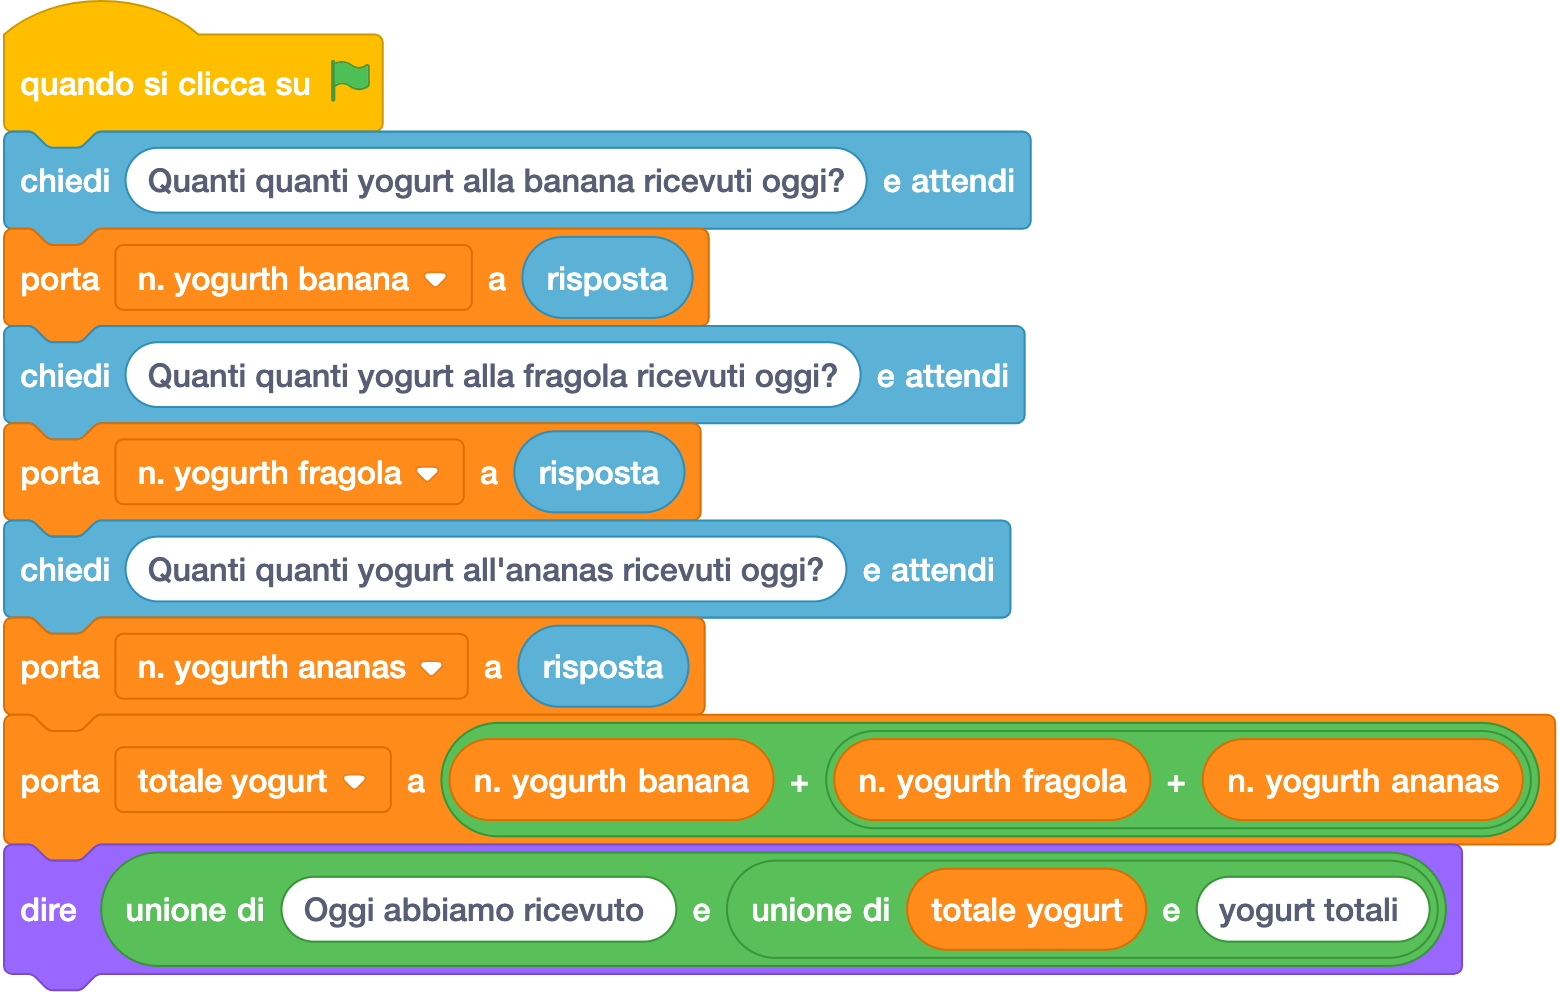
\includegraphics[width=0.8\linewidth]{img/cap2-scratch-programma.png}\label{credito:cap2-scratch-programma-1}
\end{center}

Ogni giorno, il responsabile potrà eseguire sul proprio computer questo programma senza più pensare a quale sia il procedimento: il computer eseguirà fedelmente le istruzioni al posto suo, gli chiederà in input i dati, e gli mostrerà il risultato.

Nella pratica scolastica può capitare di utilizzare il termine \textbf{algoritmi} per indicare solo le procedure che le alunne e gli alunni eseguono a volte meccanicamente (es. l'algoritmo per eseguire la divisione in colonna), cosa che può veicolare una visione procedurale della conoscenza lontana dalla comprensione concettuale e dal pensiero critico \parencite{crippa-etal-2025}. Questo è molto lontano dal senso informatico: infatti, gli informatici non hanno interesse a eseguire procedure sempre uguali e ripetitive--abbiamo inventato i computer proprio per eseguirle al posto nostro! Gli informatici sono molto più interessati a \textbf{inventare algoritmi} che risolvano problemi generali che si prestano poi ad essere automatizzati.


\subsection{Programmatore o esecutore?}


Se in generale gli informatici non amano essere ``esecutori'', per imparare l'informatica può essere utile, a volte, ``fare finta di essere un computer'', cioè eseguire alla lettera (secondo una precisa semantica) solo un insieme definito e limitato di istruzioni. Questo aiuta, quando si assumerà invece il ruolo di programmatori, a descrivere le elaborazioni che ci interessano in modo preciso e tenendo conto di ogni aspetto, senza lasciare nulla di implicito.

In alcune attività didattiche per l'introduzione dell'Informatica a scuola, però, viene posto l'accento solo sul ruolo di esecutore. È importante che le alunne e gli alunni riescano, a un certo punto, a costruire i propri programmi. Per questo motivo, nelle attività proposte in questa guida espliciteremo sempre quale ruolo (esecutore, programmatore o entrambi) assumono alunne e alunni, indicandoli con le seguenti icone.

\begin{center}
\ruoloProgrammatore\qquad\ruoloEsecutore
\end{center}

\begin{rimandiquaderno}
Anche nel volume studente vengono chiariti i ruoli di esecutore (ingranaggi) e programmatore (blocchetto verde), con due icone diverse.
\end{rimandiquaderno}

\section{Riferimenti}\label{riferimenti-1}

\printbibliography[heading=none,keyword={cap2},notcategory={attivita}]


% !TeX root = main.tex
\chapterimage{chapter-03-algoritmi-quotidiani.jpg}
\chapter{Algoritmi quotidiani}\label{algoritmi-quotidiani}

In questo capitolo proponiamo attività didattiche per una lettura algoritmica di molte delle attività che facciamo ogni giorno e che seguono una sequenza di passi. Infatti, per vestirci, cucinare o realizzare un modello con i mattoncini LEGO®, compiamo azioni che, se osservate dall'esterno, assomigliano molto a un algoritmo. Esploreremo come descrivere algoritmi relativi ad attività quotidiane in modo chiaro, preciso e non ambiguo, mettendo in luce come ciò che per chi descrive sembri ``ovvio'' possa essere interpretato in modi diversi da chi ascolta.

Dal punto di vista informatico, quando un algoritmo viene espresso in un linguaggio che il computer può ``capire'', viene chiamato \textbf{programma}. Il computer esegue il programma solo quando glielo ``chiediamo''. Il computer eseguirà solo ciò che è stato scritto, alla lettera e passo dopo passo, senza intuire o indovinare ciò che non è stato esplicitato e senza fare domande intermedie. Se durante o al termine dell'esecuzione qualcosa non ha funzionato, il programmatore, attraverso la pratica del debugging (vedi~\ref{debug}), potrà esaminare il comportamento dell'esecutore, individuare l'errore e modificare la sequenza.

Le attività di questa sezione propongono alcuni esempi di pratiche didattiche che incarnano le idee mostrate nei video del Capitolo~\ref{capitolo-1-introduzione} (sezione~\ref{pensiero-computazionale}), cioè la sfida del video \emph{Exact Instructions Challenge} per il panino con il burro di arachidi e il video del maestro Manzi sul lavarsi i denti. Potrete poi sbizzarrirvi nel progettare molte altre attività simili declinandole nel modo più opportuno alle vostre classi e scegliendo ambientazioni che diano significato e motivazione (ad esempio le regole di un gioco motorio, un laboratorio artistico, una storia inventata da alunni e alunne).

\section{Traguardi e obiettivi generali }\label{traguardi-e-obiettivi-generali}

\begin{itemize}
\item
  Scomporre un compito complesso in una sequenza di istruzioni elementari e ben definite.
\item
  Ordinare le istruzioni in modo coerente.
\item
  Utilizzare un linguaggio chiaro, preciso e non ambiguo per descrivere istruzioni.
\item
  Immedesimarsi nel punto di vista dell'esecutore, anticipando possibili fraintendimenti.
\item
  Riconoscere e correggere ambiguità nelle istruzioni.
\item
  Attuare pratiche di debugging.
\item
  Progettare e utilizzare un linguaggio condiviso per descrivere azioni.
\end{itemize}

\section{Prerequisiti }\label{prerequisiti}

Le attività proposte non richiedono particolari conoscenze informatiche pregresse: è sufficiente che alunni e alunne sappiano seguire e dare istruzioni in linguaggio naturale e ordinare nel tempo le fasi di una storia o di un'azione quotidiana. Per l'Attività 3 è utile che abbiano già incontrato le principali forme geometriche e abbiano avuto qualche esperienza di composizione con figure usando costruzioni di vario tipo.

Alcune attività sono progettate per essere proposte a chi non ha ancora raggiunto un livello di apprendimento della letto-scrittura adeguato ma, una volta che tali abilità strumentali saranno acquisite, sarà possibile proporre richieste più articolate e sfidanti.

\section{Contenuti, in breve }\label{contenuti-in-breve}

Questo capitolo contiene attività pensate per capire cosa significhi sviluppare una lettura algoritmica di un compito: scomporlo in istruzioni essenziali, metterle in ordine e formularle con precisione. Riprendendo quanto visto nel Capitolo~\ref{fondamentali-di-informatica} sulle istruzioni, vedremo come:

\begin{itemize}
\item
  definire le \textbf{istruzioni} elementari per raggiungere un certo obiettivo;
\item
  stabilire la \textbf{sequenza} corretta di istruzioni, cioè come ordinarle per ottenere un certo effetto;
\item
  \textbf{esprimere le istruzioni} in modo chiaro e non ambiguo.
\end{itemize}

\textbf{Attività 1 -- Sequenze e ordine}: alunni e alunne scompongono azioni o storie in istruzioni elementari, le mettono in sequenza e sperimentano cosa cambia (o non cambia) quando si altera l'ordine, per capire perché in un algoritmo l'ordine delle istruzioni è fondamentale, e talvolta sequenze diverse possono produrre lo stesso risultato.

\textbf{Attività 2 -- Istruzioni e programmi}: attraverso la richiesta di eseguire programmi dati e poi di inventarne di nuovi si introduce l'idea di \emph{Manuale delle istruzioni} che definisce ``quali istruzioni esistono e che cosa fanno''.

\textbf{Attività 3 -- Descrivere configurazioni geometriche}: far ricostruire una configurazione geometrica a un esecutore umano che segue le istruzioni alla lettera (senza interpretare né fare domande) e migliorare iterativamente le descrizioni tramite debugging, per arrivare a un linguaggio condiviso e rigoroso.

\section{Modalità di lavoro }\label{modalituxe0-di-lavoro}

Tutte le attività che seguono possono essere svolte in classe.

\begin{itemize}
\item
  Si alterneranno fasi di lavoro a coppie con momenti di confronto collettivo o a piccoli gruppi.
\item
  Lo spazio deve permettere di lavorare a coppie in modo che i membri di ciascuna coppia possano comunicare tra loro agevolmente.
\item
  Sarà importante osservare lo svolgimento delle varie attività tenendo traccia delle parole e delle produzioni di alunni e alunne (ad esempio, fornendo schede strutturate per scrivere o disegnare, ma anche scattando foto alle loro produzioni) da usare a supporto di discussioni collettive.
\end{itemize}

In tutte le proposte è cruciale mantenere netta la distinzione tra i ruoli di programmatore ed esecutore. Il \textbf{programmatore} \guideiconProgrammatore\ ha il compito di progettare e scrivere l'intera sequenza di istruzioni prima dell'esecuzione, cercando di prevedere come verranno interpretate. L'\textbf{esecutore} \guideiconEsecutore, invece, deve limitarsi a seguire le istruzioni alla lettera, senza ``aggiustare'' ciò che non è stato specificato e senza introdurre interpretazioni personali.

Questa distinzione rende visibile un'idea chiave: l'output di un programma non è ``l'intenzione'' di chi lo ha scritto, ma ciò che è effettivamente espresso nelle istruzioni disponibili e nel loro ordine.

Un ulteriore punto di attenzione riguarda il modo in cui le istruzioni vengono formulate: il linguaggio naturale è intrinsecamente ambiguo e dipende dal contesto, dalle conoscenze e dalle inferenze di chi ascolta o legge. Proprio per questo, molte attività mirano a far emergere ambiguità tipiche (``quanto?'', ``dove?'', ``rispetto a cosa?'', ``con quale orientamento?'') e a costruire progressivamente convenzioni condivise (ad esempio un \emph{manuale delle istruzioni}, introdotto in~\ref{manuale-delle-istruzioni}, o un lessico comune per descrivere posizioni e relazioni tra figure). Questo passaggio prepara il terreno per comprendere perché in informatica si introducono \textbf{linguaggi formali}: essi non eliminano la complessità del problema, ma rendono esplicite le regole di scrittura e di interpretazione, così che la stessa istruzione, nello stesso contesto formale, venga interpretata dall'esecutore in modo sempre uguale e prevedibile.

\section{Attività 1: sequenze e ordine}

Come abbiamo visto nel Capitolo~\ref{fondamentali-di-informatica}, le istruzioni date a un elaboratore vengono eseguite in sequenza e cambiarne l'ordine produce, in generale, risultati diversi. Quindi, sarà importante proporre attività in cui alunni e alunne possano riflettere sull'importanza di seguire o rispettare un ordine preciso quando, ad esempio, si scompongono attività quotidiane o storie in una sequenza di momenti.

\subsection{Preparazione}

\begin{itemize}
\item
  Stampare e ritagliare diverse immagini che raffigurano momenti di un'attività o scene di una storia.
\item
  Munirsi di post-it (per disegnare o scrivere istruzioni, numeri, parole chiave).
\end{itemize}

\subsection{Descrizione di proposte didattiche }\label{descrizione-di-proposte-didattiche}

\subsubsection{Riordinare delle immagini date}
\ruoliattivita{\ruoloProgrammatore}

In questo tipo di proposta a ciascuno viene consegnato un insieme di carte che raffigurano i diversi passi da fare per raggiungere un dato obiettivo (ad esempio avere i denti puliti, avere lo zaino pronto, andare a scuola) o di una storia. Le carte vengono inizialmente consegnate non ordinate e la richiesta è quella di metterle in ordine, anche eventualmente numerando i vari passi.

\subsubsection{Disegnare immagini o scrivere istruzioni in ordine}
\ruoliattivita{\ruoloProgrammatore}

In questo tipo di proposta a ciascuno viene chiesto di scegliere una storia che conosce o un'attività, suddividerla in momenti ordinati e poi descrivere ciascun momento con un'immagine o un breve testo (ad esempio su singoli foglietti o post-it da disporre in sequenza).

\subsubsection{Cambiare l'ordine e studiarne gli effetti}
\ruoliattivita{\ruoloProgrammatore\quad\ruoloEsecutore}


In questo tipo di proposta a ciascuno viene richiesto di esplorare cosa accade cambiando l'ordine delle istruzioni di una sequenza data. 

Sarà importante proporre anche situazioni in cui l'ordine di alcune
istruzioni può essere scambiato senza modificare il risultato finale.

Consideriamo, ad esempio, l'azione di preparare lo zaino. Una possibile sequenza consiste nell'\textbf{aprire lo zaino}, \textbf{prendere i libri}, \textbf{mettere i libri nello zaino} e infine \textbf{chiudere lo zaino}.

\begin{figure}[htbp]
    \centering
    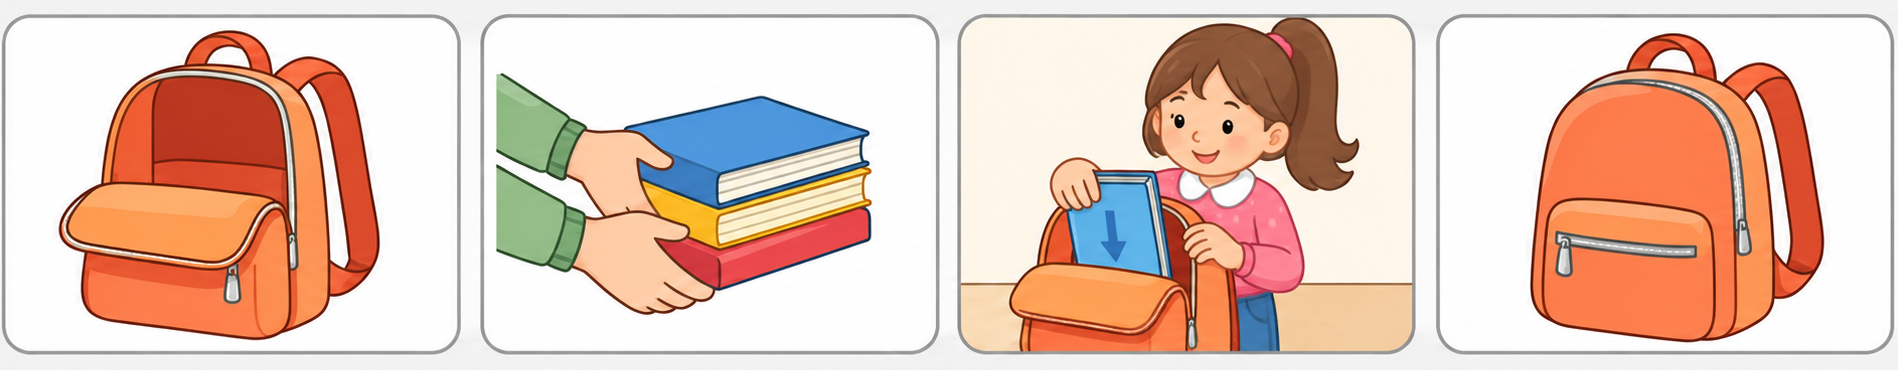
\includegraphics[width=0.95\linewidth]{img/cap3-sequenza1.png}
    % \caption{Una possibile sequenza di azioni per preparare lo zaino.}
    % \label{fig:cap3-sequenza1}
\end{figure}

Le prime due azioni, tuttavia, possono essere eseguite anche nell'ordine inverso: si possono prima \textbf{prendere i libri} e poi
\textbf{aprire lo zaino}, proseguendo quindi nello stesso modo.

\begin{figure}[htbp]
    \centering
    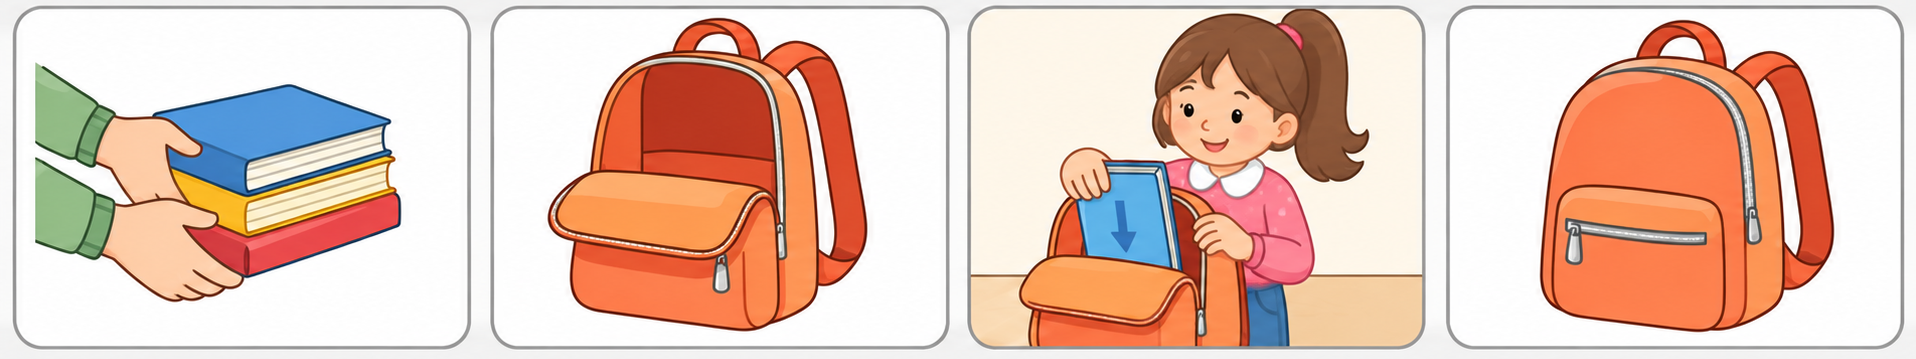
\includegraphics[width=0.95\linewidth]{img/cap3-sequenza2.png}
    % \caption{Una sequenza alternativa che produce lo stesso risultato.}
    % \label{fig:cap3-sequenza2}
\end{figure}

Il risultato non cambia, perché queste due azioni sono indipendenti
l'una dall'altra. Non tutte le azioni della sequenza possono però essere scambiate liberamente: per esempio, è necessario aprire lo zaino prima di inserirvi i libri e chiuderlo solo dopo averli inseriti.

Il confronto tra le due sequenze permette quindi di introdurre, in modo intuitivo, l'idea che alcune istruzioni possono essere scambiate senza effetti sul risultato, mentre tra altre esistono vincoli di precedenza.

\subsubsection{Inventare storie ``buffe''}
\ruoliattivita{\ruoloProgrammatore\quad\ruoloEsecutore}

Oltre a trovare la sequenza corretta, si può proporre una variante creativa: inventare ``storie buffe'' mescolando l'ordine delle scene. In questo caso, la sequenza prodotta diventa un dispositivo narrativo, un artefatto da raccontare, disegnare o persino mettere in scena. Gli errori o le sequenze ``sbagliate'' diventano risorsa: come suggerisce Rodari nella sua \emph{Grammatica della fantasia}, l'ordine alterato può generare narrazioni impreviste e divertenti, insegnando a ``smontare e rimontare'' le storie come fossero costruzioni.

\subsection{Contenuto informatico }\label{contenuto-informatico}

In informatica, la \textbf{sequenza di istruzioni} è la struttura di base (vedi~\ref{elementi-comuni}) su cui si costruisce ogni programma. Prima di introdurre concetti più complessi come le \textbf{selezioni} (\emph{se-allora}) o le \textbf{ripetizioni} (\emph{ripeti}), è essenziale che alunni e alunne comprendano a fondo cosa significhi eseguire azioni in un ordine preciso e senza ambiguità.

Le attività descritte permettono di lavorare su alcune idee chiave:
\begin{itemize}
\item
  Ogni azione deve essere descritta in modo esplicito, senza sottintesi;
\item
  L'ordine conta: modificare la sequenza può cambiare radicalmente il risultato;
\item
  Programmare richiede pianificazione: occorre pensare prima di agire e prevedere cosa farà l'esecutore;
\end{itemize}

Acquisire familiarità con la sequenza e con la capacità di pianificare è il primo passo della programmazione: solo dopo aver consolidato questi aspetti sarà possibile introdurre in modo efficace altre strutture fondamentali.

\section{Attività 2: istruzioni e programmi}

Un programma è una sequenza di istruzioni, scritte in un qualche linguaggio di programmazione. Prima di affrontare l'idea di ``linguaggio di programmazione'', e dopo aver lavorato su ordine e sequenza, sarà importante lavorare sulla formulazione di istruzioni da mettere in sequenza per scrivere ``programmi''\footnote{Come anticipato in \ref{manuale-delle-istruzioni}, per poter parlare di programmi veri e propri è necessario che l'esecutore sia meccanico e non umano. In questo capitolo, a partire dall'Attività 2, sarà possibile parlare intuitivamente di programmi solo a patto che chi assumerà il ruolo dell'esecutore si comporti ``come se fosse un computer'' ed esegua alla lettera le istruzioni per come descritte nel \emph{Manuale delle istruzioni}.}. In questo insieme di attività viene introdotto il \emph{Manuale delle istruzioni} (vedi~\ref{manuale-delle-istruzioni}) che, idealmente, contiene l'elenco di tutte e sole le istruzioni disponibili, ciascuna accompagnata dalla descrizione precisa e univoca del suo effetto.

\subsection{Preparazione }\label{preparazione}

\begin{itemize}
\item
  Istruzioni già stampate (per attività motorie o di altro tipo).
\item
  Post-it per scrivere istruzioni.
\end{itemize}

\subsection{Descrizione di possibili attività }\label{descrizione-di-possibili-attivituxe0}

\subsubsection{Eseguire programmi dati}

\ruoliattivita{\ruoloEsecutore}

In questo tipo di proposta vengono forniti dei programmi costituiti da sequenze di istruzioni che si riferiscono, ad esempio, ad attività motorie da eseguire (come brevi balletti o combinazioni di gesti). Ad alunni e alunne viene richiesto di eseguire il programma.


Dopo averlo eseguito, può essere utile proporre di compilare insieme il \emph{Manuale delle istruzioni} in cui esplicitare quali sono le istruzioni disponibili (o usate nel programma) e, per ciascuna, descrivere che effetto ha. Si potrebbe impostare il \emph{Manuale delle istruzioni} come una tabella del tipo:


\begin{center}
\manualeimpostazioni
\begin{tabular}{|J{\dimexpr0.50\linewidth-2\tabcolsep-3\arrayrulewidth/2\relax}|J{\dimexpr0.50\linewidth-2\tabcolsep-3\arrayrulewidth/2\relax}|}
\arrayrulecolor{guideManualeBordo}
\hline
\manualetitolo{2}{\ldots}
\manualeintestazione
\rule{0pt}{1.4em} & \\
\hline
\rule{0pt}{1.4em} & \\
\hline
\end{tabular}
\manualeripristinacolore
\end{center}



Ad esempio, considerando il programma seguente:

\begin{pseudocodice}
RIPETI 3 VOLTE:
    BATTI LE MANI
    BATTI I PIEDI
    FAI UN SALTO
    DIRE "COCCODÈ"
\end{pseudocodice}


il \emph{Manuale delle istruzioni} conterrà:

\begin{itemize}
\item
  nella colonna a sinistra, le singole istruzioni separate, cioè: ``ripeti 3 volte'', ``batti le mani'', ``batti i piedi'', ``fai un salto'', ``dire coccodè'';
\item
  nella colonna a destra, la spiegazione verbale di cosa significa ciascuna istruzione. Questo passaggio è tutt'altro che ovvio e sarà necessario esplicitare molti aspetti. Ad esempio, per l'istruzione ``batti le mani'': quante volte? E vanno battute tra loro o su un tavolo? E cosa significa ``batti i piedi''?
\end{itemize}

Non ci sono risposte corrette a priori: basta solo cercare di formulare la descrizione delle istruzioni nel modo più preciso e meno ambiguo possibile. Consigliamo di realizzare la tabella come attività collettiva in classe in modo da poter raccogliere tutte le proposte, condividerle con alunni e alunne e avviare una riflessione per arrivare a un \emph{Manuale delle istruzioni} condiviso.


\subsubsection{Dato il manuale delle istruzioni, inventare programmi}

\ruoliattivita{\ruoloProgrammatore}

In questo tipo di proposta viene fornito l'insieme delle istruzioni disponibili (sotto forma di \emph{Manuale delle istruzioni}) e si chiede ad alunni ed alunne di inventare dei programmi. Si può proporre il lavoro a coppie, in modo che a turno ciascuno possa comportarsi da esecutore del programma del compagno o della compagna.

Al termine dell'attività sarà importante raccogliere e commentare tutti i diversi programmi per rendere esplicito che, dato un piccolo insieme di istruzioni, con queste si possono scrivere moltissimi programmi diversi.

\subsubsection{Inventare istruzioni e programmi}
\ruoliattivita{\ruoloProgrammatore}


In questo tipo di proposta si chiede ad alunni ed alunne di inventare un set di istruzioni per poter realizzare un'attività (ad esempio un balletto), scriverne il \emph{Manuale delle istruzioni} e poi inventare almeno 2-3 programmi diversi come sequenza delle proprie istruzioni. Anche in questo caso è utile il lavoro a coppie, in modo che ciascuno a turno possa comportarsi da esecutore del programma del compagno o della compagna.

\subsubsection{Schede strutturate}


Con alunni ed alunne più grandi, può essere utile usare delle schede strutturate (es. vedi schede~\ref{scheda-inventare-1} e~\ref{scheda-inventare-2} nelle pagine seguenti) in cui:\label{richiamo:cap03-schede-1ab}
% Inserite come float nella pagina successiva al richiamo.
\begin{scheda}[A1][3]
\phantomsection\label{scheda-inventare-1}
\schedatitolo{INVENTARE ISTRUZIONI E PROGRAMMI}
\schedaparte{\scalebox{1.35}{\guideiconProgrammatore}}{1) Parte per il programmatore}
\hspace*{12mm}\begin{minipage}{\dimexpr\linewidth-12mm\relax}
Inventa delle istruzioni con cui creare tanti nuovi programmi!\par
Completa il \emph{Manuale delle istruzioni}:
\end{minipage}\par
\vspace{8mm}
\begingroup
\setlength{\tabcolsep}{3mm}
\setlength{\arrayrulewidth}{0.6pt}
\arrayrulecolor{black!55}
\renewcommand{\arraystretch}{1}
\noindent\begin{tabular}{|p{\dimexpr.5\linewidth-2\tabcolsep-1.5\arrayrulewidth\relax}|p{\dimexpr.5\linewidth-2\tabcolsep-1.5\arrayrulewidth\relax}|}
\hline
\rowcolor{black!10}
\multicolumn{1}{|c|}{\rule[-3mm]{0pt}{10mm}\fontsize{15}{18}\selectfont\textbf{ISTRUZIONI DISPONIBILI}} &
\multicolumn{1}{c|}{\fontsize{15}{18}\selectfont\textbf{EFFETTO}} \\
\hline
\rule{0pt}{24mm} & \\\hline
\rule{0pt}{24mm} & \\\hline
\rule{0pt}{24mm} & \\\hline
\rule{0pt}{24mm} & \\\hline
\rule{0pt}{24mm} & \\\hline
\end{tabular}\par
\endgroup
\end{scheda}

\begin{scheda}[A2][3]
\phantomsection\label{scheda-inventare-2}
E ora scrivi qualche programma da far eseguire a un compagno o una compagna:\par
\vspace{7mm}
\begingroup
\setlength{\fboxsep}{0pt}
\setlength{\fboxrule}{0.6pt}
\noindent\fcolorbox{black!55}{white}{\rule{0pt}{88mm}\hspace{\dimexpr\linewidth-2\fboxrule\relax}}\par
\endgroup
\vspace{7mm}
Lo ha eseguito in maniera corretta? \schedacasella\ Sì\quad\schedacasella\ No\par
\vspace{6mm}
\schedaparte{\scalebox{1.35}{\guideiconEsecutore}}{2) Parte per l'esecutore}
\hspace*{12mm}\begin{minipage}{\dimexpr\linewidth-12mm\relax}
Quali istruzioni non erano chiare?\par
\vspace{5mm}
{\color{black!55}%
\hrule height 0.6pt\vspace{8mm}
\hrule height 0.6pt\vspace{8mm}
\hrule height 0.6pt\vspace{8mm}
\noindent\rule{.31\linewidth}{0.6pt}\par}
\vspace{4mm}
\textbf{3) Parte da fare insieme}\par
Modificate il \emph{Manuale delle istruzioni} in modo da rendere la descrizione dell'effetto di ciascuna istruzione più chiara.
\end{minipage}\par
\end{scheda}

\begin{itemize}
\item
  i programmatori scrivono il proprio \emph{Manuale delle istruzioni} e i propri programmi;
\item
  gli esecutori danno un feedback sulla chiarezza delle istruzioni;
\item
  alla fine, insieme, apportano modifiche al \emph{Manuale delle istruzioni} per riflettere su come descrivere le istruzioni disponibili in maniera chiara, precisa e priva di ambiguità.
\end{itemize}

Al termine dell'attività sarà importante raccogliere e commentare i vari \emph{Manuali delle istruzioni} per riflettere collettivamente su come descrivere le istruzioni disponibili.

\subsubsection{Attività preparatoria}

\ruoliattivita{\ruoloProgrammatore\quad\ruoloEsecutore}

Come attività preparatoria a proposte di questo tipo, si può chiedere di scrivere per qualcun altro le istruzioni per fare un panino al cioccolato, che poi dovrà eseguirle alla lettera e si valuterà insieme se sono precise. Si può anche mostrare e commentare in classe il video del maestro Manzi\footnote{\linkbreve{manzi} (DAL MINUTO 8:44)}.


\subsection{Contenuto informatico }\label{contenuto-informatico-1}

In questa attività il \emph{Manuale delle istruzioni} gioca metaforicamente il ruolo della \textbf{sintassi} (le regole del linguaggio) e della \textbf{semantica} (il significato delle istruzioni) nei linguaggi di programmazione: definisce quali istruzioni esistono e che cosa fanno. I programmi sono le sequenze di istruzioni scritte usando esclusivamente le istruzioni presenti nel \emph{Manuale delle istruzioni}, mentre l'esecutore rappresenta il computer, che esegue il programma alla lettera senza poter fare domande né ``indovinare'' ciò che non è stato scritto.

Le attività proposte permettono di lavorare su alcune idee chiave dell'informatica:

\begin{itemize}
\item
  un insieme limitato di istruzioni può generare moltissimi programmi diversi;
\item
  ogni istruzione deve avere un effetto descritto in modo esplicito e non ambiguo, perché l'esecutore esegue solo le istruzioni che riceve (se in una sequenza che descrive come fare un panino al cioccolato manca, ad esempio, ``apri il barattolo'', l'esecutore può limitarsi ad appoggiare il barattolo chiuso sul pane);
\item
  per programmare serve pianificare: chi scrive il programma deve prevedere in anticipo come verrà interpretata ogni istruzione da chi esegue;
\item
  il debugging è un processo ciclico di prova, osservazione e revisione: gli errori non sono un fallimento, ma un'occasione per migliorare.
\end{itemize}

\section{Attività 3: descrivere configurazioni geometriche}

La Fase 1 di questa attività può essere svolta anche con alunni e alunne più giovani (classi prima e seconda primaria). La Fase 2 richiede invece di scrivere un testo e quindi è più adatta a partire dalla classe terza primaria.

\subsection{Preparazione }\label{preparazione-1}

\begin{itemize}
\item
  Stampare e ritagliare un tangram di carta per ciascuno\footnote{Un foglio con sei tangram colorati è disponibile in
\hrefbreve{tangram}{formato PNG} (\linkbreve{tangram}),
da stampare su A4 selezionando l'opzione ``Adatta alla pagina'' e ritagliare.
Fonte: \hreforiginale{https://commons.wikimedia.org/wiki/File:Tangrams_A4_Nevit.svg}{Nevit Dilmen, Wikimedia Commons} (\urloriginale{https://commons.wikimedia.org/wiki/File:Tangrams_A4_Nevit.svg});
licenza \hreforiginale{https://creativecommons.org/licenses/by-sa/3.0/deed.it}{CC BY-SA 3.0} (\urloriginale{https://creativecommons.org/licenses/by-sa/3.0/deed.it}).}.
\item
  Procurarsi anche altri tipi di forme geometriche di carta o altro materiale (es. legno o plastica).
\end{itemize}

\subsection{Fase 1 - descrizione verbale }\label{fase-1---descrizione-verbale}

\ruoliattivita{\ruoloProgrammatore\quad\ruoloEsecutore}

\subsubsection{Obiettivo}

Accordarsi su un linguaggio condiviso per disambiguare istruzioni date.

\subsubsection{Descrizione}\label{descrizione}

Alunni e alunne vengono divisi in coppie\footnote{Se il numero totale è dispari, si può formare un gruppo di 3.} e a ciascun componente viene consegnato un tangram di carta. Le coppie si dispongono in modo da potersi ascoltare tra loro senza però vedere quello che ciascuno ha davanti a sé. Quindi, ad esempio, potranno sedersi di spalle oppure di fronte, ma mettendo un divisorio in mezzo.

Si stabiliscono due ruoli, quello di \textbf{programmatore} \guideiconProgrammatore\ e quello di \textbf{esecutore} \guideiconEsecutore.

La Fase 1 consiste di \textbf{3 diversi turni di gioco, ciascuno ripetuto due volte} per permettere ad alunni e alunne di scambiarsi i ruoli\footnote{Se c'è un gruppo da 3, si organizzano i turni di gioco in modo che ci sia un programmatore e due esecutori indipendenti tra loro.}. In ogni turno di gioco, la dinamica è sempre la stessa:

\begin{itemize}
\item
  chi ha il ruolo di programmatore dovrà creare una composizione di figure geometriche usando tutti e sette i pezzi del tangram;
\item
  una volta creata la composizione, dovrà descriverla all'esecutore per fargliela ricreare esattamente identica. Non è permesso indicare, mimare o alzarsi per guardare il lavoro del compagno o della compagna: l'unico canale di comunicazione che si può usare è la parola;
\item
  quando l'esecutore ritiene di aver terminato la sua ricostruzione, deve dichiararlo e la configurazione originale e quella ricostruita possono essere confrontate per valutare se sono esattamente identiche e sovrapponibili pezzo per pezzo oppure no.
\end{itemize}

Ciò che cambia tra un turno e l'altro è la possibilità di interazione da parte di chi ha il ruolo di esecutore:

\begin{itemize}
\item
  Nel \textbf{primo turno di gioco}, l'esecutore può fare al programmatore \textbf{qualsiasi domanda} di chiarimento che riterrà opportuna.
\item
  Nel \textbf{secondo turno di gioco}, l'esecutore ha a disposizione \textbf{solo tre domande di chiarimento} da fare al programmatore.
\item
  Nel \textbf{terzo turno di gioco}, l'esecutore \textbf{non potrà fare alcuna domanda} al programmatore.
\end{itemize}

Durante i vari turni di gioco, l'insegnante potrà girare tra le varie coppie e, dopo aver osservato gli scambi comunicativi senza intervenire, potrà facilitare l'emergere delle prime riflessioni ponendo delle domande stimolo alla fine di ciascun turno.

\begin{domandestimolo}\label{domande-stimolo}

\begin{itemize}
\item
  Siete riusciti sempre a capirvi?
\item
  Quando non riuscivate a capirvi, da cosa dipendeva secondo voi?
\item
  (Rivolta al programmatore) Quali configurazioni hai trovato più difficili da descrivere?
\item
  (Rivolta all'esecutore) Quali istruzioni hai trovato più difficili da capire? E che domande facevi per capirle meglio?
\item
  Al prossimo turno di gioco a cosa farete maggiore attenzione per capirvi meglio?
\end{itemize}
\end{domandestimolo}

Al termine della Fase 1, si può proporre una discussione collettiva per condividere le osservazioni rispetto all'esperienza vissuta e raccogliere le caratteristiche di eventuali pattern di ambiguità emersi nei vari turni di gioco.

\subsection{Contenuto informatico }\label{contenuto-informatico-2}

Questa prima fase permette di distinguere diversi livelli di precisione con cui possono essere fornite istruzioni e prepara il terreno per la fase successiva. Inoltre, la progressiva riduzione delle domande di chiarimento (fino a nessuna domanda nel terzo turno di gioco) sottolinea la differenza fra una comunicazione dialogica tra umani e l'esecuzione di un programma da parte di un computer, che non può chiedere spiegazioni durante l'esecuzione.


\subsection{Fase 2 - descrizione scritta }\label{fase-2---descrizione-scritta}

\subsubsection{Obiettivo}\label{obiettivo}

Disambiguare la descrizione di una configurazione geometrica attraverso una pratica ispirata al debugging.

\subsubsection{Descrizione}

Alunni e alunne vengono divisi in un numero pari di gruppi da 3-4 persone ciascuno. Si mettono a disposizione della classe nuovi set di forme geometriche varie che siano diversi dal tangram\footnote{Potranno essere nuove sagome di carta o cartone o altri tipi di costruzioni in plastica o legno. Per avere pezzi a sufficienza per tutti i gruppi, sarà necessario averne un buon numero.}. Ciascun gruppo sceglie un set di almeno 5 nuove forme con cui realizzare la propria configurazione geometrica.

I vari gruppi si dispongono nello spazio dell'aula così da riuscire a lavorare in modo abbastanza riservato rispetto agli altri (ad esempio creando un'\,``isola di lavoro'' per ciascun gruppo).

La Fase 2 si divide in tre parti. La prima parte è preparatoria ed è dedicata alla realizzazione della configurazione geometrica da descrivere. La seconda parte è dedicata alla scrittura del testo che descrive la propria configurazione. La terza è dedicata al debugging del testo che avviene osservando un altro gruppo mentre lo interpreta e ricostruisce la figura seguendo le istruzioni.

\begin{itemize}
\item
  \textbf{Parte 1. Preparazione della configurazione geometrica.}
  Come prima cosa, ogni gruppo crea con i pezzi scelti la propria configurazione geometrica e la disegna in un foglio pezzo per pezzo: questo disegno andrà piegato e nascosto perché rappresenterà la soluzione.
\item
  \textbf{Parte 2. Scrittura del testo.}
  \ruoliattivita{\ruoloProgrammatore}
  Ogni gruppo dovrà scrivere un testo, il più preciso e meno ambiguo possibile, che contenga le istruzioni affinché un altro gruppo possa, seguendole alla lettera, ricostruire esattamente la stessa configurazione. Ci sono due aspetti importanti da considerare:

  \begin{itemize}
  \item
    il testo \textbf{non può contenere disegni ma solo istruzioni verbali};
  \item
    le informazioni scritte nel testo sono tutto ciò che il gruppo che deve ricostruire la configurazione avrà a disposizione: \textbf{chi ricostruisce non potrà fare domande}.
  \end{itemize}

  Una volta terminata la scrittura del testo, sarà importante smontare la configurazione geometrica costruita per non farla vedere a nessuno.
\item
  \textbf{Parte 3. Debugging.}
  \ruoliattivita{\ruoloEsecutore\quad\ruoloProgrammatore}
  Quando due gruppi (che per comodità chiamiamo A e B) hanno terminato la scrittura del proprio testo:

  \begin{enumerate}
  \def\labelenumi{\arabic{enumi}.}
  \item
    il gruppo A si sposta nella postazione del gruppo B e consegna il proprio testo e i pezzi scelti;
  \item
    il gruppo B dovrà seguire alla lettera le istruzioni scritte dal gruppo A e ricostruire la configurazione. Nel leggere e interpretare il testo, i componenti del gruppo B dovranno \textbf{eseguire esattamente ciò che c'è scritto andando ``a caccia'' di ambiguità}, cioè chiedendosi in ogni passaggio: \emph{quante configurazioni diverse si possono descrivere con queste istruzioni?}
  \item
    nel frattempo, il gruppo A osserva in silenzio e senza intervenire il gruppo B mentre legge, interpreta il testo ed esegue la costruzione;
  \item
    quando il gruppo B termina la ricostruzione, il gruppo A può riprendere il proprio testo e modificarlo alla luce di quello che ha osservato durante l'interpretazione del gruppo B;
  \item
    il gruppo A può riconsegnare il testo modificato al gruppo B che farà un nuovo giro di lettura e ricostruzione;
  \item
    al termine della seconda ricostruzione del punto 5, il gruppo A mostrerà il disegno-soluzione da confrontare con la figura ricostruita dal gruppo B.
  \end{enumerate}
\end{itemize}

La figura~\ref{fig:debug-gruppi} schematizza i passaggi da 1 a 6; poi, si ricomincia ripetendo i passaggi da 1 a 6 ma scambiando i due gruppi (quindi il gruppo A sarà l'interprete del testo scritto dal gruppo B, che osserverà in silenzio per poi modificare il proprio testo sulla base di quanto osservato).



In questa Fase 2 dell'attività il testo scritto dal gruppo gioca il ruolo del programma, mentre il gruppo che lo legge e costruisce la figura gioca il ruolo dell'esecutore.

\begin{attenzione}[Aspetti a cui fare attenzione]\label{aspetti-a-cui-fare-attenzione}


Perché tutto funzioni al meglio, è importante chiarire che:


\begin{itemize}
\item
  l'obiettivo comune dei due gruppi non è quello di ricostruire la figura ``giusta'' ma scrivere testi e istruzioni il più precisi e meno ambigui possibili. In particolare, quando si scrive il testo, l'obiettivo è evitare il più possibile ambiguità; quando si interpreta un testo, l'obiettivo è trovare più ambiguità possibili;
\item
  si fa debugging del testo e non delle persone (quindi, le osservazioni su passaggi poco chiari dovranno sempre essere espresse in termini di istruzioni che si possono scrivere più chiaramente o precisamente e mai in termini di ``compagni che non sanno spiegare'').
\end{itemize}
\end{attenzione}

Al termine della Fase 2 sarà possibile condurre una riflessione collettiva per condividere le osservazioni rispetto all'esperienza vissuta e raccogliere le strategie usate per chiarire e precisare meglio le descrizioni scritte.

\begin{domandestimolo}\label{domande-stimolo-1}

\begin{itemize}
\item
  Che differenze avete trovato tra la prima fase dell'attività e la seconda?
\item
  Quando osservavate gli altri interpretare il vostro testo, è successo qualcosa che non vi aspettavate? Se sì, cosa?
\item
  Quando osservavate gli altri interpretare il vostro testo, cosa vi è stato utile considerare per migliorarlo?
\item
  Quali regole di scrittura avreste potuto usare per scrivere dei testi chiari e precisi?
\end{itemize}
\end{domandestimolo}

\subsection{Contenuto informatico}\label{contenuto-informatico-3}

Il linguaggio naturale è ambiguo per natura e la sua interpretazione da parte delle persone dipende da chi sono quelle persone (dalle loro esperienze, da ciò che conoscono, eccetera). Tuttavia, l'attività appena descritta permette ad alunni e alunne di riflettere sull'importanza di stabilire un linguaggio convenzionale condiviso per esprimere le istruzioni in modo tale che chi le fornisce e chi le esegue le interpretino allo stesso modo. Porre attenzione su questo aspetto prepara il terreno per cogliere le caratteristiche dei linguaggi formali (linguaggi di programmazione) che sono ciò che permette e assicura che l'esecutore esegua una certa istruzione sempre allo stesso modo, senza ambiguità.

\begin{figure}
\centering
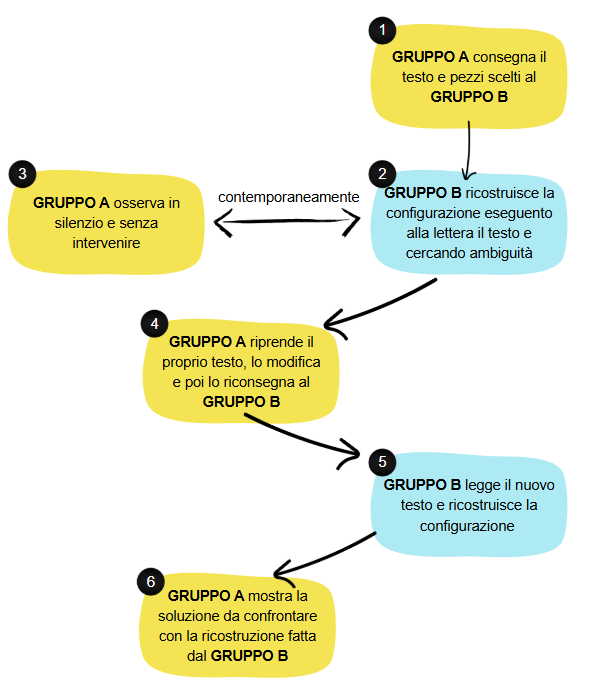
\includegraphics[width=\linewidth]{img/cap3-debug-gruppi.png}\label{credito:debug-luci-originali-1}
\caption{Schema dei passaggi di debugging (Attività 3, Fase 2, Parte 3) tra i due gruppi.}
\label{fig:debug-gruppi}
\end{figure}

\section{Possibili estensioni, variazioni e personalizzazioni }\label{possibili-estensioni-variazioni-e-personalizzazioni}


\subsection{Spunti per adattare le attività}

In caso di difficoltà:


\begin{itemize}
\item
  Diminuire il numero di elementi da gestire (es. il numero di immagini da riordinare o il numero di pezzi a disposizione per creare la configurazione geometrica).
\item
  Invece di chiedere di scrivere dei testi, fornire opzioni di testi già scritti tra cui scegliere quello corretto.
\end{itemize}

Come rendere le attività più sfidanti:

\begin{itemize}
\item
  Aumentare il numero o il tipo di elementi da gestire (ad esempio, nella Fase 2 dell'attività \emph{Descrivere configurazioni geometriche} si può proporre di lavorare su configurazioni tridimensionali).
\item
  Proporre una storia ``sbagliata'' in cui prima individuare le parti principali per poi riordinarle.
\end{itemize}

\section{Aspetti informatici }\label{aspetti-informatici}

In informatica, la sequenza di istruzioni è la struttura di base su cui si costruisce ogni programma. Prima di introdurre strutture più complesse come le selezioni (\emph{se-allora}) o le ripetizioni (\emph{ripeti}), è essenziale che gli alunni e le alunne comprendano a fondo cosa significhi eseguire azioni in un ordine preciso e senza ambiguità.

Queste attività sono particolarmente efficaci perché:

\begin{itemize}
\item
  evidenziano la differenza fra chi crea un programma (programmatore) e chi lo esegue (esecutore);



\item mostrano che un algoritmo deve essere pensato per un esecutore che può eseguire solo un certo insieme di istruzioni ben definito;

\item
  introducono il concetto di debugging come revisione e correzione della sequenza;
\item
  allenano la pianificazione, cioè la capacità di prevedere in anticipo tutti i passi necessari, organizzarli in modo logico e verificarne la completezza.
\end{itemize}

A differenza di una conversazione, in cui è possibile correggere passo-passo ciò che fa l'esecutore, solitamente quando si programma la sequenza viene scritta interamente prima dell'esecuzione\footnote{
  Tralasciamo per il momento forme più interattive di programmazione, che si stanno diffondendo oggi.
  }. Questo richiede un pensiero anticipatorio: occorre immaginare lo svolgimento dell'intero compito, prevedere le criticità e predisporre le istruzioni necessarie a evitarle.

Queste esperienze permettono ad alunni e alunne di esplorare alcune idee chiave:

\begin{itemize}
\item
  \textbf{Ogni azione deve essere descritta in modo esplicito}.
\item
  \textbf{L'ordine conta}: modificare la sequenza può cambiare radicalmente il risultato.
\item
  \textbf{Programmare richiede pianificazione}: occorre pensare prima di agire e prevedere cosa farà l'esecutore.
\item
  \textbf{Le regole condivise} sono indispensabili perché il messaggio sia interpretato nello stesso modo da chi lo scrive e da chi lo legge.
\item
  \textbf{Il debugging è parte del processo}: provare, osservare cosa non funziona, correggere e ripetere.
\end{itemize}

Acquisire familiarità con la sequenza, con la necessità di precisione e con la capacità di pianificare è il primo passo nel percorso di programmazione: solo dopo aver consolidato queste competenze sarà possibile introdurre in modo efficace altre strutture fondamentali come le istruzioni condizionali o le ripetizioni.

\section{Relazione con l'informatica nelle Indicazioni Nazionali 2025 }\label{relazione-con-linformatica-nelle-indicazioni-nazionali}

Relativamente alle Indicazioni Nazionali 2025, queste attività contribuiscono allo sviluppo delle seguenti competenze, obiettivi e conoscenze (queste ultime inserite nelle Indicazioni Nazionali 2025 a titolo di esempio, non prescrittive).


\subsubsection{Competenze (alla fine della scuola primaria) nella disciplina Matematica}


\begin{itemize}
\item
  \emph{Descrivere procedure per lo svolgimento di compiti pratici mediante algoritmi.}
\end{itemize}


\subsubsection{Obiettivi (alla fine della terza primaria) nella disciplina Matematica}


\begin{itemize}
\item
  \emph{Descrivere a parole attività della vita quotidiana tramite sequenze di passi precisi e non ambigui e saperle eseguire.}
\item
  \emph{Scrivere semplici programmi e verificare, mediante la loro esecuzione, se svolgono il compito previsto ed eventualmente correggerli}. Sebbene queste attività siano unplugged (senza computer), si va nella direzione di linguaggi formali con una sintassi e una semantica ben definite e non ambigue. Per questo sono una buona preparazione per questo obiettivo, poiché sono orientate alla progettazione e scrittura di programmi, e alla loro valutazione (controllo di correttezza, debugging, \ldots).

\end{itemize}


\subsubsection{Conoscenze (scuola primaria) nella disciplina Matematica}



\begin{itemize}
\item
  \emph{concetto di algoritmo e sua esecuzione rigorosa};
\item
  \emph{strutture di controllo fondamentali di un linguaggio di programmazione} (In questo capitolo si lavora in particolare sulla sequenza);
\item
  \emph{controllo di correttezza dei programmi}.
\end{itemize}

\section{Valore costruzionista }\label{valore-costruzionista}

Seguendo la prospettiva di Papert, l'apprendimento passa per la costruzione di artefatti significativi di vario tipo che possono essere mostrati, discussi e migliorati insieme. In questo processo, l'errore non è qualcosa da evitare ma è una risorsa, un'informazione preziosa che rende visibili ambiguità e sottintesi e spinge a rendere le istruzioni sempre più chiare. Sequenze ambigue, indicazioni incomplete o termini poco chiari diventano occasioni per riflettere, riformulare e affinare il proprio lavoro attraverso cicli di prova, osservazione e revisione (debugging). La progressione delle attività proposte in questo capitolo - dall'ordinamento di istruzioni fino allo stabilire un linguaggio convenzionale condiviso per \emph{descrivere configurazioni geometriche} - mette in evidenza un approccio tipico in informatica: affrontare la complessità scomponendo i problemi e stabilendo regole condivise che rendano le procedure eseguibili in modo prevedibile. In questo modo alunni e alunne imparano a progettare, verificare e migliorare le proprie soluzioni.

\section{Suggerimenti per ulteriori attività}\label{suggerimenti-per-ulteriori-attivituxe0-e-riferimenti}

Ulteriori attività e riferimenti possono essere reperiti ai seguenti collegamenti.

\printbibliography[heading=none,keyword={cap3},category={attivita}]

\begin{rimandiquaderno}
Se possiedi il volume studente \emph{Sulle orme di Milù -- Informatica}
(Mondadori Education, 2026), puoi usare i rimandi seguenti per affiancarlo
alle attività di questo capitolo.\par\smallskip

\begin{itemize}[leftmargin=*,itemsep=5pt,topsep=4pt]
\item \textbf{Attività 1 -- Sequenze e ordinamenti.} Le attività qui proposte sono analoghe a quelle delle pagine 2 e 3 intitolate RIORDINARE. Nell'attività a pagina 2, sono possibili due ordini (la prima istruzione può essere quella di aprire lo zaino o di prendere i libri).
\item \textbf{Attività 2 -- Istruzioni e programmi.} Le schede ISTRUZIONI E PROGRAMMI (pagg.~4--5) propongono le attività sulla formulazione e sull'esecuzione letterale delle istruzioni: a pag.~4 si trova il panino al cioccolato. Il programma esemplificato nell'Attività 2 della guida è quello della prima attività di pag.~5, rappresentato con blocchi colorati che richiamano i linguaggi visuali, come Scratch.
\item \textbf{Attività 3 -- Descrivere configurazioni geometriche.} Le schede DESCRIVERE UNA FIGURA (pagg.~6--7) si possono usare per preparare o rafforzare le due fasi dell'attività: pag.~6 per la Fase 1 e pag.~7 per la Fase 2. \textbf{Soluzione di pag.~6:} fra Alice e Bob, è Alice a fornire una descrizione che permette di individuare in modo univoco la figura corretta fra le due proposte.
\end{itemize}
\end{rimandiquaderno}


% !TeX root = main.tex
\chapterimage{chapter-04-movimenti-griglia.jpg}
\chapter{Movimenti su una griglia}\label{capitolo-4-movimenti-su-una-griglia}

Nel capitolo precedente abbiamo lavorato su situazioni quotidiane e giochi, in cui gli alunni e le alunne hanno sperimentato l'idea di descrivere \textbf{sequenze} di azioni e di osservare ciò che succedeva eseguendole.

In questo capitolo facciamo un passo avanti: ci spostiamo in un ambiente più strutturato, la griglia, che diventa il nostro campo di gioco.

Da un punto di vista informatico, la griglia è un contesto chiaro in cui formulare sequenze di \textbf{istruzioni} precise, osservare come un \textbf{esecutore} le interpreta, individuare eventuali errori e correggerli. È il modo più immediato per far capire ai bambini e bambine che un computer (o un robot) esegue sempre e solo ciò che ``gli diciamo'', senza intuire ciò che non è stato specificato.

Da un punto di vista delle altre discipline, come la matematica (ma non solo), muoversi su una griglia significa ragionare in termini di spazio, angoli, distanze, direzioni, coordinate. È un terreno ideale per materializzare concetti di geometria e di ragionamento spaziale in attività pratiche.

\section{Traguardi e obiettivi generali }\label{traguardi-e-obiettivi-generali-1}

\begin{itemize}
\item
  Pianificare sequenze di istruzioni ordinate per raggiungere un obiettivo definito.
\item
  Prevedere l'esecuzione di un programma, immaginando passo per passo cosa farà l'esecutore.
\item
  Verificare sperimentalmente l'esecuzione di un programma, confrontando le previsioni con il risultato.
\item
  Individuare e correggere errori (debugging) osservando gli effetti dell'esecuzione.
\item
  Comprendere il valore di un linguaggio preciso e condiviso, che consente di comunicare efficacemente sia con un computer sia tra esseri umani.
\item
  Riconoscere e utilizzare diversi sistemi di riferimento spaziali (ad es. destra/sinistra, punti cardinali) per descrivere movimenti e posizioni.
\end{itemize}

\section{Prerequisiti }\label{prerequisiti-1}

Gli alunni e le alunne avranno già svolto le attività del Capitolo~\ref{algoritmi-quotidiani} - Algoritmi quotidiani, quindi:

\begin{itemize}
\item
  dovrebbero già avere un'idea iniziale di \textbf{algoritmo}, inteso in modo informale come una sequenza di passi per raggiungere un obiettivo;
\item
  dovrebbero avere familiarità con il fatto che le istruzioni vengono eseguite da un esecutore (computer o umano ``che fa il computer''), nell'ordine in cui sono state scritte.
\end{itemize}

\section{Contenuti, in breve }\label{contenuti-in-breve-1}

Questo capitolo contiene attività a difficoltà crescente in cui i bambini e le bambine devono far completare delle ``missioni'' a un personaggio che si muove su un campo di gioco composto da una griglia (ad esempio, una griglia 8x8 disegnata sul pavimento, composta da 64 caselle). Può essere utile inserire l'attività in un contesto che dia senso alla missione e al personaggio. Ad esempio:

\begin{itemize}
\item
  il personaggio è Miguel e la sua missione è prendere un certo peluche usando la macchina con l'artiglio (Claw Crane);



\item il personaggio è un'ape che vola tra i fiori e la sua missione è impollinare più fiori possibili;



\item
  personaggio e missione sono ispirati a una storia letta in classe e poi simulata sulla griglia. Ad esempio, il personaggio è Cappuccetto Rosso e la sua missione è andare dalla nonna e portarle il pranzo, evitando il lupo per strada.
\end{itemize}

In particolare, vengono proposte 3 attività.

\textbf{Attività 1 -- Be my robot:} gli alunni e le alunne guidano un compagno-robot sulla griglia con istruzioni semplici in linguaggio naturale, sperimentando diversi modi per descrivere movimenti e posizioni.

\textbf{Attività 2 -- Be my more intelligent robot:} si arricchisce il linguaggio con istruzioni di ripetizione e selezione (``se\ldots{} allora\ldots''), per scrivere programmi più compatti e generali.

\textbf{Attività 3 -- Bee my robot:} gli stessi concetti vengono ripresi usando veri robot educativi che si muovono sulla griglia, programmati in anticipo tramite tasti o carte-istruzioni.

\section{Movimenti su una griglia e sistemi di riferimento }\label{movimenti-su-una-griglia-e-sistemi-di-riferimento}

Nelle attività discusse in questo capitolo, i bambini e le bambine imparano a scrivere istruzioni per far muovere un compagno/a su una griglia. L'attività si svolge in coppia o in piccolo gruppo: a turno, alcuni progettano e scrivono (o, in alcuni casi, dettano) le istruzioni per il movimento (cioè, interpretano il ruolo dei \textbf{programmatori} \guideiconProgrammatore) mentre altri le devono eseguire (cioè, interpretano il ruolo dell'\textbf{esecutore} \guideiconEsecutore).

Chi esegue il movimento lo fa in modo meccanico, senza aggiungere né indovinare nulla.

\begin{attenzione}\label{aspetto-a-cui-fare-attenzione}


Distinguere tra chi \textbf{pianifica} \guideiconProgrammatore\ e chi \textbf{esegue} \guideiconEsecutore\ è importante per avvicinare gli alunni e le alunne a un modo di pensare tipico dell'informatica. Il programmatore deve immaginare in anticipo cosa accadrà, scrivere le istruzioni correttamente e prevedere gli effetti di ciascuna istruzione. L'esecutore, invece, si comporta come un piccolo robot \emph{senza volontà}: segue ciò che è scritto, anche quando qualcosa non ha senso, aiutando così il gruppo a capire se il programma è stato progettato bene o va corretto.
\end{attenzione}


Le istruzioni riguardano i movimenti sulla griglia e si possono descrivere usando diversi sistemi di riferimento:

\begin{itemize}
\item
  \textbf{oggettivi} o \textbf{assoluti} (es. punti cardinali, riferimento cartesiano);
\item
  \textbf{soggettivi egocentrici} (rispetto a chi dà le istruzioni, es. ``alla mia destra'');
\item
  \textbf{soggettivi allocentrici} (rispetto a chi si muove, es. ``alla tua destra'').
\end{itemize}

\subsection{Sistemi di riferimento oggettivi o assoluti }\label{sistemi-di-riferimento-oggettivi-o-assoluti}

In questo caso, il programmatore descrive il movimento come se leggesse una mappa: le direzioni non dipendono da dove è orientato l'esecutore, ma da un sistema di riferimento esterno e fisso.

In questi sistemi, ad esempio, l'istruzione ``vai a \texttt{NORD} di una casella'' avrà sempre lo stesso effetto: il personaggio/robot/persona con il ruolo di esecutore andrà nella casella che si trova immediatamente a Nord (come definito dal sistema di riferimento, es. con una rosa dei venti stampata in un angolo della griglia) rispetto a quella in cui è posizionato, indipendentemente dalla direzione in cui è rivolto prima di eseguire l'istruzione.

Se in classe avete già introdotto i punti cardinali, queste attività possono essere un'occasione per rafforzare il lessico spaziale e per utilizzare i concetti appresi in contesti nuovi. Altrimenti, questa è l'occasione per presentarli!

Incontreremo questi sistemi anche nei Corsi A e B (2021) di Code.org, descritti nel Capitolo~\ref{capitolo-7-code.org}.

\subsection{Sistemi di riferimento soggettivi }\label{sistemi-di-riferimento-soggettivi}

In questi sistemi, invece, è fondamentale la direzione in cui l'esecutore è orientato (``dove sta guardando'') e le istruzioni date dal programmatore saranno di tipo soggettivo allocentrico perché dovranno essere espresse dal punto di vista dell'esecutore (``vai avanti'' potrebbe voler dire andare avanti di una casella nella direzione in cui sta guardando l'esecutore; ``gira a sinistra'' potrebbe significare che l'esecutore deve girarsi su se stesso sul posto di 90 gradi in senso antiorario rispetto al proprio corpo).


Questo tipo di approccio, in cui la descrizione del movimento viene espressa dal punto di vista del corpo di chi si muove, è stato proposto da Papert con il linguaggio educativo LOGO e viene chiamato ``body syntonic'', cioè in sintonia con il corpo: se l'esecutore è un robot, il bambino immagina di essere lui stesso il robot. Molte attività unplugged, molti robot (es. BeeBot) e molti linguaggi didattici, come Scratch e quelli di Code.org a partire dal Corso C, adottano questo approccio, su cui è quindi bene iniziare a lavorare già con attività unplugged come quelle descritte.


\figuramovimentirotazioni%

\subsection{Oggettivi o soggettivi?}


La scelta tra riferimenti oggettivi e soggettivi dipende molto dal momento dell'anno e dal grado di maturità della classe. Un aspetto molto interessante delle attività di movimento su griglia è che lo stesso percorso può essere descritto in modi diversi. Cambia la descrizione linguistica (e, possibilmente, alcuni dettagli di movimento e il numero di istruzioni eseguite), ma non il risultato del programma (per esempio, il personaggio attraversa le stesse caselle, arriva allo stesso punto, raccoglie gli stessi oggetti). Questo offre a bambini e bambine un'occasione preziosa per:

\begin{itemize}
\item
  confrontare diverse rappresentazioni di una soluzione;
\item
  lavorare sulla flessibilità cognitiva;
\item
  prendere consapevolezza del fatto che la descrizione linguistica non è neutra, ma influenza il modo in cui pensiamo e organizziamo le azioni.
\end{itemize}

\begin{domandestimolo}\label{domande-stimolo-2}

\begin{itemize}
\item
  Possiamo scrivere lo stesso programma usando parole diverse?
\item
  Che differenza c'è tra dire solo la meta (``vai lì'') e spiegare tutti i passi per arrivarci?
\item
  Quale descrizione linguistica preferite?
\end{itemize}
\end{domandestimolo}

Far notare agli alunni e alle alunne che stanno programmando l'esecutore per percorrere lo stesso percorso, ma in due modi diversi, è utile per lavorare su un primo livello di astrazione: stanno manipolando rappresentazioni dei movimenti da eseguire, e non solo camminando su una griglia.

\section{Modalità di lavoro }\label{modalituxe0-di-lavoro-1}

Tutte le attività che seguono sono pensate per essere svolte in classe.

\begin{itemize}
\item
  Il lavoro si svolge in piccoli gruppi o collettivamente, attraverso il movimento fisico, il disegno, la costruzione di percorsi o l'uso di robot educativi.
\item
  Lo spazio deve essere abbastanza ampio da permettere di muoversi liberamente (es. corridoio o aula sgombra).
\item
  È cruciale permettere agli alunni e alle alunne di sviluppare soluzioni alternative: l'insegnante comunica la consegna, osserva lo svolgimento e stimola riflessioni con domande guida.
\item
  Per poter agganciare le domande guida a ciò che avviene in classe, è importante tenere traccia delle parole e delle produzioni degli alunni e delle alunne (ad esempio, fornendo schede strutturate per scrivere, ma anche scattando foto o video).
\end{itemize}

Come detto, in tutte le attività descritte è importante separare nettamente la parte di ``scrittura del programma'', cioè la fase in cui uno o più alunni o alunne ipotizzano (e scrivono) l'intera sequenza di passi che l'esecutore deve (e)seguire per svolgere il compito assegnato, da quella in cui un bambino o una bambina che impersona l'esecutore esegue tali istruzioni in modo acritico. La fase di scrittura dovrebbe essere separata dall'esecuzione: dopo una fase introduttiva in cui si provano le diverse istruzioni ``per vedere l'effetto che fanno'', dovranno provare a scrivere il programma ``immaginando'' che cosa farà l'esecutore, senza poterlo vedere esplicitamente.

Spesso, infatti, c'è la tendenza di chi ha scritto la sequenza di istruzioni, o di chi la sta leggendo o eseguendo, ad accorgersi dell'errore e a volerlo correggere immediatamente. Per mantenere coerente la metafora informatica alla base di questa attività (il programmatore scrive un programma, lo esegue, osserva gli errori che avvengono/l'output errato, modifica il programma, e poi, solo in seguito alle modifiche, lo ri-esegue, e così via) è importante quindi che, se qualcuno (idealmente chi ha scritto il programma) si accorge di qualche errore, possa ``fermare l'esecuzione'' (o attendere la fine), e solo a questo punto modificare il programma e chiedere che venga ri-eseguito.

Come detto, chi interpreta l'esecutore, dal canto suo, deve invece limitarsi a eseguire le istruzioni così come vengono fornite / come le legge, anche se dovesse rendersi conto che non sono corrette per l'obiettivo.

Quanto più possibile, il feedback non dovrà essere fornito dall'insegnante: bambini e bambine potranno comprendere se hanno scritto un programma corretto verificando che, quando eseguito, raggiunga l'obiettivo desiderato.

\section{Attività 1: Be my robot}


\subsection{Preparazione }\label{preparazione-2}

Predisporre i materiali necessari. Serviranno sicuramente:

\begin{itemize}
\item
  supporti (es. carte, fogli, oggetti) che rappresentano o contengono le istruzioni (es. un foglio con una freccia e la relativa istruzione testuale, come \texttt{VAI AVANTI});
\item
  supporti vuoti per far costruire agli alunni e alle alunne istruzioni personalizzate.
\end{itemize}
  Se si usa un sistema di riferimento oggettivo:
\begin{itemize}
  \item frecce quali \texttt{NORD} / \texttt{SUD} / \texttt{OVEST} / \texttt{EST};
\item
  rosa dei venti.
\end{itemize}

Se si usa un sistema di riferimento soggettivo:

\begin{itemize}
\item
  frecce quali \texttt{VAI AVANTI DI UN PASSO} / \texttt{GIRA A DESTRA DI UN ANGOLO RETTO}/ \texttt{GIRA A SINISTRA DI UN ANGOLO RETTO} disegnate dentro ai supporti.
\end{itemize}

Costruire una griglia 8x8 (es. utilizzando le piastrelle, o il nastro adesivo di carta sul pavimento, o i tappetini puzzle a quadrati) e posizionare eventuali ostacoli, oggetti da raccogliere, e così via.

\subsection{Fase 0 - attività propedeutica }\label{fase-0---attivituxe0-propedeutica}

\ruoliattivita{\ruoloProgrammatore}

\subsubsection{Obiettivo}\label{obiettivo-1}

Scoprire quali istruzioni l'esecutore è in grado di comprendere\footnote{
  Questo approccio è ispirato alle attività proposte da \textcite{lodi-etal-2020}.
  }.

\subsubsection{Descrizione}

\noindent\begin{minipage}[c]{.80\linewidth}
Nella griglia si prepara una missione da compiere, ad esempio: la griglia rappresenta un orto e il personaggio è un robot raccogli-verdure e la sua missione è raccogliere tutte le verdure e portarle in una cassetta.
\end{minipage}\hfill
\begin{minipage}[c]{.16\linewidth}
\centering
\begin{tikzpicture}[x=24mm,y=24mm]
\robotortolanoicona{0}
\end{tikzpicture}
\end{minipage}\par

L'insegnante interpreterà il personaggio e dovrà eseguire le istruzioni di bambini e bambine. Non le dovrà eseguire tutte, ma solo quelle precise e comprensibili, rifiutando quelle troppo generiche o ambigue (dicendo esplicitamente ``non capisco'').

Per esempio, l'istruzione \texttt{CERCA E RACCOGLI TUTTE LE CAROTE E RIPORTALE NELLA CASSETTA} sarà scartata perché troppo generale, mentre \texttt{VAI INDIETRO DI UNA CASELLA} potrà essere accettata e messa in atto.

Consegnare la scheda~\ref{scheda-studenti-fase-0}, L'orto è pieno di verdure! (nella pagina seguente). Ovviamente la scheda può essere personalizzata a seconda dell'ambientazione scelta.

Alunne e alunni, osservando attentamente e attivamente il comportamento dell'insegnante-esecutore, dovranno prima individuare le istruzioni ammesse, costruendo insieme l'insieme limitato di istruzioni che l'esecutore è in grado di comprendere ed eseguire.


Analizzando la tabella compilata, dovranno cercare di capire quali sono le caratteristiche delle istruzioni che il robot riesce a comprendere. Con le schede compilate si discute in classe.

\begin{domandestimolo}\label{domande-stimolo-3}

\begin{itemize}
\item
  Cosa avete trovato di simile tra le istruzioni che il robot capiva?
\item
  E cosa avete trovato di simile tra quelle che non capiva?
\end{itemize}
\end{domandestimolo}

\begin{scheda}[A][4]
\phantomsection\label{scheda-studenti-fase-0}
\schedatitolo{L'ORTO È PIENO DI VERDURE!}
Dai a voce le istruzioni al robot-raccogli verdura per raccogliere tutta la verdura e metterla nella cassetta. Attenzione però! Il robot capisce solo alcune istruzioni: quali? Cerca di scoprirlo!\par
\vspace{5mm}
Primo passo: dai diverse istruzioni al robot e compila la tabella.\par
\vspace{4mm}
\begingroup
\setlength{\tabcolsep}{3mm}
\setlength{\arrayrulewidth}{0.6pt}
\arrayrulecolor{black!55}
\renewcommand{\arraystretch}{1}
\noindent\begin{tabular}{|p{\dimexpr.5\linewidth-2\tabcolsep-1.5\arrayrulewidth\relax}|p{\dimexpr.5\linewidth-2\tabcolsep-1.5\arrayrulewidth\relax}|}
\hline
\rowcolor{black!10}
\multicolumn{1}{|c|}{\rule[-3mm]{0pt}{12mm}\fontsize{16}{20}\selectfont\textbf{ISTRUZIONI CAPITE}} &
\multicolumn{1}{c|}{\fontsize{16}{20}\selectfont\textbf{ISTRUZIONI NON CAPITE}} \\
\hline
% Spazio per almeno quattro istruzioni per colonna, senza suddivisioni.
\rule{0pt}{84mm} & \\\hline
\end{tabular}\par
\endgroup
\vspace{6mm}
Secondo passo: osserva la tabella. Cosa hanno di speciale le istruzioni che il robot capisce? Scrivi tutte le tue osservazioni.\par
{\color{black!55}%
\vspace{9mm}\hrule height 0.6pt
\vspace{9mm}\hrule height 0.6pt
\vspace{9mm}\hrule height 0.6pt}
\end{scheda}

Al termine dell'attività, alla lavagna si scrivono i nomi delle istruzioni ammesse che devono codificare i movimenti sulla griglia (es. vai avanti di un passo, gira a destra di un angolo retto, gira a sinistra di un angolo retto) e le operazioni necessarie a raggiungere gli obiettivi (es. raccogli la frutta e metti la frutta nella cassetta).

\begin{attenzione}\label{aspetto-a-cui-fare-attenzione-1}


Perché tutto funzioni, le istruzioni devono essere:


\begin{itemize}
\item
  scritte sempre nello stesso modo, seguendo una forma precisa: questo riguarda la \textbf{sintassi}, ovvero le ``regole del linguaggio'' (per esempio: si decide che si scrive sempre \texttt{AVANTI 2} e non ``vai avanti di due caselle'');
\item
  chiare nel significato, così che tutti comprendano esattamente cosa deve succedere: questo riguarda la \textbf{semantica}, ovvero il significato di ciascuna istruzione (per esempio: \texttt{GIRA A SINISTRA} vuol dire ruotare di 90 gradi in senso antiorario sul posto);
\end{itemize}


Inoltre, è importante tenere a mente i casi limite: cosa succede se il robot è su una casella sul bordo della griglia e gli viene chiesto di fare un passo in una direzione che lo porterebbe fuori dalla griglia?

A seconda del contesto scelto (una storia, una missione, un gioco), si possono introdurre anche altre istruzioni: raccogli un oggetto, salta, lascia un oggetto, fai un suono, e così via. Questo rende l'attività più coinvolgente e stimola l'immaginazione, mantenendo l'attenzione sulla precisione del linguaggio.
\end{attenzione}


\subsubsection{Contenuto informatico}\label{contenuto-informatico-4}

Questa attività introduce in modo naturale il concetto di linguaggio formale e prepara il terreno per le fasi successive.

\subsection{Fase 1 - prendere familiarità con il linguaggio }\label{fase-1---prendere-familiarituxe0-con-il-linguaggio}

\ruoliattivita{\ruoloProgrammatore\quad\ruoloEsecutore}

\subsubsection{Obiettivo}\label{obiettivo-2}

Riconoscere l'associazione tra istruzioni e comportamenti dell'esecutore in un contesto in cui le istruzioni sono espresse mediante un sistema di riferimento soggettivo rispetto al punto di vista dell'esecutore (legame tra sintassi e semantica).

\subsubsection{Descrizione}\label{descrizione-1}

Le istruzioni ammesse sono quelle scritte sulla lavagna al termine della Fase 0.

Nella griglia si prepara una missione da far compiere al personaggio-esecutore, ad esempio il robot raccogli-verdure.

Il personaggio ha sempre una direzione iniziale e interpreta le istruzioni in base a essa.

Stavolta a interpretare il personaggio saranno, a turno, gli alunni e le alunne. L'esecutore si posiziona in un punto della griglia. Gli altri si mettono tutti da un lato della griglia (devono avere lo stesso punto di vista) e danno, una alla volta, le istruzioni al compagno-esecutore per compiere la missione.

Sarà importante far sperimentare sia il ruolo di chi dà le istruzioni sia quello di chi le esegue. Questa fase si può ripetere facendo interpretare l'esecutore (nel nostro esempio, il robot raccogli-verdure) anche a un oggetto (di cui sia chiaro l'orientamento nello spazio: per alcuni oggetti, per esempio una palla, è difficile capire cosa significa ``andare avanti di un passo'', non essendo chiara la direzione in cui è orientata).

Dopo aver fatto qualche prova, si discute in classe, cercando di riportare alla lavagna tutte le osservazioni dei bambini e delle bambine.

\begin{domandestimolo}\label{domande-stimolo-4}

\begin{itemize}
\item
  Che cosa vuol dire ``gira a destra di un angolo retto''?
\item
  Che cosa vuol dire ``gira a sinistra di un angolo retto''?
\item
  Che cosa vuol dire ``vai avanti di un passo''?
\item
  Se parto guardando in una certa direzione, quanti ``gira a destra di un angolo retto'' consecutivi devo fare per tornare a guardare nella direzione iniziale?
\item
  E quanti ``gira a sinistra di un angolo retto'' consecutivi?
\item
  Se dalla posizione iniziale il personaggio esegue le istruzioni ``gira a sinistra di un angolo retto'' - ``vai avanti di un passo'' - ``vai avanti di un passo'' dove arriva?
\item
  E ora che istruzioni date per farlo tornare alla posizione iniziale?
\end{itemize}
\end{domandestimolo}

Al termine della discussione, alla lavagna in corrispondenza di ciascuna istruzione, si aggiunge la descrizione a parole del corrispondente comportamento del personaggio esecutore.

\Needspace{4\baselineskip}
Per chiudere, gli studenti scrivono le istruzioni e i significati nelle schede~\ref{scheda-manuale-1} e~\ref{scheda-manuale-2}, MANUALE DELLE ISTRUZIONI (nelle due pagine successive).\label{richiamo:cap04-schede-2ab}
\begin{scheda}[B1][4]
\phantomsection\label{scheda-manuale-1}
\schedatitolo{MANUALE DELLE ISTRUZIONI}
Completa la tabella.\par
\vspace{2mm}
\begin{schedamanualetabella}
vai avanti\newline di un passo &
Si sposta di una\newline casella nella\newline direzione in cui\newline ``sta guardando''\newline (è orientato) &
\schedamanualecoppia{\minigrigliarobotortolano{4}{4}{1}{1}{0}}{\minigrigliarobotortolano{4}{4}{1}{2}{0}} \\\hline
gira a destra\newline di un\newline angolo retto & &
\schedamanualecoppia{\minigrigliarobotortolano{4}{4}{1}{2}{0}}{\minigrigliarobotortolano{4}{4}{1}{2}{-90}} \\\hline
\end{schedamanualetabella}
\end{scheda}

\begin{scheda}[B2][4]
\phantomsection\label{scheda-manuale-2}
\begin{schedamanualetabella}
gira a sinistra\newline di un\newline angolo retto & &
\schedamanualecoppia{\minigrigliavuota{4}{4}}{\minigrigliavuota{4}{4}} \\\hline
& & \schedamanualecoppia{\minigrigliavuota{4}{4}}{\minigrigliavuota{4}{4}} \\\hline
\centering\rule[-3mm]{0pt}{14mm}\ldots & \centering\ldots & \centering\arraybackslash\ldots \\\hline
\end{schedamanualetabella}
\end{scheda}

% Tenere titolo e ruolo insieme all’inizio degli obiettivi.
\Needspace{8\baselineskip}
\subsection{Fase 2 - programmare il movimento sull'intero percorso }\label{fase-2---programmare-il-movimento-sullintero-percorso}

\ruoliattivita{\ruoloProgrammatore}

\subsubsection{Obiettivi}\label{obiettivi}

\begin{itemize}
\item
  Scrivere un programma pianificando il comportamento dell'esecutore e prevedere il suo comportamento senza eseguire il programma.
\item
  Verificare la propria previsione osservando l'esecuzione del programma scritto.
\end{itemize}

\subsubsection{Descrizione}\label{descrizione-2}

Una volta acquisita familiarità con le istruzioni e il loro significato, si propone un'attività di scrittura di un programma ottenuto mettendo in sequenza diverse istruzioni.

Nella griglia, si sceglie un personaggio e si stabilisce per il personaggio una missione uguale per tutti che prevede un punto di partenza e un obiettivo (es. dalla casella iniziale, raggiungere un’altra casella con un oggetto).

\Needspace{5\baselineskip}
Si distribuisce la scheda~\ref{scheda-missione}, PROGRAMMA UNA MISSIONE! (nella pagina successiva): studenti e studentesse saranno i programmatori e devono immaginare in anticipo cosa accadrà, progettare una strategia per raggiungere l'obiettivo e scrivere il programma per realizzarla.\label{richiamo:cap04-scheda-2c}
\begin{scheda}[C][4]
\phantomsection\label{scheda-missione}
\schedatitolo{PROGRAMMA UNA MISSIONE!}
Personaggio: \hrulefill\par
\vspace{5mm}
{\color{black!55}\hrule height 0.6pt}\par
\vspace{3mm}
Missione: \hrulefill\par
\vspace{5mm}
{\color{black!55}\hrule height 0.6pt}\par
\vspace{7mm}
{\fontsize{16}{21}\selectfont
Disegna nella griglia la situazione iniziale, l'obiettivo e, con la matita,
la strada che vuoi far fare al personaggio. Poi completa la tabella.\par}
\vspace{7mm}
{\centering
\begin{tikzpicture}[x=10mm,y=10mm]
\draw[step=1,line width=0.6pt,black!55] (0,0) grid (8,8);
\end{tikzpicture}\par}
\vspace{7mm}
\begingroup
\setlength{\tabcolsep}{3mm}
\setlength{\arrayrulewidth}{0.6pt}
\arrayrulecolor{black!55}
\renewcommand{\arraystretch}{1}
\fontsize{15}{19}\selectfont
\noindent\begin{tabular}{|p{\dimexpr.5\linewidth-2\tabcolsep-1.5\arrayrulewidth\relax}|p{\dimexpr.5\linewidth-2\tabcolsep-1.5\arrayrulewidth\relax}|}
\hline
\rowcolor{black!10}
\rule{0pt}{8mm}\textbf{ISTRUZIONI DISPONIBILI} &
\rule{0pt}{8mm}\textbf{PROGRAMMA PER COMPIERE LA MISSIONE}\rule[-3mm]{0pt}{3mm} \\
\hline
\rule{0pt}{48mm} & \\\hline
\end{tabular}\par
\endgroup
\end{scheda}

Quando ciascuno ha compilato la propria scheda, si avvia un confronto collettivo tra le diverse strategie e i diversi programmi scritti: l'insegnante si comporta da esecutore ed esegue alcuni dei programmi scritti dai bambini e dalle bambine. Sarà importante scegliere programmi che contengano errori, per stimolare una riflessione su come correggerli.

Mentre l'insegnante esegue il programma di qualcuno, muovendosi sulla griglia del pavimento, chi l'ha scritto traccia sulla propria scheda il percorso seguito dall'insegnante con una penna di un altro colore. Al termine dell'esecuzione, si avvia una discussione.

\begin{domandestimolo}\label{domande-stimolo-5}

\begin{itemize}
\item
  Il percorso fatto era quello che ti aspettavi?
\item
  Come mai, secondo te?
\item
  Guardando quello che è successo, come correggeresti il programma?
\item
  Qualcun altro aveva fatto così?
\end{itemize}
\end{domandestimolo}

\subsection{Fase 3 - programmare evitando gli ostacoli }\label{fase-3---programmare-evitando-gli-ostacoli}

\ruoliattivita{\ruoloProgrammatore}



Per aumentare la complessità, si disegnano ostacoli sulla griglia o si aggiungono regole (es. ``non puoi passare sulle caselle rosse''). I bambini e le bambine devono trovare un percorso valido, usando solo le istruzioni disponibili.

\begin{domandestimolo}\label{domande-stimolo-6}

\begin{itemize}
\item
  Esistono più soluzioni?
\item
  Se aggiungo un ostacolo, come cambia il programma?
\end{itemize}
\end{domandestimolo}


\newpage
\subsection{Fase 4 - programmare a coppie }\label{fase-4---programmare-a-coppie}

\ruoliattivita{\ruoloProgrammatore\quad\ruoloEsecutore}

\subsubsection{Obiettivo}\label{obiettivo-3}

\begin{itemize}
\item
  Progettare una situazione problematica (missione) e scrivere un programma che la risolva.
\item
  Verificare la propria previsione osservando l'esecuzione del programma scritto.
\item
  Individuare gli errori nel programma scritto e correggerli modificando la sequenza di istruzioni.
\end{itemize}

\subsubsection{Descrizione}\label{descrizione-3}

In questa fase si lavora in coppia. Ciascuno sceglie un personaggio e una missione, e disegna nella griglia la situazione iniziale. Un componente della coppia fa il programmatore e scrive una sequenza di istruzioni su carta, poi la consegna all'altro componente, che agisce come un esecutore e muove una pedina (o disegna il percorso) su una griglia cartacea.

Suggerimento: dopo un po' si possono invertire i ruoli, in modo che tutti sperimentino entrambe le prospettive.

\begin{domandestimolo}\label{domande-stimolo-7}

\begin{itemize}
\item
  Quale ruolo hai trovato più facile? Quello del programmatore o dell'esecutore?
\item
  Come mai secondo te?
\item
  Quali errori avete fatto? E come li avete corretti?
\end{itemize}
\end{domandestimolo}

\subsection{Per esercitarsi: completare, scrivere e inventare missioni}

La stessa struttura si presta a esercizi individuali su carta di difficoltà crescente. Puoi proporre attività in cui alunne e alunni completano un programma, ne scrivono uno da zero (cercando anche di farlo con il minimo numero di istruzioni possibile) e poi progettano nuove situazioni problematiche da far risolvere ai propri compagni.


\section{Attività 2: Be my more intelligent robot}

\ruoliattivita{\ruoloProgrammatore\quad\ruoloEsecutore}

Oltre alle classiche istruzioni del robot del tipo:

\begin{center}
\manualeimpostazioni
\begin{tabular}{|J{\dimexpr0.35\linewidth-2\tabcolsep-3\arrayrulewidth/2\relax}|J{\dimexpr0.65\linewidth-2\tabcolsep-3\arrayrulewidth/2\relax}|}
\arrayrulecolor{guideManualeBordo}
\hline
\manualetitolo{2}{ROBOT}
\manualeintestazione
\texttt{VAI AVANTI} & Va avanti di una casella nella direzione in cui è orientato \\
\hline
\texttt{GIRA A SINISTRA} & Gira a sinistra ruotando su se stesso di 90 gradi \\
\hline
\texttt{GIRA A DESTRA} & Gira a destra ruotando su se stesso di 90 gradi \\
\hline
\texttt{RACCOGLI X} & Se nella casella in cui si trova c'è un X, ne raccoglie un'unità. Altrimenti non fa nulla / si blocca e dà errore / \ldots{} \\
\hline
\end{tabular}
\manualeripristinacolore
\end{center}


è possibile introdurre \textbf{strutture di controllo} come la \textbf{ripetizione} e la \textbf{selezione}.


\subsection{Ripetizione per un numero fissato di volte }\label{ripetizione-un-numero-fissato-di-volte}

Probabilmente la più naturale, e quella che emerge spesso dai bambini stessi, è la ripetizione di una o più istruzioni per un numero fissato di volte.

È importante fornire agli alunni e alle alunne un contesto in cui usare la ripetizione è necessario o desiderabile, per esempio:

\begin{itemize}
\item
  si ha a disposizione un numero limitato di istruzioni \texttt{VAI AVANTI} e quindi è necessario usare, ad esempio, \texttt{RIPETI 4 VOLTE: VAI AVANTI}.
\item
  le istruzioni \texttt{VAI AVANTI} sono molto costose e dunque si fa una gara a chi riesce a risolvere un problema ``spendendo meno''.
\end{itemize}

Qualsiasi sintassi si scelga, è importante che non sia ambigua: deve essere chiaro quali istruzioni vanno ripetute e quali, invece, vengono dopo la ripetizione.

È possibile utilizzare le parentesi oppure l'indentazione, cioè \textbf{scrivere spostate a destra} tutte le istruzioni da ripetere.

\begin{domandestimolo}

\begin{itemize}
\item Che cosa farà il robot con queste istruzioni?

\begin{pseudocodice}
VAI AVANTI
RIPETI 4 VOLTE:
    VAI AVANTI
    GIRA A DESTRA
\end{pseudocodice}

\item I due programmi seguenti fanno eseguire al robot le stesse istruzioni?


\begin{tabular}{|p{0.4\linewidth}|p{0.4\linewidth}|}
\hline
\begin{minipage}[t]{\linewidth}
\begin{pseudocodice}
GIRA A DESTRA
RIPETI 3 VOLTE:
    VAI AVANTI
GIRA A DESTRA
VAI AVANTI
GIRA A SINISTRA
\end{pseudocodice}
\end{minipage}
&
\begin{minipage}[t]{\linewidth}
\begin{pseudocodice}
GIRA A DESTRA
RIPETI 3 VOLTE:
    VAI AVANTI
    GIRA A DESTRA
    VAI AVANTI
    GIRA A SINISTRA
\end{pseudocodice}
\end{minipage} \\
\hline
\end{tabular}

\end{itemize}
\end{domandestimolo}

\subsection{Selezione }\label{selezione}

Finora i programmi scritti da bambini e bambine risolvono problemi specifici e non sono soluzioni a problemi generali: permettono al personaggio di raggiungere il traguardo solo se il programma viene eseguito nella precisa condizione (cioè, nello stato preciso) mostrata sulla griglia (posizione e orientamento iniziali del protagonista, posizione degli ostacoli o degli oggetti, posizione del traguardo ecc.).

Aggiungere istruzioni che permettano di decidere cosa fare in base a una condizione consente di scrivere programmi più generali.

Per esempio, supponiamo di sapere che in una certa casella c'è una carota o una talpa, ma non sappiamo quale (ad esempio, può essere nascosta sotto un'immagine di un mucchio di terra). Il robot raccogli-verdura potrebbe eseguire un programma del tipo:

\begin{center}
\begin{tabular}{p{0.5\linewidth}c}
\begin{minipage}[c]{\linewidth}
\begin{pseudocodice}
VAI AVANTI
GIRA A DESTRA
VAI AVANTI
SE C'È UNA CAROTA:
    RACCOGLI LA CAROTA
ALTRIMENTI:
    CHIEDI SCUSA ALLA TALPA
VAI AVANTI
GIRA A SINISTRA
VAI AVANTI
DEPOSITA LA VERDURA
\end{pseudocodice}
\end{minipage}
&
\figuraselezionegriglia%
\\
\end{tabular}
\end{center}

Si può creare una griglia con tanti mucchietti e far decidere a un gruppo di bambini se mettere sotto ciascun mucchietto una talpa o una carota.

Un altro gruppo dovrà scrivere il programma, sapendo dove sono i mucchi di terra ma non sapendo che cosa i compagni hanno messo sotto.

Il programma dovrebbe funzionare per tutte le possibili scelte dei bambini che hanno posizionato le carote e le talpe, e potrà essere testato più volte in scenari diversi.

Ovviamente, è necessario chiarire nel Manuale delle istruzioni il comportamento esatto del robot per ciascuna istruzione introdotta.

\section{Attività 3: Bee my robot}

\ruoliattivita{\ruoloProgrammatore}

Sebbene non sia necessario, se hai in dotazione robot educativi, dopo aver svolto le prime due attività (o almeno la prima), puoi utilizzarli al posto del ``compagno-robot''. Il robot, essendo un vero computer, incarna perfettamente l'esecutore ``stupido e veloce'': esegue sempre e solo il programma che i bambini hanno inserito, senza intuire, stancarsi o ``aiutarli''.

\subsection{Preparazione }\label{preparazione-3}

\begin{itemize}
\item
  Spesso i robot vengono venduti con tappeti griglia che forniscono contesti narrativi. In alternativa, è possibile costruire le proprie griglie: l'importante è assicurarsi che le caselle abbiano una dimensione tale da far sì che ogni passo mandi il robot dal centro della casella in cui si trova al centro della casella successiva nella direzione richiesta (e non, ad esempio, a metà tra due caselle). Dunque, le caselle non devono essere né troppo piccole né troppo grandi.
\item
  Prepara o riusa le carte-istruzione coerenti con le istruzioni del robot, in continuità con il linguaggio usato nelle prime due attività. Oppure predisponi un foglio su cui gli alunni e le alunne possano scrivere le istruzioni da dare al robot.
\end{itemize}



Qualsiasi robot che si muove su una griglia con istruzioni avanti/gira è compatibile con le attività del capitolo. Ne esistono moltissimi; ne citiamo alcuni tra i più famosi.

\begin{itemize}
\item
  Bee-Bot (\linkbreve{beebot}). Robot a forma di ape, con istruzioni direttamente sul dorso: avanti, indietro, gira a destra/sinistra, pausa. È estremamente semplice e robusto; subito comprensibile; con grande disponibilità di tappeti tematici e materiali già pronti. Fai attenzione: il programma rimane ``nascosto'' (i bambini non vedono la sequenza se non la scrivono a parte); si lavora praticamente solo con sequenze, senza strutture più ricche.
\item
  Blue-Bot (\linkbreve{bluebot}). È una versione ``trasparente'' di Bee-bot, il che suscita curiosità nei bambini. Si può ugualmente comandare con i tasti sul dorso, ma anche con dei tasselli (simili alle carte) separati, oppure con una app per tablet/pc.
\item
  Cubetto (\linkbreve{cubetto}). È un robot in legno che si programma inserendo blocchi fisici (avanti, gira a destra/sinistra, funzione\ldots) su un quadro di legno, in stile Montessori. Rende molto evidente che il programma è qualcosa di distinto dall'esecuzione (prima costruisco la sequenza sulla console, poi premo GO); il blocco ``funzione'' permette di introdurre, in modo molto informale, l'idea di sottoprogramma.
\item
  Tale-Bot Pro (\linkbreve{talebot}). Robot programmabile tramite tasti, pensato per l'infanzia e l'inizio della primaria. Il funzionamento è simile a quello della Bee-Bot, ma dispone di una striscia di LED che visualizza il programma inserito fino a quel punto. Sono disponibili diversi accessori (tappeti, carte di storia, possibilità di farlo disegnare o di montarci sopra dei LEGO® Duplo®). Inoltre, dispone di ulteriori istruzioni (es. registrazione e riproduzione vocale) adatte alle attività di storytelling.
\end{itemize}


\subsection{Attività}

\begin{itemize}
\item
  \textbf{Esplorare le istruzioni.} Fai provare ai bambini i tasti del robot uno alla volta. Per ogni istruzione, chiedi: ``Cosa succede?'' e collega il movimento alla griglia (quante caselle? che rotazione?)
\item
  \textbf{Scrivere il programma prima di eseguire.} Come nelle attività unplugged, chiedi agli alunni e alle alunne di progettare la sequenza con le carte-istruzione (o su un foglio) e solo dopo fagliela inserire nel robot.
\item
  \textbf{Debugging.} Se il robot non raggiunge l'obiettivo, è il programma ad essere sbagliato\footnote{Dando per scontato che il robot sia partito dalla posizione corretta, che l'orientamento sia giusto, e che le dimensioni della griglia siano quelle previste.}: fermate l'esecuzione, rileggete la sequenza, correggete ed eseguite nuovamente. Il fatto che il robot non sia in grado di comprendere l'errore aiuta a capire che non sta ``ragionando'', sta solo eseguendo la sequenza di istruzioni che gli è stata fornita.
\end{itemize}

\subsection{Contenuto informatico }\label{contenuto-informatico-5}

Rispetto al compagno-robot, il robot fisico:

\begin{itemize}
\item
  non interpreta le istruzioni,
\item
  ripete il programma identico quante volte si vuole.
\end{itemize}

Questo rende visibile l'idea di una macchina veloce e instancabile, ma ``stupida'', cioè ``meccanica''.

\section{Possibili estensioni, variazioni e personalizzazioni }\label{possibili-estensioni-variazioni-e-personalizzazioni-1}


\subsubsection{Ambiente}

Se non si può andare in giardino / usare le mattonelle dell'aula, è possibile usare un foglio di carta e un piccolo oggetto, per esempio una pedina di un gioco da tavolo, come personaggio.

\newpage
\subsubsection{Spunti per adattare le attività}


In caso di difficoltà:

\begin{itemize}
\item
  Far indossare all'esecutore due laccetti di colori diversi, uno al polso sinistro e uno al polso destro.
\item
  Utilizzare codici colori per le diverse istruzioni (con colori adeguati per studenti con daltonismo).
\end{itemize}

\noindent Come rendere le attività più sfidanti:

\begin{itemize}
\item
  Interpretare un programma senza eseguirlo: il bambino-esecutore deve dire dove andrà il robot senza eseguire i passi.
\item
  Carte ``imprevisto'': tieni un mazzo di carte (o dei post-it) con eventi casuali (es. «Piastrella rotta: scegli una strada alternativa»). L'osservatore pesca una carta e la inserisce, costringendo il gruppo a modificare il programma.
\item
  Caccia al tesoro: raggiungere una certa casella fa raggiungere un indizio che è un altro programma per nuovi movimenti.
\end{itemize}

\section{Aspetti informatici }\label{aspetti-informatici-1}

Un aspetto importante affrontato in questo capitolo riguarda il ``set di istruzioni disponibili'': l'esecutore -- che sia un compagno, un robot o un oggetto simbolico -- può seguire \textbf{solo} le istruzioni previste. Questa limitazione rende evidente quanto sia cruciale avere un linguaggio condiviso e quanto la scelta delle istruzioni (da parte di chi progetta il linguaggio) influenzi la facilità o la difficoltà nel risolvere un problema.

Nelle attività in classe può capitare che bambini e bambine sentano il bisogno di aggiungere nuove istruzioni perché quelle già disponibili non sono sufficienti o risultano troppo scomode. Questo è un passaggio molto interessante, perché li porta naturalmente all'idea di definire proprie istruzioni, cioè di creare ``scorciatoie'' -- istruzioni più complesse a partire da quelle elementari. È lo stesso processo che avviene nella programmazione vera e propria, quando costruiamo nuove funzioni o procedure per semplificare il lavoro: invece di ripetere sempre gli stessi passi, possiamo raggrupparli e dare loro un nome. In questo modo bambini e bambine non solo imparano a seguire le regole, ma anche a riflettere criticamente sul linguaggio che usano, a modificarlo e a renderlo più adatto alle proprie esigenze.

Dopo aver compreso la logica delle sequenze, i movimenti su griglia diventano il terreno ideale per introdurre due altre strutture fondamentali della programmazione: le \textbf{selezioni} e le \textbf{ripetizioni}. Le selezioni permettono di prendere decisioni (``se trovi un ostacolo, gira a destra''), mentre le ripetizioni consentono di semplificare un compito che altrimenti richiederebbe molte istruzioni (``ripeti tre volte: vai avanti di una casella'').

Queste attività aiutano bambini e bambine a scoprire che un programma non è solo una sequenza lineare di istruzioni, ma può contenere regole che guidano il comportamento dell'esecutore in situazioni variabili. In questo modo il programma diventa più flessibile e generale: invece di descrivere ogni singolo passo, si impara a progettare programmi che funzionano in più contesti.

Lavorando su selezioni e ripetizioni, alunni e alunne lavorano anche sulla capacità di pianificazione: devono immaginare non solo il percorso corretto, ma anche le possibili varianti o ostacoli e predisporre regole che guidino l'esecuzione senza possibilità di fraintendimenti. In questo contesto, l'errore non è un evento da evitare, anzi: il riconoscere gli errori e correggerli (\emph{debugging}) è una pratica fondamentale in ambito informatico ed è parte integrante dell'attività.

Nella programmazione, il linguaggio diventa uno strumento per controllare un'azione: non basta avere un'intuizione o sapere cosa fare, bisogna tradurre l'intenzione in una sequenza di istruzioni chiara, non ambigua e comprensibile anche da un altro (una persona, un robot, un personaggio).

Due elementi tipici della disciplina informatica entrano così in gioco:

\begin{itemize}
\item
  la \textbf{pianificazione}, ovvero la capacità di progettare in anticipo una sequenza di istruzioni prima che venga eseguita, ragionando sugli effetti che ogni azione avrà;
\item
  la \textbf{correzione degli errori} (\emph{\textbf{debugging}}), cioè la disponibilità ad osservare ciò che non ha funzionato, risalire alla causa e modificare le istruzioni in modo efficace.
\end{itemize}

Allenarsi a pensare in questo modo, anche attraverso attività giocose, permette di lavorare sullo sviluppo di un approccio ordinato, riflessivo e orientato alla soluzione dei problemi -- che è alla base del pensiero computazionale e quindi dell'informatica.

\section{Relazione con l'informatica nelle Indicazioni Nazionali 2025 }\label{relazione-con-linformatica-nelle-indicazioni-nazionali-1}

Relativamente alle Indicazioni Nazionali 2025, queste attività contribuiscono allo sviluppo delle seguenti competenze, obiettivi e conoscenze (queste ultime inserite nelle Indicazioni Nazionali 2025 a titolo di esempio, non prescrittive).


\subsubsection{Competenze (alla fine della scuola primaria) nella disciplina Matematica}


\begin{itemize}
\item
  \emph{Descrivere procedure per lo svolgimento di compiti pratici mediante algoritmi.} Questa competenza era già coperta dalle attività della sezione ``Algoritmi quotidiani''. Nelle attività proposte in questa sezione i compiti non sono più quelli della vita quotidiana, ma sono gli obiettivi dettati dal contesto-storia in cui l'insegnante colloca le attività sulla griglia.
\item
  \emph{Scrivere e comprendere semplici programmi, espressi in elementari linguaggi di programmazione a scopo didattico, e valutarne l'adeguatezza rispetto al compito che si vuole automatizzare.} Pur essendo unplugged (senza computer), queste attività avvicinano ai \textbf{linguaggi formali}, puntando a una sintassi e una semantica il più possibile precise e condivise. Per questo sono una buona preparazione a questa competenza, poiché sono orientate alla progettazione e scrittura di programmi, e alla loro valutazione (controllo di correttezza, debugging, \ldots).

\end{itemize}






\subsubsection{Obiettivi (alla fine della terza primaria) nella disciplina Matematica}

(Tenendo presenti le stesse specifiche appena fatte per le competenze)

\begin{itemize}
\item
  \emph{Descrivere a parole attività della vita quotidiana tramite sequenze di passi precisi e non ambigui e saperle eseguire.}
\item
  \emph{Scrivere semplici programmi e verificare, mediante la loro esecuzione, se svolgono il compito previsto ed eventualmente correggerli.}
\end{itemize}

\subsubsection{Conoscenze (scuola primaria) nella disciplina Matematica}


\begin{itemize}
\item
  \textit{concetto di algoritmo e sua esecuzione rigorosa};
\item
  \textit{strutture di controllo fondamentali di un linguaggio di programmazione}. Qui si lavora in particolare sulla sequenza, la più semplice di queste strutture, sulla selezione e sulla ripetizione;
\item
  \textit{controllo di correttezza dei programmi}.
\end{itemize}

\section{Valore costruzionista }\label{valore-costruzionista-1}

Le attività sulla griglia non sono semplici giochi: diventano esperienze in cui gli alunni e le alunne materializzano le proprie idee, trasformandole in movimenti sulla griglia visibili da tutti. La condivisione permette il confronto e la discussione con gli altri: ciascuno può osservare il risultato delle istruzioni fornite, confrontarlo con le proprie intenzioni e rielaborarlo insieme al resto della classe.

In questo processo, l'errore è un'occasione preziosa per inventare varianti, immaginare soluzioni alternative e approfondire i propri ragionamenti. Le attività descritte non sono utili ai bambini solo per apprendere a pianificare un percorso, ma anche per riflettere su come hanno pensato e comunicato, e per iniziare a sviluppare autonomia, metacognizione e creatività.

\section{Suggerimenti per ulteriori attività}\label{suggerimenti-per-ulteriori-attivituxe0-e-riferimenti-1}

Le attività di movimento su una griglia sono tra le proposte di informatica più diffuse (spesso etichettate con il termine ``coding''), e quindi è possibile trovarne in moltissimi siti web, libri, blog. Il capitolo che hai appena letto dovrebbe aiutarti a valutare criticamente, da un punto di vista informatico, le proposte che potresti incontrare.

\printbibliography[heading=none,keyword={cap4},category={attivita}]

\begin{rimandiquaderno}
Se possiedi il volume studente \emph{Sulle orme di Milù -- Informatica}
(Mondadori Education, 2026), puoi usare i rimandi seguenti per affiancarlo
alle attività di questo capitolo.\par\smallskip

\textbf{Attività 1, Fase 2.} La scheda LABIRINTI~\textbullet{}~1 (pagg.~8--9) propone esercizi su carta analoghi alla programmazione del percorso dell'Attività 1, Fase 2. Fra le tre proposte, la soluzione del primo esercizio è la prima:
\par\smallskip
\mbox{\iconAvanti\,\iconSx\,\iconAvanti\,\iconDx\,\iconAvanti\,\iconDx\,\iconAvanti\,\iconSx\,\iconAvanti\,\iconAvanti\,\iconAvanti.}
\par\smallskip
La soluzione dell'esercizio con la sequenza da completare, di cui sono già fornite le prime 5 istruzioni, è:
\par\smallskip
\mbox{\iconAvanti\,\iconSx\,\iconAvanti\,\iconAvanti\,\iconDx\,\iconAvanti\,\iconAvanti\,\iconDx\,\iconAvanti\,\iconSx\,\iconAvanti\,\iconAvanti.}

\textbf{Attività 1, Fase 3.} La scheda ROBOT DELLE PULIZIE (pagg.~10--11) può essere assegnata in classe o a casa, come esercizio individuale su griglia.

L'attività è analoga a quanto visto in classe. Integra la presenza di ostacoli da evitare e la scelta di due istruzioni diverse in base a ciò che è presente nella casella in cui si trova il robot. Esistono molte soluzioni possibili: in prima battuta, tutte le soluzioni che consentono di pulire la griglia (cioè passare su tutte le macchie e la polvere e rimuoverle con il relativo strumento adeguato) vanno bene.

In una seconda fase, è possibile invitare gli alunni e le alunne a provare a utilizzare il minor numero di istruzioni possibile.

\iconAspira{} è per l'istruzione \texttt{ASPIRA} e \iconMocio{} per \texttt{SUPER SPAZZOLA}.
\par\smallskip
Una soluzione corretta di 14 istruzioni:
\par\smallskip
\mbox{\iconDx\,\iconAvanti\,\iconSx\,\iconAvanti\,\iconAspira\,\iconDx\,\iconAvanti\,\iconSx\,\iconAvanti\,\iconMocio\,\iconAvanti\,\iconSx\,\iconAvanti\,\iconAspira.}
\par\smallskip
La soluzione ottima, di 12 istruzioni:
\par\smallskip
\mbox{\iconAvanti\,\iconDx\,\iconAvanti\,\iconAspira\,\iconAvanti\,\iconSx\,\iconAvanti\,\iconMocio\,\iconAvanti\,\iconSx\,\iconAvanti\,\iconAspira.}



\textbf{Attività 1, Fase 4.} La scheda ALICE RADICE (pagg.~12--13) propone tre esercizi in linea con quanto proposto dopo la Fase 4 dell'Attività 1: completare un programma, scriverne uno da zero cercando il minimo numero di istruzioni e inventare nuove missioni da far risolvere ai compagni.
\par\smallskip
Soluzione dell'Esercizio 1:
\par\smallskip
\mbox{\iconAvanti\,\iconDx\,\iconAvanti\,\iconSx\,\iconAvanti\,\iconAvanti\,\iconSx\,\iconAvanti.}
\par\smallskip
Una possibile soluzione dell'Esercizio 2 con il minimo numero di istruzioni:
\par\smallskip
\mbox{\iconAvanti\,\iconSx\,\iconAvanti\,\iconDx\,\iconAvanti\,\iconAvanti\,\iconDx\,\iconAvanti.}
\end{rimandiquaderno}


% !TeX root = main.tex
\chapterimage{chapter-05-rappresentazione-informazione.jpg}
\chapter{Rappresentazione dell'informazione}\label{capitolo-5-rappresentazione-dellinformazione}

L'essere umano ha sempre cercato modi per codificare le informazioni, cioè per tradurle in simboli che possano essere conservati, condivisi e compresi da altri. Molti di questi sistemi fanno parte della nostra vita quotidiana e li usiamo senza nemmeno pensarci:

\begin{itemize}
\item
  l'alfabeto per rappresentare i suoni delle parole attraverso lettere scritte;
\item
  le note musicali per rappresentare i suoni di una melodia su un pentagramma;
\item
  le cifre per rappresentare quantità e numeri;
\item
  i cartelli stradali per rappresentare regole di comportamento;
\item
  più recentemente, gli emoji per rappresentare emozioni.
\end{itemize}

Questi sono tutti esempi di rappresentazioni: modi convenzionali per trasformare qualcosa di complesso (un suono, un'immagine, un luogo, un'azione) in un insieme di simboli che possiamo leggere, interpretare e ricostruire.

In informatica, il principio è lo stesso: vengono prima scelti dei dati da usare per parlare di un'informazione (un testo, un disegno, un suono, un video); poi, i dati scelti vengono codificati con simboli seguendo regole precise. Si può anche percorrere il processo contrario, cioè quello della decodifica, che dalla rappresentazione dei dati permette di ricostruire l'informazione. Il processo di codifica e decodifica permette di memorizzare, trasmettere e ricostruire in modo affidabile l'informazione per un esecutore automatico; per le persone, l'interpretazione dipende comunque dal contesto e dalle conoscenze pregresse.

A seconda della rappresentazione scelta, i dati potranno essere più o meno facili da elaborare da una macchina, occupare più o meno spazio, essere più o meno veloci da leggere o da scrivere.

Le attività di questa sezione aiuteranno alunni e alunne a sperimentare in modo concreto queste idee: esploreranno diversi modi per descrivere la stessa cosa e si confronteranno con i processi di codifica e decodifica.

\section{Traguardi e obiettivi generali }\label{traguardi-e-obiettivi-generali-2}

\begin{itemize}
\item
  Descrivere a parole il funzionamento di semplici sistemi di codifica e decodifica.
\item
  Applicare correttamente le regole di un sistema di codifica dato per: decodificare immagini in \emph{pixel art}; ricostruire messaggi a partire da sequenze di simboli.
\item
  Codificare immagini o messaggi in una rappresentazione simbolica.
\item
  Confrontare e valutare diversi sistemi di codifica in termini di univocità e costo.
\item
  Confrontare diverse rappresentazioni della stessa informazione.
\item
  Individuare e correggere ambiguità o errori nel processo di codifica e/o decodifica (debugging).
\end{itemize}

\section{Prerequisiti }\label{prerequisiti-2}

Le attività proposte non richiedono particolari conoscenze informatiche pregresse. È sufficiente che bambini e bambine:

\begin{itemize}
\item
  sappiano seguire consegne orali e scritte e riconoscano alcune parole o frasi brevi (per le attività sui messaggi di Alice e Bob);
\item
  abbiano familiarità con griglie, con il riconoscimento di una casella come incrocio tra righe e colonne (ad esempio, hanno giocato almeno una volta a battaglia navale), e con i numeri naturali (per contare caselle, leggere coordinate);
\item
  riconoscano e utilizzino alcuni colori per completare disegni su una griglia.
\end{itemize}

\section{Contenuti, in breve }\label{contenuti-in-breve-2}

Questo capitolo propone tre attività, a difficoltà crescente, in cui studenti e studentesse imparano a decodificare prima e rappresentare poi informazioni usando codifiche condivise. Le attività li guidano gradualmente dal ruolo di esecutore, che interpreta e applica una codifica data, al ruolo di programmatore, che crea e comunica una propria codifica affinché altri possano ricostruire correttamente le informazioni.

Per rendere l'esperienza più coinvolgente, è possibile inserire ogni attività in un contesto narrativo o ludico (messaggi segreti, mappe del tesoro, disegni nascosti, e così via).

\textbf{Attività 1 -- Capire il sistema di codifica}: bambini e bambine hanno a disposizione alcune immagini su griglie di piccole dimensioni (ad esempio \(2 \times 2\)) associate a un sistema di codifica e, lavorando per ipotesi e confronti, ricostruiscono le regole del sistema di codifica (ad esempio l'ordine di lettura, il significato di eventuali simboli numerici o alfabetici presenti, associazione tra simboli e dati scelti per descrivere l'immagine).

\textbf{Attività 2 -- Pixel art}: bambini e bambine lavorano con immagini in pixel art su griglie (fino a \(10 \times 10\)) per sperimentare due ruoli: l'\,``esecutore'', che decodifica una codifica data per ricostruire un disegno, e soprattutto il ``programmatore'', che scrive la codifica di un'immagine (inventata o assegnata) seguendo regole e simboli condivisi.

\textbf{Attività 3 -- Luci di Natale}: bambini e bambine prima confrontano diversi codici per rappresentare un insieme di messaggi per trovare quelli che permettono di capirsi sempre e quali sono più costosi. In una seconda parte dell'attività, progettano un nuovo codice condiviso che rispetti alcuni vincoli di brevità.

\section{Modalità di lavoro }\label{modalituxe0-di-lavoro-2}

Tutte le attività che seguono possono essere svolte in classe.

\begin{itemize}
\item
  Si alterneranno fasi di lavoro a coppie con momenti di confronto collettivo o a piccoli gruppi e sarà importante dare spazio sia alla fase esecutiva (seguire una codifica) sia a quella creativa (progettare una propria codifica), valorizzando le differenze tra le soluzioni.
\item
  Sarà importante osservare lo svolgimento delle varie attività tenendo traccia delle parole e delle produzioni di alunni e alunne (ad esempio, fornendo schede strutturate per scrivere o disegnare, ma anche scattando foto alle loro produzioni) da usare a supporto di discussioni collettive.
\end{itemize}

Le Attività 1 e 2 propongono di svolgere codifica e decodifica di immagini utilizzando due diversi sistemi di codifica: per righe e per coordinate.

\subsubsection{Codifica per righe}

Questo sistema di codifica funziona così: la griglia viene letta una riga alla volta da sinistra verso destra. Per ogni riga, la figura non viene descritta quadretto per quadretto, ma come una sequenza di caselle tutte dello stesso colore. Ogni sequenza di caselle è scritta con:

\begin{itemize}
\item
  un numero, che indica quanti quadretti consecutivi vanno considerati;
\item
  una lettera, che indica il colore (legenda: B = bianco, A = arancione, M = marrone, N = nero).
\end{itemize}

Di seguito un esempio, con la prima riga già colorata:

\begin{center}
\begin{minipage}{\linewidth}
\centering
\renewcommand{\arraystretch}{1.4}
\begin{minipage}[c]{0.36\linewidth}
\centering
\begin{tikzpicture}[scale=0.5]
	\foreach \r in {1,...,8} \node[left=3pt,font=\footnotesize] at (0,8.5-\r) {Riga \r};
	\fill[black] (0,7) rectangle (3,8);
	\fill[black] (5,7) rectangle (8,8);
	\draw[gray!70,thin] (0,0) grid (8,8);
\end{tikzpicture}
\end{minipage}\hfill
\begin{minipage}[c]{0.62\linewidth}
\begin{tabular}{|>{\raggedright\arraybackslash}m{\dimexpr\linewidth-2\tabcolsep-2\arrayrulewidth\relax}|}
\hline
\multicolumn{1}{|c|}{\cellcolor{black!15}\textbf{REGOLE DI COLORAZIONE}} \\
\hline
\cbxv{} \textbf{Riga 1}: 3N - 2B - 3N \\
\hline
\cbx{} \textbf{Riga 2}: 1N - 1B - 1M - 2A - 1M - 1B - 1N \\
\hline
\cbx{} \textbf{Riga 3}: 1N - 1M - 4A - 1M - 1N \\
\hline
\cbx{} \textbf{Riga 4}: 2A - 1B - 2A - 1B - 2A \\
\hline
\cbx{} \textbf{Riga 5}: 1A - 1B - 1N - 2A - 1N - 1B - 1A \\
\hline
\cbx{} \textbf{Riga 6}: 1N - 1B - 1A - 2N - 1A - 1B - 1N \\
\hline
\cbx{} \textbf{Riga 7}: 1B - 1N - 4B - 1N - 1B \\
\hline
\cbx{} \textbf{Riga 8}: 2B - 4N - 2B \\
\hline
\end{tabular}
\end{minipage}
\par\medskip
\begin{tabular}{|*{4}{>{\centering\arraybackslash}m{\dimexpr0.25\linewidth-2\tabcolsep-5\arrayrulewidth/4\relax}|}}
\hline
\multicolumn{4}{|c|}{\cellcolor{black!15}\textbf{LEGENDA COLORI}} \\
\hline
\tikz[baseline=0.4ex]\draw[gray!70,fill=white] (0,0) rectangle (0.8em,0.8em); B = bianco &
\tikz[baseline=0.4ex]\draw[gray!70,fill=codArancione] (0,0) rectangle (0.8em,0.8em); A = arancione &
\tikz[baseline=0.4ex]\draw[gray!70,fill=codMarrone] (0,0) rectangle (0.8em,0.8em); M = marrone &
\tikz[baseline=0.4ex]\draw[gray!70,fill=black] (0,0) rectangle (0.8em,0.8em); N = nero \\
\hline
\end{tabular}
\end{minipage}
\end{center}

Ad esempio, ``3N - 2B - 3N'' per la riga 1 significa che, in quella riga, ci sono nell'ordine: 3 quadretti neri, poi 2 bianchi, poi 3 neri.

\subsubsection{Codifica per coordinate}


Questo sistema di codifica funziona così: la griglia è formata da righe indicate con le lettere (A, B, C, \ldots, L) e colonne indicate con i numeri (1, 2, 3, \ldots, 10). Ad ogni casella dell'immagine, viene associata una coppia ordinata (numero, lettera) in cui il numero indica la colonna della casella, mentre la lettera indica la riga della casella.

Per decodificare l'immagine, si prende un colore alla volta tra quelli indicati e si colorano le celle che corrispondono alle coordinate nell'elenco corrispondente.

Di seguito un esempio.


\begin{center}
\begin{minipage}{\linewidth}
\centering
\renewcommand{\arraystretch}{1.2}
\newcommand{\pixelcoordinata}[1]{\mbox{\cbx{} (#1)}}
\begin{tikzpicture}[scale=0.6]
  \foreach[count=\i] \l in {A,B,C,D,E,F,G,H,I,L}
    \node[left=4pt,font=\small] at (0,10.5-\i) {\l};
  \foreach \c in {1,...,10}
    \node[above=3pt,font=\small] at (\c-0.5,10) {\c};
  \fill[codAzzurro] (1,9) rectangle (2,10);
  \fill[codAzzurro] (8,9) rectangle (9,10);
  \draw[gray!70,thin] (0,0) grid (10,10);
\end{tikzpicture}
\par\medskip
\begin{minipage}[t]{0.49\linewidth}
\vspace{0pt}
\begin{tabular}{|>{\raggedright\arraybackslash}m{\dimexpr\linewidth-2\tabcolsep-2\arrayrulewidth\relax}|}
\hline
\multicolumn{1}{|c|}{\cellcolor{codViola}\textcolor{white}{\textbf{VIOLA}}} \\
\hline
\pixelcoordinata{4, B}\quad \pixelcoordinata{6, B}\quad \pixelcoordinata{7, B} \\[\arrayrulewidth]
\pixelcoordinata{3, C}\quad \pixelcoordinata{4, C}\quad \pixelcoordinata{5, C}\newline
\pixelcoordinata{6, C}\quad \pixelcoordinata{8, C} \\[\arrayrulewidth]
\pixelcoordinata{2, D}\quad \pixelcoordinata{3, D}\quad \pixelcoordinata{4, D}\quad \pixelcoordinata{6, D}\newline
\pixelcoordinata{7, D}\quad \pixelcoordinata{8, D}\quad \pixelcoordinata{9, D} \\[\arrayrulewidth]
\pixelcoordinata{2, E}\quad \pixelcoordinata{5, E}\quad \pixelcoordinata{6, E}\quad \pixelcoordinata{9, E} \\[\arrayrulewidth]
\pixelcoordinata{2, F}\quad \pixelcoordinata{5, F}\quad \pixelcoordinata{6, F}\quad \pixelcoordinata{9, F} \\[\arrayrulewidth]
\pixelcoordinata{3, G}\quad \pixelcoordinata{4, G}\quad \pixelcoordinata{7, G}\quad \pixelcoordinata{8, G} \\[\arrayrulewidth]
\pixelcoordinata{2, H}\quad \pixelcoordinata{3, H}\quad \pixelcoordinata{4, H}\quad \pixelcoordinata{5, H}\newline
\pixelcoordinata{6, H}\quad \pixelcoordinata{7, H}\quad \pixelcoordinata{8, H}\quad \pixelcoordinata{9, H} \\[\arrayrulewidth]
\pixelcoordinata{1, I}\quad \pixelcoordinata{2, I}\quad \pixelcoordinata{4, I}\quad \pixelcoordinata{5, I}\newline
\pixelcoordinata{6, I}\quad \pixelcoordinata{7, I}\quad \pixelcoordinata{9, I}\quad \pixelcoordinata{10, I} \\[\arrayrulewidth]
\pixelcoordinata{1, L}\quad \pixelcoordinata{4, L}\quad \pixelcoordinata{7, L}\quad \pixelcoordinata{10, L} \\
\hline
\end{tabular}
\end{minipage}\hfill
\begin{minipage}[t]{0.49\linewidth}
\vspace{0pt}
\begin{tabular}{|>{\raggedright\arraybackslash}m{\dimexpr\linewidth-2\tabcolsep-2\arrayrulewidth\relax}|}
\hline
\multicolumn{1}{|c|}{\cellcolor{black}\textcolor{white}{\textbf{NERO}}} \\
\hline
\pixelcoordinata{4, E}\quad \pixelcoordinata{8, E} \\[\arrayrulewidth]
\pixelcoordinata{3, F}\quad \pixelcoordinata{4, F}\quad \pixelcoordinata{7, F}\quad \pixelcoordinata{8, F} \\[\arrayrulewidth]
\pixelcoordinata{5, G}\quad \pixelcoordinata{6, G} \\
\hline
\end{tabular}
\par\medskip
\begin{tabular}{|>{\raggedright\arraybackslash}m{\dimexpr\linewidth-2\tabcolsep-2\arrayrulewidth\relax}|}
\hline
\multicolumn{1}{|c|}{\cellcolor{codRosa}\textbf{ROSA}} \\
\hline
\pixelcoordinata{2, G}\quad \pixelcoordinata{9, G} \\
\hline
\end{tabular}
\par\medskip
\begin{tabular}{|>{\raggedright\arraybackslash}m{\dimexpr\linewidth-2\tabcolsep-2\arrayrulewidth\relax}|}
\hline
\multicolumn{1}{|c|}{\cellcolor{codAzzurro}\textbf{AZZURRO}} \\
\hline
\mbox{\cbxv{} (2, A)}\quad \mbox{\cbxv{} (9, A)} \\[\arrayrulewidth]
\pixelcoordinata{5, B} \\[\arrayrulewidth]
\pixelcoordinata{1, C}\quad \pixelcoordinata{7, C}\quad \pixelcoordinata{10, C} \\[\arrayrulewidth]
\pixelcoordinata{5, D} \\
\hline
\end{tabular}
\end{minipage}
\end{minipage}
\end{center}

Ad esempio, nella sezione \emph{AZZURRO}, la coppia \textbf{(2, A)} significa: ``colora di azzurro la casella che si trova nella colonna 2, riga A''.

\section{Attività 1: capire il sistema di codifica}

\ruoliattivita{\ruoloProgrammatore\quad\ruoloEsecutore}

Data un'informazione, una scelta di dati ad essa associati e un sistema di codifica per rappresentare tali dati, il primo passo è quello di capire come funziona quel sistema di codifica.

\subsection{Preparazione }\label{preparazione-4}

\begin{itemize}
\item
  Stampare e ritagliare schede con varie informazioni rappresentate da dati codificati secondo un certo sistema di codifica da analizzare (o eventualmente completare/creare).
\item
  Post-it (per disegnare o scrivere numeri, parole chiave).
\end{itemize}

\subsection{Obiettivo }\label{obiettivo-4}


Rendere esplicito il collegamento tra i simboli usati nella codifica e i dati scelti per parlare di un'informazione.

\subsection{Descrizione}


Si predispongono una serie di schede, ciascuna contenente delle immagini che consistono in una griglia 2x2 con alcune caselle colorate con diverse combinazioni di colori e, di fianco, una sequenza di simboli che rappresenta la codifica simbolica di quell'immagine secondo un certo sistema di codifica. L'obiettivo sarà proprio quello di scoprire come funziona il sistema di codifica, esplicitando il legame tra l'immagine che si vuole codificare e la sequenza di simboli usata per codificarla.

\Needspace{6\baselineskip}
Nelle schede~\ref{scheda-codifica-1} e~\ref{scheda-codifica-2}, CAPIRE IL SISTEMA DI CODIFICA (nelle due pagine successive), proponiamo un esempio, ma consigliamo di ideare diversi tipi di associazioni, con l'obiettivo di sottolineare sia l'arbitrarietà nella scelta dei simboli per codificare sia l'importanza della legenda per assicurare di decodificare i dati rappresentati senza ambiguità. Può anche essere utile proporre quesiti in cui si chiede di inventare un sistema di codifica associato alla sua legenda.\label{richiamo:cap05-schede-4ab}
% Le due pagine condividono la lettera A della stessa attività.
\begin{scheda}[A1][5]
\phantomsection\label{scheda-codifica-1}
\schedatitolo{CAPIRE IL SISTEMA DI CODIFICA}
\textbf{1) Analizzare}\par
Ecco due immagini: a sinistra c'è una griglia con una specie di L gialla; a destra una griglia con una specie di ``farfallina'' gialla. Di fianco a ciascuna immagine ci sono dei simboli che rappresentano le regole di colorazione:\par
\vspace{4mm}
\noindent\begin{tikzpicture}[x=1mm,y=-1mm,font=\sffamily\fontsize{16}{20}\selectfont]
  \path[use as bounding box] (0,-4) rectangle (174,30);
  \schedacodificagriglia[yellow]{0/0,0/1,1/1}{(1,1) GO\\(1,2) BO\\(2,1) GO\\(2,2) GO}
  \draw[line width=0.7pt,black!70] (87,-4) -- (87,30);
  \begin{scope}[xshift=87mm]
    \schedacodificagriglia[yellow]{1/0,0/1}{(1,1) BO\\(1,2) GO\\(2,1) GO\\(2,2) BO}
  \end{scope}
\end{tikzpicture}\par
\vspace{4mm}
Per scrivere l'immagine in simboli, da dove si parte?\par
E in che ordine si va?\par
\schedacodificarighe{3}
\vspace{5mm}
Cosa significano i numeri tra parentesi?\par
\schedacodificarighe{3}
\vspace{5mm}
Cosa significa GO?\par
\schedacodificarighe{1}
\end{scheda}

\begin{scheda}[A2][5]
\phantomsection\label{scheda-codifica-2}
Cosa significa BO?\par
\schedacodificarighe{1}
\vspace{10mm}
Come si potrebbe indicare il colore blu?\par
\schedacodificarighe{1}
\vspace{10mm}
\textbf{2) Completare}\par
Completa la tabella che segue scrivendo i simboli o colorando l'immagine:\par
\vspace{4mm}
\noindent\begin{tikzpicture}[x=1mm,y=-1mm,font=\sffamily\fontsize{16}{20}\selectfont]
  \path[use as bounding box] (0,-4) rectangle (174,30);
  \definecolor{schedaCodificaBlu}{HTML}{0F769D}
  \fill[yellow] (10,17) rectangle ++(12,12);
  \schedacodificagriglia[schedaCodificaBlu]{1/0,1/1}{\schedacodificavuota\\\schedacodificavuota\\\schedacodificavuota\\\schedacodificavuota}
  \draw[line width=0.7pt,black!70] (87,-4) -- (87,30);
  \begin{scope}[xshift=87mm]
    \schedacodificagriglia{}{(1,1) GO\\(1,2) GO\\(2,1) BO\\(2,2) GO}
  \end{scope}
\end{tikzpicture}\par
\vspace{8mm}
Confrontati poi con un compagno o una compagna: avete completato la tabella nello stesso modo?\par
\schedacodificarighe{3}
\end{scheda}

Nell'esempio della scheda proposta, l'informazione è l'immagine colorata; i dati sono i colori presenti in ciascuna cella della griglia e la posizione della cella; la codifica è il modo in cui trasformiamo posizione e colore in una sequenza di simboli. In particolare, la coppia di numeri indica la posizione della cella nella griglia (il primo numero è la riga, il secondo numero la colonna); le lettere indicano la prima e l'ultima lettera del nome del colore (in italiano). Naturalmente, si tratta di un esempio di codifica, sarà possibile fare qualsiasi altra scelta.

Al termine dello svolgimento della scheda (o di altre versioni realizzate per la propria classe) sarà utile avviare una discussione per far emergere le riflessioni di alunni e alunne in relazione al sistema di codifica. In questo senso, le domande stimolo che seguono possono aiutare a guidare la discussione.

\begin{domandestimolo}\label{domande-stimolo-8}

\begin{itemize}
\item
  Cosa avete scoperto? Come funziona questo sistema di codifica?
\item
  Cosa avete osservato per riuscire a capire come funzionavano i simboli?
\item
  Che cosa sarebbe successo se fosse cambiato l'ordine con cui si leggono le celle? Proviamo a fare qualche esempio insieme.
\item
  Quali altri modi vi vengono in mente per rappresentare il colore? Proviamo a fare qualche esempio insieme.
\item
  A cosa serve avere una legenda?
\item
  Esistono due disegni diversi che, con questo sistema di codifica, corrispondono agli stessi simboli?
\end{itemize}
\end{domandestimolo}

\subsection{Contenuto informatico }\label{contenuto-informatico-6}

In questa attività, studenti e studentesse lavorano sull'idea che un'informazione (l'immagine colorata) venga prima descritta attraverso alcuni dati (i colori presenti nelle celle ordinate della griglia) e poi rappresentata con un codice simbolico. Per poter decodificare la sequenza di simboli è necessario sapere anche come usarli (ordine di lettura, significato dei numeri, significato delle lettere).

L'attività mette in evidenza che:

\begin{itemize}
\item
  la scelta dei simboli e delle regole di codifica è arbitraria, ma deve essere condivisa e coerente per permettere la decodifica;
\item
  lo stesso insieme di dati può essere rappresentato in modi diversi, a seconda del sistema di codifica scelto;
\item
  per ricostruire correttamente l'informazione non basta conoscere l'insieme di simboli che rappresentano i dati scelti per esprimerla: servono anche le regole che legano i dati all'informazione (la legenda).
\end{itemize}

\section{Attività 2: pixel art}

Le attività di pixel art sono estremamente note e diffuse ma, anche in questo contesto, distinguere tra il ruolo di ``esecutore'' e quello di ``programmatore'' è cruciale. Infatti, un conto è, data una griglia e un sistema di codifica noto, proporre a bambini e bambine di eseguire il processo di decodifica; un altro conto è codificare un'immagine data (o realizzata) in un certo sistema di codifica (che potrà essere già assegnato o inventato). Per far sì che il focus informatico sia in primo piano, è necessario dare molta più importanza al secondo tipo di proposte, cioè quelle in cui si assume il ruolo del ``programmatore''. Seguono alcuni esempi di spunti di attività.

\subsection{Preparazione }\label{preparazione-5}

\begin{itemize}
\item
  Griglie vuote a dimensioni variabili ed eventualmente crescenti (consigliamo comunque di non superare il 10x10).
\item
  Schede con codifiche date da analizzare e da usare per decodificare le immagini di partenza.
\item
  Griglie con immagini visibili (disegni in pixel art) a dimensioni variabili ed eventualmente crescenti (consigliamo comunque di non superare il 10x10).
\item
  Schemi da compilare per scrivere la codifica (ad esempio tabelle con colonne ``riga/colonna/colore'' o spazi per scrivere le sequenze di simboli).
\end{itemize}

\subsection{Descrizione di possibili attività }\label{descrizione-di-possibili-attivituxe0-1}

\subsubsection{Dato il sistema di codifica, scoprire l’immagine attraverso la decodifica.}

\ruoliattivita{\ruoloEsecutore}

In questo tipo di proposta vengono fornite griglie vuote, accompagnate da una codifica già scritta in simboli secondo un certo sistema di codifica (ad esempio una lista di coordinate e colori, o una sequenza di simboli per ciascuna riga della griglia in cui ogni combinazione di simboli indica il colore di una cella e il numero di celle di quel colore). A studenti e studentesse viene chiesto di colorare la griglia seguendo alla lettera le istruzioni, per ``scoprire'' l'immagine nascosta. Questa attività, eventualmente anticipata da un'analisi del sistema di codifica (cfr. Attività 1 del presente capitolo), può essere usata:

\begin{itemize}
\item
  come introduzione per familiarizzare con il sistema di codifica scelto;
\item
  per mettere in evidenza il ruolo dell'ordine di lettura (per righe, per colonne ecc.) e la necessità di una legenda chiara.
\end{itemize}

\subsubsection{Dato il sistema di codifica, codificare un’immagine.}

\ruoliattivita{\ruoloProgrammatore}

In questo tipo di proposta, dopo aver concordato un sistema di codifica, ad alunni e alunne è richiesto di scrivere la codifica di un'immagine data, rispettando tutte le regole (ordine, simboli, convenzioni). L'immagine di partenza in questo caso viene consegnata già fatta e:

\begin{itemize}
\item
  se viene assegnata a tutti la stessa immagine, si potranno poi confrontare le varie codifiche scritte;
\item
  se si assegnano immagini diverse, una volta che ciascuno avrà scritto la propria codifica, sarà possibile scambiarsi le codifiche prodotte. In questo modo, ognuno prova a decodificare l'immagine a partire dalla sequenza di simboli scritta da qualcun altro, e poi si confronta il disegno originale con quello riprodotto per verificare se la codifica è stata scritta correttamente.
\end{itemize}

\subsubsection{Inventare, codificare e decodificare immagini.}

\ruoliattivita{\ruoloProgrammatore\quad\ruoloEsecutore}

In questo tipo di proposta, dopo aver concordato un sistema di codifica, gli alunni e le alunne danno sfogo alla propria fantasia: ciascuno inventa un proprio disegno, lo codifica usando il sistema indicato e poi scambia la propria codifica con un compagno o una compagna che dovrà riprodurre l'immagine decodificando; alla fine, si confronta il disegno originale con quello riprodotto tramite decodifica per verificare l'esito ed eventualmente correggere dove necessario.

\subsubsection{Riflessione alla fine delle attività.}

Al termine di ciascuna attività potrà essere utile avviare una discussione per fare emergere le riflessioni di alunni e alunne in relazione all'esperienza fatta.

\begin{domandestimolo}\label{domande-stimolo-9}

\begin{itemize}
\item
  Quando decodifichi per scoprire l'immagine, qual è la prima cosa che fai prima di iniziare a colorare?
\item
  Se una persona vuole capire se sta sbagliando mentre lavora, senza avere l'immagine finale, qual è la prima cosa che può controllare?
\item
  Se una persona scrive la codifica di un'immagine per un compagno o una compagna, che cosa non deve mancare mai perché l'altra persona possa ricostruirla correttamente?
\item
  Vi viene in mente una situazione in cui il sistema di codifica che abbiamo usato potrebbe essere ambiguo? E come potremmo modificarlo per renderlo più preciso?
\item
  Come fareste a spiegare a parole, a qualcuno che non lo conosce, come usare questo sistema di codifica per scoprire l'immagine nascosta?
\item
  (Nell'attività in cui ci si scambiano le codifiche) Dopo aver visto il tentativo del compagno o della compagna, che cosa cambiereste nel vostro modo di scrivere la codifica o nelle regole del sistema?
\end{itemize}
\end{domandestimolo}

\subsection{Contenuto informatico }\label{contenuto-informatico-7}

In questa attività, l'immagine in pixel art rappresenta l'informazione, mentre i pixel (descritti da posizione e colore) sono i dati scelti per descriverla. Il sistema di codifica stabilisce come trasformare questi dati in simboli (per riga, liste di coordinate ecc.) e come, a partire dai simboli, ricostruire l'immagine tramite la decodifica. Lavorando sia come ``esecutori'' sia come ``programmatori'', alunni e alunne hanno la possibilità di sperimentare che: uno stesso disegno può essere rappresentato in modi diversi; per ricostruire correttamente l'informazione, cioè per usare correttamente il sistema di codifica, servono sia i simboli sia le regole d'uso (ordine di lettura, legenda); cambiando sistema di codifica cambiano anche caratteristiche importanti della rappresentazione, come la sua lunghezza, la facilità di lettura per una persona o la semplicità di elaborazione da parte di una macchina.

\section{Attività 3: luci di Natale}

\ruoliattivita{\ruoloProgrammatore}

\includegraphics[width=\textwidth]{luci.png}\label{credito:debug-luci-originali-2}

L'attività si svolge dentro una piccola storia: due bambini, Alice e Bob, abitano in due case una di fronte all'altra, in una valle di montagna dove, quando nevica molto, telefoni e Internet non funzionano. Sulle loro case ci sono luci natalizie che possono accendersi a formare tutte le lettere dell'alfabeto (una alla volta), e i due decidono di usarle per scambiarsi dei messaggi.

Questi sono i messaggi che Alice e Bob vogliono potersi scambiare:

\begin{itemize}
\item Ci vediamo oggi pomeriggio?
\item Non posso venire fuori perché non mi sento bene, resto a casa.
\item Porta la palla.
\item Andiamo a mangiare fuori?
\item Non posso venire fuori, però vieni a casa mia.
\item Ci vediamo domani.
\end{itemize}

Per scambiarseli hanno inventato cinque codici diversi:

\begin{description}
\item[Codice 1] Le luci mostrano in successione tutte le lettere del messaggio completo:
\begin{itemize}
\raggedright
\item \texttt{CI VEDIAMO OGGI POMERIGGIO}
\item \texttt{NON POSSO VENIRE FUORI PERCHÉ NON MI SENTO BENE RESTO A CASA}
\item \texttt{PORTA LA PALLA}
\item \texttt{ANDIAMO A MANGIARE FUORI}
\item \texttt{NON POSSO VENIRE FUORI PERÒ VIENI A CASA MIA}
\item \texttt{CI VEDIAMO DOMANI}
\end{itemize}
\item[Codice 2] Si sceglie a caso una parola del messaggio e se ne mostrano le lettere, una dopo l'altra.
\item[Codice 3] Per ogni messaggio si mostra soltanto la sua lettera iniziale:
\begin{itemize}
\item \texttt{C}
\item \texttt{N}
\item \texttt{P}
\item \texttt{A}
\item \texttt{N}
\item \texttt{C}
\end{itemize}
\item[Codice 4] Si trasmettono, una lettera alla volta, questi inizi dei sei messaggi, nello stesso ordine:
\begin{itemize}
\item \texttt{CI VEDIAMO O}
\item \texttt{NON POSSO VENIRE FUORI PERCHÉ}
\item \texttt{P}
\item \texttt{A}
\item \texttt{NON POSSO VENIRE FUORI PERÒ}
\item \texttt{CI VEDIAMO D}
\end{itemize}
\item[Codice 5] A ogni messaggio si associa una sigla di due lettere, concordata fra Alice e Bob. Si mostrano soltanto le due lettere della sigla:
\begin{itemize}
\item \texttt{CP}\quad \textcolor{ocre}{\textbf{C}}i vediamo oggi \textcolor{ocre}{\textbf{p}}omeriggio?
\item \texttt{NB}\quad \textcolor{ocre}{\textbf{N}}on posso venire fuori perché non mi sento \textcolor{ocre}{\textbf{b}}ene, resto a casa.
\item \texttt{PP}\quad \textcolor{ocre}{\textbf{P}}orta la \textcolor{ocre}{\textbf{p}}alla.
\item \texttt{AM}\quad \textcolor{ocre}{\textbf{A}}ndiamo a \textcolor{ocre}{\textbf{m}}angiare fuori?
\item \texttt{NP}\quad \textcolor{ocre}{\textbf{N}}on posso venire fuori, \textcolor{ocre}{\textbf{p}}erò vieni a casa mia.
\item \texttt{CD}\quad \textcolor{ocre}{\textbf{C}}i vediamo \textcolor{ocre}{\textbf{d}}omani.
\end{itemize}
\end{description}


\subsection{Obiettivi}\label{obiettivi-1}

\begin{itemize}
\item
  Riconoscere che la stessa informazione può essere rappresentata con codici diversi, che hanno caratteristiche differenti.
\item
  Confrontare codici diversi in termini di chiarezza e lunghezza (quante lettere servono), individuando quali permettono di capirsi sempre e quali possono generare ambiguità.
\item
  Progettare un codice (che sia condiviso e non ambiguo) e verificarne il funzionamento provandolo in classe.
\end{itemize}

\subsection{Descrizione}

Dopo aver letto la storia e contestualizzato la situazione, nella prima fase di lavoro alunni e alunne possono analizzare i 5 codici proposti eventualmente rispondendo per iscritto a delle domande guida. A livello metodologico, può essere utile iniziare proponendo di condurre l'analisi individualmente e poi confrontare le riflessioni - prima lavorando in piccoli gruppi e poi in plenaria (raccogliendo e commentando tutte le varie produzioni realizzate).

\begin{domandestimolo}\label{domande-stimolo-luci-di-natale}

\begin{itemize}
\item
  Quali codici permettono ad Alice e Bob di capirsi sempre, senza mai sbagliarsi? Da cosa lo hai capito?
\item
  Tra i codici che permettono ad Alice e Bob di capirsi, quale permette loro di accendere meno lettere possibili, così da far prima? Come fai a dirlo?
\end{itemize}
\end{domandestimolo}

\subsubsection{I 5 codici proposti e la richiesta di inventarne uno }\label{i-5-codici-proposti-e-la-richiesta-di-inventarne-uno}

I codici proposti nell'attività sono stati progettati apposta per riflettere su univocità e costo:

\begin{itemize}
\item
  Per il codice 1, che richiede di trasmettere tutto il messaggio una lettera alla volta, abbiamo la massima chiarezza ma anche il massimo ``costo''.
\item
  Per il codice 2, che richiede di scegliere a caso una parola del messaggio e trasmetterla una lettera alla volta, univocità e costo dipendono dalla parola scelta.
\item
  Per il codice 3, che richiede di usare solo la prima lettera di ogni messaggio, la lunghezza della sequenza dei simboli (e quindi il costo) è minore rispetto a quello degli altri codici, ma più messaggi possono avere la stessa lettera iniziale (es. la N) e quindi si tratta di un codice non univoco.
\item
Il codice 4 trasmette, una lettera alla volta, gli inizi prestabiliti dei messaggi elencati sopra. Le sei sequenze sono diverse e permettono di distinguere i messaggi. Il codice è certamente univoco ma costoso.
\item
  Il codice 5, che richiede di associare a ogni messaggio una sigla di due lettere secondo una tabella condivisa, è univoco ed è quello a minor costo\footnote{Nota per nerd: ipotizzando che i sei messaggi vengano usati con frequenze simili nel tempo.} tra quelli univoci proposti.
\end{itemize}

La seconda fase di lavoro richiede di \textbf{inventare un nuovo codice in cui ogni messaggio è rappresentato da una sola lettera}. Questa richiesta è cruciale per attivare un'analisi dei messaggi e una scelta dei simboli che sia strategica rispetto all'obiettivo di avere la massima chiarezza al costo minore. Infatti, basta una lettera o un simbolo diverso per ogni frase, per esempio \texttt{A B C D E F}, purché siano simboli su cui Alice e Bob sono d'accordo e per i quali entrambi abbiano a disposizione la legenda.

\begin{attenzione}\label{aspetto-a-cui-fare-attenzione-2}


La scelta dei simboli è, in generale, arbitraria. Decidere di codificare ciascun messaggio usando un simbolo qualsiasi è perfettamente accettabile, a patto che sia stata condivisa l'associazione messaggio - simbolo che lo codifica.
\end{attenzione}


\subsection{Contenuto informatico}\label{contenuto-informatico-8}

È possibile modellizzare l'attività in questo modo: il messaggio che Alice e Bob vogliono scambiarsi rappresenta l'informazione; i dati sono le sequenze di lettere che descrivono i vari messaggi e le luci sono il modo in cui i dati vengono fisicamente rappresentati. La domanda che ci si sta ponendo in questa attività è quindi: quali dati sono informativi per Alice e Bob? E quale rappresentazione del dato è la meno costosa?

In questa attività alunni e alunne quindi sperimentano che:

\begin{itemize}
\item
  per potersi capire sempre serve un codice condiviso e non ambiguo (nessun messaggio deve ``collidere'' con un altro);
\item
  codici diversi hanno costi diversi: alcuni richiedono molte lettere/luci (più tempo, più ``energia''); altri sono più compatti ma meno chiari;
\item
  progettare un buon codice significa trovare un compromesso tra brevità e chiarezza, tenendo conto del contesto (Quanti messaggi devo distinguere? Quali rischi di confusione posso accettare?).
\end{itemize}

In termini più generali, l'attività introduce l'idea informatica che la stessa informazione può essere codificata in modi diversi, e che la progettazione di un codice riguarda sia le regole di corrispondenza (tabella messaggio--sigla) sia le proprietà desiderate della rappresentazione (univocità, lunghezza, semplicità d'uso).

\section{Possibili estensioni, variazioni e personalizzazioni }\label{possibili-estensioni-variazioni-e-personalizzazioni-2}


\subsection{Spunti per adattare le attività}

In caso di difficoltà:


\begin{itemize}
\item
  Segmentare l'analisi del sistema di codifica eventualmente aggiungendo delle domande guida esplicite che possano orientare l'attenzione.
\item
  Proporre alternative multimodali (per esempio nelle attività di pixel art sostituendo i colori con materiali con diverse texture, come velluto, carta crespa, cartone zigrinato, e così via).
\end{itemize}

Per rendere le attività più sfidanti:

\begin{itemize}
\item
  Si può proporre di inventare un sistema di codifica;
\item
  Si possono proporre esempi svolti che contengono errori, chiedendo ai bambini e alle bambine di individuarli e correggerli.
\end{itemize}

\section{Aspetti informatici }\label{aspetti-informatici-2}

A prima vista queste attività possono sembrare semplici, ma in realtà avvicinano bambini e bambine ad alcune idee fondamentali dell'informatica. Ogni informazione--che sia un disegno, un suono, un testo o un video--può infatti essere descritta attraverso simboli e regole condivise: è quello che in informatica chiamiamo \textbf{codifica}. Seguendo la prospettiva proposta in \textcite{lonati-monga-2025}, possiamo dire che scegliamo alcuni dati per esprimere un'informazione, e poi decidiamo con quale formato o codice rappresentare questi dati. Da soli, i simboli scelti per rappresentare un dato non ``dicono'' niente: diventano interpretabili solo se chi li legge conosce il funzionamento del sistema di codifica (con una legenda dei simboli e una spiegazione di come funziona la descrizione simbolica). Quando codifichiamo un insieme di dati, trasformiamo quei dati (che sono stati scelti per esprimere una certa informazione) in una sequenza di simboli seguendo il sistema di codifica; quando interpretiamo una sequenza di simboli per ricostruire il dato di partenza, facciamo l'operazione inversa, cioè la \textbf{decodifica}. Nelle attività proposte in questo capitolo, alunni e alunne hanno la possibilità di sperimentare sia il processo di codifica che quello di decodifica e in ogni passaggio gli errori sono sempre un'occasione preziosa per riflettere su quanto sia importante che le convenzioni usate siano condivise e su come renderle più chiare.

Un altro elemento importante su cui le attività proposte permettono di lavorare è che non c'è un unico modo per rappresentare un certo dato che esprime un'informazione. Un'immagine, ad esempio, può essere scomposta in un reticolo di quadrati e descritta con pixel colorati. Ogni metodo ha i suoi punti di forza e di debolezza: uno può essere più veloce, un altro più compatto, uno più facile da capire per una persona e un altro più facile da elaborare in maniera automatica. In questo modo si apre la strada anche al tema dell'\textbf{efficienza}: possiamo esprimere la stessa cosa usando più/meno simboli, senza perdere le informazioni che ci interessano, proprio come avviene nel caso della compressione di un file per occupare meno spazio.

In tutte le attività ritorna lo stesso filo rosso, che può guidare la discussione in classe:

\begin{itemize}
\item
  Quale informazione mi interessa?
\item
  Quali dati scelgo per esprimerla?
\item
  Quale codifica scelgo, in modo che sia chiara (univoca) ma anche conveniente (con un costo accettabile)?
\end{itemize}

Le attività invitano inoltre a un uso creativo del modo in cui si rappresentano i dati che esprimono informazioni. Non si tratta solo di applicare codifiche già date, ma di confrontarle, di inventarne di nuove, di sperimentare soluzioni e di vedere cosa succede quando si cambia prospettiva.

Nell'ambito dell'elaborazione digitale dell'informazione, questi temi intervengono ad esempio nella gestione delle immagini. Alcuni formati, come il bitmap o il PNG, funzionano ``a pixel'', in modo simile a quanto avviene nella pixel art. L'immagine viene scomposta in un reticolo di quadrati (chiamati pixel) ciascuno dei quali ha un colore preciso. Il numero di quadrati che compongono il reticolo è legato alla risoluzione dell'immagine e, in questi formati, se ingrandiamo troppo le immagini diventano ``sgranate'' proprio perché il numero di pixel disponibili è fissato dalla risoluzione. Altri formati chiamati vettoriali (come gli SVG) funzionano invece ``a forme'': descrivono linee e curve che ``modellizzano'' l'immagine, un po' come quando si uniscono i puntini per creare un disegno. In questo caso, l'immagine rimane sempre nitida anche quando viene ingrandita. Non a caso, i loghi e i disegni geometrici si salvano quasi sempre in formato SVG, perché così potranno essere stampati su supporti di qualsiasi dimensione, da un biglietto da visita a un grande cartellone, senza perdere qualità.

\section{Relazione con l'informatica nelle Indicazioni Nazionali 2025 }\label{relazione-con-linformatica-nelle-indicazioni-nazionali-2}

Relativamente alle Indicazioni Nazionali 2025, queste attività contribuiscono allo sviluppo delle seguenti competenze, obiettivi e conoscenze (queste ultime inserite nelle Indicazioni Nazionali 2025 a titolo di esempio, non prescrittive).


\subsubsection{Competenze (alla fine della scuola primaria) nella disciplina Matematica}


\begin{itemize}
\item
  \emph{Esprimere informazioni mediante dati di varia natura e codificare tali dati anche digitalmente.}
\end{itemize}


\subsubsection{Obiettivi (alla fine della terza primaria) nella disciplina Matematica}


\begin{itemize}
\item
  \emph{Scegliere ed utilizzare oggetti o simboli per rappresentare informazioni.}
\end{itemize}

\subsubsection{Conoscenze (scuola primaria) nella disciplina Matematica}
\begin{itemize}
\item
  \emph{Rappresentazione di dati e informazioni e loro differenza}.
\end{itemize}

\section{Valore costruzionista }\label{valore-costruzionista-2}

Le attività sulla rappresentazione delle informazioni permettono a bambini e bambine di passare dal semplice seguire regole alla creazione di immagini e codifiche da condividere con altre persone. La possibilità di apprendere nasce dalla costruzione di artefatti significativi--immagini, codifiche, messaggi--che assumono valore perché devono essere condivisi e compresi da altri.

Gli errori non sono ostacoli, ma occasioni per fare debugging: riflettere sulla chiarezza delle regole, migliorare le proprie convenzioni e sperimentare soluzioni alternative. Confrontando codifiche diverse, bambini e bambine scoprono che uno stesso contenuto può essere rappresentato in più modi, ciascuno con vantaggi e limiti, sviluppando così consapevolezza critica e capacità di scelta.

Il valore costruzionista sta soprattutto nel passaggio di ruolo: da esecutori che applicano un codice dato, a programmatori che progettano e ottimizzano le proprie rappresentazioni, fino a inventori di linguaggi condivisi. In questo percorso gli alunni non imparano solo a ``seguire istruzioni'', ma anche a riflettere sul proprio modo di pensare, a comunicarlo in modo efficace e a materializzarlo in prodotti condivisi e discutibili insieme.

\section{Suggerimenti per ulteriori attività}\label{suggerimenti-per-ulteriori-attivituxe0-e-riferimenti-2}

\printbibliography[heading=none,keyword={cap5},category={attivita}]

\begin{rimandiquaderno}
Se possiedi il volume studente \emph{Sulle orme di Milù -- Informatica}
(Mondadori Education, 2026), puoi usare i rimandi seguenti per affiancarlo
alle attività di questo capitolo.\par\smallskip

\begin{itemize}[leftmargin=*,itemsep=5pt,topsep=4pt]
\item \textbf{Codifica e decodifica di immagini (Attività 1 e 2).} Le schede GRIGLIE COLORATE~\textbullet{}~1 (pagg.~14--15) e GRIGLIE COLORATE~\textbullet{}~2 (pagg.~16--17) usano la codifica per righe; GRIGLIE COLORATE~\textbullet{}~3 (pagg.~18--20) usa quella per coordinate. Per decodificare e scoprire l'immagine puoi usare le pagg.~14 e~18; per allenarti a codificare un'immagine data, le pagg.~15 e~19; per inventare e codificare un proprio disegno da far decodificare a un compagno o una compagna, le pagg.~16, 17 e~20.
\item \textbf{Luci di Natale (Attività 3).} Nelle schede LUCI DI NATALE (pagg.~21--23) sono disponibili la storia di Alice e Bob, i cinque codici per comunicare con le luci e le domande guida.
\end{itemize}
\end{rimandiquaderno}

\section{Riferimenti}\label{riferimenti-cap5}

\printbibliography[heading=none,keyword={cap5},notcategory={attivita}]


% !TeX root = main.tex
\chapterimage{chapter-06-strategie-problemi.jpg}
\chapter{Strategie di soluzione di problemi}\label{capitolo-6-strategie-di-soluzione-di-problemi}

Nel Capitolo~\ref{algoritmi-quotidiani}, le alunne e gli alunni hanno lavorato su situazioni quotidiane e giochi in cui hanno sperimentato l'idea di descrivere sequenze di azioni e di osservare ciò che accadeva eseguendole. Nel Capitolo~\ref{capitolo-4-movimenti-su-una-griglia}, hanno scritto sequenze di istruzioni (tramite un preciso formalismo iconico) per descrivere percorsi di un personaggio su una griglia. Hanno quindi sperimentato che dare istruzioni non significa ``dire a parole cosa fare'', ma costruire una sequenza precisa di passi che un esecutore possa seguire senza intuire nulla di non detto. In questo capitolo faremo un passo in più: non ci interessa solo trovare una soluzione, ma anche una buona strategia. Le alunne e gli alunni cominceranno anche a pensare a strategie più generali per risolvere classi di problemi (es. trovare il più pesante tra certi oggetti, ordinare una sequenza).

\section{Traguardi e obiettivi generali }\label{traguardi-e-obiettivi-generali-3}

\begin{itemize}
\item
  Costruire una strategia per risolvere un problema o una classe di problemi.
\item
  Rappresentare e comunicare una strategia sotto forma di sequenza di istruzioni.
\item
  Confrontare strategie diverse: osservare che possono esserci più soluzioni corrette.
\item
  Verificare se una strategia funziona ``sempre'' (su più prove, con dati diversi), non solo una volta.
\end{itemize}

\section{Prerequisiti }\label{prerequisiti-3}

\begin{itemize}
\item
  Aver lavorato su sequenze e sul fatto che ``l'ordine conta''.
\item
  Familiarità con l'idea di \emph{Manuale delle istruzioni} (insieme limitato di azioni disponibili).
\item
  Saper gestire (anche in modo informale) i confronti: più pesante/più leggero, più lungo/più corto, più piccolo/più grande.
\end{itemize}

\section{Contenuti, in breve }\label{contenuti-in-breve-3}

\textbf{Attività 1 - Trova il sacchetto più pesante}: si lavorerà sul progettare una strategia per trovare l'elemento più pesante, potendo solo effettuare confronti a coppie (es. con una gruccia usata come bilancia a due piatti\footnote{
  Questo approccio è ispirato alle attività proposte da \textcite{lodi-etal-2020}.
  }).

\textbf{Attività 2 - Il barista ordinato}: si lavorerà sul trovare e confrontare diverse strategie per ordinare oggetti (es. cannucce di lunghezze diverse), potendo solo effettuare confronti e scambi tra due oggetti.

\section{Problema, algoritmo, strategia }\label{problema-algoritmo-strategia}

Come visto nel Capitolo~\ref{fondamentali-di-informatica}, in informatica si vogliono spesso risolvere problemi generali. La soluzione non è un numero (o più in generale un oggetto), ma un procedimento, un algoritmo. Con strategia intendiamo, in modo informale, la scelta di quali istruzioni costituiscono un algoritmo.

Due strategie diverse possono dare la stessa risposta ma una delle due può essere più efficiente (meno passi, meno confronti, meno errori), più chiara, più elegante, più semplice da capire. In generale, una buona strategia usa le informazioni che otteniamo passo dopo passo e ci fa eliminare le possibilità inutili.

\section{Attività 1: trova il sacchetto più pesante (gruccia-bilancia)}

\ruoliattivita{\ruoloProgrammatore\quad\ruoloEsecutore}

\subsection{Obiettivo }\label{obiettivo-5}

Sviluppare una strategia per trovare il sacchetto più pesante tra quattro sacchetti, rispettando vincoli precisi e usando un \emph{Manuale delle istruzioni} per esprimerla come algoritmo.

\subsection{Che cosa serve}

\begin{itemize}
\item
  Una gruccia robusta da usare come ``bilancia''. La gruccia deve dare la possibilità di appendere ai due lati, in modo bilanciato, due sacchetti (ad esempio, usa una gruccia con le pinze).
\item
  4 sacchetti identici che non permettano di intravedere il contenuto.
\item
  Materiale per riempirli con pesi diversi (riso, pasta, sassolini, monete, frutta\ldots), in modo che i pesi dei sacchetti siano tutti diversi, ma abbastanza simili tra loro.
\item
  2 scatole (o spazi delimitati) etichettate:

  \begin{itemize}
  \item
    SACCHETTI DA PESARE
  \item
    SACCHETTI ELIMINATI
  \end{itemize}
\end{itemize}

\subsection{Preparazione}

\begin{itemize}
\item
  Prepara quattro sacchetti che siano all'apparenza ``quasi uguali'', ma che abbiano pesi tutti diversi.
\item
  Verifica prima tu che la gruccia funzioni bene: appesa a un filo o tenuta con il gancio appoggiato a un dito deve restare in perfetto equilibrio. Con due sacchetti appesi, deve ``pendere'' in modo chiaro dal lato di quello più pesante.
\end{itemize}

\begin{attenzione}\label{aspetto-a-cui-fare-attenzione-3}


I sacchetti devono apparire il più possibile simili: se si distinguono ``a occhio'' o ``a tatto'' l'attività perde senso.
\end{attenzione}

\subsubsection{Regole del gioco (da esplicitare in classe)}


\begin{itemize}
\item
  All'inizio, tutti e 4 i sacchetti sono nella scatola ``SACCHETTI DA PESARE''.
\item
  Esiste anche la scatola ``SACCHETTI ELIMINATI''.
\item
  In ogni momento, puoi avere in mano un solo sacchetto.
\item
  Alla fine, sulla gruccia deve restare solo il sacchetto più pesante.
\end{itemize}

\subsection{Fase 1 -- capire il manuale delle istruzioni }\label{fase-1-capire-il-manuale-delle-istruzioni}

Leggi e commenta in classe il Manuale delle istruzioni. Le uniche istruzioni che l'esecutore potrà compiere sono le seguenti:

\begin{center}
\manualeimpostazioni
\begin{tabular}{|J{\dimexpr1\linewidth-2\tabcolsep-2\arrayrulewidth/1\relax}|}
\arrayrulecolor{guideManualeBordo}
\hline
\manualetitolo{1}{GRUCCIA-BILANCIA}
\multicolumn{1}{|c|}{\cellcolor{guideManualeIntestazione}\manualevoceintestazione{ISTRUZIONE/AZIONE}} \\
\hline
\texttt{METTI IL SACCHETTO CHE HAI IN MANO NEI SACCHETTI ELIMINATI} \\
\hline
\texttt{APPENDI IL SACCHETTO CHE HAI IN MANO ALLA GRUCCIA} \\
\hline
\texttt{PRENDI IN MANO UN SACCHETTO DAI SACCHETTI DA PESARE} \\
\hline
\texttt{PRENDI IN MANO IL SACCHETTO PIÙ LEGGERO TRA I DUE SULLA GRUCCIA} \\
\hline
\end{tabular}
\manualeripristinacolore
\end{center}




\begin{attenzione}\label{aspetto-a-cui-fare-attenzione-4}


Qui è utile ribadire un'idea già incontrata: l'esecutore deve seguire solo queste istruzioni, nell'ordine scelto dal programmatore.
\end{attenzione}


\subsection{Fase 2 -- ideazione e test di una strategia }\label{fase-2-ideazione-e-test-di-una-strategia}

In piccoli gruppi:

\begin{itemize}
\item
  un'alunna o un alunno pensa a una strategia e dà le istruzioni (programmatore);
\item
  un'altra o un altro le esegue materialmente (esecutore);
\item
  una terza o un terzo controlla che le regole siano rispettate (un solo sacchetto in mano, scatole ecc.).
\end{itemize}

Quando si arriva alla fine, il gruppo verifica (per esempio usando una bilancia elettronica, oppure se era stato annotato in precedenza dall'insegnante) se:

\begin{itemize}
\item
  sulla gruccia è rimasto un solo sacchetto;
\item
  è davvero il più pesante.
\end{itemize}

\begin{attenzione}\label{aspetto-a-cui-fare-attenzione-5}


È normale che alcuni bambini provino strategie diverse (ad esempio togliere e rimettere sacchetti ``per controllare''). Non è un problema: anzi, è un ottimo punto di discussione su cosa significa ``avere una strategia'' e su come semplificarla.
\end{attenzione}

Quando il gruppo è soddisfatto, scrivere la sequenza di istruzioni usando il Manuale.

\subsection{Fase 3 -- verifica con quattro sacchetti nuovi }\label{fase-3-verifica-con-quattro-sacchetti-nuovi}

Se c'è tempo, è utile verificare che la strategia funzioni anche con sacchetti di pesi diversi da quelli originariamente usati durante l'ideazione.


\subsection{Fase 4 -- discussione: perché funziona?}


In questa fase è importante favorire una riflessione sulla strategia naturale che sarà probabilmente emersa.

\begin{domandestimolo}\label{domande-stimolo-10}

\begin{itemize}
\item
  Dopo la prima pesata, quanti sacchetti potrebbero ancora essere il più pesante?
\item
  Il sacchetto eliminato può essere il più pesante? Perché?
\item
  Se ripeti sempre lo stesso tipo di ragionamento, cosa succede dopo 3 eliminazioni?
\end{itemize}
\end{domandestimolo}

\subsection{Una strategia corretta }\label{una-strategia-corretta}

Una strategia molto naturale (e coerente con i vincoli) è questa:

\begin{itemize}
\item
  Metto sulla gruccia due sacchetti.
\item
  Elimino quello più leggero.
\item
  Metto sulla gruccia un nuovo sacchetto contro quello rimasto.
\item
  Elimino di nuovo il più leggero.
\item
  Ripeto finché ne resta uno.
\end{itemize}

\begin{spiegazione}\label{idea-di-spiegazione}
Sulla gruccia resta sempre un ``campione'' (quello più pesante tra quelli visti finora). Ogni nuovo sacchetto viene sfidato contro il campione.
\end{spiegazione}


Sequenza di istruzioni (1--14):

{\small
\begin{pseudocodice}
 1. PRENDI IN MANO UN SACCHETTO DAI SACCHETTI DA PESARE
 2. APPENDI IL SACCHETTO CHE HAI IN MANO ALLA GRUCCIA
 3. PRENDI IN MANO UN SACCHETTO DAI SACCHETTI DA PESARE
 4. APPENDI IL SACCHETTO CHE HAI IN MANO ALLA GRUCCIA
 5. PRENDI IN MANO IL SACCHETTO PIÙ LEGGERO TRA I DUE SULLA GRUCCIA
 6. METTI IL SACCHETTO CHE HAI IN MANO NEI SACCHETTI ELIMINATI
 7. PRENDI IN MANO UN SACCHETTO DAI SACCHETTI DA PESARE
 8. APPENDI IL SACCHETTO CHE HAI IN MANO ALLA GRUCCIA
 9. PRENDI IN MANO IL SACCHETTO PIÙ LEGGERO TRA I DUE SULLA GRUCCIA
10. METTI IL SACCHETTO CHE HAI IN MANO NEI SACCHETTI ELIMINATI
11. PRENDI IN MANO UN SACCHETTO DAI SACCHETTI DA PESARE
12. APPENDI IL SACCHETTO CHE HAI IN MANO ALLA GRUCCIA
13. PRENDI IN MANO IL SACCHETTO PIÙ LEGGERO TRA I DUE SULLA GRUCCIA
14. METTI IL SACCHETTO CHE HAI IN MANO NEI SACCHETTI ELIMINATI
\end{pseudocodice}
}


\subsection{Possibile estensione: generalizzazione }\label{possibile-estensione-generalizzazione}


La sequenza numerata qui sopra è una soluzione immediata e molto esplicita: funziona bene per una prima discussione, perché rende visibili tutti i passaggi e aiuta gli alunni a ``fidarsi'' del procedimento.


Però, appena ci si sposta da quattro sacchetti a tanti sacchetti, la stessa idea diventa lunga da scrivere. Si crea così un'ottima occasione per introdurre (in modo leggero) il concetto di ripetizione: quando un blocco di istruzioni si ripete ``uguale'' molte volte, possiamo scriverlo una volta sola e dire quando ripeterlo. Seguono due esempi.

\subsubsection{Versione con ``salto'' (torna indietro)}\label{versione-con-salto-torna-indietro}

Qui l'idea è: faccio il confronto tra due sacchetti, elimino quello più leggero, poi ricomincio dal confronto con il sacchetto ``campione'' rimasto sulla gruccia finché non finiscono i sacchetti da pesare.

{\small
\begin{pseudocodice}
1. PRENDI IN MANO UN SACCHETTO DAI SACCHETTI DA PESARE
2. APPENDI IL SACCHETTO CHE HAI IN MANO ALLA GRUCCIA
3. PRENDI IN MANO UN SACCHETTO DAI SACCHETTI DA PESARE
4. APPENDI IL SACCHETTO CHE HAI IN MANO ALLA GRUCCIA
5. PRENDI IN MANO IL SACCHETTO PIÙ LEGGERO TRA I DUE SULLA GRUCCIA
6. METTI IL SACCHETTO CHE HAI IN MANO NEI SACCHETTI ELIMINATI
7. SE CI SONO ANCORA SACCHETTI DA PESARE: TORNA ALL'ISTRUZIONE 3
\end{pseudocodice}
}

\subsubsection{Versione con ``ripeti finché''}\label{versione-con-ripeti-finchuxe9}

Ai programmatori di oggi non piace molto utilizzare istruzioni di salto come\\ \texttt{TORNA ALL'ISTRUZIONE 3}.

Si può allora utilizzare una ripetizione con condizione (vedi~\ref{elementi-comuni}).

{\small
\begin{pseudocodice}
PRENDI IN MANO UN SACCHETTO DAI SACCHETTI DA PESARE
APPENDI IL SACCHETTO CHE HAI IN MANO ALLA GRUCCIA
FINCHÉ CI SONO ANCORA SACCHETTI DA PESARE:
    PRENDI IN MANO UN SACCHETTO DAI SACCHETTI DA PESARE
    APPENDI IL SACCHETTO CHE HAI IN MANO ALLA GRUCCIA
    PRENDI IN MANO IL SACCHETTO PIÙ LEGGERO TRA I DUE SULLA GRUCCIA
    METTI IL SACCHETTO CHE HAI IN MANO NEI SACCHETTI ELIMINATI
\end{pseudocodice}
}

\subsubsection{Ulteriore estensione}\label{ulteriore-estensione}

E se due sacchetti avessero esattamente lo stesso peso? Qui è interessante discutere del fatto che l'algoritmo debba prevedere cosa fare in quel caso, altrimenti l'esecutore non sa come comportarsi.

\subsection{Contenuto informatico }\label{contenuto-informatico-9}

La ricerca del massimo in una sequenza è un problema tipico dell'informatica e contiene alcuni elementi ricorrenti in algoritmi e programmi: scorrere una sequenza, su ciascun elemento compiere un'azione se si verifica una certa condizione.

\section{Attività 2: il barista ordinato}

\ruoliattivita{\ruoloProgrammatore}

\subsection{Obiettivo }\label{obiettivo-6}

Inventare strategie per ordinare 5 elementi (es. 5 cannucce di lunghezza diversa) secondo un criterio (dalla cannuccia più corta, che dovrà stare a sinistra, alla più lunga, che dovrà stare a destra) avendo a disposizione solo la possibilità di confrontare ed eventualmente scambiare due cannucce alla volta.

\subsection{Che cosa serve }\label{che-cosa-serve}

\begin{itemize}
\item
  5 cannucce di carta di 5 colori diversi.
\item
  Forbici.
\item
  Un foglio di carta (per la Fase 2 ``cannucce coperte'').
\end{itemize}

\subsection{Preparazione }\label{preparazione-6}

\begin{itemize}
\item
  Tagliare 5 cannucce di lunghezze tutte diverse.
\item
  Scegliere lunghezze abbastanza distanti tra loro, così il confronto è netto.
\end{itemize}

\subsection{Capire il manuale delle istruzioni }\label{capire-il-manuale-delle-istruzioni}

Il Manuale delle istruzioni in questo caso presenta una sola istruzione, che deve essere compresa molto bene dalle alunne e dagli alunni. In questa attività, l'insegnante avrà il ruolo dell'esecutore.

\begin{center}
% Le identità conservano colore e lunghezza; cambia solo l'ordine della lista.
% 1 = rossa, 2 = azzurra, 3 = verde, 4 = viola, 5 = gialla.
\newcommand{\cannucce}[2]{% #1 = identità in ordine, #2 = posizioni indicate
\begin{tikzpicture}[baseline=(current bounding box.south)]
  \path[use as bounding box] (0,-0.48) rectangle (2,2.12);
  \foreach[count=\posizione] \identita in {#1} {
    \ifcase\identita
      \or \def\altezza{1.60}\colorlet{cann}{red!75!black}
      \or \def\altezza{1.45}\colorlet{cann}{cyan!65!blue}
      \or \def\altezza{1.80}\colorlet{cann}{green!60!black}
      \or \def\altezza{0.95}\colorlet{cann}{violet!70!black}
      \or \def\altezza{1.95}\colorlet{cann}{codGiallo}
    \fi
    \pgfmathsetmacro{\x}{0.22+(\posizione-1)*0.39}
    \draw[line width=4pt,cann,line cap=round] (\x,0) -- (\x,\altezza);
  }
  \foreach \posizione in {#2} {
    \pgfmathsetmacro{\x}{0.22+(\posizione-1)*0.39}
    \draw[->,line width=0.7pt,black!75] (\x,-0.42) -- (\x,-0.11);
  }
\end{tikzpicture}}
\manualeimpostazioni
\begin{tabular}{|J{\dimexpr0.26\linewidth-2\tabcolsep-4\arrayrulewidth/3\relax}|J{\dimexpr0.37\linewidth-2\tabcolsep-4\arrayrulewidth/3\relax}|J{\dimexpr0.37\linewidth-2\tabcolsep-4\arrayrulewidth/3\relax}|}
\arrayrulecolor{guideManualeBordo}
\hline
\manualetitolo{3}{BARISTA ORDINATO}
\multicolumn{1}{|c|}{\cellcolor{guideManualeIntestazione}\manualevoceintestazione{ISTRUZIONE}} &
\multicolumn{2}{c|}{\cellcolor{guideManualeIntestazione}\manualevoceintestazione{AZIONE}} \\
\hline
\texttt{CONFRONTA (ED EVENTUALMENTE SCAMBIA) LE DUE CANNUCCE INDICATE}
& Tra le due cannucce indicate, se quella a sinistra è più lunga di quella a destra, l'esecutore le scambia.\par\medskip
  {\centering\resizebox{\linewidth}{!}{\cannucce{1,2,3,4,5}{2,4}\hspace{1mm}\raisebox{1.28cm}{$\longrightarrow$}\hspace{1mm}\cannucce{1,4,3,2,5}{}}\par}
& Se invece la cannuccia indicata a sinistra è più corta di quella indicata a destra, l'esecutore le lascia al loro posto.\par\medskip
  {\centering\resizebox{\linewidth}{!}{\cannucce{1,2,3,4,5}{4,5}\hspace{1mm}\raisebox{1.28cm}{$\longrightarrow$}\hspace{1mm}\cannucce{1,2,3,4,5}{}}\par} \\
\hline
\end{tabular}
\manualeripristinacolore
\par{\small Le frecce in basso indicano le due cannucce scelte.}
\end{center}

\subsection{Svolgimento }\label{svolgimento}

\subsubsection{Fase 1 - cannucce scoperte}\label{fase-1---cannucce-scoperte}

\begin{enumerate}
\def\labelenumi{\arabic{enumi}.}
\item
  Un adulto mette le 5 cannucce in un ordine casuale.
\item
  Le alunne e gli alunni indicano due cannucce alla volta.
\item
  L'adulto applica la regola di scambio.
\item
  Si prosegue finché le cannucce risultano ordinate.
\end{enumerate}

\subsubsection{Fase 2 - cannucce coperte}\label{fase-2---cannucce-coperte}

\begin{enumerate}
\def\labelenumi{\arabic{enumi}.}
\item
  Mentre le alunne e gli alunni non guardano, un adulto taglia 5 cannucce (tutte diverse) e le dispone in ordine casuale.
\item
  Le allinea e copre la parte finale con un foglio o un qualsiasi altro oggetto adeguato: le alunne e gli alunni vedono i colori e le posizioni, ma non la lunghezza.
\item
  Le alunne e gli alunni indicano due cannucce: l'adulto decide se scambiarle o meno seguendo il \emph{Manuale delle istruzioni}, ovviamente senza mostrare la lunghezza.
\item
  Quando pensano che le cannucce siano ordinate, le alunne e gli alunni provano a spiegare perché ritengono di aver finito, poi chiedono all'adulto di scoprirle per verificare insieme il risultato. La scoperta conclude il tentativo, anche se le cannucce non sono ordinate. In questo caso, si discute come correggere la strategia e la si riprova ripartendo dal punto 1, con nuove cannucce tagliate senza essere viste. Non basta ricoprire o rimescolare le stesse cannucce, perché i colori permettono di ricordarne le lunghezze.
\end{enumerate}

\begin{attenzione}\label{aspetto-a-cui-fare-attenzione-6}


Problemi tipici potrebbero essere:


\begin{itemize}
\item
  supporre che dopo la prima passata, le cannucce siano già tutte ordinate;
\item
  non riuscire a trovare una regola per decretare che le cannucce sono ordinate e non è più necessario confrontarne oltre.
\end{itemize}
\end{attenzione}

\subsection{Modalità di lavoro }\label{modalituxe0-di-lavoro-3}

\subsubsection{Il ruolo dell'adulto}\label{importanza-dellaiutante-adulto}

In questa attività, il ruolo di esecutore è affidato a un adulto, per vari motivi:

\begin{itemize}
\item
  alunne e alunni potrebbero confondere sinistra e destra, specialmente se messi uno di fronte all'altro;
\item
  nella Fase 2, l'adulto deve contemporaneamente tenere coperte le cannucce e scambiarle.
\end{itemize}

Per questo motivo, se l'attività viene svolta in classe, è opportuno che, ad esempio, l'insegnante lavori con ciascun alunno a turno, magari mentre il resto della classe osserva le scelte effettuate dalla compagna o dal compagno che sta giocando in quel momento.

A differenza dell'Attività 1, questa attività è pensata perché gli studenti inizino a esplorare l'idea che esistono molte strategie diverse per risolvere un problema o raggiungere un obiettivo.

\subsubsection{Differenza tra Fase 1 e Fase 2}\label{differenza-tra-fase-1-e-fase-2}

Nella Fase 1 le cannucce sono visibili: i bambini vedono subito quale cannuccia è più lunga e possono basare la strategia sul confronto ``a colpo d'occhio'', per esempio cercando la più corta e spostandola all'inizio (tramite uno scambio tra essa e quella in prima posizione), poi la seconda più corta, e così via. In altre parole, si osserva l'insieme e si decide quali cannucce indicare. Questa fase è importante per iniziare a ideare una strategia, che però dovrà essere raffinata con i vincoli successivi.

Nella Fase 2, infatti, le cannucce sono coperte. Non si può più scegliere ``la più corta'' o ``la più lunga'' guardandole: le informazioni sulle lunghezze provengono dal confronto tra due cannucce alla volta, e l'adulto decide se scambiarle. I bambini indicano una coppia, osservano se avviene uno scambio e ne ricavano informazioni sull'ordine relativo delle due cannucce. Possono ricordare e combinare queste informazioni per scegliere come proseguire, oppure seguire una sequenza di confronti stabilita in anticipo. Quest'ultima possibilità può però richiedere confronti che, tenendo conto di quanto si è già scoperto, si potrebbero evitare. Questo cambia profondamente il modo di ragionare sul problema: non si tratta più di individuare subito l'ordine corretto, ma di usare le informazioni che deduciamo dai confronti per avvicinarsi gradualmente alla soluzione e capire quando il lavoro è concluso, senza dover vedere le lunghezze.

\subsubsection{Possibili strategie e aspetti a cui fare attenzione (soprattutto per la fase 2)}\label{possibili-strategie-e-aspetti-a-cui-fare-attenzione-soprattutto-per-la-fase-2}

La ricerca mostra che le bambine e i bambini tra i 4 e i 10 anni riescono a scoprire da soli strategie efficienti per ordinare gli oggetti, anche quando l'informazione sulla loro lunghezza è nascosta. La loro accuratezza aumenta con l'età \parencite{yang-etal-2025}.

Mostriamo due delle possibili strategie che potrebbero essere proposte dagli alunni e dalle alunne, descrivendole in modo volutamente informale, lasciando così alla classe la libertà di scegliere le modalità linguistiche per esprimerle.

Una \textbf{prima strategia} consiste nel fare più ``passate'' da sinistra a destra, scorrendo le coppie di cannucce vicine, confrontandole ed eventualmente scambiandole. Per 5 cannucce, ogni passata consiste nelle istruzioni seguenti:

\begin{itemize}
\item
  Si confronta la prima cannuccia con la seconda, scambiandole se la seconda è più corta della prima.
\item
  Ora si confronta la seconda con la terza cannuccia, eventualmente scambiandole.
\item
  Ora si confronta la terza con la quarta cannuccia, eventualmente scambiandole.
\item
  Ora si confronta la quarta con la quinta cannuccia, eventualmente scambiandole.
\end{itemize}

Si ripete la passata più volte; quando durante una passata non avvengono scambi, le cannucce sono ordinate e l'algoritmo termina.

La ricerca suggerisce che spesso, finita una passata ``da sinistra a destra'', alunne e alunni tenderanno a farne una seconda ``da destra a sinistra'', e poi di nuovo ``da sinistra a destra''. È una variante perfettamente sensata.

\textit{Perché funziona?} Dopo una passata completa, la cannuccia più lunga sarà finita completamente a destra (perché, se è più lunga, viene spostata verso destra ogni volta che la confronti con una più corta). Ripetendo, anche le altre trovano la loro posizione corretta.

\textbf{Un'alternativa altrettanto naturale è la seguente strategia}. In questo caso, una passata consiste nel considerare una certa posizione e nel confrontare (ed eventualmente scambiare) la cannuccia in quella posizione con le cannucce nelle posizioni seguenti (potenzialmente, durante la passata, la cannuccia nella posizione fissata cambierà per via degli eventuali scambi, ma si confronta comunque sempre la cannuccia in posizione fissata con le successive). Per 5 cannucce:

\begin{itemize}
\item
  Si fa una passata fissando la prima posizione.
\item
  Si fa una passata fissando la seconda posizione.
\item
  Si fa una passata fissando la terza posizione.
\item
  Si fa una passata fissando la quarta posizione.
\end{itemize}

\textit{Perché funziona?} Dopo la prima passata, la cannuccia più corta sarà in prima posizione. Per cui, non serve più controllare quella posizione. Dopo la seconda passata, la seconda cannuccia più corta sarà in seconda posizione. Dopo quattro passate, tutte saranno nella posizione corretta. Non è necessario confrontare la cannuccia in quinta posizione perché non ha cannucce che la seguono.

Queste due sono solo le più comuni strategie osservate negli studi. Le alunne e gli alunni potrebbero proporre molte strategie diverse, miste, eccetera. A questo livello, l'obiettivo non è insegnare strategie migliori (ne esistono altre, più efficienti ma più complicate), ma solo far sperimentare ai ragazzi la costruzione di strategie e la necessità di misurarne la bontà secondo un criterio (ad esempio il numero di scambi effettuati).

\subsubsection{Esplorazione e riflessione}\label{esplorazione-e-riflessione}

Prima di tutto, è importante che le alunne e gli alunni trovino un modo per ``formalizzare'' la propria strategia, cioè descriverla (a parole), anche con l'idea di comunicare la strategia ad altri, di modo che essi la possano seguire fedelmente e applicare in casi diversi (cioè con cannucce di lunghezza diversa o, più avanzato, con un numero di cannucce diverso). Spesso, nei capitoli precedenti, le istruzioni erano già formalizzate nei Manuali delle istruzioni: qui si chiede alle alunne e agli alunni di iniziare a proporre le loro istruzioni. Inoltre, è possibile aprire a riflessioni informatiche più profonde:

\begin{itemize}
\item
  come capire se la strategia funziona sempre?
\item
  come capire se una strategia è meglio di un'altra?
\end{itemize}

A questo livello scolastico, la principale possibilità è quella di provare ciascuna strategia con cannucce di lunghezze diverse e con disposizioni iniziali diverse (le cannucce sono già ordinate, oppure ordinate ma in ordine decrescente di lunghezza, oppure quasi ordinate, oppure in ordine totalmente casuale), contando quanti confronti vanno effettuati con una certa strategia nei diversi casi.

\begin{attenzione}\label{aspetto-a-cui-fare-attenzione-7}


NB: per confrontare l'efficienza delle strategie si potrebbe pensare di tenere traccia del numero degli scambi, ma in realtà è più efficace tenere traccia del numero di confronti richiesti (cioè quante volte si indica una coppia di cannucce, indipendentemente dal fatto che poi questo risulti o meno in uno scambio).
\end{attenzione}


\subsection{Contenuto informatico }\label{contenuto-informatico-10}

La progettazione di questa attività è ispirata alla ricerca di \textcite{yang-etal-2025}, che mostra che le bambine e i bambini mettono in atto strategie riconducibili ad algoritmi noti dell'informatica.

Lo studio degli algoritmi di ordinamento è un argomento classico in Informatica\footnote{La prima strategia suggerita (confrontare a coppie adiacenti) è simile al Bubble sort, nella variante Shaker sort se si fa una passata ``in avanti'' e una ``indietro''. La seconda strategia è simile al Selection sort, nella variante ``con scambi immediati'' (Exchange/Interchange sort), dovuta al fatto che il confronto e l'eventuale scambio avvengono unitamente nell'unica istruzione disponibile. Esistono algoritmi più efficienti, ma più complicati da esprimere in questo contesto.}, perché didatticamente possono servire da esempio per capire concetti fondamentali della disciplina che verranno esplorati più nel dettaglio nei successivi volumi.

\subsection{Da ``unplugged'' a ``plugged'' }\label{da-unpluggeda-plugged}

Spesso è utile, per consolidare i concetti appresi attraverso attività senza computer, metterli in pratica usando il computer.

Alle pagine \urloriginale{https://lodi.ml/gruccia/} e \urloriginale{https://lodi.ml/cannucce/} le alunne e gli alunni potranno sperimentare digitalmente quanto appreso durante le due attività proposte. I simulatori, con la loro natura multimodale e interattiva, possono costituire un supporto a una pratica didattica inclusiva. Dal punto di vista metodologico, potrebbero essere introdotti dopo aver concluso le rispettive attività senza computer, incoraggiando alunne e alunni a mettere in relazione significativa le due esperienze.

Soprattutto per quanto riguarda l'attività con le cannucce, il simulatore costituisce anche un valido strumento per scoprire nuove strategie, potendole testare più velocemente (specialmente quando non è disponibile un adulto).

\section{Relazione con l'informatica nelle Indicazioni Nazionali 2025 }\label{relazione-con-linformatica-nelle-indicazioni-nazionali-3}

Relativamente alle Indicazioni Nazionali 2025, queste attività contribuiscono allo sviluppo delle seguenti competenze, obiettivi e conoscenze (queste ultime inserite nelle Indicazioni Nazionali 2025 a titolo di esempio, non prescrittive).


\subsubsection{Competenze (alla fine della scuola primaria) nella disciplina Matematica}


\begin{itemize}
\item
  \emph{Descrivere procedure per lo svolgimento di compiti pratici mediante algoritmi.} Questa competenza era già coperta dalle attività della sezione ``Algoritmi quotidiani''. Nelle attività proposte in questa sezione i compiti non sono più quelli della vita quotidiana, ma sono problemi che richiamano esplicitamente elaborazioni dell'informazione classiche come trovare il massimo o ordinare elementi.

\item
  \emph{Scrivere e comprendere semplici programmi, espressi in elementari linguaggi di programmazione a scopo didattico, e valutarne l'adeguatezza rispetto al compito che si vuole automatizzare.} Sebbene queste attività siano unplugged (senza computer), i linguaggi utilizzati mirano comunque ad essere rigorosi (Manuale delle istruzioni limitato e definito). Per questo sono una buona preparazione a questa competenza, poiché sono orientate alla progettazione e scrittura di programmi, e alla loro valutazione (controllo di correttezza, debug, \ldots).

\end{itemize}






\subsubsection{Obiettivi (alla fine della terza primaria) nella disciplina Matematica}

Tenendo presenti le stesse specifiche appena fatte per le competenze, le attività proposte contribuiscono ai seguenti obiettivi.


\begin{itemize}
\item
  \emph{Descrivere a parole attività della vita quotidiana tramite sequenze di passi precisi e non ambigui e saperle eseguire.}
\item
  \emph{Scrivere semplici programmi e verificare, mediante la loro esecuzione, se svolgono il compito previsto ed eventualmente correggerli.} In questo caso, l'esecutore è umano.
\end{itemize}

\subsubsection{Conoscenze (scuola primaria) nella disciplina Matematica}

\begin{itemize}
\item
  \emph{concetto di algoritmo e sua esecuzione rigorosa;}
\item
  \emph{controllo di correttezza dei programmi.}
\end{itemize}

\section{Valore costruzionista }\label{valore-costruzionista-3}

Queste attività funzionano particolarmente bene se:

\begin{itemize}
\item
  si lascia spazio a tentativi, errori e correzioni;
\item
  si valorizza la discussione su come si è arrivati alla soluzione;
\item
  si confrontano strategie diverse.
\end{itemize}

Le attività unplugged (come quelle di questo capitolo) possono essere efficaci perché materializzano idee anche ``profonde'' dell'informatica, senza semplificarle troppo: le alunne e gli alunni le incontrano attraverso l'esperienza, non attraverso definizioni astratte \parencite{bell-lodi-2019}. In molti casi si lavora con corpo e oggetti (muoversi, manipolare, confrontare), e questo rende naturale parlare di procedure, confronti, eliminazioni e ripetizioni anche prima che i bambini abbiano strumenti formali per farlo.

La lezione diventa uno spazio di gioco-esplorazione: gli alunni provano, sbagliano, correggono e imparano a dare un senso ai risultati dei loro tentativi. Il ruolo dell'insegnante è decisivo: non serve ``spiegare tutto subito'', ma guidare con domande mirate, esempi ben scelti e piccoli vincoli che rendono l'esplorazione produttiva. In pratica: si lascia libertà, ma con una traccia in mente (un percorso possibile) e con una buona impalcatura di domande che aiuta la classe a costruire significato passo dopo passo.

Inoltre, come abbiamo già visto, in informatica spesso il problema da risolvere (l'obiettivo da raggiungere) è nuovo: non si tratta di applicare una procedura nota, ma, al contrario, esattamente di inventarne una nuova (almeno per chi non la conosce già) che risolve quel problema (o, idealmente, quella classe di problemi). Si tratta dunque di un importante modo di allenare le competenze, che richiedono appunto l'applicazione di conoscenze e abilità in contesti inediti e realistici.

\section{Suggerimenti per ulteriori attività}\label{suggerimenti-per-ulteriori-attivituxe0-e-riferimenti-3}

\printbibliography[heading=none,keyword={cap6},category={attivita}]

\begin{rimandiquaderno}
Se possiedi il volume studente \emph{Sulle orme di Milù -- Informatica}
(Mondadori Education, 2026), puoi usare i rimandi seguenti per affiancarlo
alle attività di questo capitolo.\par\smallskip

\begin{itemize}[leftmargin=*,itemsep=5pt,topsep=4pt]
\item \textbf{Trova il sacchetto più pesante (Attività 1).} La scheda TROVARE IL PIÙ PESANTE (pagg.~24--25) riassume quello che serve per svolgere l'attività in classe o a casa. A pag.~25 sono previsti proprio i 14 passi della strategia presentata nella guida.
\item \textbf{Il barista ordinato (Attività 2).} La scheda IL BARISTA ORDINATO (pagg.~26--27) racconta la storia del barista e fornisce i dettagli per svolgere l'attività in classe o a casa (con l'aiuto di un adulto). A pag.~27 viene chiesto di contare gli scambi, ma in realtà per confrontare l'efficienza delle strategie è più efficace contare i confronti, cioè quante volte si indica una coppia di cannucce, indipendentemente dal fatto che venga poi effettuato uno scambio.
\end{itemize}
\end{rimandiquaderno}

\section{Riferimenti}\label{riferimenti-cap6}

\printbibliography[heading=none,keyword={cap6},notcategory={attivita}]


% !TeX root = main.tex
\chapterimage{chapter-07-code-org.jpg}
\chapter{Code.org}\label{capitolo-7-code.org}
% Evita dilatazioni verticali fra testo e figure alte nel solo capitolo 7.
\raggedbottom

Dopo aver esplorato concetti fondamentali dell'Informatica (come gli \textbf{algoritmi} e la \textbf{rappresentazione delle informazioni}) e aver compreso come dare \textbf{istruzioni} a un \textbf{esecutore}, è il momento di passare alla \textbf{programmazione} vera e propria usando il computer o il tablet.

In questa sezione ti guideremo passo passo nell'utilizzo dei corsi proposti da Code.org, un'associazione non profit che da anni promuove l'accesso universale all'informatica, con risorse gratuite e attività pensate specificamente per bambini e bambine.

Per la scuola primaria, Code.org propone percorsi per insegnare la programmazione usando un linguaggio visuale a blocchi, cioè in cui le istruzioni sono blocchetti grafici da trascinare e collegare come pezzi di LEGO®.

Grazie a personaggi familiari (come Angry Birds, Plants vs Zombies, Frozen, Star Wars ecc.), l'attività risulta motivante e vicina all'immaginario di bambini e bambine. Le sfide proposte sono strutturate in modo progressivo (partono dall'imparare a trascinare i blocchi e progrediscono in maniera molto graduale) e forniscono un alto livello di scaffolding (supporto guidato). Ad ogni livello il sistema dà feedback immediato, suggerimenti e obiettivi chiari da raggiungere. Anche se può sembrare un approccio limitato in termini di creatività, questa modalità basata su puzzle è estremamente utile per i principianti, perché riduce la paura di sbagliare e accompagna passo dopo passo nella scoperta dei concetti fondamentali. I bambini e le bambine imparano così ad apprezzare gli errori come parte del processo (\textbf{debugging}) e a sviluppare strategie di problem solving in un contesto giocoso e controllato.

\section{Traguardi e obiettivi generali }\label{traguardi-e-obiettivi-generali-4}

\begin{itemize}
\item
  Orientarsi nell'ambiente di programmazione Code.org Studio (interfaccia, comandi base, esecuzione e reset del programma).
\item
  Creare programmi in sequenza, disponendo le istruzioni in un ordine logico per muovere un personaggio sullo schermo.
\item
  Riconoscere il ruolo della ripetizione per eseguire più volte una stessa istruzione o sequenza di istruzioni in modo efficiente.
\item
  Creare disegni e percorsi geometrici, sviluppando precisione nell'uso delle sequenze e delle ripetizioni e collegando la programmazione ai concetti spaziali.
\item
  Sperimentare la strategia di prova ed errore, interpretando i feedback dell'ambiente per correggere gli errori (debugging).
\end{itemize}

\section{Prerequisiti }\label{prerequisiti-4}

Le attività di questo capitolo risultano più efficaci se studenti e studentesse hanno già avuto qualche esperienza di base con i concetti informatici introdotti nei capitoli precedenti. In particolare è consigliabile, ma non obbligatorio, che abbiano lavorato sui movimenti su griglia (Capitolo~\ref{capitolo-4-movimenti-su-una-griglia}).

Dal punto di vista strumentale, avere un po' di dimestichezza con il mouse o il touch (cliccare, trascinare, rilasciare) è un vantaggio. Tuttavia, i primi livelli dei corsi (in particolare il Corso A) sono pensati proprio per esercitare queste abilità di base: se per alcuni è la prima esperienza al computer o tablet, Code.org può diventare un'ottima occasione guidata per imparare a usare il mouse o il touch mentre si lavora sui concetti informatici.

\section{Preparazione }\label{preparazione-7}

\subsection{Programma il Futuro }\label{programma-il-futuro}

In Italia, le attività di Code.org sono state diffuse grazie al progetto del Laboratorio CINI Informatica e Scuola, patrocinato dal MIM, chiamato \emph{Programma il Futuro} (PiF).

Il progetto fornisce da oltre 11 anni un ampio supporto agli insegnanti italiani nell'introduzione dell'Informatica nella scuola. Ti consigliamo di visitare il sito \urloriginale{https://programmailfuturo.it/}.

\subsection{Iscrizione dell'insegnante e della classe a Code.org }\label{iscrizione-dellinsegnante-e-della-classe-a-code.org}


Il modo più semplice per iscriversi a Code.org è seguire le istruzioni sul sito di \emph{Programma il Futuro}: \linkbreve{pifIscrizione}. In questo modo ti iscriverai contemporaneamente sia a PiF sia a Code.org.


Una volta completato questo passo, confermando la registrazione a \emph{Programma il Futuro} cliccando sul link presente nella mail ricevuta all'indirizzo e-mail usato per la registrazione, è possibile accedere a Code Studio (\linkbreve{codeorgIscrizione}) usando lo stesso indirizzo e-mail e la stessa password.

Successivamente si può procedere con la creazione di una classe. Per creare una classe, bisogna accedere alla sezione Controllo (che è comunque la pagina predefinita al login su \urloriginale{https://studio.code.org}), dedicata alla gestione delle classi esistenti e alla creazione di nuove. Si può indicare anche il livello della classe e il corso seguito (scelte non obbligatorie, ma consigliate per agevolare studenti e studentesse).

\begin{attenzione}
  Anche se Code.org tende a suggerire corsi più nuovi, al momento (\meseannocorrente) quelli tradotti con cura in italiano e verificati sono quelli del \textbf{2021}. Non hai bisogno di passare ai corsi più recenti.

  Da qui in poi, quando ci riferiamo ai Corsi di Code.org intendiamo sempre la versione del 2021 in italiano.
\end{attenzione}

Suggeriamo di compiere le seguenti scelte:

\begin{itemize}
\item
  Tipi di login → Immagine password.
\item
  Nome della classe → attribuire un nome significativo.
\item
  Grado → indicare la classe (es. 3 per la terza primaria).
\item
  Assegna curriculum → Fondamenti di informatica - Corso A - Versione 2021 (o il corso da cui vuoi partire: vedi più avanti).
\item
  Impostazioni avanzate:

  \begin{itemize}
  \item
    Esercizi Supplementari (Lesson Extras) → Sì
  \item
    Programmazione in coppia → Sì. Abilitare questa opzione consente agli studenti di lavorare in due o più sullo stesso dispositivo, mantenendo aggiornati i progressi dei profili di tutti.
  \end{itemize}
\end{itemize}


Salvando queste informazioni (che possono comunque essere tutte successivamente modificate), la classe viene identificata da un codice di 6 caratteri, ad esempio ABCDEF.

Una volta creata la classe, devono essere aggiunti studenti e studentesse. L'unica informazione obbligatoria è un nome/nickname univoco per ciascuno. Consigliamo di non inserire dati personali (es. usare un numero e/o un nomignolo). Una volta che la classe sarà completa\footnote{Potrebbe capitare che venga richiesto di accettare le condizioni relative alla privacy e all'uso dei cookie.}, si potrà consegnare a ciascuno un foglio autogenerato con le istruzioni e la relativa immagine-password per accedere alla classe.

Assicurati che tutti abbiate il testo visualizzato in italiano. Se così non fosse, scorri la pagina fino in fondo e seleziona ``Italiano'' dal menu a tendina delle lingue.

Dalla sezione Controllo, puoi monitorare le tue classi e i progressi di studenti e studentesse.

\subsection{Accesso di studenti e studentesse a Code.org }\label{accesso-di-studenti-e-studentesse-a-code.org}

Tutte le lezioni al computer o sul tablet iniziano con gli studenti e le studentesse che effettuano l'accesso alla classe su Code.org, raggiungendo il sito \urloriginale{https://studio.code.org}, inserendo il codice della classe (es. ABCDEF) nella parte destra (``Inserisci il codice di 6 lettere della tua classe'') e poi premendo su ``Go''.


\subsection{E se non voglio creare nessun account?}


Puoi accedere direttamente ai corsi, ma ovviamente i progressi non verranno salvati e non sarà possibile creare una classe.


\begin{itemize}
  \item Link diretto alle attività interattive del Corso A: \linkbreve{codeA}
  \item Link diretto alle attività interattive del Corso B: \linkbreve{codeB}
  \item Link diretto alle attività interattive del Corso C: \linkbreve{codeC}
\end{itemize}


\section{Attività 1: introduzione a Code.org}

\ruoliattivita{\ruoloProgrammatore}

I corsi di ``Introduzione all'Informatica'' di Code.org forniscono ambienti molto guidati; una volta entrati, studenti e studentesse impareranno velocemente a muoversi all'interno di essi.

Specialmente per chi non ha dimestichezza con l'uso del mouse (o, meno probabile, del tablet) per trascinare i blocchi, ti consigliamo di iniziare dal Corso A (2021).

Come insegnante, puoi guardare qui la panoramica sulle lezioni del Corso A: \linkbreve{codeAguida}


Nota, ad esempio, che:

\begin{itemize}
\item
  Alcune lezioni (1, 3, 7, 11) sono unplugged (contraddistinte dal pulsante ``Attività tradizionale'')
\item
  Per ogni lezione, puoi

  \begin{itemize}
  \item
    leggere il piano di lavoro di ciascuna lezione: contiene una panoramica, traguardi, obiettivi, consigli per lo svolgimento, una pianificazione precisa di ogni fase della lezione;
  \item
    decidere se mostrarla o nasconderla ai tuoi studenti.
  \end{itemize}
\end{itemize}


La Lezione 2 (la prima lezione ``tecnologica'') aiuta a prendere confidenza con il trascinamento dei blocchi.

La Lezione 4 (seconda lezione ``tecnologica'') è la prima in cui ci si trova nell'ambiente del ``labirinto''. Ci sono dei livelli da superare, come in un normale videogioco, ma studenti e studentesse dovranno programmare un personaggio affinché raggiunga i suoi obiettivi. Fai loro sperimentare alcuni livelli (almeno fino al Livello 4 compreso) e, nel frattempo, comincia a far osservare loro le varie componenti dell'interfaccia che si trovano davanti.

Alcune lezioni iniziano con un breve video che presenta l'ambiente o un nuovo concetto. Guardalo prima della lezione e controlla la lingua dell'audio o dei sottotitoli, poi valuta se mostrarlo a tutta la classe oppure rivederlo quando emerge una difficoltà. Per esempio, il \hrefbreve{codeVideo}{primo livello della Lezione 4 del Corso A (2021)} (\linkbreve{codeVideo}) propone il video \emph{Introduzione a Code Studio}, con sottotitoli italiani.

Ipotizziamo che tu abbia davanti il livello 6 della Lezione 4 del corso A (2021), di cui non possiamo riprodurre lo screenshot per copyright.
Puoi trovarlo al link: \linkbreve{codeEs}

Prima di presentare le spiegazioni che seguono, puoi proporre una breve esplorazione a coppie: ``Osservate la schermata, provate i pulsanti e scoprite a che cosa servono le sue diverse parti. Disegnate sul quaderno uno schema dello schermo e completatelo con nomi e brevi spiegazioni''. Chiedi di distinguere dove si legge la consegna, dove si osserva il personaggio, dove si trovano i blocchi disponibili e dove si costruisce il programma. Ogni coppia può poi confrontare le proprie scoperte con quelle delle altre.

\begingroup
\setlength{\tabcolsep}{7pt}
\setlength{\arrayrulewidth}{0.4pt}
\arrayrulecolor{black!40}
\renewcommand{\arraystretch}{1.15}
\setlength{\LTleft}{0pt}
\setlength{\LTright}{0pt}
\newcommand{\figurainterfacciacodeorg}[2]{%
  \centering\vspace{5pt}%
  \includegraphics[#2]{img/codeorg-interfaccia/#1.png}\par\vspace{5pt}%
}
\begin{longtable}{|>{\raggedright\arraybackslash}m{\dimexpr0.40\linewidth-2\tabcolsep-1.5\arrayrulewidth\relax}|>{\raggedright\arraybackslash}m{\dimexpr0.60\linewidth-2\tabcolsep-1.5\arrayrulewidth\relax}|}
\hline
\rowcolor{black!12}
\textbf{Interfaccia} & \textbf{Spiegazione} \\
\hline
\endfirsthead
\hline
\rowcolor{black!12}
\textbf{Interfaccia} & \textbf{Spiegazione} \\
\hline
\endhead
\figurainterfacciacodeorg{area-gioco}{width=\linewidth}\label{credito:codeorg-interfaccia-gioco-1}
& \textbf{Area di gioco} è la parte in cui si vedono i personaggi e gli effetti dell'esecuzione \\
\hline
\figurainterfacciacodeorg{istruzioni}{width=\linewidth}\label{credito:codeorg-interfaccia-istruzioni-1}
& \textbf{Istruzioni} descrive invece il compito da svolgere per superare il livello. I pulsanti per l'accessibilità permettono di vedere la consegna con font più grande, e anche di ascoltarla. L’ascolto della consegna può essere utile anche a chi sta ancora imparando a leggere.  \\
\hline
\figurainterfacciacodeorg{blocchi}{height=5.2cm}\label{credito:codeorg-interfaccia-blocchi-1}
& \textbf{Blocchi}: sono le istruzioni che il computer capisce e che alunne e alunni possono usare (anche più volte) per indicare al personaggio cosa fare per raggiungere l'obiettivo. Nelle attività unplugged dei capitoli precedenti abbiamo chiamato questo elenco Manuale delle istruzioni. \\
\hline
\figurainterfacciacodeorg{area-lavoro}{width=\linewidth}\label{credito:codeorg-interfaccia-lavoro-1}
& \textbf{Area di lavoro}: qui c'è il programma, cioè la sequenza di istruzioni che alunne e alunni vogliono dare al personaggio. I blocchi devono essere attaccati tra loro come mattoncini LEGO®.

Il primo numero indica il numero di blocchi attualmente usati (cioè quelli presenti nell'area di lavoro). Il secondo numero indica una quantità di blocchi sufficiente per risolvere il livello; non sempre è il minimo possibile.
Infatti, in alcuni casi, il numero di blocchi necessari per risolvere il puzzle è inferiore a quello indicato come sufficiente\footnote{Un esempio può chiarire: la scritta “3/10” indica 3 blocchi usati e 10 indicati come sufficienti per risolvere l'esercizio. A volte, il livello potrebbe essere risolvibile anche con meno blocchi, per esempio 8: in tal caso, il numero di blocchi necessari è inferiore a quello indicato come sufficiente.}. \\
\hline
\figurainterfacciacodeorg{esegui}{width=2.7cm}\label{credito:codeorg-interfaccia-pulsanti-1}
& \textbf{Pulsante Esegui}: alunne e alunni possono premerlo per eseguire il programma nell'area di lavoro e vedere l'effetto che fa nell'area di gioco! \\
\hline
\figurainterfacciacodeorg{fai-un-passo}{width=3.7cm}\label{credito:codeorg-interfaccia-pulsanti-2}
& \textbf{Pulsante ``Fai un passo''}: alunne e alunni possono premerlo per eseguire il programma nell'area di lavoro un'istruzione alla volta. Possono usarlo se il personaggio non fa quello che si aspettano! \\
\hline
\figurainterfacciacodeorg{livelli}{width=\linewidth}\label{credito:codeorg-interfaccia-livelli-1}
& \textbf{I livelli di questa lezione}: quando i pallini saranno tutti verdi, alunne e alunni possono passare alla prossima lezione. \\
\hline
\end{longtable}
\endgroup


\subsubsection{E il corso B?}

Queste considerazioni valgono ugualmente anche per il Corso B (2021). \linkbreve{codeBguida}

Il Corso B è allineato al Corso A, ma si distingue per attività unplugged più approfondite e una selezione più varia di esercizi al computer\footnote{\linkbreve{pifCorsi} \linkbreve{pifCorsoA} \linkbreve{pifCorsoB}}.

\section{Attività 2: Labirinti (corsi A e B)}

\ruoliattivita{\ruoloProgrammatore}

Le lezioni 4, 5, 6, 8, 9 del Corso A e 3, 4, 5, 7, 8 del Corso B sono tutte collocate nell'ambiente ``Labirinti''.

In questo tipo di livelli, ci sarà un personaggio (spesso dei videogiochi o dei film conosciuti) che si muove su una griglia/scacchiera (analogamente a quanto già visto nel Capitolo~\ref{capitolo-4-movimenti-su-una-griglia}) e deve

\begin{itemize}
\item
  raggiungere altri personaggi (spesso nemici);
\item
  raccogliere oggetti.
\end{itemize}

Chi programma deve immaginare di guardare la scena dall'alto e quindi potrà indicare al personaggio come muoversi seguendo i punti cardinali (Nord, Sud, Ovest, Est) per raggiungere il suo obiettivo. Si tratta quindi di movimenti descritti rispetto a un sistema di riferimento assoluto.

Ecco una guida sintetica sull'effetto dei blocchi che i bambini possono incontrare nei livelli del Labirinto:

\begingroup
\manualeimpostazioni
\setlength{\LTleft}{0pt}
\setlength{\LTright}{0pt}
\arrayrulecolor{guideManualeBordo}
\begin{longtable}{|K{\dimexpr0.50\linewidth-2\tabcolsep-1.5\arrayrulewidth\relax}|J{\dimexpr0.50\linewidth-2\tabcolsep-1.5\arrayrulewidth\relax}|}
\hline
\manualetitolo{2}{LABIRINTI A E B}
\manualeintestazione
\endfirsthead
\endhead
\multicolumn{2}{r@{}}{\small\itshape continua\ldots} \\
\endfoot
\endlastfoot
\manualeimmagini{
\includegraphics[scale=0.9]{img/codeorg-svg-cap07/pdf/codeorg-blocco-n.pdf}\label{credito:codeorg-labirinto-direzioni-1}} & Il personaggio si muove in alto (verso Nord) di una casella. \\
\hline
\manualeimmagini{
\includegraphics[scale=0.9]{img/codeorg-svg-cap07/pdf/codeorg-blocco-s.pdf}\label{credito:codeorg-labirinto-direzioni-2}} & Il personaggio si muove in basso (verso Sud) di una casella. \\
\hline
\manualeimmagini{
\includegraphics[scale=0.9]{img/codeorg-svg-cap07/pdf/codeorg-blocco-e.pdf}\label{credito:codeorg-labirinto-direzioni-3}} & Il personaggio si muove a destra (verso Est) di una casella. \\
\hline
\manualeimmagini{
\includegraphics[scale=0.9]{img/codeorg-svg-cap07/pdf/codeorg-blocco-o.pdf}\label{credito:codeorg-labirinto-direzioni-4}} & Il personaggio si muove a sinistra (verso Ovest) di una casella. \\
\hline
\manualeimmagini{
\includegraphics[scale=0.9]{img/codeorg-raccolta/pdf/codeorg-prendi-gemma.pdf}\label{credito:codeorg-prendi-gemma-1}\hspace{6pt}%

\includegraphics[scale=0.9]{img/codeorg-raccolta/pdf/codeorg-prendi-pannocchia.pdf}\label{credito:codeorg-prendi-pannocchia-1}}
& Se si trova su una casella che contiene l'oggetto raffigurato, il personaggio ne raccoglie uno. \\
\hline
\manualeimmagini{
\includegraphics[scale=0.9]{img/codeorg-ripeti-manuale/pdf/codeorg-ripeti.pdf}\label{credito:codeorg-ripeti-manuale-1}}
& Le istruzioni inserite al suo interno vengono eseguite il numero di volte scelto dal menu a tendina. \\
\hline
\end{longtable}
\manualeripristinacolore
\endgroup

\subsubsection{Ripeti}

\ruoliattivita{\ruoloProgrammatore\quad\ruoloEsecutore}

Per evitare di usare tante volte lo stesso blocco, è possibile usare il blocco \textbf{ripeti}.
Nell'esempio qui sotto a sinistra, il programma ripete 3 volte l'istruzione ``spostati di una casella verso Nord''; in quello a destra vengono ripetute 3 volte, nell'ordine, le due istruzioni ``verso Nord'' e poi ``verso Est''.

\begin{center}
\raisebox{-0.5\height}{
\includegraphics[scale=0.9]{img/codeorg-svg-cap07/pdf/codeorg-ripeti3n.pdf}\label{credito:codeorg-labirinto-ripetizioni-1}}\hspace{3em}\raisebox{-0.5\height}{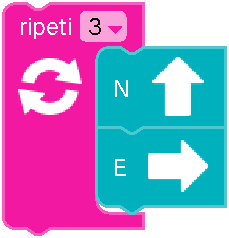
\includegraphics[scale=0.9]{img/codeorg-svg-cap07/pdf/codeorg-ripeti3ne.pdf}\label{credito:codeorg-labirinto-ripetizioni-2}}
\end{center}

\ruoliattivita{\ruoloEsecutore}

Per controllare che il blocco \textbf{ripeti} sia stato compreso, mostra uno alla volta i due programmi appena presentati e proponi questa consegna: ``Riscrivi il programma senza usare Ripeti. Quali istruzioni verranno eseguite, e in quale ordine? Disegna sul quaderno il percorso a partire da una casella che hai scelto''. In questa fase alunne e alunni assumono il ruolo di esecutori: devono interpretare un programma già scritto.


Chiedi di formulare la risposta prima della prova al computer, poi confrontatela con la figura seguente. Nel secondo caso si ripete tre volte l'intera sequenza di due istruzioni: Nord, Est, Nord, Est, Nord, Est.

\begin{center}
\begin{minipage}{0.94\linewidth}
\centering
\begin{minipage}[t]{0.47\linewidth}
\centering\vspace{0pt}
\textbf{Una sola istruzione ripetuta tre volte}\par\smallskip
\begin{tabular}{@{}c@{\hspace{0.4em}}c@{\hspace{0.4em}}c@{}}
\raisebox{-0.5\height}{
\includegraphics[scale=0.9]{img/codeorg-svg-cap07/pdf/codeorg-bozza-ripeti3n.pdf}\label{credito:codeorg-labirinto-ripetizioni-3}} &
$\Longleftrightarrow$ &
\raisebox{-0.5\height}{
\includegraphics[scale=0.9]{img/codeorg-svg-cap07/pdf/codeorg-bozza-sequenza3n.pdf}\label{credito:codeorg-labirinto-sequenze-1}}
\end{tabular}
\end{minipage}\hfill
\begin{minipage}[t]{0.47\linewidth}
\centering\vspace{0pt}
\textbf{Una sequenza di due istruzioni ripetuta tre volte}\par\smallskip
\begin{tabular}{@{}c@{\hspace{0.4em}}c@{\hspace{0.4em}}c@{}}
\raisebox{-0.5\height}{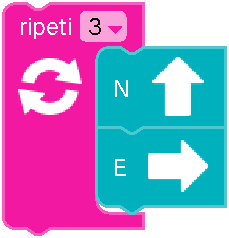
\includegraphics[scale=0.9]{img/codeorg-svg-cap07/pdf/codeorg-bozza-ripeti3ne.pdf}\label{credito:codeorg-labirinto-ripetizioni-4}} &
$\Longleftrightarrow$ &
\raisebox{-0.5\height}{
\includegraphics[scale=0.9]{img/codeorg-svg-cap07/pdf/codeorg-bozza-sequenza3ne.pdf}\label{credito:codeorg-labirinto-sequenze-2}}
\end{tabular}
\end{minipage}
\end{minipage}
\end{center}


\section{Attività 3: Artista (corsi A e B)}

\ruoliattivita{\ruoloProgrammatore}

La Lezione 10 del Corso A e la Lezione 9 del Corso B si svolgono nell'ambiente dell'Artista.

In questo tipo di livelli, si controlla un artista che, muovendosi sul foglio (esprimendo i movimenti sempre rispetto a un sistema di riferimento assoluto con i punti cardinali), potrà realizzare disegni geometrici.

La tabella seguente mostra l'effetto dei blocchi che alunni e alunne possono incontrare. Le direzioni restano sempre le stesse rispetto al foglio.

\begingroup
\manualeimpostazioni
\setlength{\LTleft}{0pt}
\setlength{\LTright}{0pt}
\arrayrulecolor{guideManualeBordo}
\begin{longtable}{|K{\dimexpr0.50\linewidth-2\tabcolsep-1.5\arrayrulewidth\relax}|J{\dimexpr0.50\linewidth-2\tabcolsep-1.5\arrayrulewidth\relax}|}
\hline
\manualetitolo{2}{ARTISTA A E B}
\manualeintestazione
\endfirsthead
\endhead
\multicolumn{2}{r@{}}{\small\itshape continua\ldots} \\
\endfoot
\endlastfoot
\manualeimmagini{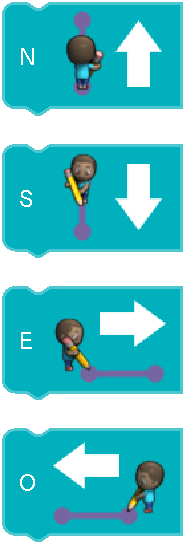
\includegraphics[scale=0.8]{img/codeorg-svg-cap07/pdf/codeorg-artista-nseo.pdf}\label{credito:codeorg-artista-direzioni-1}\hspace{6pt}%
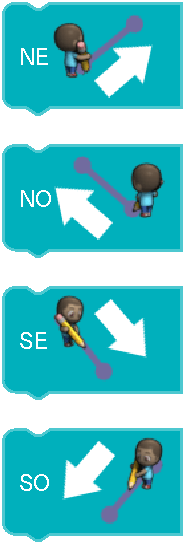
\includegraphics[scale=0.8]{img/codeorg-svg-cap07/pdf/codeorg-artista-diagonali.pdf}\label{credito:codeorg-artista-direzioni-2}}
& L'artista si muove e disegna un segmento nella direzione indicata, anche in diagonale.\par\medskip
\begin{center}
\begin{tikzpicture}[x=0.9cm,y=0.9cm,font=\sffamily\scriptsize]
  \draw[gray!50] (0,0) circle (0.8);
  \foreach \a in {0,45,...,315} \draw[line width=1.1pt,ocre,-stealth] (0,0) -- (\a:1.3);
  \node[font=\sffamily\scriptsize\bfseries] at (0,1.8) {NORD (N)};
  \node[font=\sffamily\scriptsize\bfseries] at (0,-1.8) {SUD (S)};
  \node[font=\sffamily\scriptsize\bfseries,anchor=west] at (1.5,0) {EST (E)};
  \node[font=\sffamily\scriptsize\bfseries,anchor=east] at (-1.5,0) {OVEST (O)};
  \node[anchor=south west,align=center] at (1.05,1.05) {NORD-EST\\(NE)};
  \node[anchor=south east,align=center] at (-1.05,1.05) {NORD-OVEST\\(NO)};
  \node[anchor=north east,align=center] at (-1.05,-1.05) {SUD-OVEST\\(SO)};
  \node[anchor=north west,align=center] at (1.05,-1.05) {SUD-EST\\(SE)};
\end{tikzpicture}
\end{center} \\
\hline
\manualeimmagini{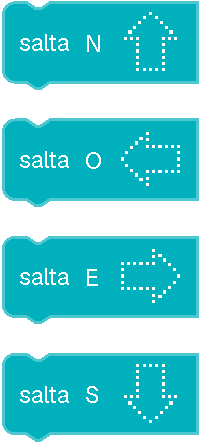
\includegraphics[scale=0.8]{img/codeorg-artista-cap07/pdf/codeorg-salta-cardinali.pdf}\label{credito:codeorg-artista-salti-1}\hspace{6pt}%
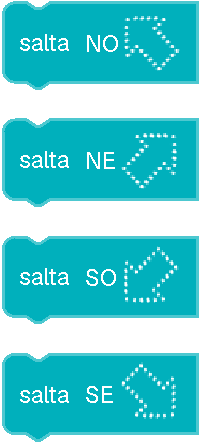
\includegraphics[scale=0.8]{img/codeorg-svg-cap07/pdf/codeorg-salta.pdf}\label{credito:codeorg-artista-salti-2}}
& L’artista si muove come nei blocchi sopra,
ma senza lasciare traccia. \\
\hline
\manualeimmagini{
\includegraphics[width=0.96\linewidth]{img/codeorg-artista-cap07/pdf/codeorg-imposta-schema.pdf}\label{credito:codeorg-artista-schema-1}\par\smallskip
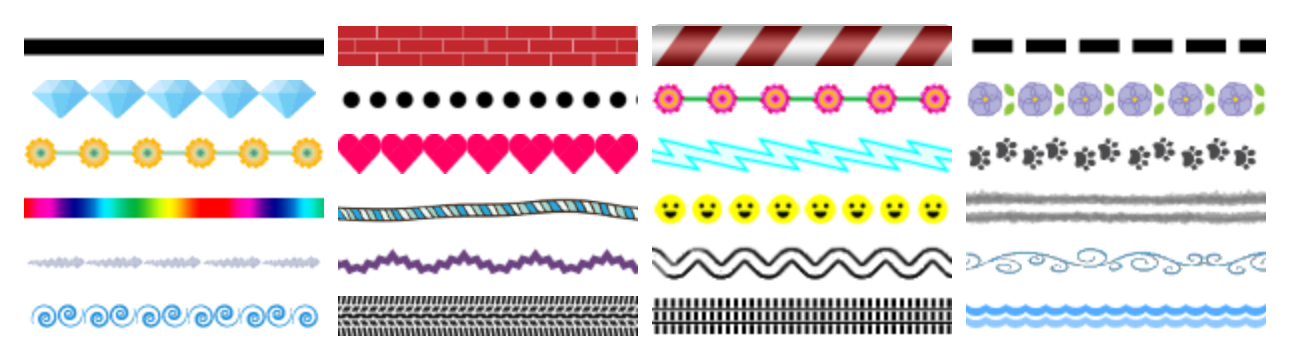
\includegraphics[width=0.96\linewidth]{img/codeorg-artista-schermate/schema-menu.png}\label{credito:codeorg-artista-menu-schema-1}}
& Da questa istruzione in poi, l'artista disegna usando lo schema scelto fra quelli proposti. Il menu permette di scegliere la trama del tratto. \\
\hline
\manualeimmagini{
\includegraphics[scale=0.85]{img/codeorg-svg-cap07/pdf/codeorg-imposta-colore.pdf}\label{credito:codeorg-artista-colore-1}}
& Da questa istruzione in poi, l'artista disegna usando una penna del colore scelto. \\
\hline
\manualeimmagini{
\includegraphics[scale=0.9]{img/codeorg-svg-cap07/pdf/codeorg-adesivo.pdf}\label{credito:codeorg-artista-adesivo-1}}
& L'artista stampa, nel punto in cui si trova, l'adesivo scelto, come un timbro. \\
\hline
\end{longtable}
\manualeripristinacolore
\endgroup

Si può cambiare la velocità con cui l'artista disegna: il disegno viene tracciato più lentamente quando il cursore è vicino alla tartaruga, più velocemente quando è vicino alla lepre. Rallentare l'esecuzione aiuta a osservare l'effetto di ogni istruzione.

\begin{center}
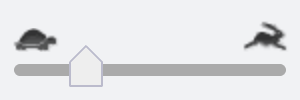
\includegraphics[width=5.5cm]{img/codeorg-artista-schermate/velocita.png}\label{credito:codeorg-artista-velocita-1}
\end{center}

\subsubsection{Leggere un programma e prevedere il disegno}

\ruoliattivita{\ruoloEsecutore}

Puoi proporre queste attività anche su un foglio quadrettato, senza computer o tablet. Mostra inizialmente soltanto il programma qui sotto, indica un punto di partenza e chiedi: ``Che cosa disegna l'artista se esegue queste istruzioni?''. Alunni e alunne assumono il ruolo di esecutori: leggono i blocchi dall'alto verso il basso e tracciano il percorso, mantenendo uguali i passi orizzontali e verticali.

Con il programma seguente, l'artista realizza una scaletta dall'alto in basso. Confronta il disegno ottenuto con la soluzione e, se possibile, fai verificare la previsione nell'ambiente Artista.

\begingroup
\setlength{\tabcolsep}{7pt}
\setlength{\arrayrulewidth}{0.4pt}
\arrayrulecolor{black!40}
\renewcommand{\arraystretch}{1.2}
\begin{center}
\begin{tabular}{|>{\centering\arraybackslash}m{\dimexpr0.50\linewidth-2\tabcolsep-1.5\arrayrulewidth\relax}|>{\centering\arraybackslash}m{\dimexpr0.50\linewidth-2\tabcolsep-1.5\arrayrulewidth\relax}|}
\hline
\rowcolor{black!12}
\sffamily\bfseries PROGRAMMA & \sffamily\bfseries SOLUZIONE \\
\hline
\vspace{5pt}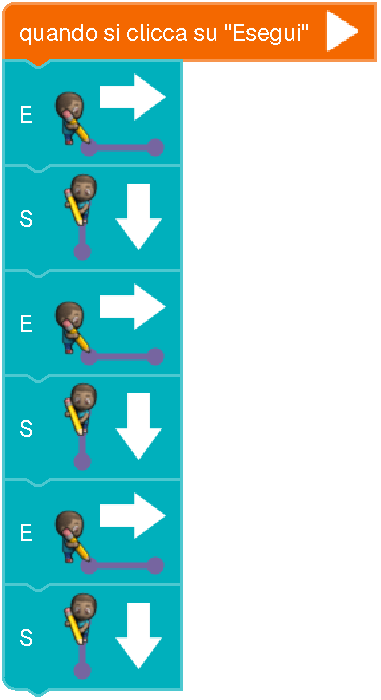
\includegraphics[scale=0.6]{img/codeorg-artista-cap07/pdf/codeorg-scala-programma.pdf}\label{credito:codeorg-artista-scaletta-programma-1}\par\vspace{5pt}
& \vspace{5pt}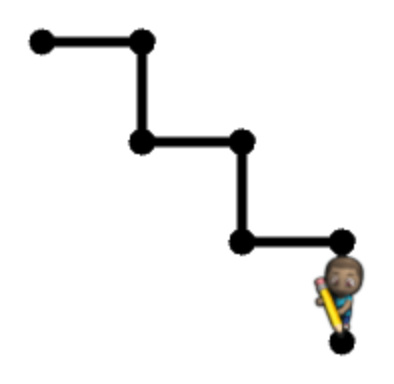
\includegraphics[width=0.85\linewidth]{img/codeorg-artista-schermate/scaletta.png}\label{credito:codeorg-artista-scaletta-disegno-1}\par\vspace{5pt} \\
\hline
\end{tabular}
\end{center}
\endgroup

\subsubsection{Scrivere un programma per un disegno}

Ora proponi il compito inverso (su carta o al computer): ``Aiuta l'artista a realizzare questi disegni''. Mostra soltanto i due disegni.

Di seguito sono riportate anche due possibili soluzioni.

\begin{center}
\begin{minipage}[t]{0.48\linewidth}
\centering\vspace{0pt}
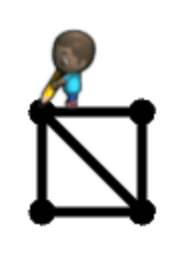
\includegraphics[height=3.3cm]{img/codeorg-artista-schermate/quadrato-diagonale.png}\label{credito:codeorg-artista-quadrato-diagonale-disegno-1}\par\medskip
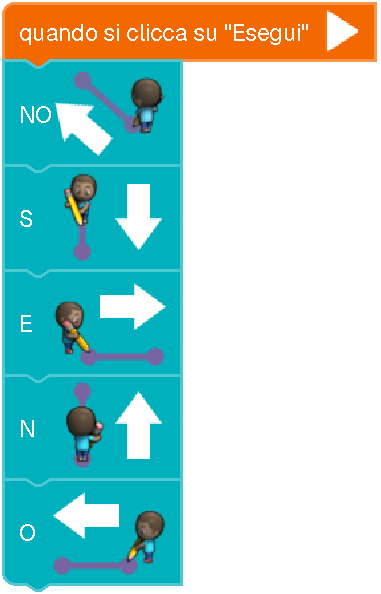
\includegraphics[scale=0.6]{img/codeorg-artista-cap07/pdf/codeorg-quadrato-diagonale-programma.pdf}\label{credito:codeorg-artista-quadrato-diagonale-programma-1}
\end{minipage}\hfill
\begin{minipage}[t]{0.48\linewidth}
\centering\vspace{0pt}

\includegraphics[height=3.3cm]{img/codeorg-artista-schermate/casa-strisce.png}\label{credito:codeorg-artista-casa-strisce-disegno-1}\par\medskip
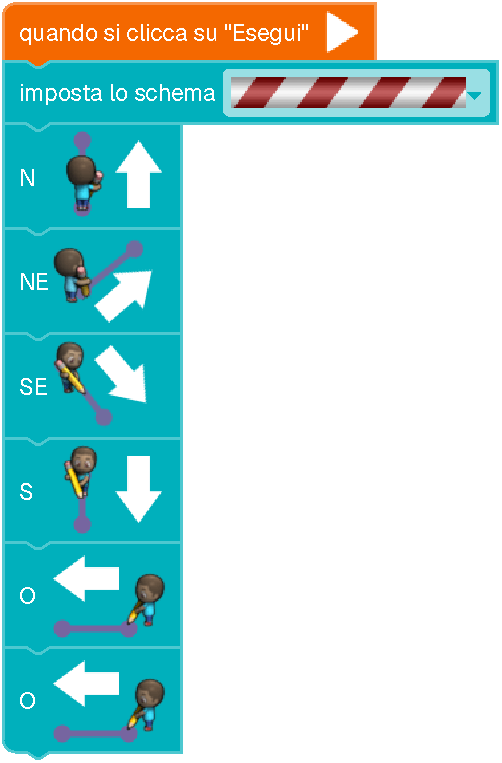
\includegraphics[scale=0.6]{img/codeorg-artista-cap07/pdf/codeorg-casa-schema-programma.pdf}\label{credito:codeorg-artista-casa-strisce-programma-1}
\end{minipage}
\end{center}

Per provare i programmi al computer, alunne e alunni possono usare il \textbf{Laboratorio Artista pre-scolare}: \linkbreve{artistaBase}. Qui alunni e alunne possono realizzare liberamente i propri disegni, senza un compito preassegnato.

Se qualcuno non sa cosa disegnare, ecco altri due suggerimenti che puoi dare loro (il secondo è più sfidante).

\begin{center}
\begin{minipage}[t]{0.48\linewidth}
\centering\vspace{0pt}
\parbox[c][3.2cm][c]{\linewidth}{\centering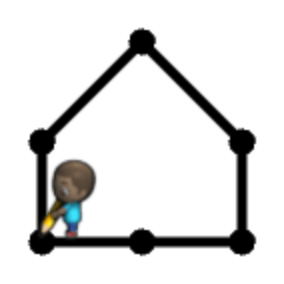
\includegraphics[height=3.2cm]{img/codeorg-artista-schermate/casa.png}\label{credito:codeorg-artista-casa-disegno-1}}\par\medskip
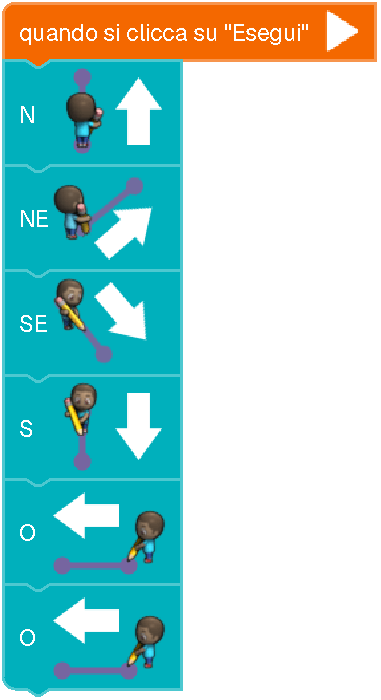
\includegraphics[scale=0.5]{img/codeorg-artista-cap07/pdf/codeorg-casa-programma.pdf}\label{credito:codeorg-artista-casa-programma-1}
\end{minipage}\hfill
\begin{minipage}[t]{0.48\linewidth}
\centering\vspace{0pt}
\parbox[c][3.2cm][c]{\linewidth}{\centering
\includegraphics[width=\linewidth]{img/codeorg-artista-schermate/trama.png}\label{credito:codeorg-artista-trama-disegno-1}}\par\medskip
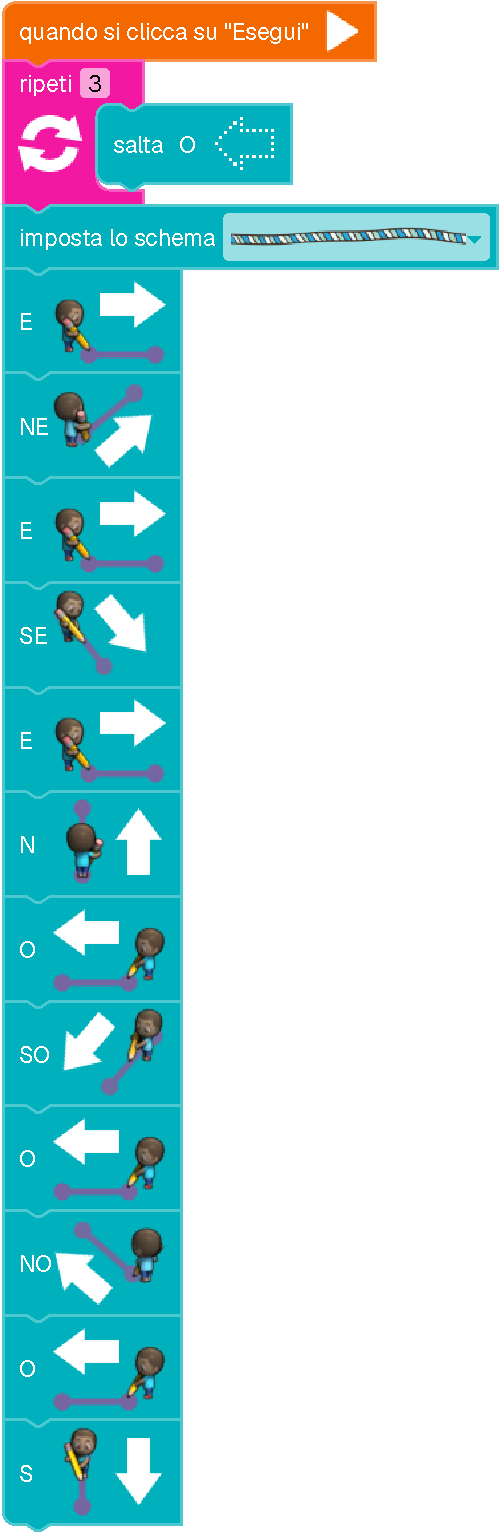
\includegraphics[scale=0.5]{img/codeorg-svg-cap07/pdf/codeorg-trama-ripetuta-programma.pdf}\label{credito:codeorg-artista-trama-programma-1}
\end{minipage}
\end{center}


\section{Attività 4: Labirinti (corso C)}

\ruoliattivita{\ruoloProgrammatore}

Le Lezioni 3, 4, 5, 8, 9 del Corso C sono tutte collocate nell'ambiente ``Labirinti''. L'ambiente è del tutto analogo a quelli dei Corsi A e B, ma, da questo corso in poi, i movimenti del personaggio saranno descritti rispetto a un sistema di riferimento soggettivo centrato sul personaggio, così come abbiamo visto nelle attività unplugged con riferimenti soggettivi (vedere Capitolo~\ref{capitolo-4-movimenti-su-una-griglia} - Movimenti sulla griglia).

Quindi, in questa attività, chi programma vive la scena dal punto di vista del personaggio: quando c'è un'istruzione di movimento, è sempre ``rispetto a dove sta guardando il personaggio''. Se dici al personaggio ``vai avanti'', lui cammina nella direzione in cui è rivolto il suo sguardo.




\section{Altre attività }\label{altre-attivituxe0}

\ruoliattivita{\ruoloProgrammatore}

\subsection{Eventi (corsi A, B, C) }\label{eventi-corsi-a-b-c}

Nella Lezione 12 del Corso A e del Corso B, e nelle lezioni 12, 13 e 16 del Corso C è possibile costruire videogiochi, storie e animazioni facendo parlare personaggi, facendoli muovere e facendoli reagire ad eventi (es. click del mouse, pressione dei tasti freccia sulla tastiera).

Lascia che studenti e studentesse sperimentino con questi livelli. L'introduzione alla creazione di giochi, storie, animazioni è la parte centrale di Scratch, che verrà introdotto nel prossimo capitolo.

\subsection{Artista (corso C) }\label{artista-corso-c}

Nel Corso C, anche nei livelli dedicati all'artista i movimenti vengono espressi rispetto a un sistema di riferimento soggettivo, centrato sull'Artista, ed è presente anche la possibilità di orientarlo di un certo angolo. Puoi lasciare che i tuoi studenti sperimentino intuitivamente e poi, al momento opportuno, collegare quanto emerso dalle loro esplorazioni ai concetti geometrici più formali.


\subsubsection{Lunghezze e angoli nell'Artista}

\ruoliattivita{\ruoloProgrammatore\quad\ruoloEsecutore}

Nell'Artista del Corso C puoi rendere concreto il significato dei numeri presenti nei blocchi.

\begin{center}
\manualeimpostazioni
\begin{tabular}{|K{\dimexpr0.50\linewidth-2\tabcolsep-3\arrayrulewidth/2\relax}|J{\dimexpr0.50\linewidth-2\tabcolsep-3\arrayrulewidth/2\relax}|}
\arrayrulecolor{guideManualeBordo}
\hline
\manualetitolo{2}{ARTISTA CORSO C}
\manualeintestazione
\manualeimmagini{
\includegraphics[scale=0.9]{img/codeorg-svg-cap07/pdf/codeorg-bozza-artista-avanti100.pdf}\label{credito:codeorg-artista-comandi-angoli-1}}
& Fa avanzare l'artista nella direzione in cui guarda e traccia un tratto rettilineo lungo 100 pixel. Il pixel, già incontrato parlando di immagini digitali (vedi~\ref{rappresentare-colori-immagini-video}), viene qui usato come unità per esprimere la lunghezza sullo schermo. \\
\hline
\manualeimmagini{
\includegraphics[scale=0.9]{img/codeorg-svg-cap07/pdf/codeorg-bozza-artista-destra90.pdf}\label{credito:codeorg-artista-comandi-angoli-2}}
& Fa ruotare l'artista su se stesso di 90° verso destra e senza tracciare un nuovo tratto rettilineo. \\
\hline
\end{tabular}
\manualeripristinacolore
\end{center}

Ad esempio, si può proporre di cambiare l'ampiezza in gradi dell'angolo di rotazione impostando valori come 45, 60, 90 o 120 gradi (o cambiando il verso) e poi confrontare la direzione finale con quella iniziale. È importante notare che il valore numerico nel blocco indica l'ampiezza dell'angolo di rotazione rispetto alla direzione attuale dell'artista (quindi non, ad esempio, l'angolo interno della figura che si sta disegnando). Prima di eseguire il programma, può essere utile chiedere di indicare con la mano da quale parte sarà rivolto l'artista per poi confrontare la previsione con il risultato.




\begin{center}
\begin{minipage}{0.94\linewidth}
\centering
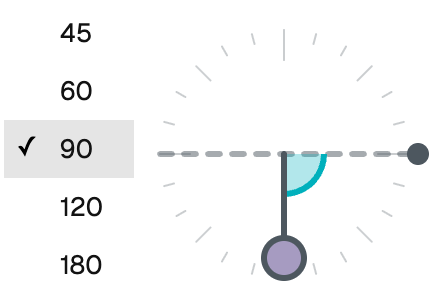
\includegraphics[width=4.2cm]{img/codeorg-artista-schermate/menu-angoli.png}\label{credito:codeorg-artista-selettore-angoli-1}
\par\smallskip
\textbf{Scegliere l'angolo di rotazione}\par
\end{minipage}
\end{center}

\begin{center}
\begin{minipage}{0.94\linewidth}
\centering
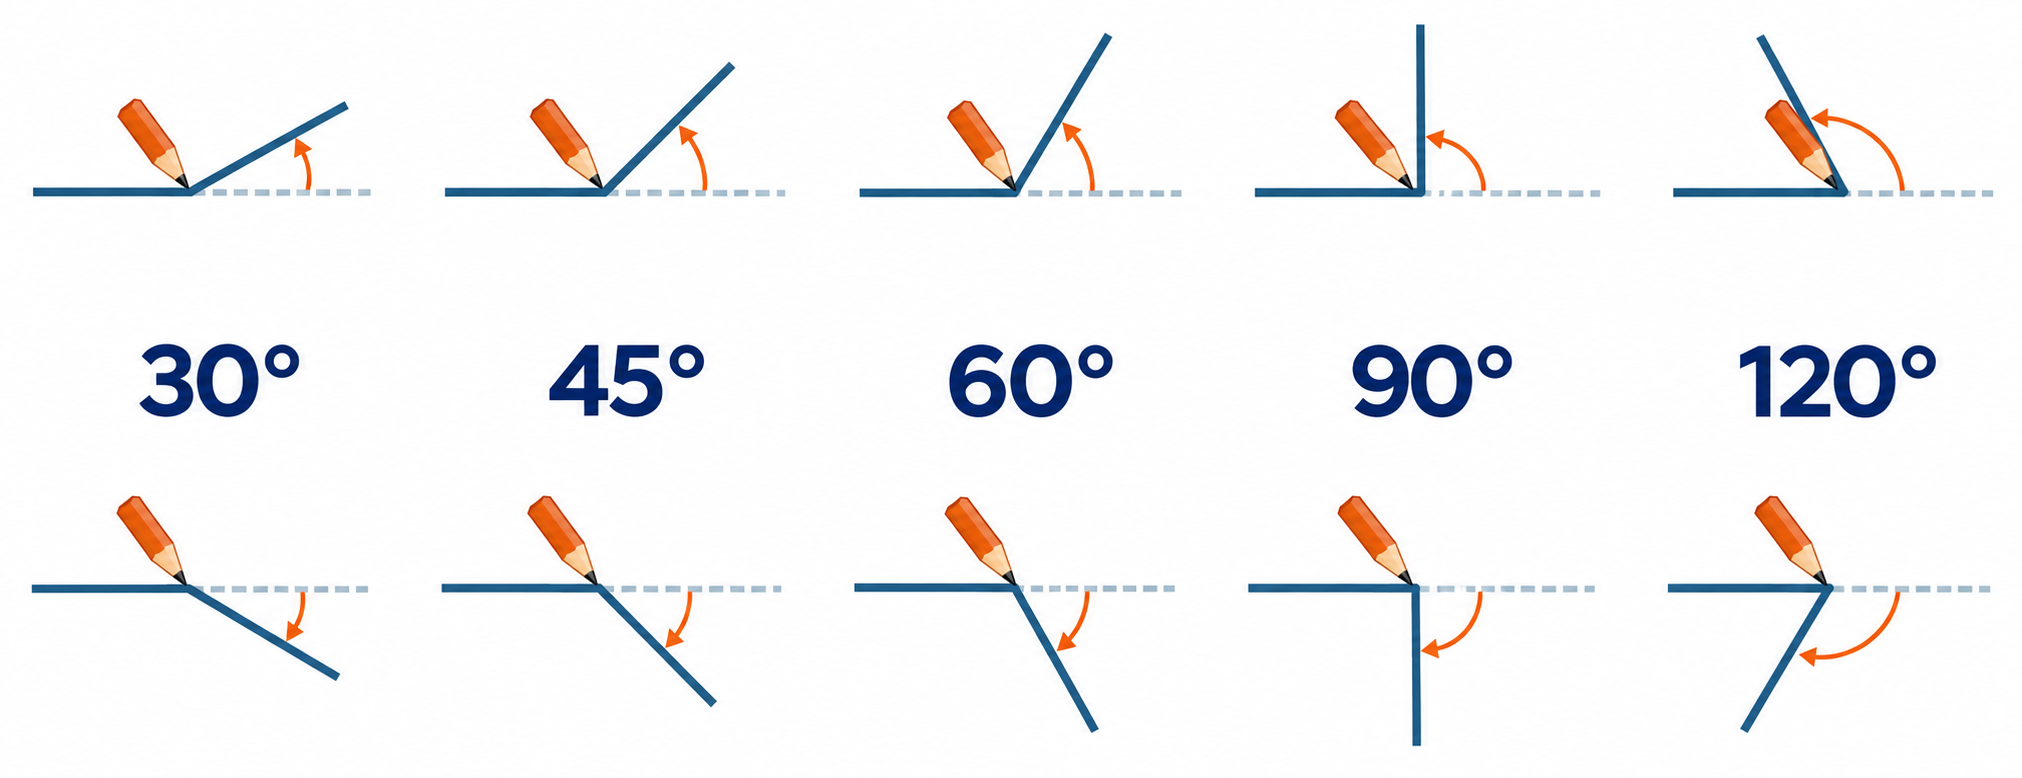
\includegraphics[width=\linewidth]{img/rotazioni-matita.png}\label{credito:rotazioni-matita-1}
\par\smallskip
\textbf{Confrontare le rotazioni.} Da una stessa direzione iniziale, gli esempi mostrano rotazioni di 30, 45, 60, 90 e 120 gradi verso sinistra (sopra) e verso destra (sotto). La linea tratteggiata prolunga la direzione precedente.\par
\end{minipage}
\end{center}

Combinando segmenti e rotazioni si possono costruire anche figure riconoscibili, come questo gattino. Puoi usarlo come spunto per chiedere di individuare le parti del disegno e immaginare quali movimenti permettano di realizzarle; lascia poi che ciascuno inventi una propria figura.

\begin{center}
\begin{minipage}{0.94\linewidth}
\centering

\includegraphics[width=5.2cm]{img/gattino-matita/gattino.pdf}\label{credito:gattino-matita-1}
\end{minipage}
\end{center}

Per continuare a disegnare senza un compito preassegnato, puoi aprire il \textbf{laboratorio libero dell'Artista}: \linkbreve{artista}. È l'ambiente con lunghezze e angoli nei blocchi, distinto dal Laboratorio Artista pre-scolare già usato per i corsi A e B.

\subsection{L'Ora dell'InformaticA (l'Ora del Codice) }\label{lora-dellinformatica-lora-del-codice}

Code.org è diventata famosa per l'iniziativa ``L'ora del Codice'', dal 2025 rinominata ``L'ora dell'InformaticA'' (per maggiormente rimarcare da un lato l'aspetto disciplinare, e dall'altro l'introduzione di elementi di Intelligenza Artificiale). Si tratta di un'iniziativa in cui, più o meno nello stesso periodo (es. la ``Settimana Internazionale dell'Insegnamento dell'Informatica'', che solitamente cade a dicembre - \urloriginale{https://www.csedweek.org/}), le bambine e i bambini di tutto il mondo svolgono almeno un'ora di introduzione alla programmazione. Puoi consultare le attività proposte sul sito: \linkbreve{oraInformaticA}.

\section{Modalità di lavoro }\label{modalituxe0-di-lavoro-4}

L'approccio guidato dalla piattaforma dovrebbe permettervi di far sì che, una volta avviata l'attività, studenti e studentesse procedano in modo autonomo e ciascuno al proprio ritmo. Tuttavia, è importante facilitare e vigilare costantemente sul processo.

\subsection{Debugging }\label{debugging}

Le attività proposte in questo capitolo della guida offrono un contesto autentico per sperimentare la pratica del debugging. Infatti, se escludiamo le attività con i robot educativi, questa è probabilmente la prima volta che gli studenti hanno a che fare realmente con un esecutore automatico, ``meccanico''.

Come abbiamo visto, in informatica, più che applicare una procedura già nota, si tratta spesso di progettarne una che risolva il problema in questione, ma non sia già conosciuta e che, idealmente, possa funzionare anche per altri casi simili appartenenti alla stessa classe di problemi. Sarà quindi normale procedere, almeno in parte, con prove ed errori. Se da un lato all'inizio può essere frustrante vedere che il programma non fa ciò che ci si aspetta, dall'altro--una volta convinti studenti e studentesse che il computer esegue sempre e solo la sequenza di istruzioni che gli vengono date, e in modo sempre ``prevedibile'' e ``ripetibile''--si può accettare più serenamente che l'errore è dovuto a un programma che va rivisto e migliorato perché non aderente agli obiettivi.

Per abituare studenti e studentesse a riconoscere le cause degli errori e correggerli, può essere utile aiutarli a strutturare le fasi di debug, ad esempio proponendo di seguire le fasi spiegate nel box che segue.

\subsubsection{Fasi di debugging}

\begin{enumerate}
\def\labelenumi{\arabic{enumi}.}
\item
  Assicurarsi di aver capito qual è l'obiettivo del protagonista.
\item
  Eseguire il programma: cosa c'è di sbagliato nel comportamento del protagonista?
\item
  Cercare di determinare quali blocchi sono responsabili del comportamento sbagliato (per capirlo meglio può essere utile usare ``Fai un passo'' per eseguire un'istruzione alla volta, vedendo che effetto ha sul programma; oppure far disegnare l'Artista più lentamente).
\item
  Modificare il programma (aggiungere o togliere istruzioni, o modificare i numeri presenti in esse) e poi rieseguirlo.
\item
  Se ancora non funziona, valutare se con le modifiche fatte ci si sta avvicinando all'obiettivo oppure se è meglio annullarle.
\item
  Ritornare al passo 3 fino a che non si è raggiunto l'obiettivo.
\end{enumerate}

\subsection{Programmazione in coppia }\label{programmazione-in-coppia}

Un altro modo di fare debugging è raccontare a un compagno o una compagna che cosa fa il proprio programma. Spesso il solo fatto di spiegare ad alta voce le istruzioni del proprio programma fa capire a chi l'ha creato dove ha sbagliato. Nell'industria informatica, questa pratica è stata istituzionalizzata come metodologia chiamata ``pair programming'', cioè ``programmazione in coppia'' - due programmatori programmano insieme su un solo computer. È una metodologia estremamente utile anche a scuola.

Nella programmazione in coppia, pensiamo la coppia come a un equipaggio da rally: da una parte c'è il \textbf{pilota}, dall'altra il \textbf{navigatore}. Come in un vero rally, il pilota ha in mano il ``volante'', cioè il mouse: il pilota materialmente guida il programma, clicca, trascina i blocchi, scrive il codice. Il suo obiettivo è arrivare a un programma funzionante, proprio come il pilota vuole portare l'auto al traguardo. Mentre lavora, però, non lo fa in silenzio: il pilota racconta ad alta voce al navigatore che cosa sta facendo, passo dopo passo, spiegando perché sceglie un certo blocco o lo mette in un certo punto. Il compagno o la compagna con il ruolo di navigatore potrà dare dei suggerimenti ma alla fine sarà il pilota a prendere le decisioni finali: ha il volante/mouse in mano.

Il navigatore, invece, è come il copilota nel rally: osserva con attenzione ciò che fa il pilota e ascolta ciò che dice, ma non tiene il volante. Il suo compito è guardare bene la ``strada'' che hanno davanti, in questo caso il puzzle di programmazione, e aiutare il pilota a non perdersi. Può notare errori, proporre correzioni, suggerire strade alternative: ``E se invece provassimo a mettere questo blocco qui?'', ``Secondo me così il personaggio non arriverà dove vogliamo''. Mentre il pilota si concentra sui dettagli, il navigatore mantiene la visione d'insieme: verifica se il programma sta davvero procedendo nella direzione giusta per risolvere il problema.

Ogni tanto si scambiano i ruoli: chi guidava diventa il navigatore e chi faceva il navigatore passa al volante. All'inizio sarà l'insegnante a guidare questo scambio e a ricordare i compiti di ciascuno, ma l'obiettivo è che studenti e studentesse imparino pian piano a collaborare in modo autonomo.

Come insegnante dovrai fare attenzione nel formare (e, se necessario, separare) le coppie e, soprattutto, nel far rispettare i ruoli: un pilota che non considera il navigatore o un navigatore prepotente sono da evitare!

In questo video viene spiegata la metodologia: \linkbreve{coppia}.

Su Code.org è possibile cliccare sulla casella accanto alla scritta ``Sto lavorando in coppia'' che appare una volta effettuato il login, quindi cliccare prima sul nome del compagno o della compagna con cui si sta lavorando e poi sul pulsante ``Aggiungi partner'', per essere sicuri che vengano tracciati i progressi di entrambi i membri della coppia (o anche di gruppi più numerosi).

\subsection{Evitare l'effetto ``basta superare il livello'' }\label{evitare-leffetto-basta-superare-il-livello}

La modalità con cui progrediscono le lezioni di Code.org (piccoli puzzle da superare) dovrebbe essere congeniale perché studenti e studentesse li considereranno livelli da superare in un videogioco. Tuttavia, è importante evitare che questo generi l'idea che basti ``far venire gli esercizi'' (senza aver capito perché la soluzione proposta è corretta, oppure proponendo soluzioni molto lunghe e ripetitive da scrivere), magari addirittura gareggiando per chi li completa prima. Di seguito discutiamo alcune strategie per superare questo approccio ingenuo.


\subsection{Esistono più programmi corretti!}


Uno degli aspetti più belli dell'informatica è che lo stesso problema può avere molte soluzioni diverse, tutte valide. In Code.org, questo diventa subito evidente: programmi differenti possono portare il personaggio allo stesso obiettivo, pur utilizzando blocchi o strategie non identiche. È importante valorizzare questo aspetto: non si tratta di trovare ``la'' risposta giusta, ma di scoprire che esistono modi diversi per arrivare allo stesso risultato! Questa varietà permette attività ricchissime in classe:

\begin{itemize}
\item
  confrontare soluzioni diverse;
\item
  raccontare come ciascuno ha ragionato;
\item
  osservare cosa cambia se si sposta un blocco;
\item
  scoprire nuove idee guardando il lavoro degli altri.
\end{itemize}

In questo modo la programmazione diventa un terreno di dialogo e creatività: ogni soluzione è un punto di vista, e il confronto tra programmi aiuta a capire meglio sia il problema sia i concetti informatici in gioco.

\subsection{La sfida è usare meno blocchi possibile }\label{la-sfida-uxe8-usare-meno-blocchi-possibile}

Nell'Area di lavoro viene sempre indicato il numero di blocchi attualmente utilizzati nel programma. Solitamente, se si risolve un puzzle usando un numero elevato di blocchi, Code.org suggerisce che sarebbe stato possibile farlo con meno. È importante che, piano piano, studenti e studentesse comincino ad apprezzare programmi che fanno uso di meno blocchi, in quanto più chiari e semplici da comprendere (e anche da realizzare, ad esempio, senza dover trascinare lunghe sequenze di blocchi tutti uguali). Dunque, è importante suggerire di non superare il numero di blocchi indicato come obiettivo nel titolo dell'Area di lavoro.

L'esempio del blocco Ripeti è lampante: non è necessario per risolvere i semplici problemi proposti in questi corsi, ma consente di realizzare programmi decisamente più brevi (cioè con meno blocchi) e quindi più leggibili.

\begin{center}
\begingroup
\setlength{\tabcolsep}{5pt}
\setlength{\arrayrulewidth}{0.4pt}
\arrayrulecolor{black!40}
\renewcommand{\arraystretch}{1.15}
\begin{tabular}{|c|c|c|}
\hline
\begin{minipage}[c]{\dimexpr0.30\linewidth-2\tabcolsep-4\arrayrulewidth/3\relax}\centering\vspace{5pt}
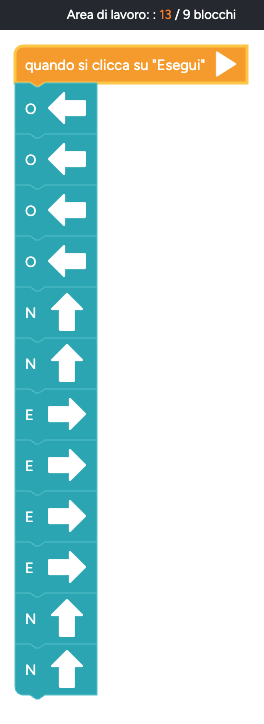
\includegraphics[width=0.988764\linewidth]{img/codeorg-confronto-blocchi/programma-13.png}\label{credito:codeorg-confronto-13-9-1}\par\vspace{5pt}
\end{minipage}
& \begin{minipage}[c]{\dimexpr0.40\linewidth-2\tabcolsep-4\arrayrulewidth/3\relax}\raggedright
Ad esempio, il programma di sinistra usa 13 blocchi ma se ne poteva realizzare un altro con lo stesso effetto usando solo 9 blocchi (immagine a destra)!
\end{minipage}
& \begin{minipage}[c]{\dimexpr0.30\linewidth-2\tabcolsep-4\arrayrulewidth/3\relax}\centering\vspace{5pt}
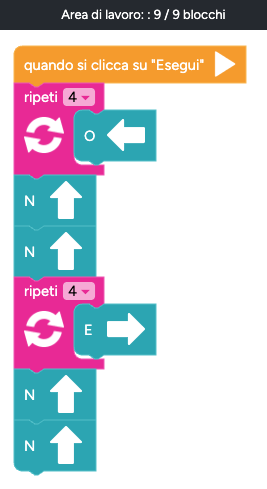
\includegraphics[width=\linewidth]{img/codeorg-confronto-blocchi/programma-9.png}\label{credito:codeorg-confronto-13-9-2}\par\vspace{5pt}
\end{minipage} \\
\hline
\end{tabular}
\endgroup
\end{center}

\bigskip

A volte compare un numero rosso che indica il numero massimo di volte in cui si può usare un blocco nel programma.


\begin{center}

\includegraphics[width=2.8cm]{img/codeorg-confronto-blocchi/codeorg-est-limite-1.pdf}\label{credito:codeorg-est-limite-1}
\end{center}


Questo è un altro modo su Code.org per ``forzare'' alunne e alunni a utilizzare, ad esempio, il blocco Ripeti.

\section{Valore costruzionista }\label{valore-costruzionista-4}

Da un punto di vista metodologico, in Code.org la scoperta di nuovi concetti è inizialmente molto vincolata da un elevato scaffolding, cioè un insieme di \emph{sostegni temporanei} che aiutano bambini e bambine a procedere passo passo fino a diventare autonomi. Pian piano viene concessa loro maggiore libertà creativa \parencite{resnick-rusk-2020}. Tuttavia, in ogni puzzle da risolvere viene spesso richiesto di usare nuovi blocchi lasciando a studenti e studentesse la possibilità di esplorarne il funzionamento per capire come utilizzarli per raggiungere gli obiettivi e superare i livelli.

Per poter aumentare la libertà di esplorazione anche quando si programma su Code.org è nato, in direzione costruzionista, l'approccio metodologico chiamato \emph{Usa-Modifica-Crea}, che descriviamo di seguito.

\subsection{Usa, Modifica, Crea }\label{usa-modifica-crea}

In questo approccio metodologico (o meglio, famiglia di approcci metodologici - poiché è stato declinato in molti modi diversi), studenti e studentesse imparano usando programmi già scritti, modificandoli e, infine, creando programmi tutti loro.

Le attività sono solitamente organizzate in tre fasi. Le fasi hanno un ordine logico, ma non sono rigide: si può andare avanti o indietro più volte.

Le descriviamo di seguito, affidandoci a \AtNextCite{\defcounter{maxnames}{99}}\textcite{caserio-etal-umc}.

\begin{enumerate}
\item
  Fase ``\textbf{Usa}'': ``Provo il programma degli altri''

In questa prima fase si esegue un programma già pronto, costruito dall'insegnante o da altri, rispondendo poi a domande di riflessione.


\begin{itemize}
\item
  Il programma non è banale: deve essere un po' ``curioso'' o ``bello da vedere'' (es. un minigioco o una storia autoconclusiva) e, idealmente, contenere i nuovi concetti che si vogliono introdurre.
\item
  Bambini e bambine eseguono il programma senza vedere le istruzioni di cui è composto: osservano semplicemente ciò che succede sullo schermo, e rispondono a domande di riflessione su ciò che hanno esperito. In questo modo studenti e studentesse si concentrano prima sul descrivere e interpretare il comportamento del programma e non sulle istruzioni.
\end{itemize}

\item
  Fase ``\textbf{Modifica}'': ``Metto mano al codice''

Nella seconda fase, studenti e studentesse possono vedere le istruzioni che costituiscono il programma. L'obiettivo è leggere le istruzioni (i blocchi), esplorarli e collegarli a ciò che accade sullo schermo quando il programma viene eseguito. L'insegnante in questa fase può proporre vari tipi di attività, quali:

\begin{itemize}
\item
  Richiedere di apportare modifiche alle istruzioni del programma, come ad esempio spostare o sostituire un blocco, o cambiare un numero dentro a un blocco. Studenti e studentesse eseguiranno quindi di nuovo il programma osservando che cosa è cambiato nell'effetto.
\item
  Richiedere di fare previsioni. Prima di apportare la modifica, l'insegnante invita studenti e studentesse a formulare esplicitamente un'ipotesi sull'effetto che avrà la modifica sul risultato dell'esecuzione del programma. Solo dopo che ciascuno avrà formulato la propria previsione si potrà procedere con la modifica del programma, confrontando le varie ipotesi con il risultato.
\item
  Richiedere di apportare modifiche alle istruzioni del programma con un obiettivo dato. Viene dato un obiettivo esplicito e circoscritto, per esempio: cambiare un dettaglio grafico; variare in piccola parte il funzionamento del programma. Studenti e studentesse quindi proveranno, sbaglieranno, ritenteranno finché non raggiungono il risultato richiesto.
\end{itemize}


In questa fase si lavora molto sulla curiosità e sulla sperimentazione, orientando sempre le attività di modifica a comprendere meglio i nuovi concetti da introdurre.


\item
  Fase ``\textbf{Crea}'': ``Costruisco il mio programma''


Nella terza fase, studenti e studentesse sono invitati a creare un proprio programma personale, utilizzando anche i nuovi concetti appresi. La creazione può essere più o meno dirompente rispetto ai progetti delle fasi precedenti.


\begin{itemize}
\item
  Creazione come evoluzione delle modifiche. Studenti e studentesse partono dal programma proposto dall'insegnante, ma decidono di modificare in modo più profondo la grafica o il funzionamento. Il tuo ruolo di insegnante in questo caso sarà quello di controllare che, nelle loro creazioni, studenti e studentesse utilizzino i nuovi concetti introdotti.
\item
  Creazione libera con alcuni vincoli. Studenti e studentesse possono progettare un programma anche molto diverso da quelli visti prima, ma con qualche vincolo chiaro, ad esempio: usare alcuni blocchi obbligatori; rispettare un certo comportamento generale dei personaggi.
\end{itemize}

\end{enumerate}

In questo modo, anche nella creazione più libera, bambini e bambine devono comunque mettere in gioco i nuovi concetti, consolidandoli attraverso le proprie idee.


\textbf{Un esempio di materiale didattico completo} (che comprende sia le schede studenti che una guida passo-passo per l'insegnante) per introdurre il concetto di ciclo utilizzando l'Artista di Code.org in una classe di terza primaria è disponibile all'indirizzo: \urloriginale{https://lodi.ml/umc}.

\section{Aspetti informatici }\label{aspetti-informatici-3}

In queste attività studenti e studentesse incontrano per la prima volta un vero linguaggio di programmazione. È fatto di blocchetti colorati, ma ha tutte le caratteristiche di un linguaggio formale: ad esempio, ha una sintassi (i blocchetti si incastrano solo in un certo modo) e una semantica (es. la sequenza di istruzioni incluse nella forma a C di un Ripeti viene eseguita il numero di volte indicato nel blocco stesso).

In queste attività studenti e studentesse non si limitano a ``giocare con i blocchi'', ma incontrano alcune idee chiave di informatica.

\begin{itemize}
\item
  \textbf{Algoritmo vs programma}. I puzzle dei Labirinti e dell'Artista rendono visibile il passaggio dall'algoritmo (la sequenza di istruzioni pensata a voce o su carta) al programma (cioè l'algoritmo tradotto in un linguaggio di programmazione eseguibile dal computer). La stessa strategia usata negli esercizi unplugged (sequenze di frecce o istruzioni) deve ora essere tradotta in blocchi, rispettando la sintassi del linguaggio.
\item
  \textbf{Sequenza e ciclo come prime strutture di controllo}. La maggior parte dei puzzle può essere risolta con semplici sequenze; l'introduzione del blocco Ripeti permette di ``compattare'' programmi lunghi e ripetitivi, facendo emergere l'idea che un buon programma non è solo quello che ``funziona'', ma anche quello più leggibile e manutenibile (quindi ad esempio ha meno blocchi ed è più chiaro).
\item
  \textbf{Parametri e generalizzazione}. Nei livelli dell'Artista, trovi alcuni blocchi che richiedono di specificare dei numeri. In informatica, questi numeri sono chiamati parametri: indicano quanto deve muoversi o ruotare l'Artista. Cambiando il parametro, puoi ottenere disegni diversi: non stai più programmando ``questo quadrato preciso'', ma stai programmando ``un quadrato di lato di lunghezza x'', semplicemente modificando il numero. È una prima forma di generalizzazione, perché studenti e studentesse capiscono che un programma può funzionare anche quando cambiano i valori.
\item
  \textbf{Esecutore meccanico}. Il personaggio sullo schermo si comporta come un esecutore ``ottuso'': fa esattamente ciò che c'è scritto nel programma, né più né meno. Insistere su questo aspetto aiuta studenti e studentesse a costruirsi una prima immagine mentale del calcolatore come sistema deterministico che esegue alla lettera una sequenza di istruzioni.
\item
  \textbf{Previsione, esecuzione e debugging.} In questo capitolo, nella sezione relativa alla Modalità di lavoro, il debugging è già stato presentato come pratica centrale per accogliere e affrontare gli errori in modo sereno e sistematico. In questo modo studenti e studentesse imparano che l'errore non è un fallimento, ma un'informazione preziosa sul funzionamento del proprio programma.
\end{itemize}

\section{Relazione con l'informatica nelle Indicazioni Nazionali 2025 }\label{relazione-con-linformatica-nelle-indicazioni-nazionali-4}

Relativamente alle Indicazioni Nazionali 2025, queste attività contribuiscono allo sviluppo delle seguenti competenze, obiettivi e conoscenze (queste ultime inserite nelle Indicazioni Nazionali 2025 a titolo di esempio, non prescrittive).


\subsubsection{Competenze (alla fine della scuola primaria) nella disciplina Matematica}


\begin{itemize}
\item
  \emph{Scrivere e comprendere semplici programmi, espressi in elementari linguaggi di programmazione a scopo didattico, e valutarne l'adeguatezza rispetto al compito che si vuole automatizzare.}
\end{itemize}



\subsubsection{Obiettivi (alla fine della terza primaria) nella disciplina Matematica}


\begin{itemize}
\item
  \emph{Scrivere semplici programmi e verificare, mediante la loro esecuzione, se svolgono il compito previsto ed eventualmente correggerli.}
\end{itemize}


\subsubsection{Obiettivi (alla fine della terza primaria) nella disciplina Tecnologia}


\begin{itemize}
\item
  \emph{Creare, selezionare e usare semplici testi o disegni, usando strumenti informatici.}
\end{itemize}

\subsubsection{Conoscenze (scuola primaria) nella disciplina Matematica}

\begin{itemize}
\item
  \emph{Concetto di algoritmo e sua esecuzione rigorosa.} In particolare qui si lavora sulla creazione ed esecuzione di programmi, cioè algoritmi scritti in un linguaggio di programmazione (qui, in particolare, il linguaggio a blocchi di Code.org).
\item
  \emph{Strutture di controllo fondamentali di un linguaggio di programmazione e reazione agli eventi.}
\item
  \emph{Controllo di correttezza dei programmi.}
\end{itemize}

\section{Suggerimenti per ulteriori attività}\label{suggerimenti-per-ulteriori-attivituxe0-e-riferimenti-4}

\printbibliography[heading=none,keyword={cap7},category={attivita}]

\begin{rimandiquaderno}
Se possiedi il volume studente \emph{Sulle orme di Milù -- Informatica}
(Mondadori Education, 2026), puoi usare i rimandi seguenti per affiancarlo
alle attività di questo capitolo.\par\smallskip

\begin{itemize}[leftmargin=*,itemsep=5pt,topsep=4pt]
\item \textbf{Introduzione a Code.org (Attività 1).} Alle pagg.~28--29, le schede BENVENUTI IN CODE.ORG accompagnano i primi passi negli ambienti guidati dei corsi di Introduzione all'Informatica.
\item \textbf{Labirinti (Attività 2).} Le schede LABIRINTI~\textbullet{}~2 (pagg.~30--31) si collegano alle lezioni nell'ambiente Labirinti dei corsi A e B e comprendono una guida sintetica all'effetto dei blocchi-direzione. Se mancano computer o tablet, oppure per assegnare un compito unplugged, la scheda IL VIAGGIO DEL POLPO (pag.~31) propone su carta lo stesso esercizio online: l'ambientazione cambia, ma le soluzioni restano le stesse. \textbf{Soluzione:} N, E, E, E, S. \textbf{Sfida finale con soli 4 blocchi:} N, ripeti 3 volte [E], S. Un'attività identica, con solo ambientazione diversa, online, è disponibile a  \linkbreve{codeLabirinto}. (NB: il blocco “quando si clicca su “Esegui”” non è presente né conteggiato nel
Quaderno di Informatica, mentre è conteggiato su Code.org).
\item \textbf{Artista (Attività 3).} Le schede ARTISTA (pagg.~32--33) corrispondono alle attività nell'ambiente Artista dei corsi A e B; a pag.~32 è presente anche una guida sintetica all'effetto dei blocchi.
\item \textbf{Labirinti (Attività 4).} Le schede LABIRINTI~\textbullet{}~3 (pagg.~34--35) si collegano alle lezioni nell'ambiente Labirinti del Corso C e comprendono una guida sintetica ai blocchi di movimento e rotazione. Se mancano computer o tablet, oppure per assegnare un compito unplugged, usare l'esercizio di pag.~35. \textbf{Soluzione con 8 blocchi:} avanti, destra, avanti, avanti, avanti, avanti, destra, avanti. \textbf{Sfida finale con soli 6 blocchi:} avanti, destra, ripeti 4 volte [avanti], destra, avanti. Lo stesso percorso, con un'ambientazione diversa, è disponibile online a \linkbreve{codeRapido}. (NB: il blocco “quando si clicca su “Esegui”” non è presente né conteggiato nel
Quaderno di Informatica, mentre è conteggiato su Code.org).
\end{itemize}
\end{rimandiquaderno}

\section{Riferimenti}\label{riferimenti-cap7}

\printbibliography[heading=none,keyword={cap7},notcategory={attivita}]


% !TeX root = main.tex
\chapterimage{chapter-08-scratch.jpg}
\chapter{Programmazione creativa con Scratch}\label{capitolo-8-programmazione-creativa-con-scratch}

Dopo le attività unplugged e l'uso di ambienti guidati come Code.org, \textbf{Scratch rappresenta il successivo passo naturale per introdurre gli alunni e le alunne alla programmazione.} Si tratta di un ambiente gratuito, progettato per permettere di esprimere le proprie idee attraverso l'informatica, costruendo giochi, animazioni e storie interattive mediante un linguaggio a blocchi semplice e intuitivo. Sviluppato dal gruppo Lifelong Kindergarten del MIT Media Lab e \textbf{ispirato alla teoria costruzionista dell'apprendimento}, Scratch offre un contesto di programmazione accessibile e ricco di possibilità. Come su Code.org, le istruzioni sono presentate sotto forma di blocchi colorati che si incastrano tra loro, eliminando le difficoltà legate alla sintassi e permettendo alle alunne e agli alunni di concentrarsi sulla logica, sulla progettazione e sulla creatività.

La filosofia educativa alla base di Scratch si riassume nelle ``4 P'': \textbf{Peers}, la collaborazione tra pari; \textbf{Projects}, l'apprendimento orientato a un progetto significativo; \textbf{Passion}, il coltivare interessi autentici; e \textbf{Play}, il valore del gioco come spazio di esplorazione \parencite{resnick-2018}. Ed è proprio questa filosofia a segnare la differenza principale rispetto ad ambienti più strutturati e sequenziali come Code.org: mentre questi ultimi guidano gli alunni e le alunne attraverso percorsi molto guidati, Scratch offre uno spazio aperto in cui esplorare, sperimentare e costruire in autonomia. Questa libertà progettuale consente di mettere in gioco le proprie idee, provare soluzioni alternative e sviluppare competenze creative e collaborative che vanno oltre la semplice risoluzione di esercizi.

Sebbene non sia l'unico strumento disponibile per introdurre la programmazione a scuola, Scratch è uno dei pochi ambienti progettati in modo pedagogicamente solido per le fasce d'età che vanno dalla primaria ai primi anni di secondaria di secondo grado. È gratuito, accessibile da diversi dispositivi e nasce esplicitamente per supportare percorsi educativi basati sulla creatività, sulla collaborazione e sull'apprendimento attivo. Il suo design user-friendly lo rende adatto non solo agli alunni e alunne, ma anche a docenti e genitori che desiderano accompagnarli nelle attività. La versatilità dell'ambiente permette di utilizzarlo sia in contesti didattici sia in situazioni ricreative, poiché si adatta con facilità a diverse finalità e livelli di esperienza.

La combinazione di semplicità e potenzialità è uno dei motivi principali per cui Scratch è così diffuso: è possibile iniziare con progetti essenziali, come piccole animazioni o giochi molto semplici, e sviluppare progressivamente competenze più avanzate, esplorando concetti di logica, progettazione e pensiero computazionale in modo naturale e graduale. \textbf{Questa progressione fluida non è casuale}, ma riflette alcune scelte di design fondamentali, riassumibili in tre principi chiave \parencite{resnick-2018}:

\begin{itemize}
\item
  \textbf{Low floor} (pavimento basso): l'ambiente è facile da approcciare e permette di ottenere risultati soddisfacenti fin dai primi tentativi, grazie anche all'interfaccia grafica intuitiva.
\item
  \textbf{High ceiling} (soffitto alto): una volta acquisite le basi, è possibile realizzare progetti sempre più complessi, aumentando gradualmente le proprie competenze.
\item
  \textbf{Wide walls} (pareti ampie): lo stesso ambiente può essere utilizzato per creare progetti molto diversi tra loro (ad esempio giochi, storie, animazioni, arte interattiva, quiz\ldots), favorendo la creatività, la sperimentazione e la produzione di artefatti originali.
\end{itemize}

\section{Prerequisiti }\label{prerequisiti-5}

Le attività di questo capitolo sono veramente efficaci se alunni e alunne hanno già avuto qualche esperienza di base con i concetti informatici affrontati nei capitoli precedenti, in particolare nelle attività dedicate alla programmazione visuale di Code.org. Avere già familiarità con idee come \emph{sequenza di istruzioni}, \emph{movimento di un personaggio} e \emph{ripetizione} aiuta a comprendere più rapidamente il funzionamento dei blocchi di Scratch per poter sviluppare progetti più ricchi.

\section{Traguardi e obiettivi generali }\label{traguardi-e-obiettivi-generali-5}

\begin{itemize}
\item
  Orientarsi nell'ambiente di programmazione Scratch (stage, sprite, Area dei blocchi, Area del codice), riuscendo a selezionare personaggi e sfondi e ad avviare l'esecuzione di un programma.
\item
  Creare programmi in sequenza, disponendo i blocchi in un ordine logico per far compiere azioni a un personaggio.
\item
  Utilizzare le ripetizioni per eseguire più volte una stessa istruzione o sequenza di istruzioni, rendendo i programmi più compatti.
\item
  Utilizzare in modo consapevole le istruzioni di movimento per controllare posizione, direzione e spostamenti degli sprite.
\item
  Sincronizzare le azioni di più sprite, gestendo dialoghi e turni di parola mediante attese temporizzate.
\item
  Sperimentare la strategia di prova ed errore, osservando il comportamento dello sprite, interpretando i feedback dell'ambiente ed effettuando correzioni (debugging) per migliorare il programma.
\item
  Progettare e realizzare piccole animazioni o storie, combinando sprite, costumi, sfondi e blocchi di codice per dare forma a idee personali.
\end{itemize}

\section{Preparazione }\label{preparazione-8}

L'accesso alla piattaforma di Scratch è completamente libero, gratuito e immediato. È possibile utilizzare Scratch:

\begin{itemize}
\item
  \textbf{online}, all'indirizzo \urloriginale{https://scratch.mit.edu/};
\item
  \textbf{offline}, scaricando Scratch App (gratuita per Windows, Mac, ChromeOS e Android) all'indirizzo \urloriginale{https://scratch.mit.edu/download}.
\end{itemize}

Sul sito ufficiale sono disponibili una vasta documentazione, una community internazionale e numerose risorse didattiche pensate appositamente per la scuola.

\subsection{Iscrizione dell'insegnante e della classe a Scratch }\label{iscrizione-dellinsegnante-e-della-classe-a-scratch}

Per utilizzare Scratch, è possibile utilizzare un account normale oppure un \textbf{account docente}, che permette di creare le proprie classi come in Code.org. A differenza degli account normali che sono attivi da subito, gli account docente richiedono circa 24 ore per essere approvati. Per registrare un account docente:

\begin{enumerate}
\def\labelenumi{\arabic{enumi}.}
\item
  visita \linkbreve{scratchDocenti};
\item
  seleziona ``Richiedi un account docente'';
\item
  compila il breve modulo con i tuoi dati;
\item
  conferma la registrazione tramite il link ricevuto via e-mail.
\end{enumerate}

L'\textbf{account docente} di Scratch permette di creare e gestire classi, creare account per alunni e alunne senza richiedere i loro indirizzi e-mail, reimpostarne le password e organizzare i progetti condivisi in gallerie. Consente inoltre di monitorare i commenti degli studenti e delle studentesse e di intervenire eliminando commenti o ritirando dalla condivisione singoli progetti. Facilita così l'organizzazione e la supervisione del lavoro in classe\footnote{Nota bene: non crea uno spazio privato né permette di impedire agli studenti di condividere i propri progetti.}. Ulteriori informazioni sono disponibili nella guida ufficiale (in inglese): \linkbreve{guidaAccountDocente}.


\subsection{E se non vogliamo creare nessun account?}


Esattamente come in Code.org, è possibile utilizzare Scratch anche \textbf{senza effettuare l'accesso}. In questo caso:

\begin{itemize}
\item
  i progetti possono comunque essere creati;
\item
  ma \textbf{non verranno salvati} online o nella classe; è tuttavia possibile scaricarli come file locali. Per attività singole (es. esercitazioni brevi), questa soluzione è pienamente utilizzabile. Basta accedere al sito di Scratch (\urloriginale{https://scratch.mit.edu/}) e cliccare su \textbf{Crea}.
\end{itemize}

\section{Attività 1: benvenuti in Scratch!}

\ruoliattivita{\ruoloProgrammatore}

In questa prima attività è importante illustrare agli alunni e alle alunne le aree dell'interfaccia.


\begin{consiglio}[Maestr* si è buggato... è tutto in inglese!]

Scratch può essere un valido alleato per l'inclusione di chi non è italofono.

L'ambiente Scratch è infatti disponibile in circa 70 lingue: questo permette a ciascuno di lavorare nella lingua che conosce meglio, riducendo il carico cognitivo e favorendo la comprensione delle attività.

\begin{center}
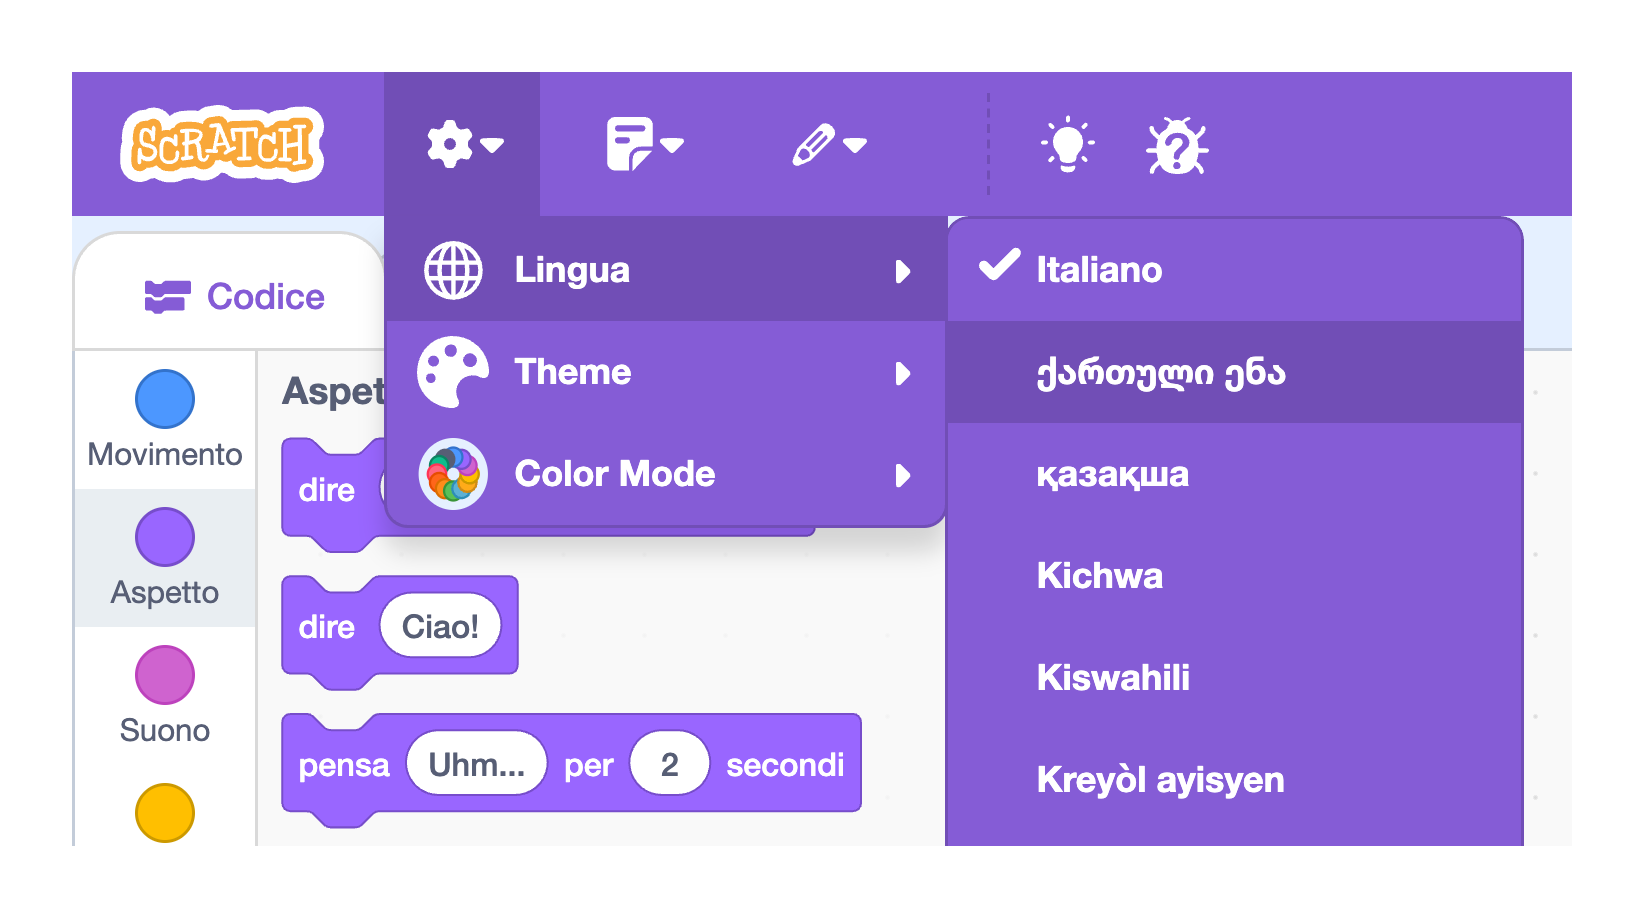
\includegraphics[trim=72bp 72bp 72bp 72bp,clip,width=0.65\linewidth]{img/scratch-lingua.png}\label{credito:scratch-lingua-1}
\end{center}
\newpage

Per modificare la lingua è sufficiente aprire il menu \textbf{Impostazioni} ➜ \textbf{Lingua} e selezionare l'opzione desiderata. L'interfaccia si aggiornerà immediatamente, rendendo i blocchi e i comandi più accessibili e consentendo ai bambini di partecipare con maggiore sicurezza alle attività di programmazione.

Dal menu Impostazioni è possibile scegliere anche colori ad elevato contrasto per facilitare la distinzione dei blocchi.

\end{consiglio}

Ecco come appare la finestra di Scratch dopo averla aperta sul proprio pc.

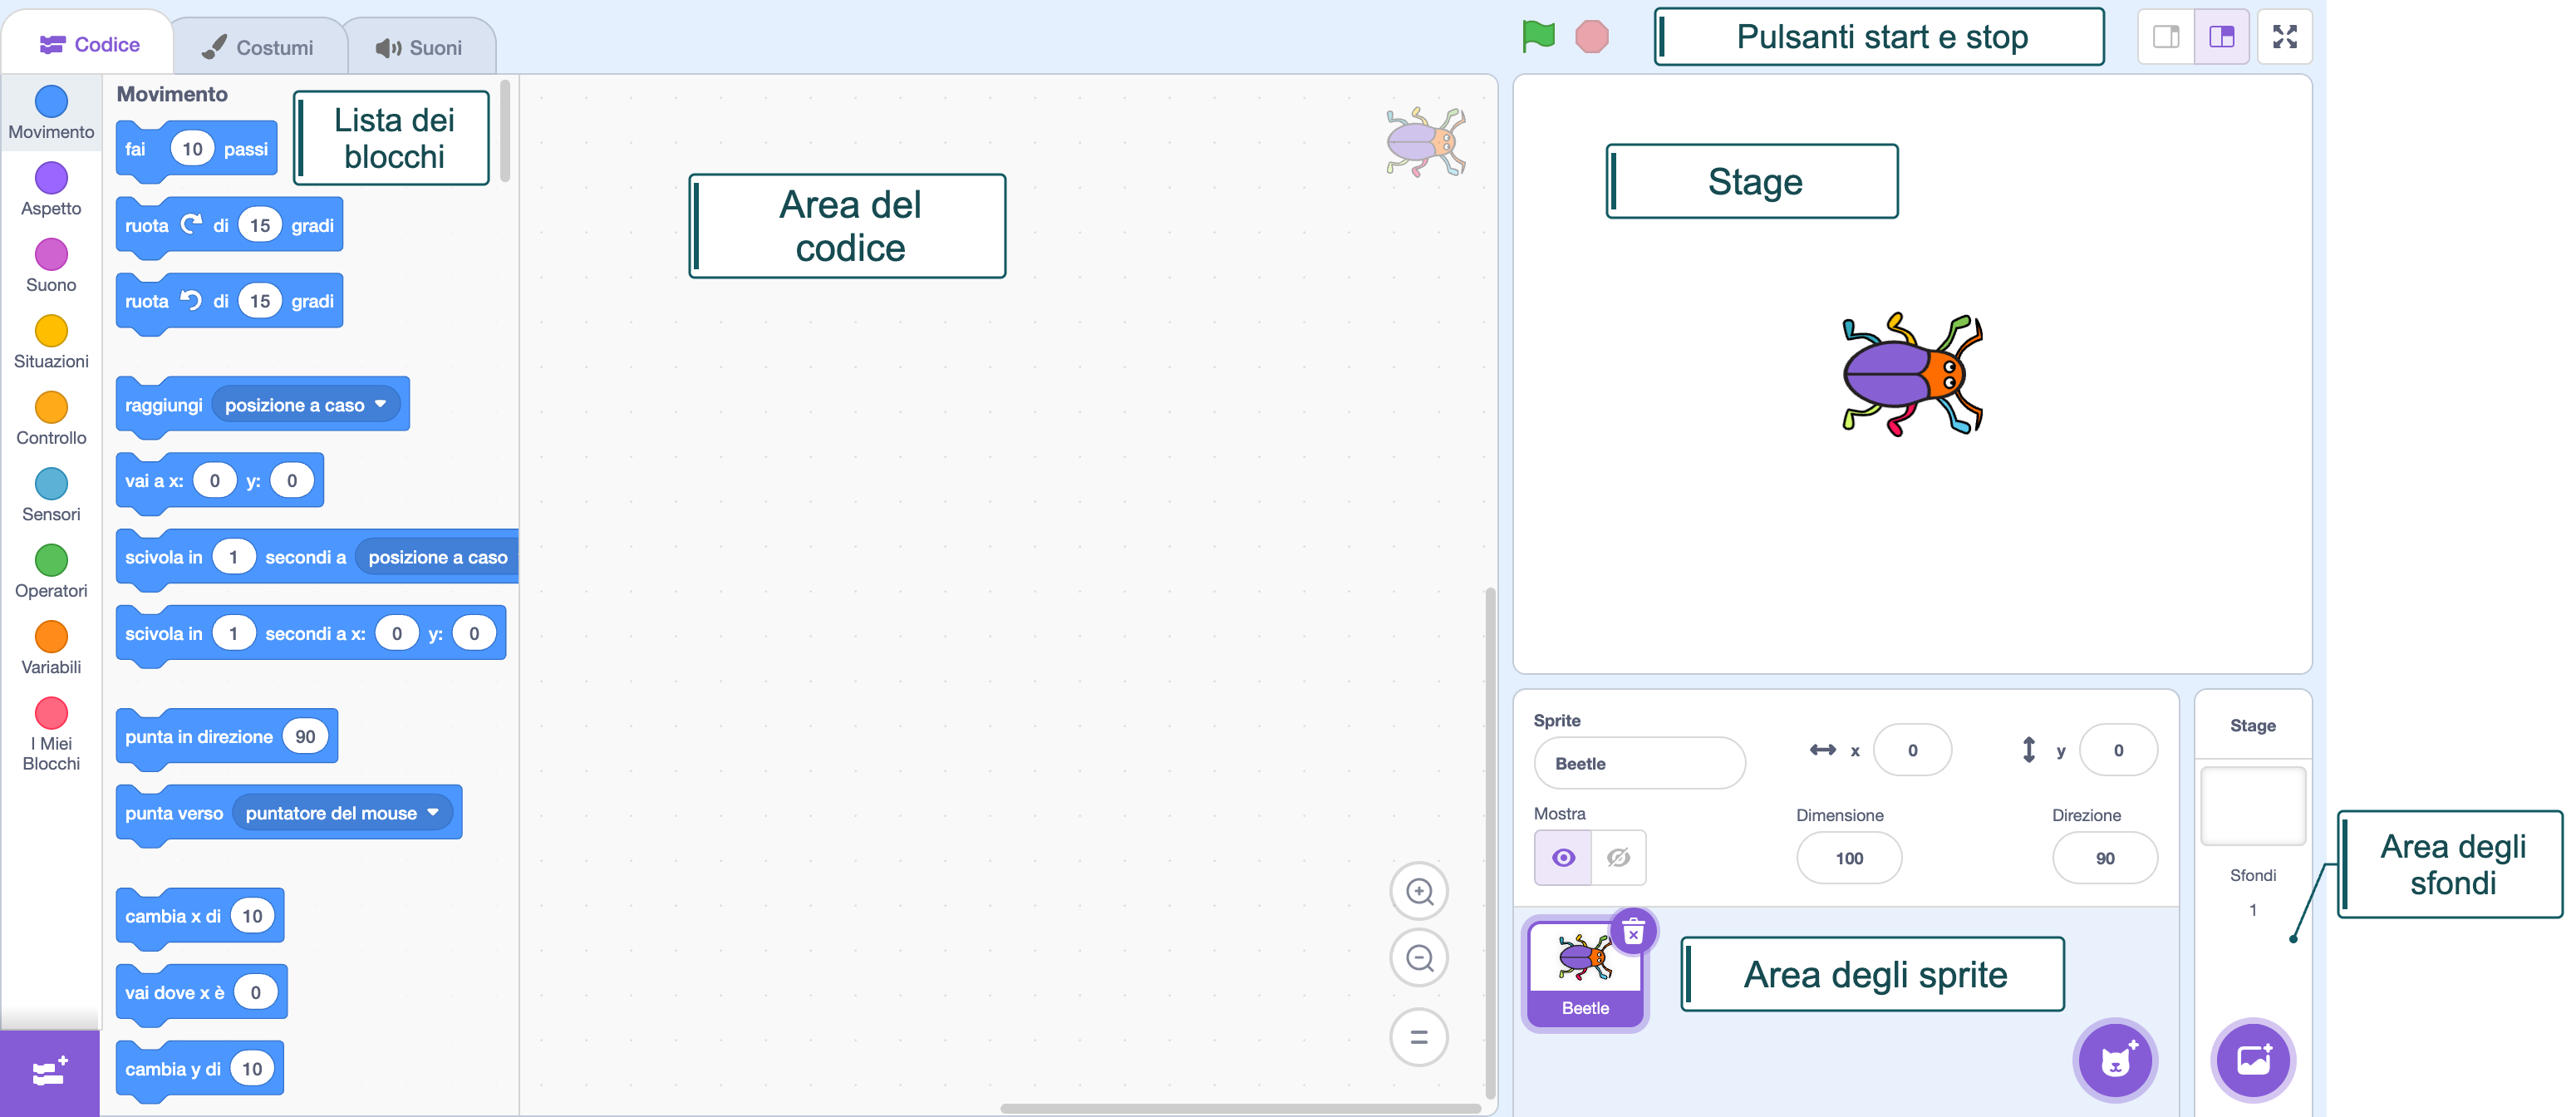
\includegraphics[width=\linewidth]{img/scratch-interfaccia.png}\label{credito:scratch-interfaccia-1}

L'interfaccia di Scratch è organizzata in aree ben distinte, pensate per aiutare gli alunni e le alunne a costruire i propri progetti in modo semplice e intuitivo. Nell'immagine sono visibili le principali aree dell'interfaccia: Lista dei blocchi, Area del codice, stage, Aree degli sprite e degli sfondi. Comprendere la funzione di ciascuna parte è fondamentale per accompagnare alunni e alunne nei primi passi della programmazione.

\begin{itemize}
\item
  \textbf{Lista dei blocchi} (a sinistra)\textbf{:} l'elenco dei blocchi disponibili, come quello presente nei Manuali delle istruzioni, divisi per categorie e riconoscibili grazie al codice colore.
\item
  \textbf{Area del codice} (al centro): lo spazio per costruire i programmi, trascinando nell'area i blocchi presi dalla lista dei blocchi e incastrandoli tra loro. Ogni personaggio (chiamato \textbf{sprite}) avrà il \textbf{proprio codice}: quando si seleziona uno sprite, l'Area del codice mostra quello relativo a quel personaggio.
\item
  \textbf{Stage} (in alto a destra): la scena in cui si svolge l'animazione o il gioco che si sta costruendo. Nello stage si vedono i personaggi in movimento, gli sfondi scelti e gli effetti delle azioni che hanno programmato. In alto compaiono anche i \textbf{pulsanti start} (bandierina verde) e \textbf{stop} (cartello stradale rosso).
\item
  \textbf{Area degli sprite} (in basso a destra): qui sono mostrati gli sprite presenti nel progetto, lo sprite selezionato in quel momento (con il contorno azzurro) e le proprietà dello sprite selezionato (posizione con coordinate x e y, direzione, visibilità, dimensione). Da qui è possibile aggiungere nuovi sprite, cancellarli e duplicarli.
\item
  \textbf{Area degli sfondi} (accanto all'Area degli sprite), dove è possibile cambiare o aggiungere sfondi allo stage.
\end{itemize}


In sintesi, l'immagine mostra \textbf{dove si trovano i blocchi} (colonna sinistra), \textbf{dove si costruisce il programma} (zona centrale), \textbf{dove si vede il risultato} (lo stage in alto a destra), \textbf{dove si gestiscono i personaggi} e \textbf{gli sfondi} (in basso a destra).

\section{Attività 2: diventa un regista con Scratch!}

\ruoliattivita{\ruoloProgrammatore}


In questa attività viene chiesto a bambini e bambine di diventare registi creando un'animazione con un dialogo, in cui il nostro personaggio potrà parlare tramite fumetti.

Prima di lavorare sul codice, vediamo come inserire uno sprite e uno sfondo. Per creare un \textbf{nuovo sprite} bisogna premere sull'icona con la faccia del gatto e scegliere uno dei modi possibili (dall'alto verso il basso):

\noindent
\begin{minipage}[c]{0.81\linewidth}
\begin{itemize}
\item
  caricare un file;
\item
  farlo scegliere a Scratch in maniera casuale;
\item
  disegnarlo;
\item
  sceglierlo dalla libreria di Scratch.
\end{itemize}
\end{minipage}\hfill
\begin{minipage}[c]{0.15\linewidth}
\centering

\includegraphics[height=3.8cm]{img/scratch-menu-sprite.png}\label{credito:scratch-menu-sprite-1}
\end{minipage}
\par

Per creare un \textbf{nuovo sfondo} bisogna premere sull'icona in basso a destra dello schermo e scegliere uno dei modi possibili (dall'alto verso il basso):

\noindent
\begin{minipage}[c]{0.81\linewidth}
\begin{itemize}
\item
  caricare un file;
\item
  farlo scegliere a Scratch in maniera casuale;
\item
  disegnarlo;
\item
  sceglierlo dalla libreria di Scratch.
\end{itemize}
\end{minipage}\hfill
\begin{minipage}[c]{0.15\linewidth}
\centering

\includegraphics[height=3.8cm]{img/scratch-menu-sfondo.png}\label{credito:scratch-menu-sfondo-1}
\end{minipage}
\par


\subsection{E ora, crea il codice!}


Un programma è composto da una serie di blocchi colorati (tra quelli disponibili nella lista dei blocchi, a sinistra dello schermo) agganciati sequenzialmente uno sotto l'altro.

In Scratch ogni blocco ha un colore che identifica la categoria di comandi a cui appartiene: questo aiuta alunni e alunne a riconoscerne rapidamente la funzione e, con il tempo, a intuire che cosa fa un blocco ancora prima di usarlo; puoi decidere se presentarli passo passo oppure lasciare che li esplorino liberamente, sfruttando proprio il colore come guida pratica.

\begin{itemize}
\item
  \textbf{Movimento} (blu): istruzioni che fanno muovere lo sprite sulla scena.
\item
  \textbf{Aspetto} (viola): istruzioni per far ``parlare'' e ``pensare'' uno sprite (con il meccanismo dei fumetti, quindi visualizzando del testo) e per cambiare il suo aspetto.
\item
  \textbf{Suono} (rosa): istruzioni per riprodurre dei suoni.
\item
  \textbf{Situazioni} (giallo): istruzioni per avviare una sequenza di istruzioni come reazione ad un evento, come il click sulla bandierina verde o la pressione di un tasto.
\item
  \textbf{Controllo} (arancione): istruzioni che gestiscono il flusso del programma, permettendo di ripetere azioni, prendere decisioni, attendere, fermare l'esecuzione.
\item
  \textbf{Sensori} (azzurro): istruzioni che permettono allo sprite di ottenere informazioni dall'ambiente (per esempio posizione del mouse, tasti premuti o contatto con altri oggetti) e usarle per guidare il comportamento del programma.
\item
  \textbf{Operatori} (verde): istruzioni per eseguire operazioni aritmetiche, operazioni logiche (cioè verifiche di tipo vero/falso utili a decidere come far agire lo sprite) e per lavorare con i testi.
\item
  \textbf{Variabili e liste} (arancione chiaro): istruzioni per memorizzare informazioni e riutilizzarle nel programma, ad esempio per salvare il punteggio di un gioco.
\end{itemize}

\begin{center}
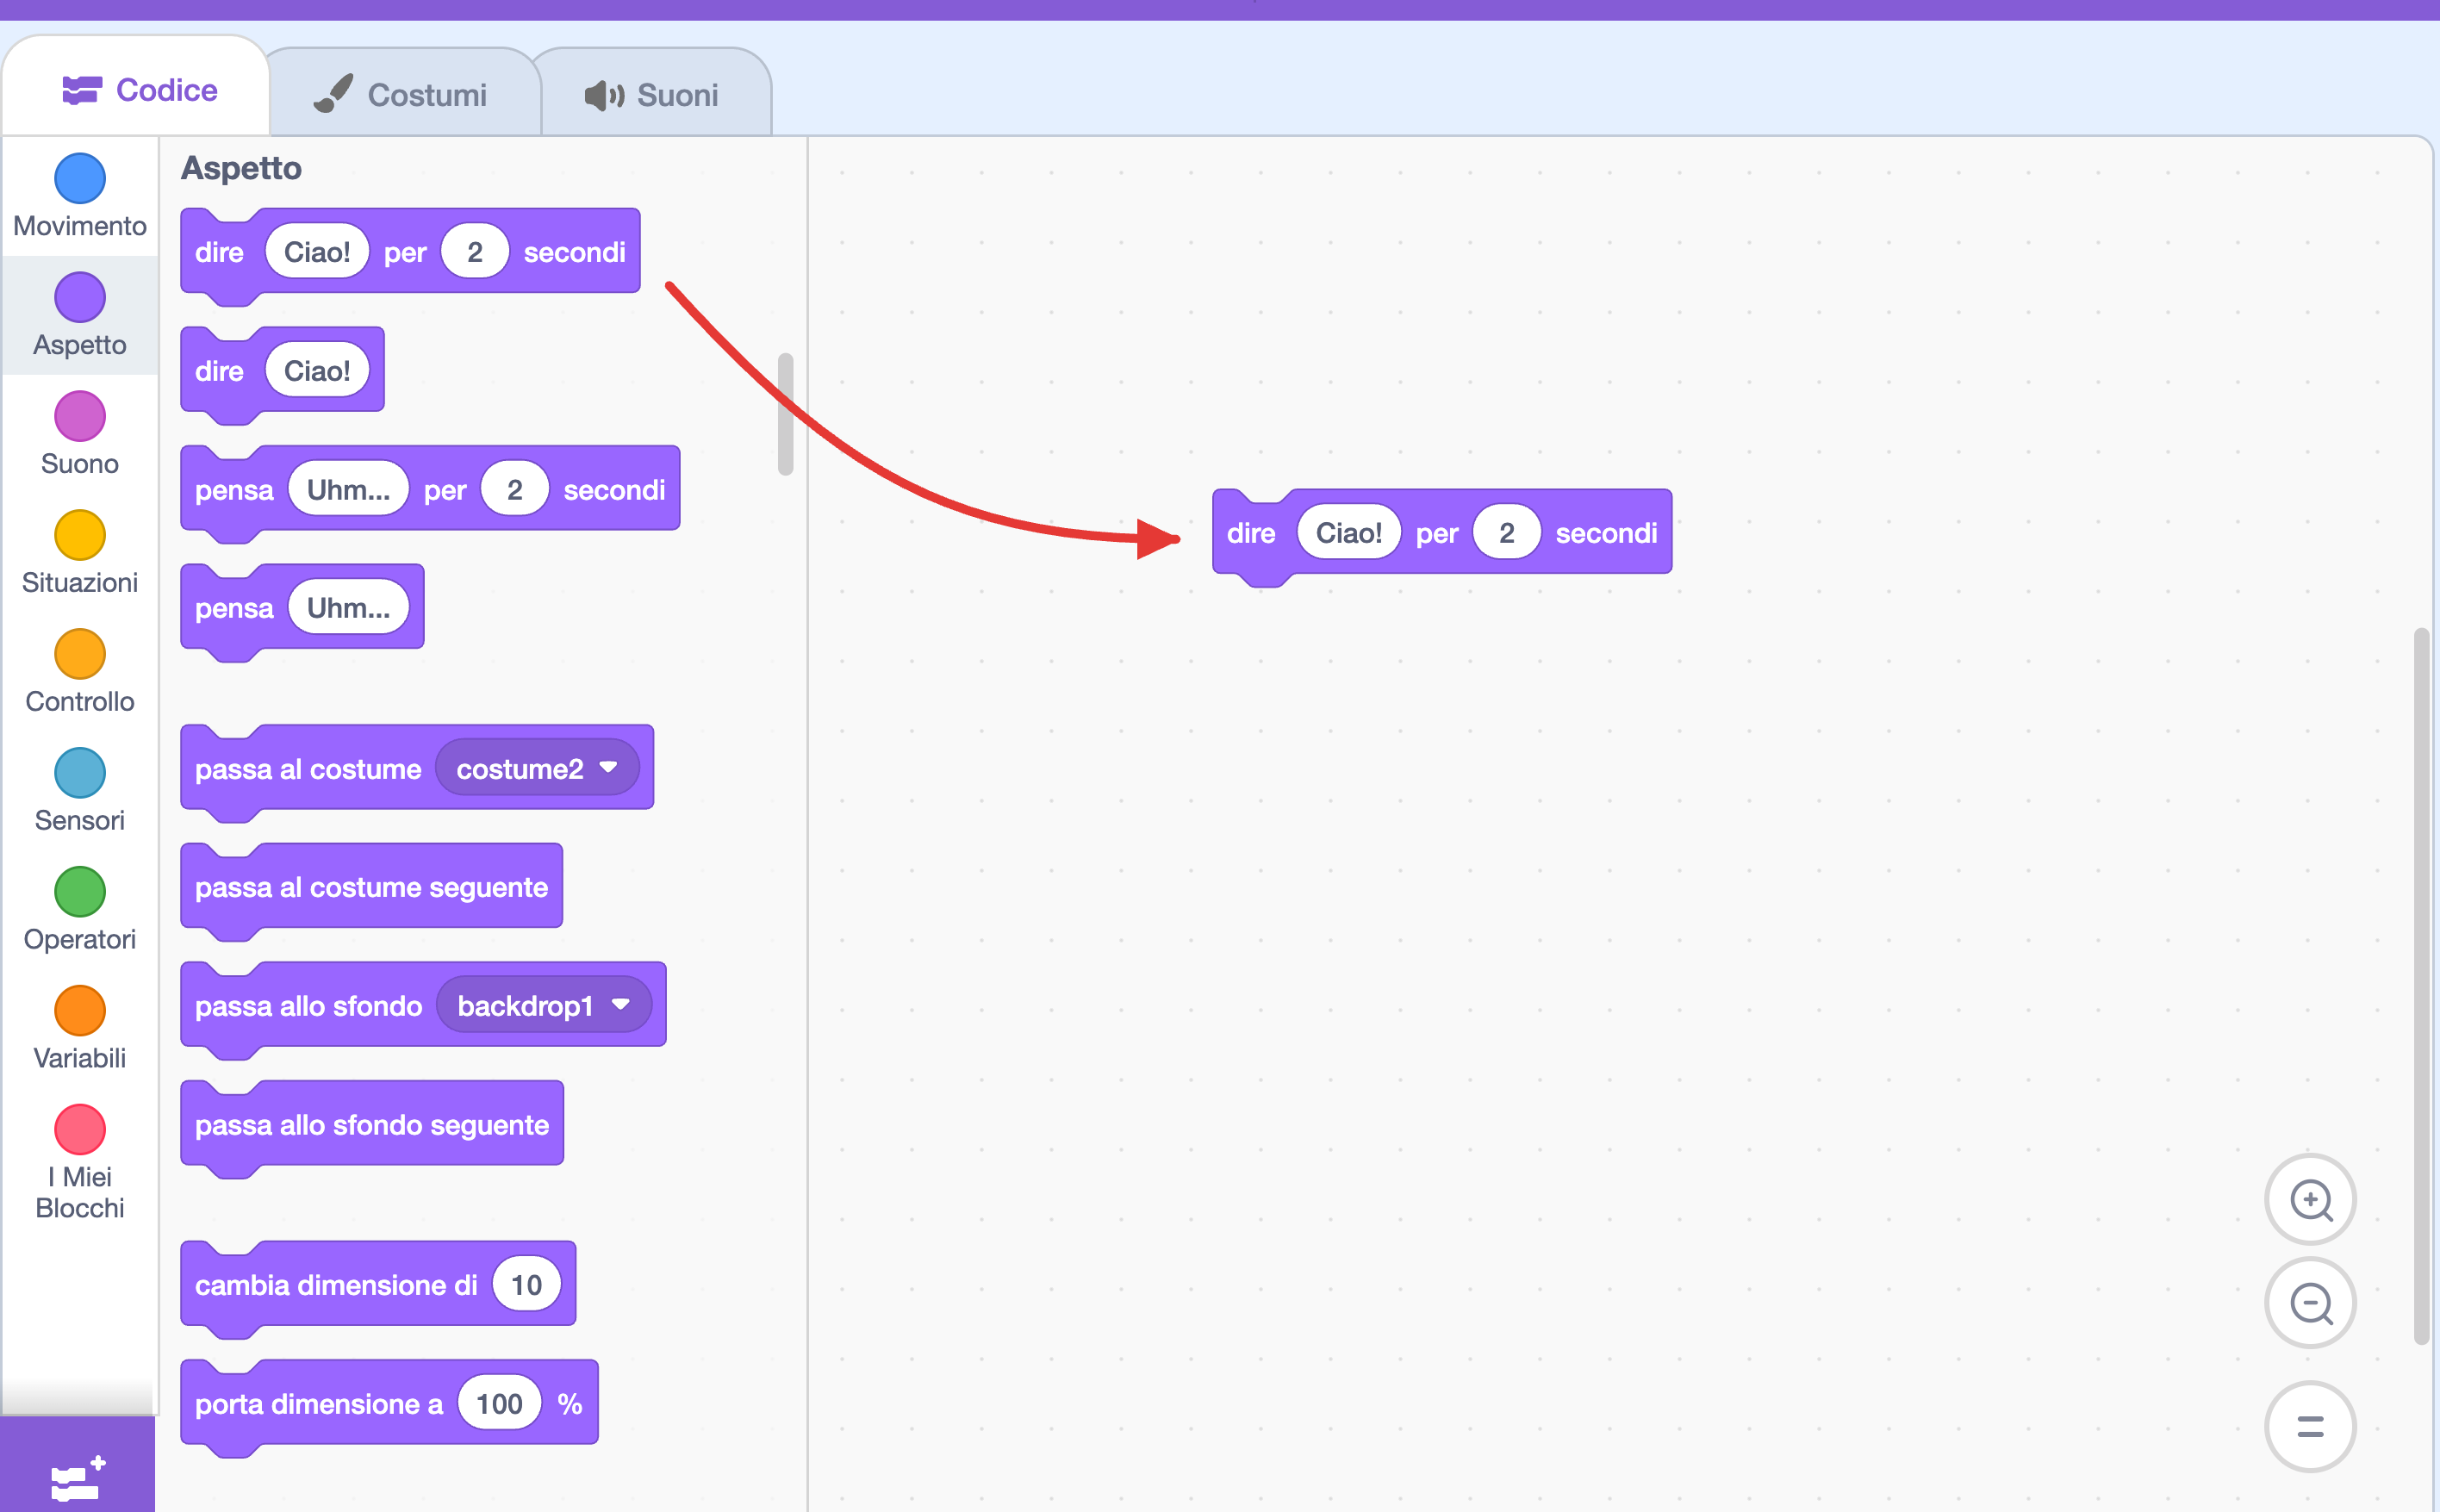
\includegraphics[width=\linewidth]{img/scratch-trascinamento.png}\label{credito:scratch-trascinamento-1}
\end{center}

In questa guida, ci concentreremo su Movimento, Suono, Aspetto, Situazioni e Controllo, mentre Sensori, Operatori e Variabili e liste verranno descritti nel secondo volume.

Dall'Area dei blocchi si possono trascinare i blocchi nell'Area del codice per costruire un programma. I blocchi si agganciano tra loro in sequenza, come pezzi di un puzzle, e ogni sprite esegue le istruzioni dall'alto verso il basso. È possibile spostare, aggiungere o togliere blocchi in qualsiasi momento, modificando così il comportamento dello sprite.

\newpage
Perché Scratch possa eseguire correttamente le istruzioni, i blocchi devono essere incastrati tra loro. Nella figura seguente, il blocco a sinistra è agganciato correttamente, mentre gli altri due non lo sono: se i blocchi restano separati, verranno ignorati da Scratch.

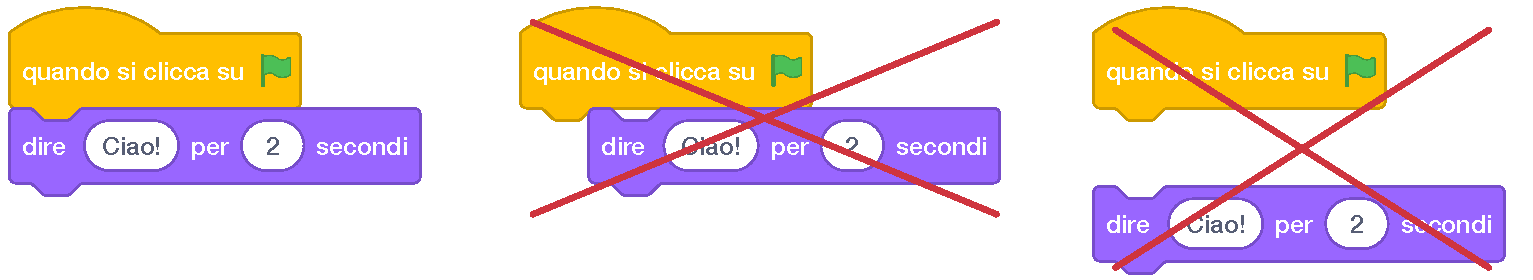
\includegraphics[width=0.9\linewidth]{img/scratchblocks-cap08/pdf/scratch-agganciati.pdf}\label{credito:scratch-agganciati-1}

\Needspace{12\baselineskip}
Il programma, in questo caso, è composto da due istruzioni:

\begin{itemize}
\item
  
\includegraphics[width=99.5bp]{img/scratchblocks-cap08/pdf/scratch-bandiera.pdf}\label{credito:scratch-bandiera-1} (\textbf{Situazioni}): indica che il programma inizierà quando l'utente cliccherà sul pulsante start (la bandiera verde che si trova sopra allo stage).
\item
  
\includegraphics[width=137.5bp]{img/scratchblocks-cap08/pdf/testo-dire-ciao.pdf}\label{credito:testo-dire-ciao-1} (\textbf{Aspetto}): fa comparire sullo sprite un fumetto con la scritta ``Ciao!'' per 2 secondi. Il numero di secondi da inserire dipende dalla lunghezza del testo e dal tempo necessario a chi guarda per leggerlo con calma: per frasi più lunghe può essere utile aumentare l'attesa.
\end{itemize}


In Scratch alcuni blocchi contengono parti già definite e parti ``in bianco'' che possono essere modificate. Queste parti modificabili si chiamano \textbf{parametri}: basta cliccarci sopra per cambiare il valore. Ad esempio, nel blocco 
\includegraphics[width=137.5bp]{img/scratchblocks-cap08/pdf/testo-dire-ciao.pdf}\label{credito:testo-dire-ciao-2} è possibile scrivere il testo che comparirà nel fumetto e decidere per quanti secondi mostrarlo.

Fai scegliere a ciascuno un personaggio e due o tre frasi da fargli pronunciare con i blocchi ``dire''.

\newpage
\section{Attività 3: dialogo tra due personaggi}

\ruoliattivita{\ruoloProgrammatore}

\subsection{Sincronizzazione}


Quando ci sono più personaggi, ciascuno può avere il proprio blocco 
\includegraphics[width=99.5bp]{img/scratchblocks-cap08/pdf/scratch-bandiera.pdf}\label{credito:scratch-bandiera-2}.

In questo caso, tutti gli sprite inizieranno ad eseguire il loro codice nello stesso momento.

Se, ad esempio, abbiamo un blocco 
\includegraphics[width=127.5bp]{img/scratchblocks-cap08/pdf/scratch-dire-ciao.pdf}\label{credito:scratch-dire-ciao-1} in ognuno di loro, tutti mostreranno il fumetto contemporaneamente. Se però vogliamo che parlino uno alla volta, o che uno sprite inizi a muoversi solo dopo che un altro ha finito, dobbiamo \textbf{sincronizzare} le loro azioni, cioè decidere l'ordine e i momenti in cui ogni sprite deve attivarsi.

Prendiamo come esempio un dialogo tra un ippopotamo e un ragnetto (mostrato per intero nella figura).

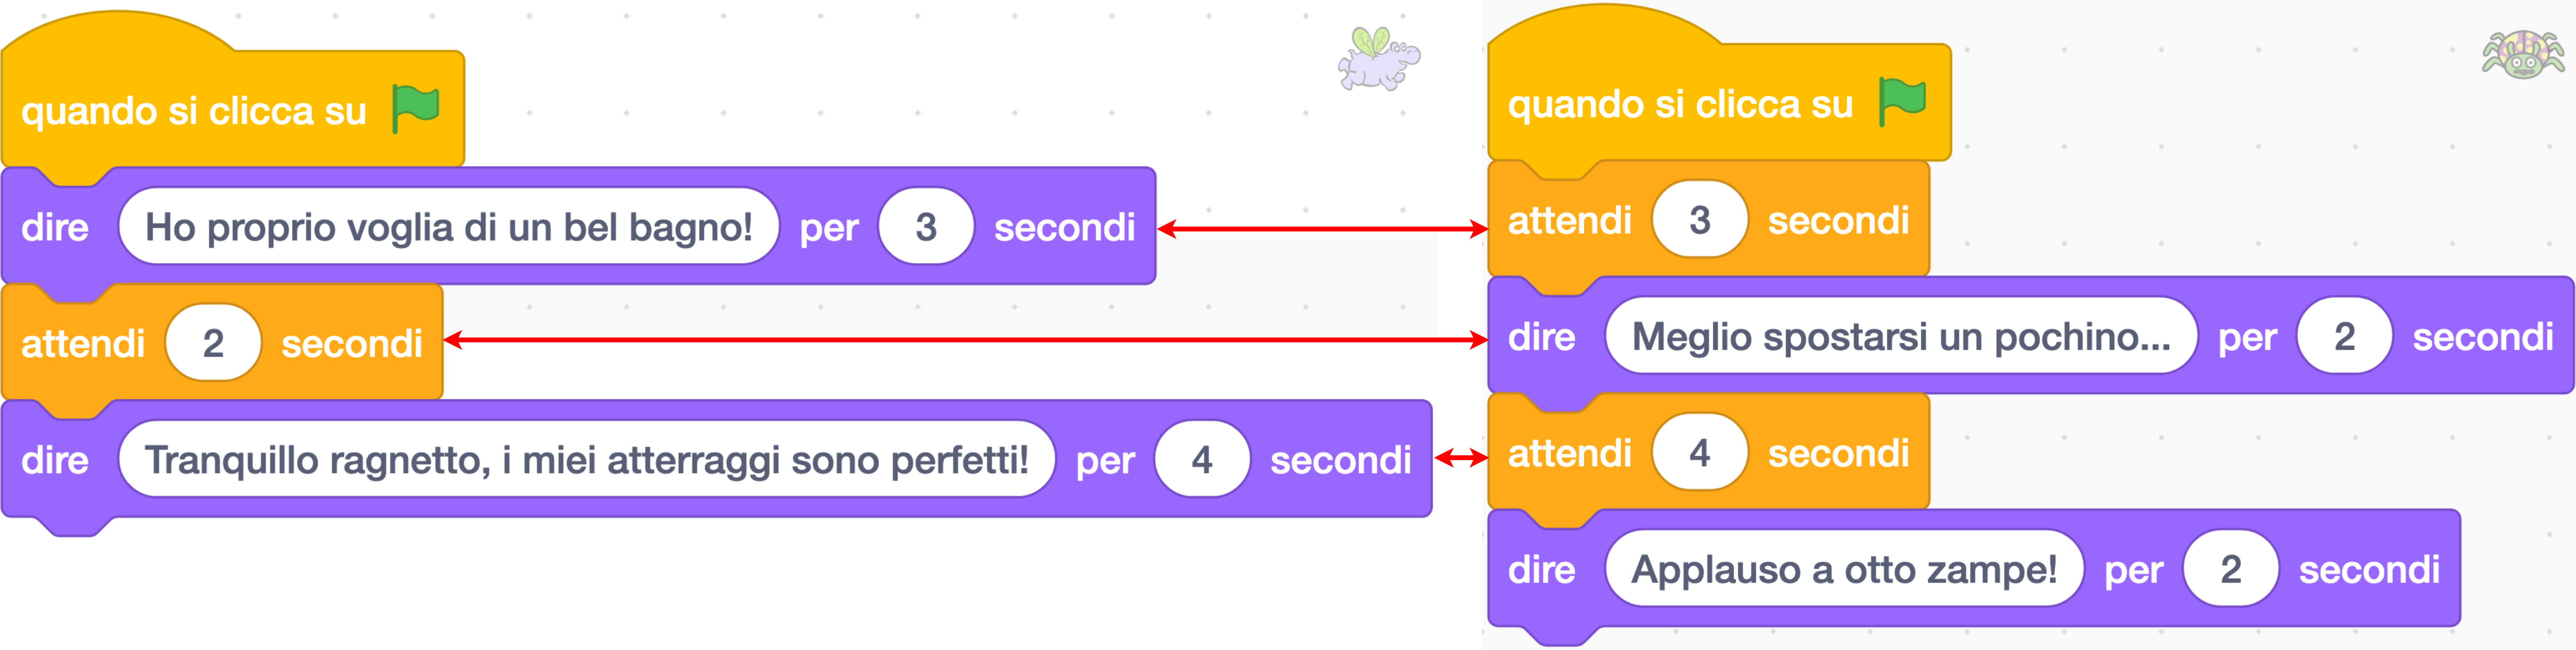
\includegraphics[width=\linewidth]{img/scratch-dialogo.png}\label{credito:scratch-dialogo-1}

L'ippopotamo pronuncia la prima battuta e solo dopo alcuni secondi il ragnetto\footnote{Lo sprite scelto è Ladybug2, che, stando al nome, è una coccinella. Continueremo a chiamarlo ``ragnetto'' per maggiore suggestività. Al lettore pignolo facciamo notare che l'ippopotamo ha due ali da insetto \emoji{wink}} risponde. Per ottenere questo comportamento ordinato non basta mettere i blocchi in sequenza: bisogna dire allo sprite \textbf{quando} deve iniziare la sua azione.


Utilizziamo il blocco 
\includegraphics[width=97bp]{img/scratchblocks-cap08/pdf/scratch-attendi.pdf}\label{credito:scratch-attendi-1} (\textbf{Controllo}), qui a fianco, che permette allo sprite di fare una pausa prima di passare alle istruzioni successive. In questo esempio, il ragnetto aspetta 3 secondi, cioè il tempo che serve per far finire la frase all'ippopotamo: come si vede nella figura, i blocchi attendi permettono ai personaggi di parlare uno dopo l'altro, senza sovrapporsi.


Prima di programmare può essere utile creare un piccolo storyboard: una sequenza di vignette o appunti che raccontano, passo dopo passo, cosa succederà nella storia o nell'animazione. Questo passaggio permette a ciascuno di pianificare con chiarezza le scene, decidere chi parla, chi si muove e quando, e trasformare l'idea in un progetto ordinato. Lavorare con uno storyboard evita confusione in fase di programmazione e aiuta a mantenere una visione d'insieme del progetto.

\begin{center}
\setlength{\tabcolsep}{4pt}
\setlength{\arrayrulewidth}{0.5pt}
\renewcommand{\arraystretch}{1.45}
\begin{tabular}{|*{2}{>{\centering\arraybackslash}m{\dimexpr0.4\linewidth-2\tabcolsep-1.25\arrayrulewidth\relax}|>{\centering\arraybackslash}m{\dimexpr0.1\linewidth-2\tabcolsep-1.25\arrayrulewidth\relax}|}}
\arrayrulecolor{black!40}
\hline
\rowcolor{black!12}
\multicolumn{2}{|>{\centering\arraybackslash}m{\dimexpr0.5\linewidth-2\tabcolsep-1.5\arrayrulewidth\relax}|}{\textbf{Personaggio: Lupo}} &
\multicolumn{2}{>{\centering\arraybackslash}m{\dimexpr0.5\linewidth-2\tabcolsep-1.5\arrayrulewidth\relax}|}{\textbf{Personaggio: Cappuccetto Rosso}} \\
\hline
Ciao bella bambina! & 3 & \multirow[t]{2}{*}{ATTENDI} & \multirow[t]{2}{*}{5} \\
\cline{1-2}
Come ti chiami? & 2 & & \\
\hline
ATTENDI & 4 & Mi chiamo Cappuccetto Rosso! & 4 \\
\hline
Ma che bel nome! & 2 & ATTENDI & 2 \\
\hline
\end{tabular}
\end{center}



\subsection{Ripetizione}\label{ripetizione}

\noindent
\begin{minipage}[t]{0.28\linewidth}
\vspace{0pt}
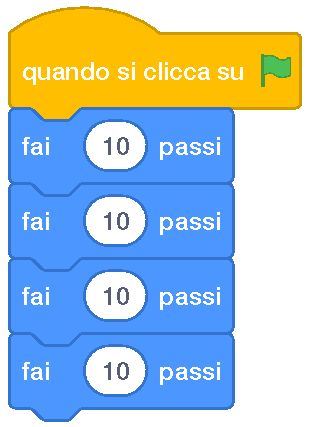
\includegraphics[width=99.5bp]{img/scratchblocks-cap08/pdf/scratch-programma-lungo.pdf}\label{credito:scratch-programma-lungo-1}
\end{minipage}\hfill
\begin{minipage}[t]{0.68\linewidth}
\vspace{0pt}
Supponiamo che il ragnetto non si fidi delle doti dell'ippopotamo e voglia spostarsi sullo schermo. Per farlo potrebbe usare più volte il blocco 
\includegraphics[width=78bp]{img/scratchblocks-cap08/pdf/scratch-fai10.pdf}\label{credito:scratch-fai10-1}, come nel programma qui a fianco, ma il programma diventerebbe lungo, difficile da leggere e da modificare.
\end{minipage}

\noindent
\begin{minipage}[t]{0.28\linewidth}
\vspace{0pt}

\includegraphics[width=86bp]{img/scratchblocks-cap08/pdf/scratch-ripeti-vuoto.pdf}\label{credito:scratch-ripeti-vuoto-1}
\end{minipage}\hfill
\begin{minipage}[t]{0.68\linewidth}
\vspace{0pt}
Per rendere il codice più semplice possiamo usare il blocco \textbf{ripeti \ldots{} volte} (\textbf{Controllo}). Questo blocco ha la forma di una ``C'' aperta: la sequenza delle istruzioni inserite al suo interno verrà ripetuta per il numero di volte indicato. Le istruzioni che si trovano fuori dalla ``C'' non verranno ripetute.
\end{minipage}

\Needspace{14\baselineskip}
\begin{consiglio}[Maestr* si è buggato... non ripete niente!]

È utile far notare che, soprattutto all'inizio, alunni e alunne incastrano i blocchi nel punto sbagliato: ad esempio, può capitare che il blocco 
\includegraphics[width=78bp]{img/scratchblocks-cap08/pdf/scratch-fai10.pdf}\label{credito:scratch-fai10-2} venga messo prima o dopo la ``C'', pensando che venga comunque ripetuto (nella figura seguente, solo il programma a sinistra ripete il movimento). Mostrare loro l'effetto dell'errore aiuta a comprendere meglio la logica della ripetizione e l'importanza della posizione dei blocchi.

\begin{center}
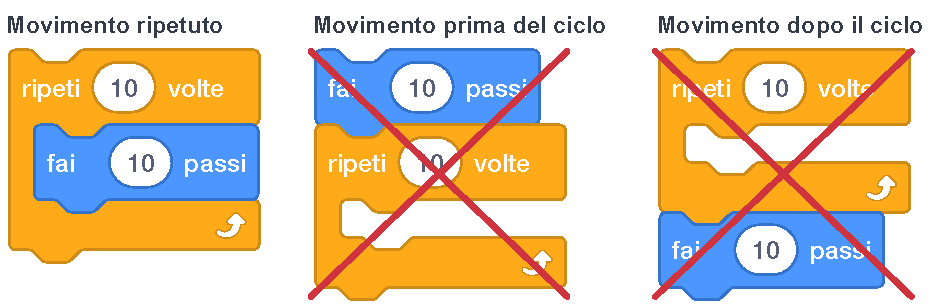
\includegraphics[width=0.92\linewidth]{img/scratchblocks-cap08/pdf/scratch-ripeti-completo.pdf}\label{credito:scratch-ripeti-completo-1}
\end{center}

\end{consiglio}
\newpage
\subsection{Ripetizione infinita}\label{ripetizione-infinita}

Possiamo anche ripetere una sequenza di blocchi all'infinito con il blocco \textbf{per sempre} (\textbf{Controllo}).

\begin{center}

\includegraphics[width=86bp]{img/scratchblocks-cap08/pdf/scratch-persempre-vuoto.pdf}\label{credito:scratch-persempre-vuoto-1}
\end{center}

A differenza del blocco \textbf{ripeti \ldots{} volte}, questo blocco non ha l'incastro sul fondo: significa che il programma continuerà a eseguire all'infinito le istruzioni contenute al suo interno, senza arrivare mai a un blocco successivo. Come nel caso di \textbf{ripeti \ldots{} volte}, verranno ripetuti solo i blocchi inseriti dentro la ``C''.

\noindent
\begin{minipage}[t]{0.34\linewidth}
\vspace{0pt}
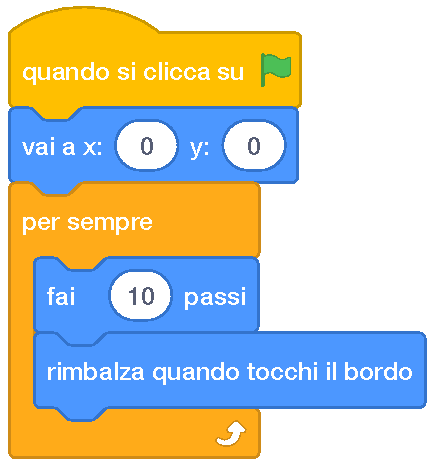
\includegraphics[width=139bp]{img/scratchblocks-cap08/pdf/scratch-persempre1.pdf}\label{credito:scratch-persempre1-1}
\end{minipage}\hfill
\begin{minipage}[t]{0.62\linewidth}
\vspace{0pt}
Nel codice qui a fianco, lo sprite viene prima posizionato al centro dello stage (x: 0, y: 0) e poi, \textbf{per sempre}, fa 10 passi e rimbalza quando tocca il bordo: si muoverà quindi in continuazione avanti e indietro.
\end{minipage}


\Needspace{0.35\textheight}
\begin{consiglio}[Maestr* si è buggato... non si muove!]

\ruoliattivita{\ruoloEsecutore}

\noindent
\begin{minipage}[t]{0.34\linewidth}
\vspace{0pt}
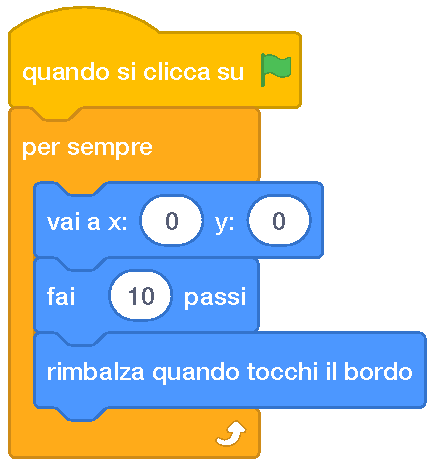
\includegraphics[width=\linewidth]{img/scratchblocks-cap08/pdf/scratch-persempre2.pdf}\label{credito:scratch-persempre2-1}
\end{minipage}\hfill
\begin{minipage}[t]{0.62\linewidth}
\vspace{0pt}
Nel codice qui a fianco, invece, anche il blocco 
\includegraphics[width=98.5bp]{img/scratchblocks-cap08/pdf/scratch-vai-centro.pdf}\label{credito:scratch-vai-centro-1} è inserito dentro la ``C'': in questo caso lo sprite torna al centro dello stage ad ogni ripetizione, fa solo pochi passi e poi ricomincia subito da capo. Il movimento è impercettibile e può sembrare che lo sprite ``non si muova''. In questi casi, può essere utile chiedere al proprio alunno/a di leggere il codice ad alta voce, passo per passo (``cosa succede per primo? e poi? e poi?'') per facilitare il ragionamento di studenti e studentesse sul comportamento dei propri blocchi.
\end{minipage}

\end{consiglio}

\clearpage
\section{Attività 4: movimenti precisi}

\ruoliattivita{\ruoloProgrammatore}

Ogni sprite, oltre al nome, ha diverse proprietà visibili nell'Area degli sprite. In questa sezione è possibile vedere e modificare informazioni come posizione, direzione, dimensione e visibilità, come mostrato nell'immagine.


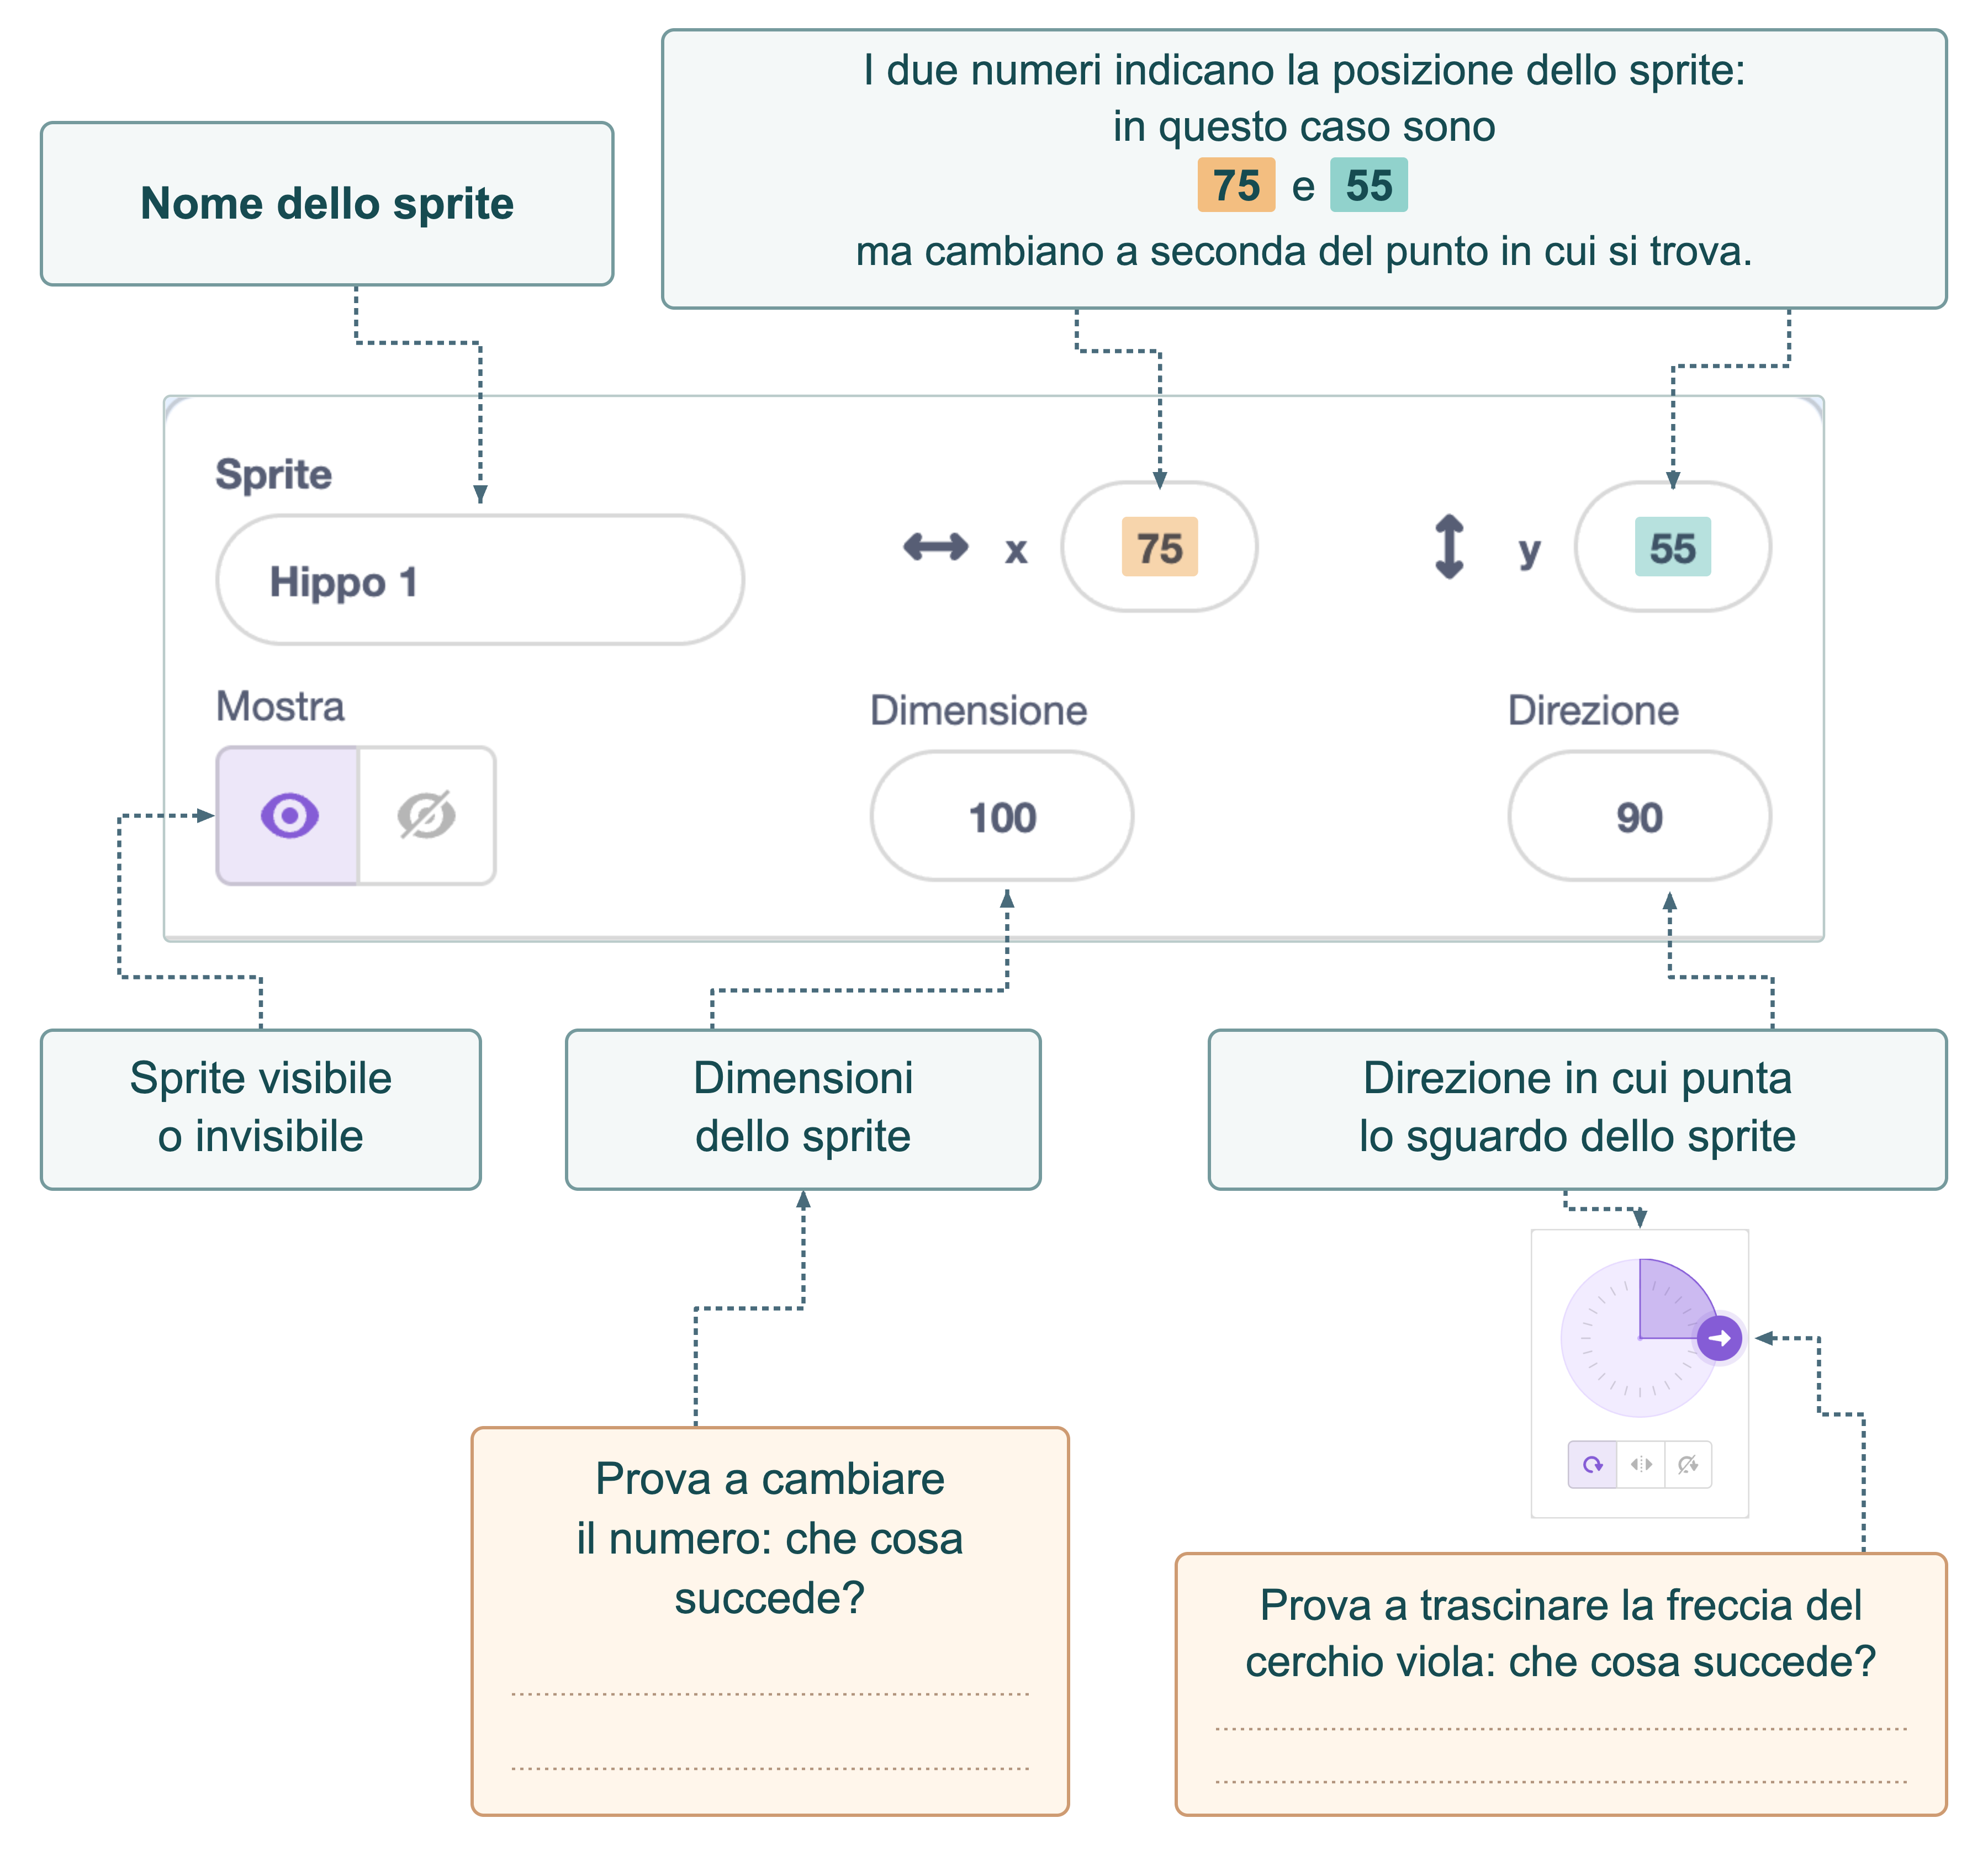
\includegraphics[width=0.9\linewidth]{img/scratch-proprieta-sprite.png}\label{credito:scratch-proprieta-sprite-1}



Incoraggiate alunni e alunne ad esplorare cosa succede cambiando la proprietà \textbf{dimensione} e la proprietà \textbf{direzione} nell'Area degli sprite.


\subsection{La posizione}\label{la-posizione}

\noindent
\begin{minipage}[t]{0.49\linewidth}
\vspace{0pt}
Lo sfondo visibile nell'immagine è uno degli sfondi predefiniti di Scratch (\textbf{Xy-grid}). Mostra allo stesso tempo lo stage e il sistema di coordinate cartesiane che lo struttura. La larghezza misura 480 unità (240 a destra e 240 a sinistra del centro) e l'altezza 360 unità (180 sopra e 180 sotto il centro). Il punto centrale dello stage è indicato dalle coordinate x=0 e y=0: la linea arancione (orizzontale) rappresenta l'asse X, la linea blu (verticale) l'asse Y.
\end{minipage}\hfill
\begin{minipage}[t]{0.48\linewidth}
\vspace{0pt}
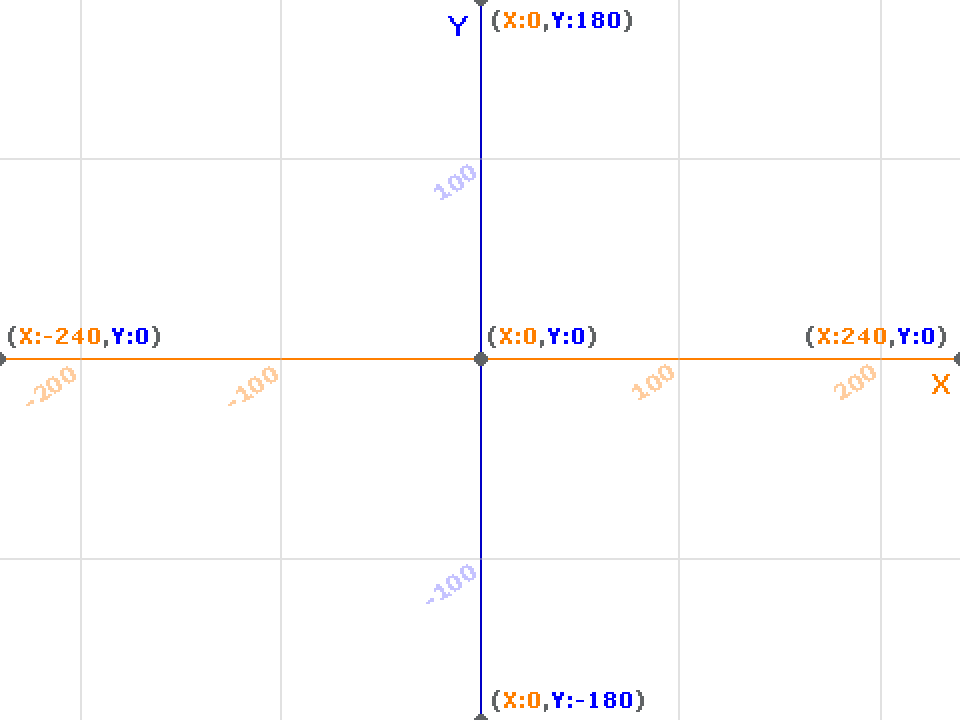
\includegraphics[width=\linewidth]{img/scratch-xy-grid.png}\label{credito:scratch-xy-grid-1}
\end{minipage}
\par

Sebbene in terza primaria sia possibile che piano cartesiano e numeri negativi non siano ancora stati oggetto di insegnamento esplicito, Scratch offre la possibilità di incontrarli in modo naturale e graduale: il semplice fatto di copiare i valori indicati, provare a modificarli e osservare cosa succede ai personaggi può aiutare a orientarsi sullo stage e a prendere confidenza con l'idea di movimento sul piano.

Per questa esplorazione, chiedete di selezionare lo sfondo \textbf{Xy-grid} e lo sprite \textbf{Ball} dalla libreria di Scratch.  Incoraggiate alunni e alunne a esplorare cosa accade cambiando la posizione dello sprite: prima spostandolo con il mouse e osservando come cambiano i valori di x e y, poi scrivendo direttamente dei valori nelle caselle x e y dell'Area degli sprite e osservando dove ``salta'' il personaggio.


\begin{minipage}{\linewidth}
\centering
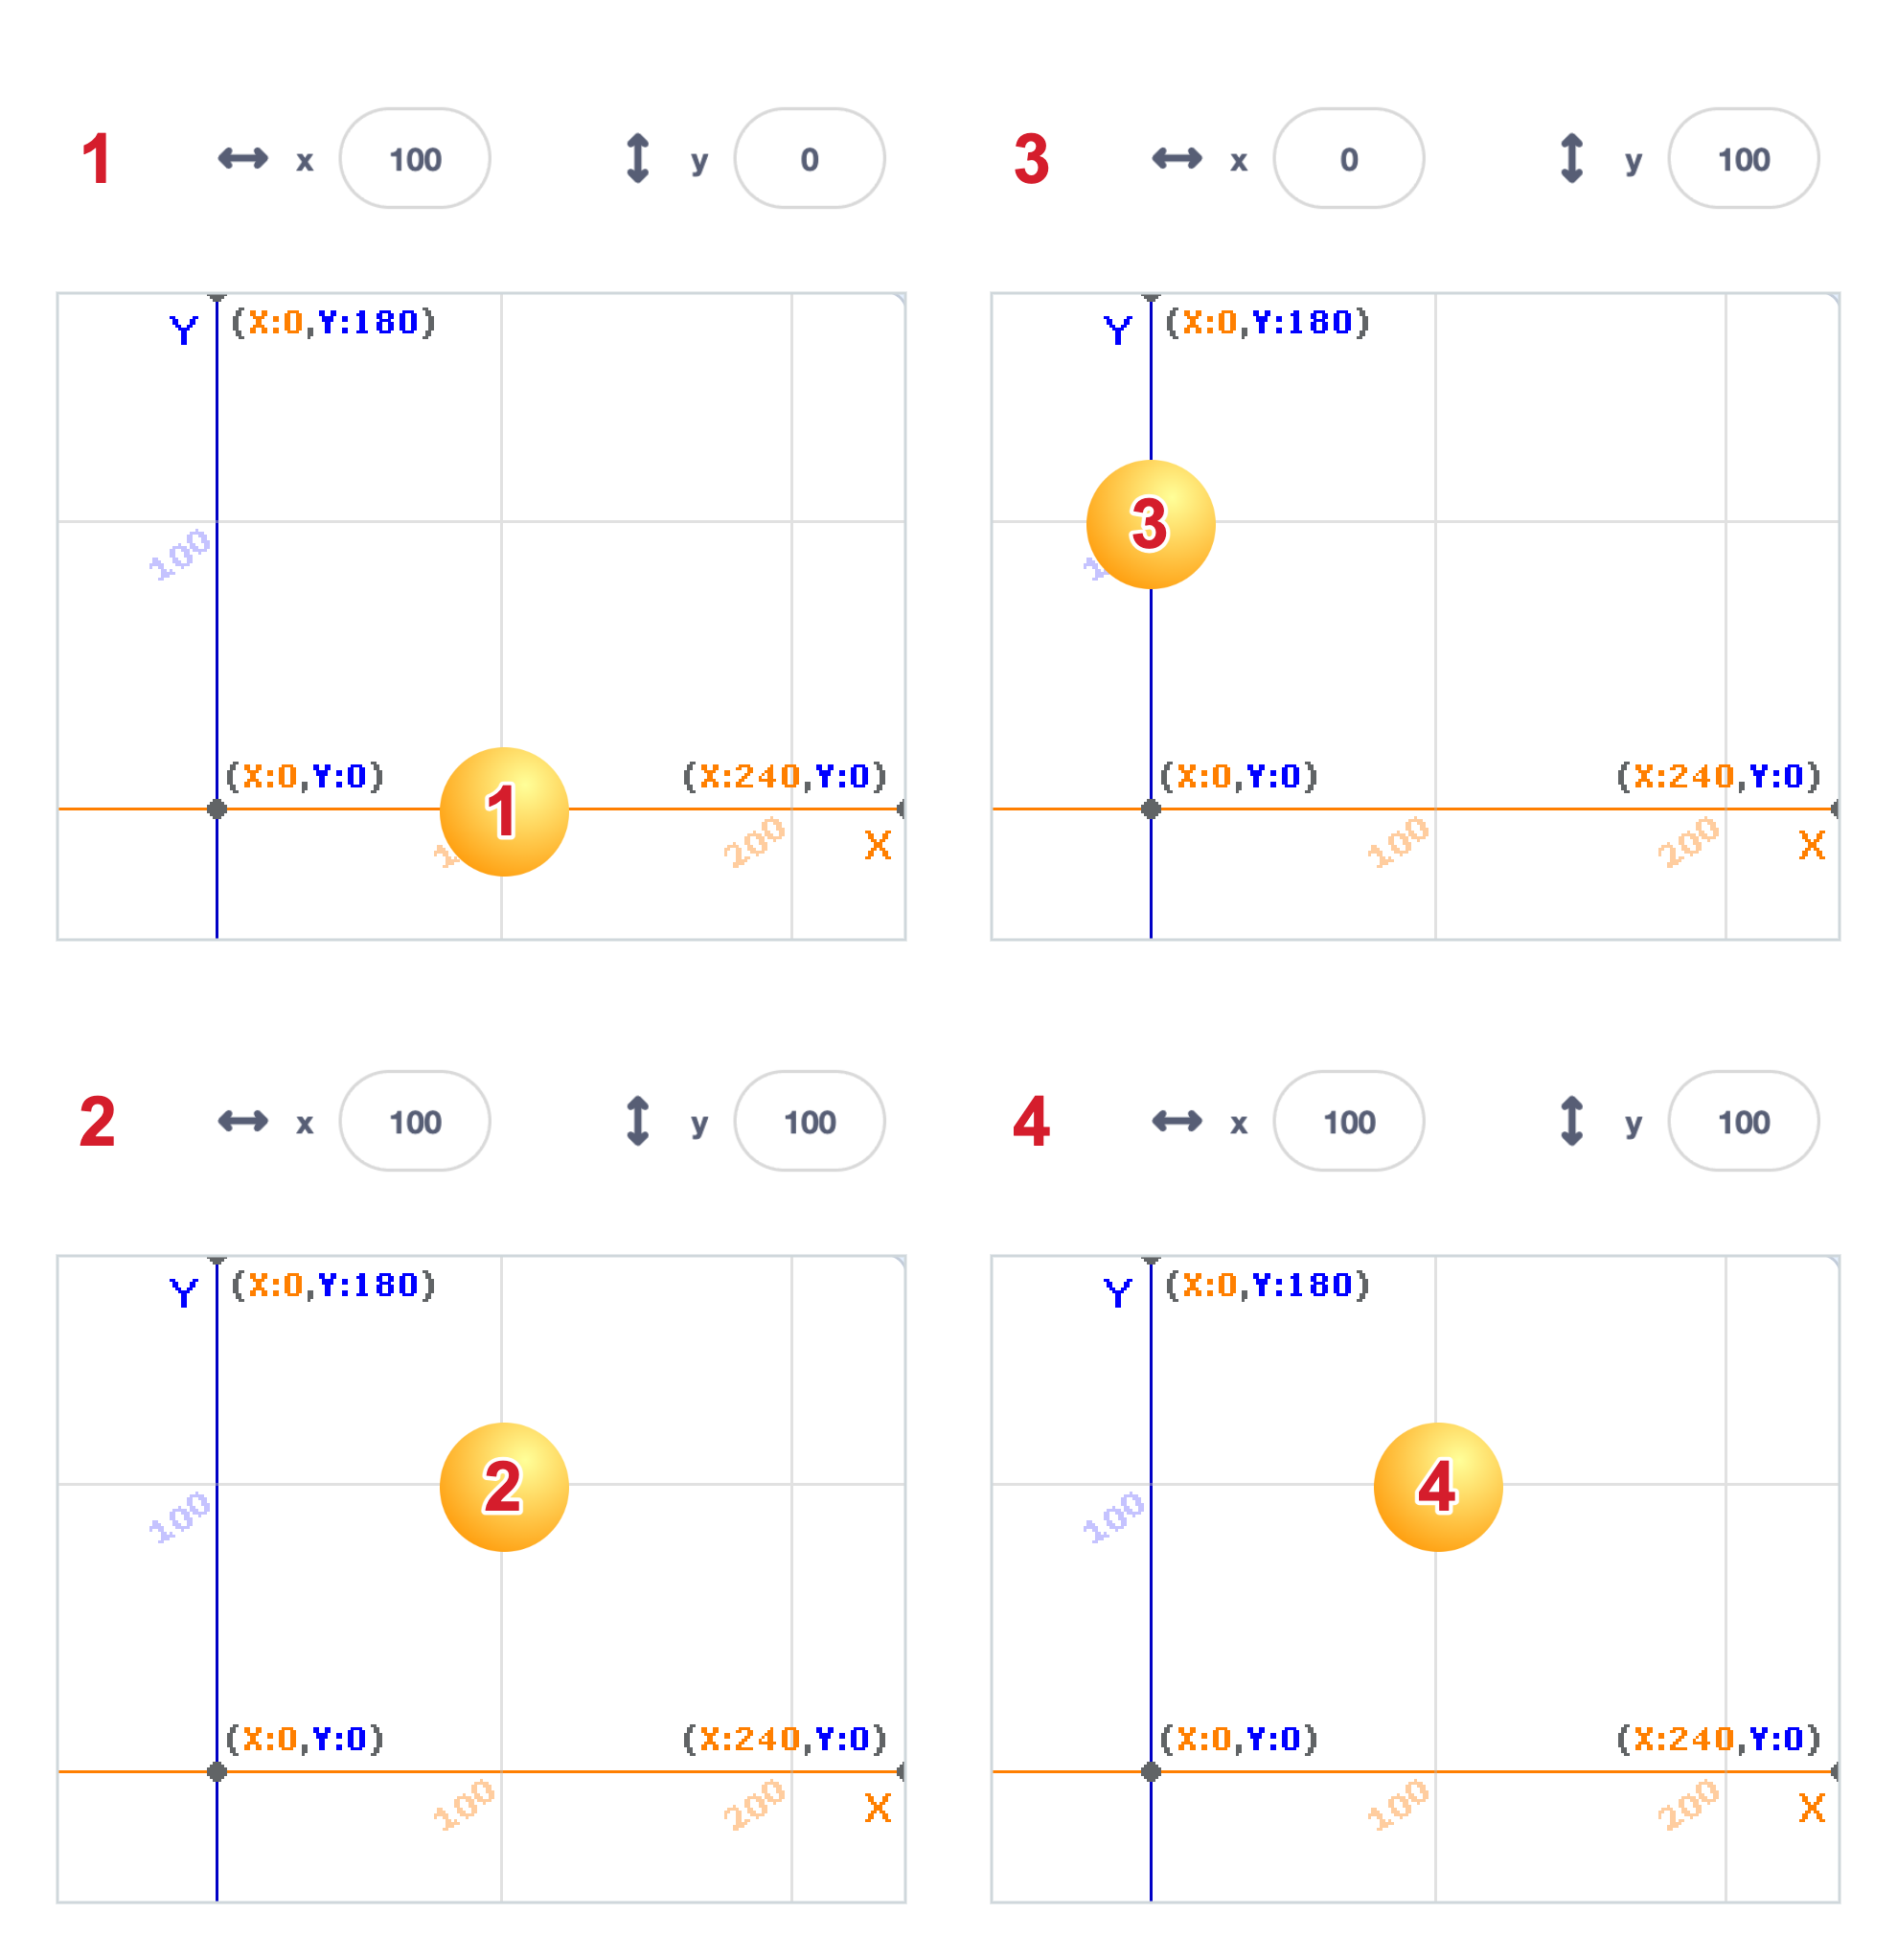
\includegraphics[width=0.8\linewidth]{img/scratch-coordinate.png}\label{credito:scratch-coordinate-1}
\end{minipage}

\section{Attività 5: posizionare un personaggio}

\ruoliattivita{\ruoloProgrammatore}

\subsection{Scegliere una posizione}\label{scegliere-una-posizione}

Il blocco 
\includegraphics[width=98.5bp]{img/scratchblocks-cap08/pdf/scratch-vai-a.pdf}\label{credito:scratch-vai-a-1} (\textbf{Movimento}) permette di posizionare lo sprite in una precisa posizione dello stage. Per trovare le coordinate da inserire, bisogna (1) spostare lo sprite con il mouse nella posizione desiderata, (2) leggere i valori \emph{x} e \emph{y} riportati nell'Area degli sprite e (3) copiarli dentro il blocco. In questo modo il personaggio si sposterà sempre nel punto scelto. Questa procedura aiuta alunni e alunne a scoprire che lo sprite può essere posizionato sia ``a mano'' nell'interfaccia, come se fosse telecomandato, sia usando il blocco di movimento, cioè \textbf{pianificando} in anticipo le azioni. Questo passaggio può aiutare a capire la differenza tra muovere direttamente il personaggio e farlo muovere da solo seguendo le istruzioni del programma.

Proponete di copiare un programma che usa il blocco \textbf{vai a} per fissare la posizione di partenza, ad esempio:
\begin{center}
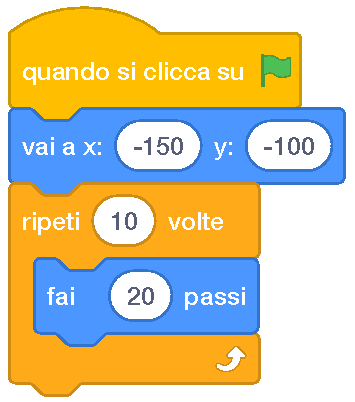
\includegraphics[width=113.5bp]{img/scratchblocks-cap08/pdf/testo-posizione-iniziale.pdf}\label{credito:testo-posizione-iniziale-1}
\end{center}
Incoraggiate bambini e bambine a provare a far partire il personaggio in diversi punti dello schermo, modificando le coordinate di partenza.

\begin{consiglio}[Maestr* si è buggato... perché non comincia come voglio io?]

Al termine dell'esecuzione del programma, può capitare che il personaggio resti in una posizione sullo stage non desiderata. Quando si clicca di nuovo sulla bandierina verde, lo sprite ricomincia a muoversi proprio da lì, rovinando l'effetto voluto.

Questo accade perché ogni personaggio possiede un proprio \textbf{stato}, cioè un insieme di informazioni che Scratch conserva: posizione, direzione, dimensione, visibilità, e così via. In pratica, lo sprite non ``si resetta da solo'': si comporta come un attore un po' distratto, che riparte da dove era rimasto se non gli viene detto con precisione cosa fare.

Per questo è importante inserire all'inizio dello script i blocchi che fissano la posizione di partenza (e, se serve, dimensione e direzione). Un buon trucco in classe è chiedere a ciascuno di leggere a voce alta il proprio codice passo per passo chiedendosi: ``Dove sta il personaggio adesso? Dove gli ho detto di andare? Da dove sta ripartendo?''

Questo aiuta a capire che anche la posizione iniziale fa parte della programmazione.

\end{consiglio}


\subsection{Scegliere una direzione}\label{scegliere-una-direzione}

Nell'Attività precedente abbiamo chiesto agli alunni e alle alunne di esplorare il concetto di direzione. La direzione indica ``dove lo sprite sta guardando'': è come girarsi prima di iniziare a camminare. Come per la posizione, oltre a scegliere la direzione tramite l'interfaccia, è possibile utilizzare il blocco 
\includegraphics[width=104bp]{img/scratchblocks-cap08/pdf/scratch-punta-direzione.pdf}\label{credito:scratch-punta-direzione-1} (\textbf{Movimento}) per pianificare la direzione del movimento.

Questo blocco funziona con gli angoli misurati in gradi e il valore fa riferimento all'ampiezza dell'angolo centrato nell'origine del sistema di riferimento che struttura lo stage e che ha: un lato sul semiasse Y positivo e il secondo lato dato dalla direzione in cui punta lo ``sguardo dello sprite''. Ad esempio, il valore 0 in questo blocco indica che lo sprite deve puntare lo sguardo in una direzione che formi un angolo di ampiezza 0° con il semiasse positivo Y: quindi, lo sprite punterà lo sguardo verso l'alto; inserendo il valore 180 punterà lo sguardo verso il basso, inserendo -90 punterà lo sguardo verso sinistra e con 90 verso destra, come mostrato nella figura~\ref{fig:direzioni-assolute}.

\begin{figure}
  \begin{center}
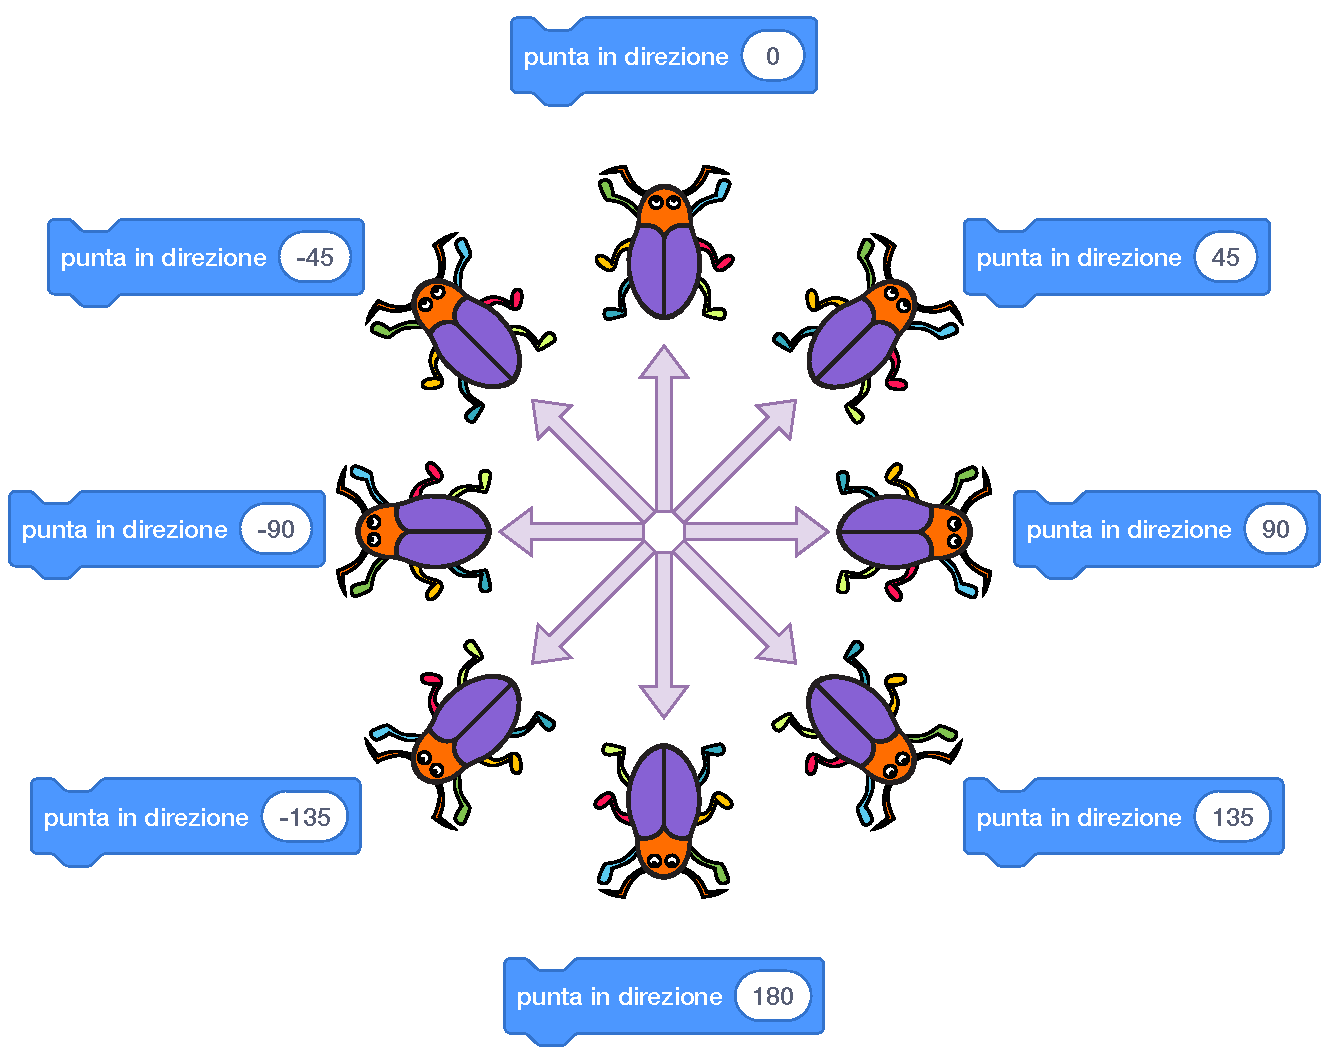
\includegraphics[width=\linewidth]{img/scratchblocks-cap08/pdf/figure-rosa-venti.pdf}\label{credito:figure-rosa-venti-1}
  \end{center}
  \caption{Effetti del blocco \textbf{punta in direzione...}}
  \label{fig:direzioni-assolute}
\end{figure}



Esiste anche un secondo modo per cambiare direzione: la \textbf{rotazione relativa}. È simile ai comandi ``gira a sinistra'' e ``gira a destra'' visti nel Capitolo~\ref{capitolo-7-code.org} su Code.org, ma in Scratch si realizza tramite i blocchi 
\includegraphics[width=107bp]{img/scratchblocks-cap08/pdf/scratch-ruota-orario.pdf}\label{credito:scratch-ruota-orario-1} (\textbf{Movimento}), in senso orario o antiorario, indicato dalla freccia sul blocco (vedi Figura~\ref{fig:direzioni-relative}).

Questi blocchi fanno ruotare lo sprite attorno al proprio centro e di un angolo dell'ampiezza in gradi indicata rispetto alla direzione in cui sta guardando in quel momento, e non verso una direzione assoluta. Richiedono familiarità con il concetto di angolo, che in terza primaria potrebbe non essere ancora stato affrontato formalmente, ma questi blocchi possono essere utili per comprendere meglio come funziona il movimento e per rispondere agli errori più comuni degli alunni.

\begin{figure}[!htb]
  \centering
  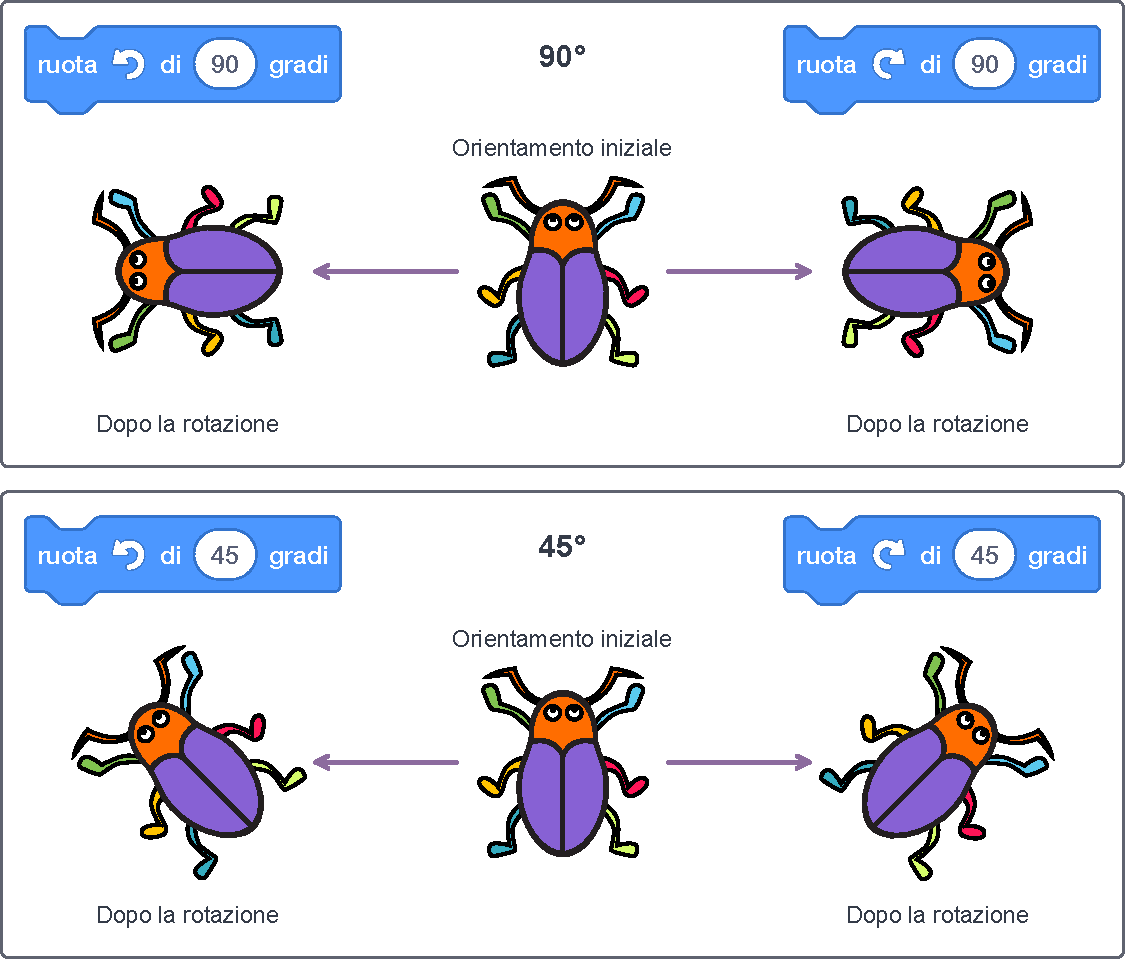
\includegraphics[width=\linewidth]{img/scratchblocks-cap08/pdf/figure-angoli.pdf}
  \label{credito:figure-angoli-1}
  \caption{Effetti del blocco \textbf{ruota...}}
  \label{fig:direzioni-relative}
\end{figure}

\subsection{Approfondimento: spostamenti}\label{approfondimento-spostamenti-assoluti-e-relativi}

I comandi di movimento disponibili in Scratch sono molti di più di quelli proposti nelle attività viste finora. È possibile che alcuni vengano scoperti da alunni e alunne spontaneamente esplorando l'interfaccia: per questo motivo offriamo qui una breve spiegazione aggiuntiva, così da poter rispondere con sicurezza alle loro domande.

Nelle attività precedenti abbiamo usato soprattutto il blocco 
\includegraphics[width=78bp]{img/scratchblocks-cap08/pdf/scratch-faipassi.pdf}\label{credito:scratch-faipassi-1}. Per confrontarlo con gli altri comandi, distinguiamo due modi di indicare uno spostamento:

\begin{itemize}
\item
  \textbf{Movimento relativo}: si indica di quanto modificare la posizione attuale. Con 
\includegraphics[width=78bp]{img/scratchblocks-cap08/pdf/scratch-faipassi.pdf}\label{credito:scratch-faipassi-2}, lo spostamento dipende anche dalla direzione in cui sta guardando lo sprite: per esempio, 
\includegraphics[width=78bp]{img/scratchblocks-cap08/pdf/scratch-fai10.pdf}\label{credito:scratch-fai10-3} fa avanzare lo sprite di 10 passi (cioè 10 unità dello stage), a partire dalla posizione in cui si trova, nella direzione in cui sta guardando. Se, anche partendo dalla stessa posizione, avesse avuto lo sguardo puntato in un'altra direzione, la posizione di arrivo sarebbe stata diversa;
\item
  \textbf{Movimento assoluto}: si indica la posizione da raggiungere tramite le coordinate dello stage. La direzione dello sguardo non influisce e non viene cambiata. Per esempio, il comando 
\includegraphics[width=103bp]{img/scratchblocks-cap08/pdf/testo-vai-100-0.pdf}\label{credito:testo-vai-100-0-1}, qualunque sia la posizione di partenza dello sprite e la direzione iniziale verso cui guarda, porta lo sprite nel punto (100, 0) dello stage lasciando invariata la direzione.
\end{itemize}

\begingroup
\manualeimpostazioni
\setlength{\LTleft}{0pt}
\setlength{\LTright}{0pt}
\newcommand{\bloccotabellamovimento}[2]{%
  \manualeimmagini{\includegraphics[width=#1]{#2}}}
\begin{longtable}{|K{\dimexpr0.47\linewidth-2\tabcolsep-1.5\arrayrulewidth\relax}|J{\dimexpr0.53\linewidth-2\tabcolsep-1.5\arrayrulewidth\relax}|}
\arrayrulecolor{guideManualeBordo}
\hline
\manualetitolo{2}{SPOSTAMENTI SCRATCH}
\manualeintestazione
\endfirsthead
\hline
\manualetitolo{2}{SPOSTAMENTI SCRATCH}
\manualeintestazione
\endhead
\bloccotabellamovimento{78bp}{img/scratchblocks-cap08/pdf/scratch-faipassi.pdf}\label{credito:scratch-faipassi-3} & Sposta lo sprite del numero di passi (unità, pixel) indicato, a partire dalla posizione attuale e nella sua direzione corrente. Con un valore negativo si muove nel verso opposto, senza cambiare direzione dello sguardo. \\
\hline
\bloccotabellamovimento{98.5bp}{img/scratchblocks-cap08/pdf/scratch-vai-a.pdf}\label{credito:scratch-vai-a-2} & Porta istantaneamente lo sprite nel punto di coordinate (\emph{x}, \emph{y}), senza cambiarne la direzione. \\
\hline
\bloccotabellamovimento{180bp}{img/scratchblocks-cap08/pdf/scratch-scivola.pdf}\label{credito:scratch-scivola-1} & Porta lo sprite nel punto di coordinate (\emph{x}, \emph{y}) nel tempo indicato, senza cambiarne la direzione. A parità di percorso, più tempo significa minore velocità. \\
\hline
\bloccotabellamovimento{82.5bp}{img/scratchblocks-cap08/pdf/tabella-posizione-xy.pdf}\label{credito:tabella-posizione-xy-1} & Imposta la coordinata \emph{x} oppure \emph{y} al valore indicato, e quindi sposta istantaneamente lo sprite lasciando invariate l'altra coordinata e la direzione. \\
\hline
\bloccotabellamovimento{81bp}{img/scratchblocks-cap08/pdf/tabella-variazione-xy.pdf}\label{credito:tabella-variazione-xy-1} & Aggiunge il valore indicato al valore della coordinata \emph{x} oppure \emph{y} attuale: lo spostamento avviene parallelamente all'asse corrispondente, senza cambiare la direzione dello sprite né dipendere da essa. \\
\hline
\bloccotabellamovimento{131.5bp}{img/scratchblocks-cap08/pdf/scratch-rimbalza.pdf}\label{credito:scratch-rimbalza-1} & Se lo sprite tocca un bordo, si allontana dal bordo
come se avesse colpito una superficie rigida. \\
\hline
\bloccotabellamovimento{159.5bp}{img/scratchblocks-cap08/pdf/scratch-stile-rotazione.pdf}\label{credito:scratch-stile-rotazione-1} & Permette di selezionare lo stile di rotazione: sinistra-destra significa che lo sprite può guardare a sinistra e a
destra, ma non si inclinerà. \\
\hline
\end{longtable}
\manualeripristinacolore
\endgroup




\newpage
\Needspace{10\baselineskip}
\begin{consiglio}[Maestr* si è buggato... non si muove!]

\noindent
\begin{minipage}[t]{0.28\linewidth}
\vspace{0pt}
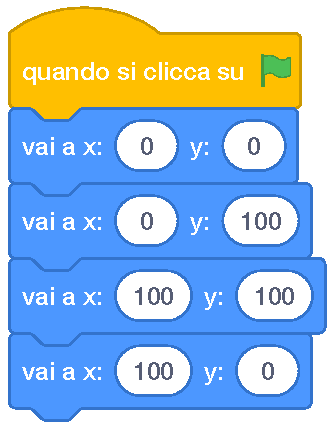
\includegraphics[width=107.5bp]{img/scratchblocks-cap08/pdf/scratch-vai-inutili.pdf}\label{credito:scratch-vai-inutili-1}
\end{minipage}\hfill
\begin{minipage}[t]{0.68\linewidth}
\vspace{0pt}
Può capitare che, anche usando i blocchi di movimento corretti, lo sprite sembri non spostarsi alle coordinate indicate, come nel programma a fianco (provatelo!). In realtà si sta muovendo eccome, ma così velocemente che l'occhio non fa in tempo a percepire il cambiamento. Per questo motivo, dal punto di vista grafico il programma qui a fianco è equivalente al solo ultimo blocco.
\end{minipage}

Per rendere visibile il movimento potete:

\begin{itemize}
  \item inserire un blocco 
\includegraphics[width=97bp]{img/scratchblocks-cap08/pdf/scratch-attendi.pdf}\label{credito:scratch-attendi-2} tra un movimento e l'altro, così lo sprite farà una piccola pausa prima del passo successivo;
  \item oppure usare il blocco 
\includegraphics[width=180bp]{img/scratchblocks-cap08/pdf/scratch-scivola.pdf}\label{credito:scratch-scivola-2}, che mostra il percorso sullo stage in modo fluido e chiaro.

\end{itemize}



\end{consiglio}

\begin{consiglio}[Maestr* come faccio ad andare indietro?]


\includegraphics[width=78bp]{img/scratchblocks-cap08/pdf/scratch-faipassi.pdf}\label{credito:scratch-faipassi-4}In Scratch il blocco \textbf{fai \ldots{} passi} fa muovere lo sprite nella direzione in cui sta guardando. Per andare nella direzione opposta non serve un blocco nuovo: basta usare un numero negativo. Per esempio, il valore -10 nel blocco 
\includegraphics[width=81bp]{img/scratchblocks-cap08/pdf/testo-passi-negativi.pdf}\label{credito:testo-passi-negativi-1} fa muovere lo sprite di 10 passi nel verso opposto a dove sta guardando. Questo è un ottimo momento per far notare a bambini e bambine che anche i numeri con il segno davanti hanno un effetto preciso sul movimento. Non è necessario formalizzare i numeri negativi dal punto di vista matematico: si tratta di sperimentare e osservare cosa succede allo sprite quando si cambia il valore numerico nel blocco.

\end{consiglio}


\section{Attività 6: sperimentare programmi}

\ruoliattivita{\ruoloProgrammatore}

In questa attività alunne e alunni copiano in Scratch alcuni programmi già pronti, per scoprire che effetto hanno.

Per esempio, puoi fornire loro questi programmi:

\begin{center}
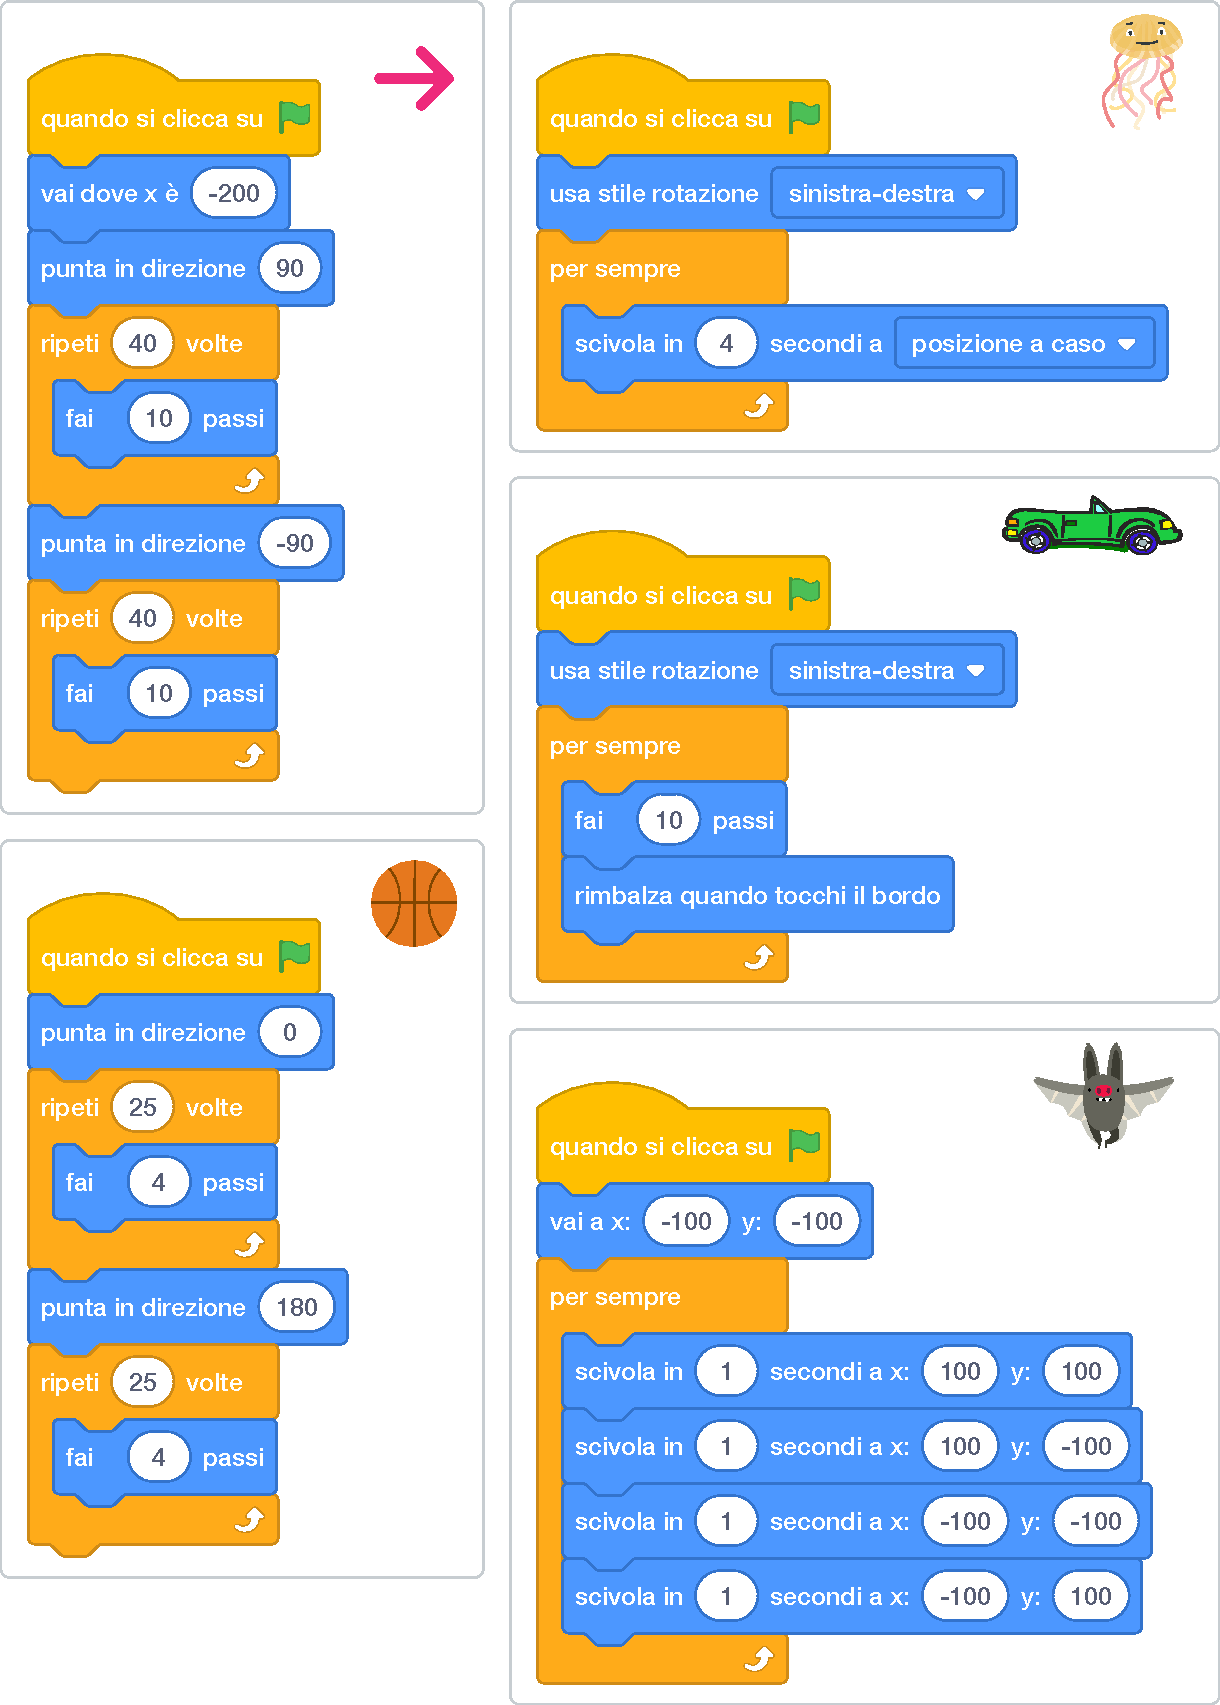
\includegraphics[width=\linewidth]{img/scratchblocks-cap08/pdf/figure-sperimentare-programmi.pdf}\label{credito:figure-sperimentare-programmi-1}
\end{center}


Copiare e provare i programmi già pronti è un modo efficace per imparare a programmare, soprattutto se accompagnati da domande che stimolano la riflessione. Mentre ricostruiscono i blocchi uno alla volta, gli alunni e le alunne osservano cosa succede sullo schermo, fanno ipotesi, notano differenze e scoprono nuovi concetti senza bisogno di spiegazioni astratte. Questo approccio offre la possibilità di:

\begin{itemize}
\item
  imparare osservando cosa fa ogni blocco;
\item
  capire la struttura del programma semplicemente ricreandolo;
\item
  esplorare idee nuove in modo guidato ma creativo;
\item
  aumentare il proprio senso di sicurezza riproducendo un codice che funziona.
\end{itemize}

È un po' come quando si impara a leggere copiando parole: prima si imita, poi si diventa capaci di crearne di nuove. Copiare programmi non è solo utile: è un passo fondamentale per costruire autonomia e padronanza nella programmazione.

Alcuni suggerimenti operativi:

\begin{itemize}
\item
  Dopo aver copiato un programma e prima di eseguirlo, invitate bambini e bambine a rispondere alla domanda: ``Secondo te cosa succederà?''
\item
  Chiedete agli alunni e alle alunne di modificarne un solo elemento: ad esempio un numero, un blocco, un costume o una direzione. Una variazione alla volta aiuta a capire quale blocco produce quale effetto.
\end{itemize}

\section{Attività 7: solo 10 blocchi!}

\ruoliattivita{\ruoloProgrammatore}

Questa sfida riprende l'attività ``10 Blocchi'' della guida \textit{Creative Computing} di \citeauthor{brennan-creative-computing}, disponibile anche nella traduzione italiana (pp.~30--31; \linkbreve{scratchGuida}).

In questa sfida gli alunni e le alunne devono inventare un programma usando soltanto i dieci tipi di blocco proposti di seguito. Ogni tipo deve comparire almeno una volta, ma può essere usato anche più volte. Alcuni blocchi li conoscono già, altri li scopriranno giocando e sperimentando! Aiutate gli alunni a cercare i blocchi nell'Area dei blocchi in base ai colori.

\begin{center}
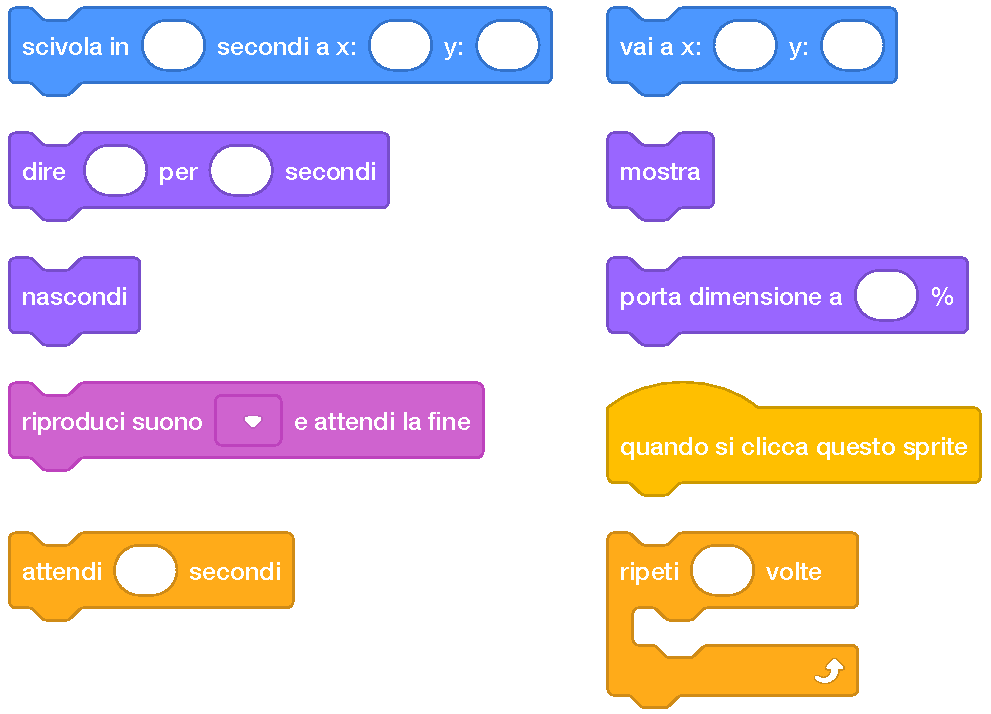
\includegraphics[width=0.92\linewidth]{img/scratchblocks-cap08/pdf/scratch-10blocchi.pdf}\label{credito:scratch-10blocchi-1}
\end{center}


A differenza della ``tela bianca'' di Scratch, che permette di usare subito tutti i comandi disponibili, qui si lavora entro un insieme ristretto di blocchi. Questo non è un limite: anzi, i vincoli diventano un motore per la creatività. Quando le possibilità sono definite, si è spinti a esplorare ogni blocco, anche quelli che normalmente verrebbero ignorati, e a combinarli in modi nuovi.

Per questo tipo di attività, l'insegnante può creare altre sfide scegliendo set diversi di blocchi (per esempio prendendone 7 o 8). L'importante è che i blocchi selezionati permettano comunque di costruire programmi vari e significativi, possibilmente diversi da quelli già realizzati in classe, così da ampliare l'immaginario di ciascuno e stimolare nuove idee.

\section{Bonus: costumi e suoni }\label{bonus-costumi-e-suoni}

\ruoliattivita{\ruoloProgrammatore}

\noindent
\begin{minipage}[c]{0.44\linewidth}
\centering
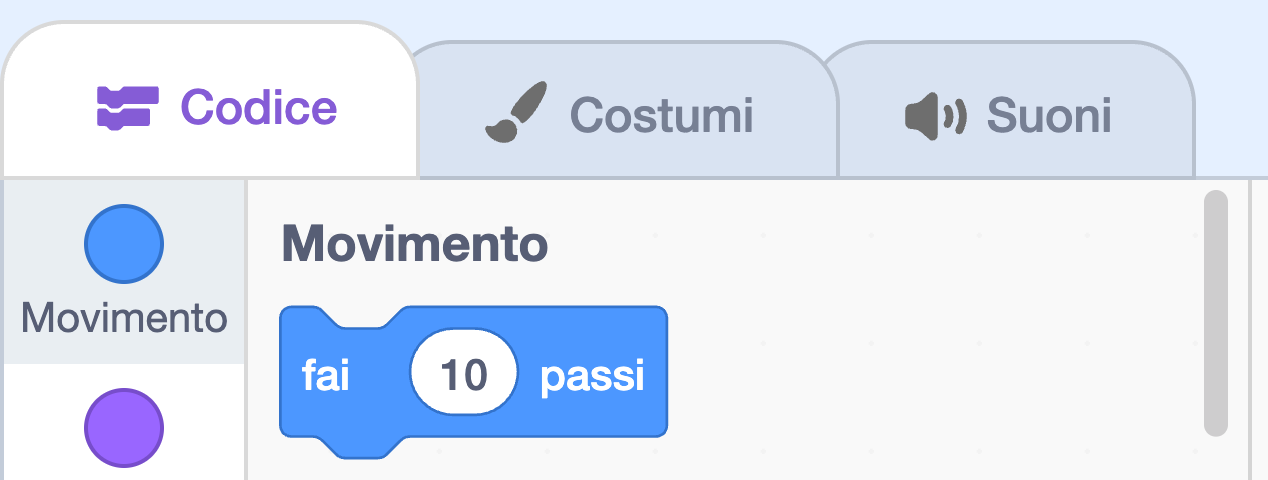
\includegraphics[width=\linewidth]{img/scratch-linguette.png}\label{credito:scratch-linguette-1}
\end{minipage}\hfill
\begin{minipage}[c]{0.52\linewidth}
Per concludere, parliamo di due funzionalità interessanti da presentare in classe: costumi e suoni. Alcuni degli sprite di Scratch hanno a disposizione diversi \textbf{costumi}, cioè immagini alternative con aspetti o posizioni differenti. Allo stesso modo, ogni sprite può essere associato a uno o più \textbf{suoni}, che possono essere riprodotti dalle casse del computer.
\end{minipage}
\par

È possibile vedere costumi e suoni associati allo sprite cliccando sulle linguette a fianco della linguetta codice, in alto sopra l'Area dei blocchi. Per tornare al codice, è sufficiente cliccare sulla linguetta corrispondente. Nella scheda ``Costumi'' è possibile scegliere costumi, disegnarne di nuovi, duplicarli o modificarli. I costumi permettono di trasformare lo sprite in modo creativo, ad esempio cambiando espressione, postura, colori o dettagli del personaggio.

Sono anche uno strumento importante per creare \textbf{animazioni}: alternando due o più costumi e combinandoli con blocchi di movimento, si può simulare l'effetto di un personaggio che cammina, corre o sbatte le ali. Nello sprite dell'ippopotamo, per esempio, esistono due costumi che mostrano le ali in posizioni diverse (su/giù): utilizzando il blocco 
\includegraphics[width=115.5bp]{img/scratchblocks-cap08/pdf/scratch-costume-seguente.pdf}\label{credito:scratch-costume-seguente-1} (\textbf{Aspetto}) dentro una ripetizione per sempre è possibile fare battere le ali al nostro ippopotamo.


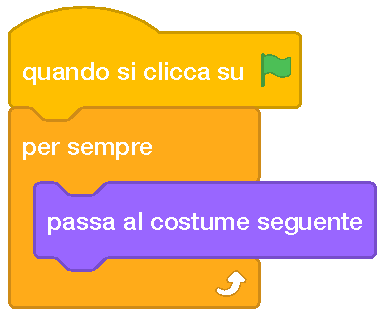
\includegraphics[width=123bp]{img/scratchblocks-cap08/pdf/scratch-ripeti-costume.pdf}\label{credito:scratch-ripeti-costume-1}


\noindent
\begin{minipage}[c]{0.81\linewidth}
Per creare un \textbf{nuovo suono} bisogna premere sull'icona con l'altoparlante e scegliere uno dei modi possibili (dall'alto verso il basso):

\begin{itemize}
\item
  caricare un file audio dal computer;
\item
  far scegliere a Scratch un suono dalla libreria in maniera casuale;
\item
  registrarlo;
\item
  sceglierlo dalla libreria di Scratch.
\end{itemize}
\end{minipage}\hfill
\begin{minipage}[c]{0.15\linewidth}
\centering

\includegraphics[height=1.4in]{img/scratch-scegli-suono.png}\label{credito:scratch-scegli-suono-1}
\end{minipage}
\par

È poi possibile riprodurre il suono scelto con il blocco 
\includegraphics[width=180bp]{img/scratchblocks-cap08/pdf/scratch-suono.pdf}\label{credito:scratch-suono-1} (\textbf{Suono}).



\section{Modalità di lavoro }\label{modalituxe0-di-lavoro-5}

\subsection{Programmazione in coppia }\label{programmazione-in-coppia-1}

Nel Capitolo~\ref{capitolo-7-code.org} abbiamo introdotto la metodologia della programmazione in coppia (\ref{programmazione-in-coppia}), evidenziando i ruoli di \textbf{pilota} e \textbf{navigatore}. Quel modello resta valido anche in Scratch: lavorare in coppia è un potente strumento per favorire attenzione, verbalizzazione, confronto, pianificazione e debugging.

In Scratch però il contesto cambia. Non ci sono puzzle da risolvere, né un pulsante dedicato a tracciare automaticamente il lavoro dei partner. Qui gli alunni e le alunne non si limitano a seguire un percorso guidato: progettano liberamente storie, dialoghi, animazioni e movimenti sullo stage. Questo rende la collaborazione ancora più preziosa, perché richiede decisioni condivise su cosa fare, come farlo e perché. Alcuni consigli per aiutare le coppie a collaborare:

\begin{itemize}
\item
  invitali a discutere e concordare insieme la scena da realizzare prima di iniziare a programmare;
\item
  chiedi al pilota di raccontare le proprie scelte;
\item
  ricorda a ciascuna coppia di scambiarsi i ruoli regolarmente.
\end{itemize}

\subsection{Usa-Modifica-Crea (UMC) }\label{usa-modifica-crea-umc}

Anche in Scratch ritroviamo l'approccio UMC (\ref{usa-modifica-crea}), già introdotto nel Capitolo~\ref{capitolo-7-code.org}: si parte da programmi esistenti, si esplorano piccole modifiche e poi si arriva alla creazione di progetti personali. La logica di fondo resta la stessa, ma in Scratch assume una forma più aperta e creativa.

\begin{itemize}
\item
  \textbf{Usa}: alunni e alunne provano programmi già costruiti dall'insegnante (per esempio animazioni o dialoghi) e osservano che cosa succede sullo stage, senza dover ricostruire tutto da zero.
\item
  \textbf{Modifica}: alunni e alunne cambiano numeri, blocchi, direzioni, costumi o tempi, prima facendo previsioni e poi confrontando previsione e risultato. Anche un singolo cambiamento può trasformare in modo evidente il comportamento dello sprite.
\item
  \textbf{Crea}: grazie alla libertà di movimento nello stage, ai costumi, ai suoni e ai dialoghi, la fase di creazione diventa naturalmente più ampia: ciascuno può progettare qualcosa di unico, non solo una variante del modello di partenza.
\end{itemize}

In Scratch, quindi, l'UMC mantiene la struttura per proporre i concetti, ma si arricchisce di un elemento nuovo: non si risolve un problema dato, si progetta un'idea personale. Questo valorizza il pensiero creativo e la progettazione autentica, mettendo al centro l'immaginazione di alunni e alunne.

\section{Aspetti informatici }\label{aspetti-informatici-4}

In questo capitolo, alunni e alunne continuano a lavorare con un linguaggio di programmazione visuale, ritrovando molti concetti già incontrati con Code.org: \textbf{sintassi} (i blocchi si incastrano solo in certi modi), \textbf{semantica} (ogni blocco ha un significato preciso), \textbf{esecutore meccanico} (lo sprite fa solo ciò che è scritto), \textbf{algoritmi} e \textbf{programmi}, \textbf{sequenza} e \textbf{ripetizioni}, \textbf{parametri} e \textbf{debugging}. La logica di fondo non cambia: un programma è una sequenza di istruzioni che il computer esegue alla lettera.

Quello che cambia è l'ambiente: in Scratch il programmatore deve ragionare non solo su \textbf{cosa} fare, ma anche su \textbf{dove} farlo accadere e su \textbf{come} un personaggio può comportarsi nel tempo. Questo introduce alcune idee nuove e importanti.

\begin{itemize}
\item
  \textbf{Creatività e progettazione libera.} A differenza dei puzzle proposti in Code.org, qui non c'è un obiettivo già definito da raggiungere. Alunni e alunne devono decidere che cosa vogliono ottenere: una scena, un dialogo, un'animazione, una storia, un gioco. L'informatica non è più solo trovare la soluzione corretta a un problema dato, ma immaginare il problema stesso e costruire un percorso per risolverlo. La dimensione creativa non è un'aggiunta estetica: è parte centrale della competenza informatica, perché costringe a fare scelte, a definire scopi e a trasformarli in istruzioni chiare.
\item
  \textbf{Debugging come ricerca del risultato desiderato}. In questo contesto il debugging assume un significato diverso rispetto ai puzzle: non si tratta più soltanto di far funzionare il programma nel modo ``giusto'', ma di capire perché il comportamento osservato è diverso da quello voluto. Bambini e bambine devono confrontare l'idea che avevano con ciò che accade sullo stage, e rivedere il codice fino a ottenere l'effetto desiderato. Questo rende il debugging un processo più aperto e riflessivo, dove si impara dai propri tentativi, invece di inseguire un'unica risposta esatta.
\end{itemize}

\section{Relazione con l'informatica nelle Indicazioni Nazionali 2025 }\label{relazione-con-linformatica-nelle-indicazioni-nazionali-5}

Relativamente alle Indicazioni Nazionali 2025, queste attività contribuiscono allo sviluppo delle seguenti competenze, obiettivi e conoscenze (queste ultime inserite nelle Indicazioni Nazionali 2025 a titolo di esempio, non prescrittive).


\subsubsection{Competenze (alla fine della scuola primaria) nella disciplina Matematica}


\begin{itemize}
\item
  \emph{Scrivere e comprendere semplici programmi, espressi in elementari linguaggi di programmazione a scopo didattico, e valutarne l'adeguatezza rispetto al compito che si vuole automatizzare.}
\end{itemize}


\subsubsection{Competenze (alla fine della scuola primaria) nella disciplina Tecnologia}


\begin{itemize}
\item
  \emph{Sviluppare un atteggiamento positivo nei confronti delle applicazioni informatiche riconoscendone le potenzialità come strumenti di espressione personale nella vita quotidiana.}
\end{itemize}



\subsubsection{Obiettivi (alla fine della terza primaria) nella disciplina Matematica}


\begin{itemize}
\item
  \emph{Scrivere semplici programmi e verificare, mediante la loro esecuzione, se svolgono il compito previsto ed eventualmente correggerli.}
\end{itemize}


\subsubsection{Obiettivi (alla fine della terza primaria) nella disciplina Tecnologia}


\begin{itemize}
\item
  \emph{Creare, selezionare e usare semplici testi o disegni, usando strumenti informatici.}
\end{itemize}



\subsubsection{Conoscenze (scuola primaria) nella disciplina Matematica}


\begin{itemize}
\item
  \emph{Concetto di algoritmo e sua esecuzione rigorosa.} In particolare qui si lavora sulla creazione ed esecuzione di programmi, cioè algoritmi scritti in un linguaggio di programmazione (qui, in particolare, il linguaggio Scratch);
\item
  \emph{Strutture di controllo fondamentali di un linguaggio di programmazione e reazione agli eventi.}
\item
  \emph{Controllo di correttezza dei programmi.}
\end{itemize}

\subsubsection{Conoscenze (scuola primaria) nella disciplina Tecnologia}

\begin{itemize}
\item
  \emph{Creazione e modifica di semplici contenuti digitali e multimediali usando semplici applicazioni informatiche, per raccontare storie o esperienze personali.}
\end{itemize}

\section{Valore costruzionista }\label{valore-costruzionista-5}

In Scratch l'apprendimento non nasce dalla ricerca della ``risposta giusta'', ma dalla costruzione di qualcosa di personale e significativo. Ogni progetto è un artefatto che prende forma nel tempo attraverso tentativi, modifiche e nuove idee. Questo modo di lavorare rispecchia l'idea dell'\textbf{apprendimento creativo}, al centro della spirale proposta da \textcite{resnick-2018}: immaginare → creare → giocare → condividere → riflettere, e di nuovo immaginare:

\begin{itemize}
\item
  \textbf{Immaginare}: ciascuno parte da un'idea propria, per esempio inventando una storia.
\item
  \textbf{Creare}: si traduce l'idea in blocchi di codice, costumi, movimenti e posizioni, scoprendo strumenti nuovi mentre vengono usati.
\item
  \textbf{Giocare}: si esegue il programma e si osserva cosa accade, divertendosi a modificare blocchi, numeri e costumi per vedere nuovi effetti.
\item
  \textbf{Condividere}: ciascuno mostra il proprio lavoro agli altri, facendoglielo provare e ascoltando idee e punti di vista diversi.
\item
  \textbf{Riflettere}: ci si accorge di cosa funziona e cosa no, e si cambia il progetto per migliorarlo o trasformarlo.
\end{itemize}

In classe questo processo appare molto chiaramente: il debugging non serve solo a correggere errori tecnici, ma a chiarire l'intenzione del progetto (``cosa volevo fare davvero?''), e ogni modifica apre possibilità nuove. L'attenzione si sposta dal risultato all'esperienza--una forma di apprendimento attivo che unisce creatività, logica e collaborazione.

\section{Suggerimenti per ulteriori attività}\label{suggerimenti-per-ulteriori-attivituxe0-e-riferimenti-5}

\printbibliography[heading=none,keyword={cap8},category={attivita}]

\begin{rimandiquaderno}
Se possiedi il volume studente \emph{Sulle orme di Milù -- Informatica}
(Mondadori Education, 2026), puoi usare i rimandi seguenti per affiancarlo
alle attività di questo capitolo.\par\smallskip

\begin{itemize}[leftmargin=*,itemsep=5pt,topsep=4pt]
\item \textbf{Benvenuti in Scratch! (Attività 1).} Le schede BENVENUTI IN SCRATCH (pagg.~36--37) accompagnano l'esplorazione dell'interfaccia e si possono tenere aperte mentre si riflette sulla funzione delle diverse aree della schermata.
\item \textbf{Diventa un regista con Scratch! (Attività 2).} Nelle schede DIVENTA UN REGISTA CON SCRATCH (pagg.~38--39) puoi seguire i passi indicati per scegliere un personaggio e fargli pronunciare due o tre frasi con i blocchi ``dire''.
\item \textbf{Dialogo tra due personaggi (Attività 3).} Nella scheda DIALOGO TRA DUE PERSONAGGI (pag.~40) è proposto il dialogo tra ippopotamo e ragnetto descritto nella guida.
\item \textbf{Movimenti precisi (Attività 4).} Nelle schede MOVIMENTI PRECISI, i box di pag.~42 guidano l'esplorazione delle proprietà dimensione e direzione; le attività di pag.~43 guidano l'esplorazione della posizione dello sprite.
\item \textbf{Posizionare un personaggio (Attività 5).} Nella scheda POSIZIONARE UN PERSONAGGIO (pag.~44) è proposto un programma analogo a quello della guida, da copiare passo per passo, per sperimentare diverse coordinate di partenza. In ALTRI BLOCCHI DI MOVIMENTO (pag.~45) si lavora sulle direzioni.
\item \textbf{Sperimentare programmi (Attività 6).} Nella scheda SPERIMENTARE PROGRAMMI (pag.~46) sono disponibili programmi già pronti da copiare in Scratch per scoprirne l'effetto.
\item \textbf{Solo 10 blocchi! (Attività 7).} Nella scheda SOLO 8 BLOCCHI! (pag.~47) è proposta una sfida analoga a quella dei 10 blocchi presentata nella guida.
\end{itemize}
\end{rimandiquaderno}

\section{Riferimenti}\label{riferimenti-cap8}

\printbibliography[heading=none,keyword={cap8},notcategory={attivita}]


% !TeX root = main.tex
\chapterimage{chapter-09-conclusioni.jpg}
\chapter{Conclusioni}\label{capitolo-9-conclusioni}
\flushbottom % Ripristina l’impaginazione ordinaria dopo il capitolo 7 e 8


Al termine di questo percorso, pensiamo che la nostra visione sia chiara: l'informatica non è una semplice abilità tecnica né un insieme di strumenti da saper usare. È una \textbf{disciplina scientifica}, con i suoi concetti fondanti, i suoi linguaggi e i suoi metodi, che studia come rappresentare ed elaborare informazioni in modo automatico. Al pari della matematica o delle scienze, offre una lente interpretativa sul mondo e fornisce strumenti concettuali per comprenderlo e agire in modo consapevole.

Questa prospettiva è oggi più rilevante che mai. Le alunne e gli alunni che incontriamo nelle classi del primo ciclo vivranno e lavoreranno in una società sempre più segnata dalla presenza dei sistemi digitali. Interagiranno quotidianamente con sistemi automatici che prendono decisioni, suggeriscono azioni, classificano informazioni e rispondono a istruzioni. Prepararli a comprendere questo futuro non significa insegnare loro a usare applicazioni specifiche, destinate a cambiare rapidamente, ma fornire basi solide per capire \textbf{come funzionano} questi sistemi e \textbf{come dialogare} con essi.

L'avvento e la diffusione dell'intelligenza artificiale rendono questa esigenza ancora più urgente. Se formiamo i nostri alunni e alunne ad essere bravi esecutori di istruzioni, li mettiamo in competizione diretta con macchine che, su quel terreno, sono destinate a superarli. Se invece li aiutiamo a diventare capaci di \textbf{pensare, formulare e valutare soluzioni e algoritmi}, allora l'intelligenza artificiale può diventare uno strumento potente al loro servizio.

Nella nostra visione, l'informatica, lungi dall'essere una disciplina solo tecnica, è strettamente legata allo sviluppo di competenze di \textbf{problem solving} consapevole e sistematico: non si tratta solo di trovare una risposta, ma di progettare una strategia, metterla alla prova, confrontarla con alternative e migliorarla progressivamente.

In questo processo, diventano centrali alcune competenze chiave. In primo luogo, la capacità di \textbf{esprimersi in modo chiaro e non ambiguo}: descrivere una procedura, scrivere un algoritmo o progettare un programma richiede precisione nel linguaggio e attenzione ai dettagli. In secondo luogo, la capacità di \textbf{immedesimarsi nell'altro}, che sia un compagno o una compagna di classe, un robot o un computer: bisogna saper anticipare come le istruzioni verranno interpretate, distinguendo ciò che è implicito per chi scrive da ciò che è esplicito per chi esegue. Infine, la capacità di \textbf{rivedere criticamente il proprio lavoro}, osservando gli effetti delle istruzioni date, individuando errori o ambiguità e correggendoli mediante pratiche di debugging. In questo quadro, l'errore diventa un comportamento da accogliere e osservare, assumendo un ruolo centrale e positivo.

Tutto questo non può essere rimandato ai gradi di istruzione superiori. Al contrario, richiede un lavoro paziente e progressivo che può e deve iniziare fin dai primi anni. Le attività unplugged, i giochi di movimento su griglia, la rappresentazione delle informazioni, la risoluzione di problemi e, più avanti, la programmazione visuale e creativa mostrano che è possibile introdurre concetti informatici profondi in modo accessibile, concreto e significativo già nella scuola primaria e poi proseguire nella scuola secondaria di primo grado.


\backmatter
% Generato da aggiorna-link.py a partire dal registro YAML dei redirect.
% Non modificare a mano: rigenerare e conservare questo file nel repository.
% Capitolo finale non numerato; compare nell'indice e nei segnalibri PDF.
\chapterimage{chapter-sitografia.png}
\chapter*{Sitografia}
\addcontentsline{toc}{chapter}{Sitografia}
\markboth{\sffamily\normalsize\bfseries Sitografia}{}
\label{sitografia}

Gli indirizzi brevi usati nel testo, nelle note, nei crediti e nelle bibliografie
sono raccolti qui in ordine alfabetico, accanto alle rispettive destinazioni
complete. Puoi digitare gli indirizzi brevi così come sono stampati, rispettando
le maiuscole presenti nei nomi, per esempio \texttt{codeA}.

\begingroup
\footnotesize
\urlstyle{guida}
% Mantiene unito ://, lasciando spezzabile il resto degli URL.
\appto\UrlNoBreaks{\do\:}
\setlength{\tabcolsep}{5pt}
\renewcommand{\arraystretch}{1.15}
\begin{longtable}{@{}>{\raggedright\arraybackslash}p{.46\textwidth}>{\raggedright\arraybackslash}p{\dimexpr.54\textwidth-10pt\relax}@{}}
\textbf{Indirizzo breve} & \textbf{Destinazione completa}\\
\hline
\endfirsthead
\textbf{Indirizzo breve} & \textbf{Destinazione completa}\\
\hline
\endhead
\hline
\multicolumn{2}{r}{\emph{Continua nella pagina seguente}}\\
\endfoot
\hline
\endlastfoot
\linkbreve{aladdinProposte} & \url{https://lonati.di.unimi.it/didainfo_2019-20/proposte_didattiche_aladdin.pdf} \\[4pt]
\linkbreve{artista} & \url{https://studio.code.org/projects/artist} \\[4pt]
\linkbreve{artistaBase} & \url{https://studio.code.org/projects/artist_k1/lang/it} \\[4pt]
\linkbreve{bebrasCostruzioni} & \url{https://bebras.it/platform/html/player_teacher.html?class=screenshot&code=2025_Q05_SWOAIDEI} \\[4pt]
\linkbreve{bebrasExplorer} & \url{https://bebras.it/explorer.html} \\[4pt]
\linkbreve{bebrasOrdine} & \url{https://bebras.it/platform/html/player_teacher.html?code=2019_Q15} \\[4pt]
\linkbreve{beebot} & \url{https://www.tts-group.co.uk/programmable-robots/bee-bot/} \\[4pt]
\linkbreve{bluebot} & \url{https://www.tts-international.com/tts-blue-bot-bluetooth-programmable-floor-robot/1015269.html} \\[4pt]
\linkbreve{codeA} & \url{https://studio.code.org/it/courses/coursea-2021/units/1/lessons/2/levels/1?no_redirect=1&lang=it-IT} \\[4pt]
\linkbreve{codeAguida} & \url{https://studio.code.org/it/courses/coursea-2021/units/1?no_redirect=1&lang=it-IT} \\[4pt]
\linkbreve{codeB} & \url{https://studio.code.org/it/courses/courseb-2021/units/1/lessons/3/levels/1?no_redirect=1&lang=it-IT} \\[4pt]
\linkbreve{codeBguida} & \url{https://studio.code.org/it/courses/courseb-2021/units/1?no_redirect=1&lang=it-IT} \\[4pt]
\linkbreve{codeC} & \url{https://studio.code.org/it/courses/coursec-2021/units/1/lessons/3/levels/1?no_redirect=1&lang=it-IT} \\[4pt]
\linkbreve{codeEs} & \url{https://studio.code.org/it/courses/coursea-2021/units/1/lessons/4/levels/6?no_redirect=1&lang=it-IT} \\[4pt]
\linkbreve{codeLabirinto} & \url{https://studio.code.org/it/courses/pre-express-2021/units/1/lessons/3/levels/6?no_redirect=1&lang=it-IT} \\[4pt]
\linkbreve{codeorgIscrizione} & \url{https://studio.code.org/it/users/sign_in?lang=it-IT} \\[4pt]
\linkbreve{codeRapido} & \url{https://studio.code.org/it/courses/express-2021/units/1/lessons/1/levels/9?no_redirect=1&lang=it-IT} \\[4pt]
\linkbreve{codeVideo} & \url{https://studio.code.org/it/courses/coursea-2021/units/1/lessons/4/levels/1?no_redirect=1&lang=it-IT} \\[4pt]
\linkbreve{coding} & \url{https://cris.unibo.it/retrieve/87553fc7-576b-46ab-a779-5c3d1e55d4a3/Itadinfo\%20coding.pdf} \\[4pt]
\linkbreve{codingBivio} & \url{https://web.media.mit.edu/~mres/papers/CACM-Coding-At-Crossroads.pdf} \\[4pt]
\linkbreve{codingBivioIT} & \url{https://stefanorini.medium.com/il-coding-a-un-bivio-8f3ce9b6c6fe} \\[4pt]
\linkbreve{codingPrimaria} & \url{https://issuu.com/elipublishing/docs/coding_pensiero_computazionale_web} \\[4pt]
\linkbreve{coppia} & \url{https://www.youtube.com/watch?v=sTJ85VIYDRE} \\[4pt]
\linkbreve{costruzionismo} & \url{https://inria.hal.science/hal-02378761v1/} \\[4pt]
\linkbreve{cubetto} & \url{https://primotoys.com/} \\[4pt]
\linkbreve{fiabe} & \url{https://www.quid-plus.com/wp-content/uploads/2022/01/attivita-unplugged.pdf} \\[4pt]
\linkbreve{guidaAccountDocente} & \url{https://www.scratchfoundation.org/learn/learning-library/teacher-accounts} \\[4pt]
\linkbreve{guidaPensiero} & \url{https://fablab.unitn.it/wp-content/uploads/2025/08/Handbook-A5.pdf} \\[4pt]
\linkbreve{indicazioni2025} & \url{https://www.mim.gov.it/documents/20182/10554370/curricolo_web.pdf} \\[4pt]
\linkbreve{informatica2025} & \url{https://mondodigitale.aicanet.it/wp-content/uploads/2026/07/Lodi_Lonati_MondoDigitale_ITA.pdf} \\[4pt]
\linkbreve{informaticaPrimaria} & \url{https://inria.hal.science/hal-02379212v1/document} \\[4pt]
\linkbreve{ingranaggi} & \url{https://lcl.media.mit.edu/resources/activity/week1/gears.it.pdf?pdf=gears.it} \\[4pt]
\linkbreve{itadinfo2025} & \url{https://www.ledizioni.it/stag/wp-content/uploads/2025/10/ITADINFO_def_web.pdf} \\[4pt]
\linkbreve{kidbots} & \url{https://www.csunplugged.org/en/topics/kidbots} \\[4pt]
\linkbreve{lcl} & \url{https://lcl.media.mit.edu/} \\[4pt]
\linkbreve{manzi} & \url{https://www.youtube.com/watch?v=gKQ7GbworSw&t=524s} \\[4pt]
\linkbreve{milu} & \url{https://www.mondadorieducation.it/catalogo/sulle-orme-di-milu-0074279/} \\[4pt]
\linkbreve{oraInformaticA} & \url{https://programmailfuturo.it/come/ora-dell-informatica} \\[4pt]
\linkbreve{ordinamento} & \url{https://www.nature.com/articles/s41562-025-02302-6} \\[4pt]
\linkbreve{panino} & \url{https://www.youtube.com/watch?v=cDA3_5982h8} \\[4pt]
\linkbreve{pifAlgoritmi} & \url{https://programmailfuturo.it/media/docs/Lezione-06-Algoritmi.pdf} \\[4pt]
\linkbreve{pifCorsi} & \url{https://programmailfuturo.it/come/primaria-2021/introduzione} \\[4pt]
\linkbreve{pifCorsoA} & \url{https://programmailfuturo.it/come/primaria-2021/corso-a} \\[4pt]
\linkbreve{pifCorsoB} & \url{https://programmailfuturo.it/come/primaria-2021/corso-b} \\[4pt]
\linkbreve{pifIscrizione} & \url{https://programmailfuturo.it/chi/iscrizione-per-insegnanti/} \\[4pt]
\linkbreve{pifPensiero} & \url{https://programmailfuturo.it/media/docs/Lezione-03-Pensiero-Computazionale.pdf} \\[4pt]
\linkbreve{pifQuadretti} & \url{https://programmailfuturo.it/media/docs/Lezione-04-Programmazione-su-carta-a-quadretti-v2016.pdf} \\[4pt]
\linkbreve{programmazioneCode} & \url{https://edizionithemis.it/catalogo/libri-open-access/download/3-libri-open-access/1-la-programmazione-informatica-per-la-scuola-primaria} \\[4pt]
\linkbreve{scratch-beetle} & \url{https://assets.scratch.mit.edu/internalapi/asset/46d0dfd4ae7e9bfe3a6a2e35a4905eae.svg/get/} \\[4pt]
\linkbreve{scratchDocenti} & \url{https://scratch.mit.edu/educators} \\[4pt]
\linkbreve{scratchGuida} & \url{https://disi.unitn.it/~montreso/teacherdojo/2019/curriculum.pdf\#page=3} \\[4pt]
\linkbreve{talebot} & \url{https://www.matatastudio.com/tale-bot-pro.html} \\[4pt]
\linkbreve{tangram} & \url{https://thumb.wikimedia.org/wikipedia/commons/thumb/0/03/Tangrams_A4_Nevit.svg/1920px-Tangrams_A4_Nevit.svg.png} \\[4pt]
\linkbreve{umcCastello} & \url{https://dl.acm.org/doi/10.1145/3587102.3588793} \\[4pt]
\linkbreve{umcPercorsi} & \url{https://impactconectar.wixsite.com/website} \\[4pt]
\linkbreve{umcRicerca} & \url{https://www.tandfonline.com/doi/full/10.1080/08993408.2025.2542669} \\[4pt]
\linkbreve{unpluggedOrdini} & \url{https://classic.csunplugged.org/documents/books/italian/csunplugged-it.2015.1.0.pdf\#page=161} \\[4pt]
\linkbreve{unpluggedPesi} & \url{https://classic.csunplugged.org/documents/books/italian/csunplugged-it.2015.1.0.pdf\#page=101} \\[4pt]
\\
\end{longtable}
\endgroup

% Capitolo non numerato, successivo alla Sitografia.
\chapterimage{}
\chapterspaceabove{2.4cm}
\chapterspacebelow{0.4cm}
\chapter*{Attribuzioni e licenze dei materiali}
\addcontentsline{toc}{chapter}{Attribuzioni e licenze dei materiali}
\markboth{\sffamily\normalsize\bfseries Attribuzioni e licenze}{}
\label{attribuzioni-materiali}

I materiali di terzi conservano le licenze e le condizioni indicate qui, distinte dalla licenza generale della guida.

% Elimina i duplicati quando più immagini della stessa voce sono nella stessa pagina.
\ExplSyntaxOn
\seq_new:N \l_guida_crediti_pagine_seq
\seq_new:N \l_guida_crediti_etichette_seq
\tl_new:N \l_guida_crediti_pagina_tl
\NewDocumentCommand{\creditopagine}{m}
 {
  \group_begin:
  \seq_clear:N \l_guida_crediti_pagine_seq
  \seq_clear:N \l_guida_crediti_etichette_seq
  \clist_map_inline:nn {#1}
   {
    \tl_set:Nx \l_guida_crediti_pagina_tl {\getpagerefnumber{##1}}
    \seq_if_in:NVF \l_guida_crediti_pagine_seq \l_guida_crediti_pagina_tl
     {
      \seq_put_right:NV \l_guida_crediti_pagine_seq \l_guida_crediti_pagina_tl
      \seq_put_right:Nn \l_guida_crediti_etichette_seq {##1}
     }
   }
  \int_compare:nNnTF {\seq_count:N \l_guida_crediti_etichette_seq} > {1}
   {pp.\nobreakspace}{p.\nobreakspace}
  \seq_map_indexed_inline:Nn \l_guida_crediti_etichette_seq
   {
    \int_compare:nNnT {##1}>{1}{,~}
    \hyperlink{page.\getpagerefnumber{##2}}{\pageref*{##2}}
   }
  \group_end:
 }
\ExplSyntaxOff

\begingroup
\small

\section*{Schermate Code.org}
\textbf{Code.org (oggi CodeAI)}. I materiali curricolari e i tutorial sono distribuiti con licenza \hreforiginale{https://creativecommons.org/licenses/by-nc-sa/4.0/deed.it}{CC BY-NC-SA 4.0}.

Personaggi, icone, adesivi e motivi conservano i diritti dei rispettivi titolari. Per gli elementi esclusi dalla licenza Creative Commons, si richiama l’uso illustrativo didattico e non commerciale ai sensi dell’art. 70 della legge 22 aprile 1941, n. 633.

Le schermate provengono dalle seguenti fonti:
\begin{itemize}[leftmargin=*,itemsep=3pt,topsep=3pt,parsep=0pt]
\item \hrefbreve{codeEs}{Corso A (2021), lezione 4, livello 6} (\creditopagine{credito:codeorg-interfaccia-gioco-1,credito:codeorg-interfaccia-istruzioni-1,credito:codeorg-interfaccia-blocchi-1,credito:codeorg-interfaccia-lavoro-1,credito:codeorg-interfaccia-pulsanti-1,credito:codeorg-interfaccia-pulsanti-2,credito:codeorg-interfaccia-livelli-1}).
\item \hrefbreve{artistaBase}{Laboratorio Artista pre-scolare, in italiano} (\creditopagine{credito:codeorg-artista-menu-schema-1,credito:codeorg-artista-velocita-1,credito:codeorg-artista-scaletta-disegno-1,credito:codeorg-artista-quadrato-diagonale-disegno-1,credito:codeorg-artista-casa-strisce-disegno-1,credito:codeorg-artista-casa-disegno-1,credito:codeorg-artista-trama-disegno-1}).
\item \hreforiginale{https://studio.code.org/it/courses/coursec-2021/units/1/lessons/6/levels/2?lang=it&no_redirect=1}{Corso C (2021), lezione 6, livello 2} (\creditopagine{credito:codeorg-artista-selettore-angoli-1}).
\end{itemize}

\section*{Blocchi e programmi Code.org}
\textbf{Code.org (oggi CodeAI)} per blocchi, traduzioni e risorse dell’ambiente; trascrizioni e composizioni preparate per la guida. I blocchi sono ricostruiti in italiano senza lo sfondo dell’interfaccia. Valgono la CC BY-NC-SA 4.0 dei materiali didattici e le esclusioni relative alla grafica indicate sopra.

Il codice del motore è distribuito sotto \hreforiginale{https://github.com/code-dot-org/code-dot-org/blob/staging/LICENSE}{Apache 2.0}; questa licenza non si estende automaticamente all’intera figura. Il font incorporato \emph{Geist}, Copyright 2024 The Geist Project Authors, è distribuito sotto \hreforiginale{https://github.com/vercel/geist-font/blob/main/OFL.txt}{SIL Open Font License 1.1}.

\section*{Schermate e materiali Scratch}
\textbf{Scratch Foundation e partner.} Scratch is developed by the Scratch Foundation and its partners and affiliates. See \urloriginale{https://scratchfoundation.org/}. Secondo la \hreforiginale{https://mitscratch.freshdesk.com/en/support/solutions/articles/4000156890-can-i-use-screenshots-of-scratch-in-a-book-or-presentation-}{FAQ ufficiale}, le schermate di Scratch sono rilasciate con licenza Creative Commons Attribution-ShareAlike (\textbf{CC BY-SA}).

Le risorse della libreria storica di Scratch / Lifelong Kindergarten Group, MIT Media Lab, fra cui Ball-a e lo sfondo \hreforiginale{https://assets.scratch.mit.edu/internalapi/asset/9838d02002d05f88dc54d96494fbc202.png/get/}{Xy-grid}, sono distribuite sotto \hreforiginale{https://creativecommons.org/licenses/by-sa/2.0/deed.it}{CC BY-SA 2.0}.

\section*{Blocchi e composizioni Scratch}
Le figure sono ricostruite con \hreforiginale{https://github.com/scratchblocks/scratchblocks}{scratchblocks 3.7.1}, Copyright 2013--2021 Tim Radvan e collaboratori, \hreforiginale{https://github.com/scratchblocks/scratchblocks/blob/master/LICENSE}{licenza MIT}. Le icone derivano da Scratch Blocks, sotto \hreforiginale{https://www.apache.org/licenses/LICENSE-2.0}{Apache 2.0}.

\begin{itemize}[leftmargin=*,itemsep=3pt,topsep=3pt,parsep=0pt]
\item \hrefbreve{scratch-beetle}{\textbf{Beetle}} (\creditopagine{credito:figure-rosa-venti-1,credito:figure-angoli-1}): Scratch / Lifelong Kindergarten Group, MIT Media Lab; ridimensionato e ruotato per le due composizioni. Sprite e adattamenti: \textbf{CC BY-SA 2.0}.
\item \textbf{Arrow1-a, Basketball, Jellyfish-a, Convertible3 e Bat-a} (\creditopagine{credito:figure-sperimentare-programmi-1}): \hreforiginale{https://github.com/scratchfoundation/scratch-gui/blob/fa7ed724dd3070486ccf12424bd633f95572bdfd/src/lib/libraries/sprites.json}{libreria Scratch / Lifelong Kindergarten Group, MIT Media Lab}. Basketball e Bat: Alex Eben Meyer; Jellyfish: Daria Skrybchenko. Sprite ridimensionati; composizione per la guida in \textbf{CC BY-SA 2.0}.
\end{itemize}

\section*{Impaginazione e caratteri}
\begin{itemize}[leftmargin=*,itemsep=3pt,topsep=3pt,parsep=0pt]
\item \textbf{\hreforiginale{https://www.latextemplates.com/template/the-legrand-orange-book}{Legrand Orange Book 3.1}}, di Mathias Legrand e Vel / LaTeX Templates: modello adattato per questa edizione, CC BY-NC-SA 4.0.
\item \textbf{TeX Gyre Heros e Latin Modern Mono}, di Bogusław Jackowski e Janusz M. Nowacki: \hreforiginale{https://ctan.org/license/gfl}{GUST Font License}.
\item \textbf{Computer Modern}, di Donald E. Knuth, versioni Type 1 dell’American Mathematical Society: \hreforiginale{https://ctan.org/pkg/amsfonts}{SIL Open Font License 1.1}.
\item \textbf{Source Sans Pro}, di Paul D. Hunt, Adobe: \hreforiginale{https://github.com/adobe-fonts/source-sans/blob/release/LICENSE.md}{SIL Open Font License 1.1}.
\item \textbf{\hreforiginale{https://github.com/googlefonts/noto-emoji/blob/main/LICENSE}{Noto Color Emoji} e \hreforiginale{https://github.com/notofonts/noto-cjk/blob/main/Sans/LICENSE}{Noto Sans CJK SC}}, per emoji e caratteri cinesi: SIL Open Font License 1.1.
\item \textbf{Caratteri già incorporati nelle figure}: Helvetica Neue (Linotype/Adobe), Arial (Monotype). Conservano le rispettive licenze proprietarie.
\end{itemize}

\endgroup

% L'illustrazione A4 è centrata e rifilata ai bordi del foglio, senza deformarla.
\clearpage
\thispagestyle{empty}
\label{credito:chiusura}
\null
\begin{tikzpicture}[remember picture,overlay]
  \clip (current page.south west) rectangle (current page.north east);
  \node[inner sep=0pt] at (current page.center)
    {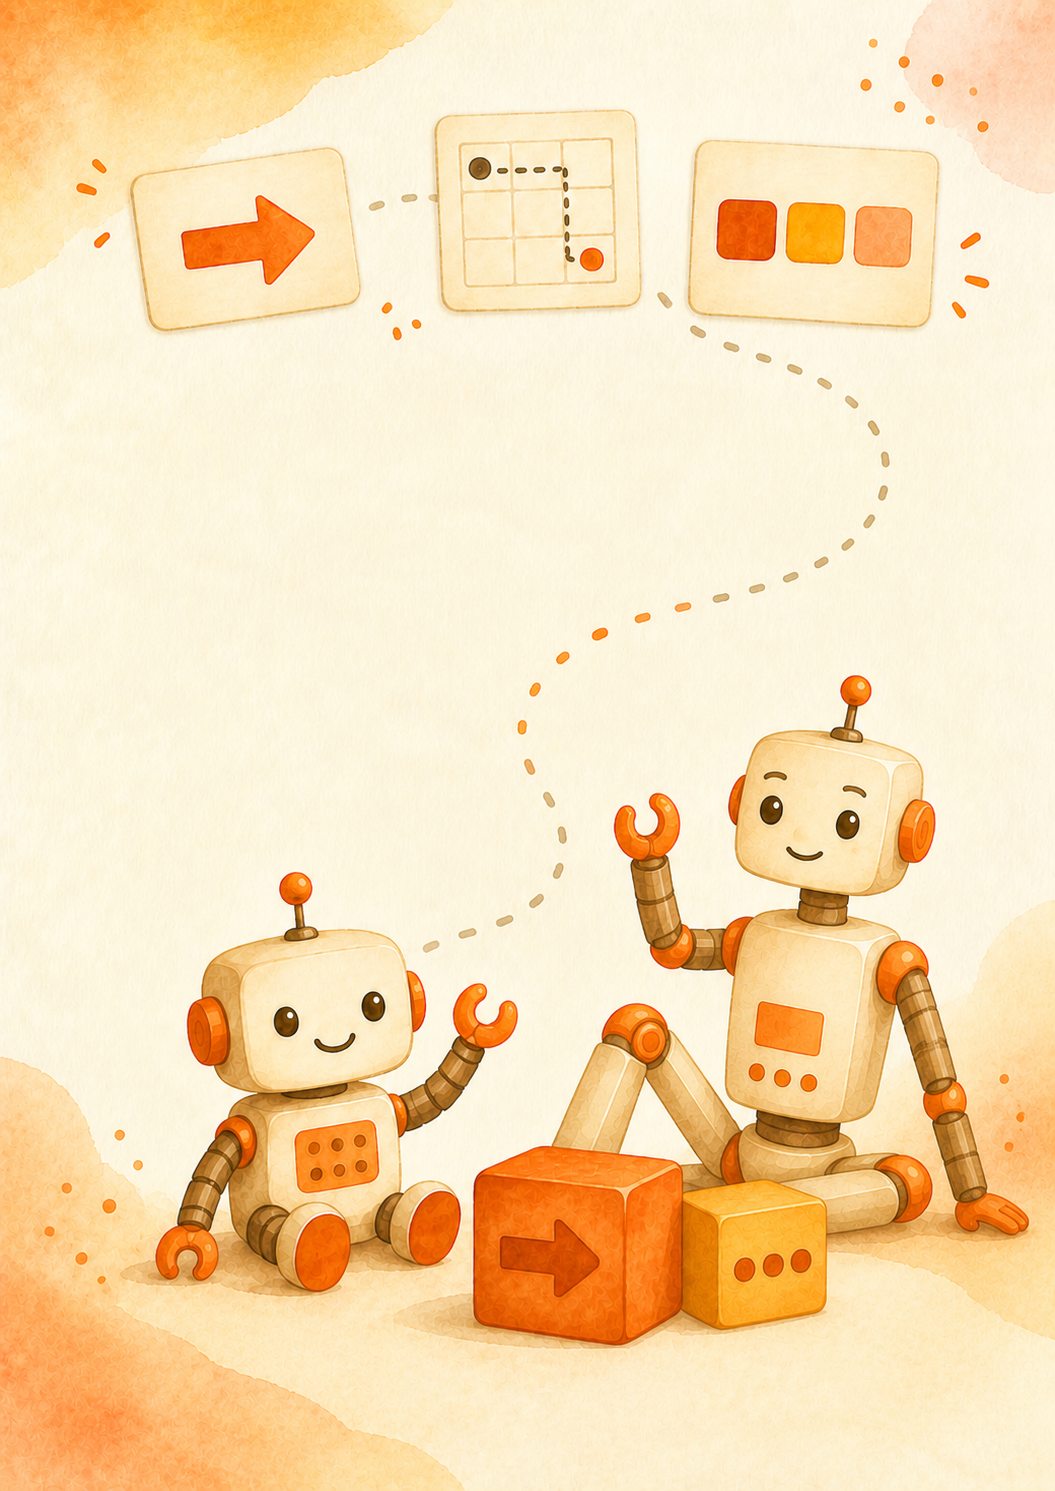
\includegraphics[height=\paperheight]{img/chiusura-illustrazione-arancione.png}};
\end{tikzpicture}
\clearpage
\end{document}
